% !TeX spellcheck = es_ES
\documentclass[11pt,a4paper,twoside]{report}

% ===== Paquetes esenciales =====
\usepackage[spanish]{babel}
\usepackage[utf8]{inputenc}
\usepackage[T1]{fontenc}
\usepackage{lmodern}
\usepackage{setspace}
\usepackage{hyperref}
\usepackage{fancyhdr}
\usepackage{graphicx}
\usepackage{geometry}
\usepackage{tocloft}
\usepackage{titlesec}
\usepackage{listings}
\usepackage{xcolor}
\usepackage{float}
\usepackage{url}
\usepackage{tikz}
\usepackage{courier}
\usepackage{pgfgantt}
\usepackage{enumitem}
\usepackage{placeins}
\usepackage{tocloft}
\usetikzlibrary{shapes, arrows, positioning}

\raggedbottom

\titlespacing*{\subsection}{0pt}{1em}{0.5em}

% ===== Configuraciones generales =====
\setlength{\headheight}{16pt}
\geometry{left=25mm, right=25mm, top=25mm, bottom=25mm}
\linespread{1.15} % Interlineado normativo

% ===== Encabezado y pie de página =====
\pagestyle{fancy}
\fancyhf{}
\fancyhead[LE,RO]{\textit{Utilización de un NIDS para redes SOHO (R-Snort)}}
\fancyfoot[CE,CO]{\thepage}

% ===== Formato de títulos =====
\titleformat{\chapter}[hang]{\bfseries\huge}{\thechapter.}{1pc}{}
\titlespacing*{\chapter}{0pt}{-10pt}{20pt}
\titleformat{\section}[hang]{\bfseries\Large}{\thesection.}{1pc}{}
\titleformat{\subsection}[hang]{\bfseries\large}{\thesubsection.}{1pc}{}
\renewcommand{\cftchapleader}{\cftdotfill{\cftdotsep}}

% Definición de colores si aún no los has puesto
\definecolor{mygreen}{rgb}{0,0.6,0}
\definecolor{mygray}{rgb}{0.5,0.5,0.5}
\definecolor{mymauve}{rgb}{0.58,0,0.82}

% Estilo snortstyle completo y compatible
% Estilo snortstyle completo y compatible
\lstdefinestyle{snortstyle}{
	backgroundcolor=\color{white},
	basicstyle=\footnotesize\ttfamily,
	breakatwhitespace=false,
	breaklines=true,
	captionpos=b,
	commentstyle=\color{mygreen},
	escapeinside={\%*}{*)},
	extendedchars=true,
	frame=single,
	keepspaces=true,
	keywordstyle=\color{blue},
	language=bash,
	morekeywords={sudo,systemctl,make,cmake,apt,tar,configure},
	numbers=left,
	numbersep=5pt,
	numberstyle=\tiny\color{mygray},
	rulecolor=\color{black},
	showspaces=false,
	showstringspaces=false,
	showtabs=false,
	stepnumber=2,
	stringstyle=\color{mymauve},
	tabsize=2,
	postbreak=\mbox{\textcolor{red}{$\hookrightarrow$}\space},
	title=\lstname,
	literate=
	{á}{{\'a}}1 {é}{{\'e}}1 {í}{{\'i}}1 {ó}{{\'o}}1 {ú}{{\'u}}1
	{Á}{{\'A}}1 {É}{{\'E}}1 {Í}{{\'I}}1 {Ó}{{\'O}}1 {Ú}{{\'U}}1
	{ñ}{{\~n}}1 {Ñ}{{\~N}}1 {¿}{{?`}}1 {¡}{{!`}}1
	{°}{{\textdegree}}1 {→}{{$\rightarrow$}}1 {⇒}{{$\Rightarrow$}}1
	{≥}{{$\geq$}}1 {≤}{{$\leq$}}1 {–}{{--}}1
	{“}{{``}}1 {”}{{''}}1 {’}{{'}}1 {•}{{\textbullet}}1
	{\{}{{\{}}1 {\}}{{\}}}1
	{\_}{{\_}}1 {\%}{{\%}}1 {\$}{{\$}}1
	{\\}{{\textbackslash}}1 {\#}{{\#}}1 {\&}{{\&}}1
	{\^}{{\^{}}}1 {\~}{{\~{}}}1 {\|}{{\textbar}}1
	{\033}{{\textbackslash033}}1,
}

% Activar el estilo globalmente
\lstset{style=snortstyle}

\lstdefinestyle{commandstyle}{
	backgroundcolor=\color{gray!10},
	basicstyle=\ttfamily\small,
	frame=single,
	breaklines=true,
	showstringspaces=false,
	columns=flexible,
	xleftmargin=1.5em,
	framexleftmargin=1.5em,
	keywordstyle=\color{blue},
	commentstyle=\color{mygreen},
	stringstyle=\color{mymauve},
	morekeywords={sudo,ls,cat,tail,echo,dig,nslookup,grep,awk,cut,printf,find},
	language=bash,
}

% ===== Inicio del documento =====
\begin{document}
	
	% ===== Portada (debes sustituirla por la oficial del Anexo II en la entrega) =====
	\begin{titlepage}
		\centering
		{\scshape\LARGE Universidad de Almería \par}
		\vspace{1cm}
		{\scshape\Large Complemento Trabajo Fin de Grado\par}
		\vspace{1.5cm}
		{\huge\bfseries Utilización de un NIDS para redes SOHO (R-Snort)\par}
		\vspace{2cm}
		{\Large Autor: Petrovics, Deian Orlando\par}
		\vspace{0.5cm}
		{\Large Tutor: Gómez López, Julio\par}
		\vspace{0.5cm}
		{\Large Cotutor: Padilla Soriano, Nicolás\par}
		\vfill
		{\large \today\par}
	\end{titlepage}
	
	\thispagestyle{empty}
	\cleardoublepage
	\thispagestyle{empty}
	
	
	
	% ===== Licencia Creative Commons =====
	\newpage
	\thispagestyle{empty}
	\begin{center}
		\vspace*{\fill}
		
\includegraphics[width=0.3\textwidth]{adicional/cc.xlarge.png}\\
		Este trabajo está bajo una licencia Creative Commons Atribución-NoComercial-CompartirIgual 4.0 Internacional.
		\vspace*{\fill}
	\end{center}
	
	\newpage
	\thispagestyle{empty}
	\null
	\newpage

	
	% ===== Índice =====

	\tableofcontents
	\newpage
	
	\listoffigures
	\newpage
	
	\listoftables
	\newpage
	
	\newcommand{\listoflistingscaption}{Índice de Códigos}
	
	\lstlistoflistings
	\newpage
	
	
	
	


% Abreviaturas
\chapter*{Abreviaturas}
\addcontentsline{toc}{chapter}{Abreviaturas}
\begin{itemize}
	\item \textbf{APT}: (Advanced Persistent Threat). Amenaza Avanzada Persistente. Suele involucrar ataques dirigidos y prolongados contra objetivos concretos.
	\item \textbf{ClamAV}: Antivirus de código abierto que analiza y detecta archivos maliciosos o infecciones. Se integra como complemento en el proyecto.
	\item \textbf{CPU}: (Central Processing Unit). Unidad central de procesamiento, comúnmente conocida como procesador, encargada de ejecutar instrucciones en un sistema.
	\item \textbf{CSV}: (Comma-Separated Values). Formato de archivo de texto plano que representa datos tabulares separados por comas o puntos y coma.
	\item \textbf{Debian Package (*.deb)}: Formato estándar de paquetes en sistemas GNU/Linux basados en Debian/Ubuntu. Facilita la instalación y gestión de software.
	\item \textbf{DoS}: (Denial of Service). Ataque que busca interrumpir el funcionamiento normal de un sistema o red.
	\item \textbf{FTP}: (File Transfer Protocol). Protocolo para la transferencia de archivos en redes IP.
	\item \textbf{GNU/Linux}: Sistema operativo de software libre en el que se basan distribuciones como Ubuntu, Debian, CentOS, etc.
	\item \textbf{HIDS}: (Host Intrusion Detection System). Sistema de Detección de Intrusiones basado en Host, centrado en vigilar el comportamiento interno de un equipo específico.
	\item \textbf{HTTP}: (Hypertext Transfer Protocol). Protocolo de comunicación utilizado en la web para transmitir información entre cliente y servidor.
	\item \textbf{HTTP2}: Segunda versión del protocolo HTTP, optimizada para mayor velocidad y eficiencia.
	\item \textbf{ICMP}: (Internet Control Message Protocol). Protocolo usado para enviar mensajes de error y diagnóstico en redes IP.
	\item \textbf{IDS}: (Intrusion Detection System). Sistema de Detección de Intrusiones (término general). Comprende tanto la detección en host (HIDS) como en red (NIDS).
	\item \textbf{IEC 104}: Protocolo de comunicación utilizado en sistemas de automatización industrial y redes eléctricas.
	\item \textbf{IMAP}: (Internet Message Access Protocol). Protocolo para acceder y gestionar correos electrónicos en servidores remotos.
	\item \textbf{IPS}: (Intrusion Prevention System). Sistema de Prevención de Intrusiones. Además de detectar acciones maliciosas, reacciona automáticamente para bloquearlas.
	\item \textbf{LuaJIT}: Implementación just-in-time (JIT) del lenguaje de scripting Lua, que Snort 3 utiliza para reglas y configuraciones más flexibles.
	\item \textbf{MIME}: (Multipurpose Internet Mail Extensions). Estándar para enviar contenido diverso (como archivos) a través de correos electrónicos.
	\item \textbf{NIDS}: (Network Intrusion Detection System). Sistema de Detección de Intrusiones en Red. Se encarga de monitorear el tráfico que circula por la red en busca de acciones sospechosas o maliciosas.
	\item \textbf{OT}: (Operational Technology). Tecnología usada para controlar procesos físicos en industrias, como sistemas SCADA o PLCs.
	\item \textbf{POP3}: (Post Office Protocol version 3). Protocolo usado para recuperar correos electrónicos desde un servidor.
	\item \textbf{Raspberry Pi (R-Pi)}: Máquina de bajo coste y tamaño reducido. Muy popular para proyectos de electrónica, servidores ligeros.
	\item \textbf{R-SNORT}: Adaptación o paquete de Snort diseñado para ejecutarse de forma optimizada en una Raspberry Pi, con funciones específicas para redes SOHO.
	\item \textbf{SIEM}: (Security Information and Event Management). Plataforma que recopila y correlaciona datos de seguridad (logs, alertas, eventos) para proporcionar una visión global y centralizada.
	\item \textbf{SIP}: (Session Initiation Protocol). Protocolo usado principalmente para establecer y controlar sesiones multimedia, como llamadas VoIP.
	\item \textbf{SMB}: (Server Message Block). Protocolo de red para compartir archivos, impresoras y puertos serie entre nodos.
	\item \textbf{Snort}: Herramienta de código abierto usada para la detección de intrusiones en red, muy extendida en el ámbito de la ciberseguridad.
	\item \textbf{SOHO}: (Small Office/Home Office). Redes pequeñas o domésticas, típicas de oficinas y hogares con recursos más limitados que una gran empresa.
	\item \textbf{SSL/TLS}: (Secure Sockets Layer / Transport Layer Security). Protocolos de cifrado que permiten la comunicación segura entre sistemas a través de redes.
\end{itemize}

% Introducción
\chapter*{Introducción}
\addcontentsline{toc}{chapter}{Introducción}
La dependencia actual del uso de tecnología difiere en gran medida del uso que se le daba hace años. El crecimiento del globalismo, que impulsa la interconexión entre todos nosotros, hace que el conocimiento sobre informática y sus fallos de seguridad se dé a conocer mundialmente, permitiendo a individuos malintencionados aprovechar dichas vulnerabilidades por diversos motivos: económicos, sociales o incluso como competición entre ellos.\newline

Organizaciones de renombre cuentan con los mayores expertos en seguridad informática; sin embargo, las redes domésticas o de pequeñas o medianas empresas no gozan de tal presupuesto, quedando normalmente vulnerables a todo tipo de ataques \cite{enisa_smes}. Este trabajo propone una solución accesible que permita a entornos más modestos estar protegidos mediante un sistema de detección de intrusos (IDS) basado en herramientas de bajo impacto económico y fácil implementación.

% Capítulos
\chapter{Motivación}
Desde antes de empezar el grado de Ingeniería Informática me sentía atraído por los entornos sin interfaz gráfica: terminales, comandos... Esto despertó en mí una inclinación hacia la ciberseguridad. Al llegar a la carrera, este gusto por la seguridad informática se ha visto impulsado por asignaturas como Sistemas Operativos, Seguridad Informática, Tecnologías de Acceso a Red, Administración de Redes y Sistemas Operativos, entre otras que también han puesto su grano de arena.\newline

Esto me ha llevado a implementar algunas prácticas en mi propia red doméstica, haciéndome ver lo evidente que es la falta de seguridad y protección de cualquier tipo en los hogares y también en algunas PYMES. Esta realidad me ha hecho tratar de buscar alternativas prácticas y asequibles para menguar esta problemática.\newline

El objetivo principal de este trabajo es llevar la seguridad informática al alcance de quien lo necesite, de forma automatizada y sin la necesidad de un profundo conocimiento técnico para su instalación, haciendo posible que cualquiera pueda defenderse del vasto mundo de Internet. De esta manera nace R-Snort.\newline

\chapter{Objetivos}
El objetivo principal de este trabajo es el desarrollo de un sistema automático de instalación de un detector de intrusos personalizado, con los requerimientos generales que puedan tener la amplia mayoría de redes SOHO o PYMES. El nombre del proyecto R-Snort proviene de los dos protagonistas de este sistema: una Raspberry Pi 5 \cite{rodriguez2018cluster} por su bajo coste y eficiencia energética, que será el equipo embebido utilizado —aunque se puede extrapolar a otras máquinas similares— y Snort \cite{roesch1999snort}, el IDS elegido para la tarea de detectar intrusos. Este ha sido seleccionado por ser de código abierto y, en su nueva versión Snort 3, por ser altamente configurable gracias al uso de archivos en formato LUA \cite{snort3_official}, lo cual lo hace modular y facilita su personalización.\newline

Los objetivos específicos serán:

\begin{itemize}
    \item \textbf{Integración de herramientas complementarias:} Se van a incorporar y configurar plugins, preprocesadores, filtrado de contenido y sistemas antivirus para cubrir las necesidades de seguridad específicas de pequeñas redes.
    
    \item \textbf{Automatización y portabilidad:} Con el objetivo de hacer un software accesible a todo el mundo, no solo en lo económico, sino también en lo práctico, R-Snort estará disponible para su despliegue automático, teniendo en cuenta las especificaciones del equipo en el que se llevará a cabo la instalación. De esta forma, el usuario no necesitará conocimientos profundos de GNU/Linux ni de redes.
    
    \item \textbf{Evaluación de efectividad y rendimiento:} Tras el correcto desarrollo e instalación de R-Snort, se realizarán pruebas tanto de rendimiento como de ataques simulados, para comprobar su funcionamiento en condiciones reales, como es una red doméstica.
    
\end{itemize}

Este trabajo se enfoca en proporcionar una solución económica, sencilla y eficiente que refuerce la seguridad de redes a menor escala.

\chapter{Fases de la realización y cronograma}

Para el desarrollo de R-Snort se ha seguido una estrategia iterativa. Se pretende adaptar todos los recursos disponibles junto con los conocimientos adquiridos a lo largo del grado, entremezclándose con los requerimientos universales que pueda tener una red SOHO. Comenzando con ideas sencillas, R-Snort fue madurando hacia el sistema robusto de detección de intrusos que es ahora.\newline

A continuación, se van a describir las distintas fases del proyecto, desde el concepto inicial hasta el producto actual.

\section{Fase 1: Inspiración inicial y propuesta del proyecto (junio–agosto 2024)}

Durante el verano de 2024 comencé un proyecto personal ajeno a lo académico. Este proyecto plantó, de manera informal, la semilla de lo que sería el proyecto final. Para concretar, se puso en marcha un servidor personal a mi servicio y al de algunos conocidos y amigos, sin ningún objetivo más allá del ocio y entretenimiento. A lo largo del tiempo, iba agregando prácticas de seguridad informática para proteger dicho servidor de ataques indeseables, ya que, al estar conectado a la red de manera pública, no fueron pocos los que trataron de vulnerarlo y acceder a nuestra información privada.\newline

Estas prácticas puestas en marcha, aunque inicialmente rudimentarias, despertaron aún más el interés en explorar mecanismos y formas más eficaces, aplicables a todo tipo de redes.\newline

En septiembre de ese mismo año, tras disipar la abstracción acerca del proyecto final, la idea era clara: perfilar y diseñar un sistema de detección de intrusos basado en Snort, para una red PYME o SOHO, empleando una Raspberry Pi.

\section{Fase 2: Prototipado inicial y pruebas preliminares (septiembre 2024)}

El primer esbozo de R-Snort consistió en un equipo de segunda mano con Ubuntu Server \cite{insani2023implementation}, donde se instaló la versión por defecto de Snort que viene en los repositorios oficiales de Ubuntu. Apenas se activaron algunas reglas para comprobar que funcionaba correctamente. Posteriormente, se agregó una base de datos PostgreSQL relacional \cite{gkamas2022performance} desplegada en Docker. Esta versión preliminar, si bien contaba con falta de optimización y escalabilidad, ya era capaz de recoger algunos eventos generados por el IDS.

\section{Fase 3: Estudio y selección de componentes (enero–febrero 2025)}

Teniendo en cuenta los requisitos principales, que eran la \textbf{eficiencia energética} y de consumo, se analizaron los componentes necesarios para un \textit{entorno de producción realista}. Un gran número de \textit{plugins}, preprocesadores y distintas configuraciones disponibles han sido tenidas en cuenta para posteriormente evaluar las más adecuadas para entornos \textbf{SOHO}.\newline

Durante esta fase, y antes de poner en marcha las configuraciones seleccionadas, se descartaron algunas por \textbf{incompatibilidades} con la versión de \textit{Snort}. Herramientas como \textit{Barnyard2} \cite{o2015snort} y el formato \textit{Unified2} ya no eran compatibles. También se decidió abandonar la versión \textbf{3.7 de Snort} debido a errores de \textit{NUMA (Non-Uniform Memory Access)} que dificultaban su instalación automática. Tras ello, se propuso el uso de la versión \textbf{Snort 3.1.84.0} \cite{snort3_3184}, más estable para entornos embebidos.

\section{Fase 4: Desarrollo del sistema R-Snort (enero 2025)}

Esta fase supuso la consolidación del proyecto como producto técnico funcional. Se diseñó un sistema modular que permitía instalar Snort 3 de forma completamente automática sobre una \textit{Raspberry Pi}, configurando tanto sus dependencias como los módulos necesarios para su operación además de tener en cuenta la memoria RAM del sistema para la instalación.

\section{Fase 5: Pruebas de validación y rendimiento (marzo-abril 2025)}

Con \textbf{R-Snort} ya en funcionamiento, había que probarlo bajo distintos tipos de ataques simulados en una \textit{red doméstica} y ver cómo responde a nivel de \textbf{eficiencia}. Se llevaron a cabo varias pruebas y el rendimiento fue evaluado en distintos escenarios, recopilando información sobre el uso de la \textbf{CPU}, \textbf{red} y \textbf{memoria}, comparándola con \textit{Snort} activado y desactivado, para posteriormente generar \textbf{gráficas ilustrativas} que ayuden al lector a comprender de mejor manera el impacto sobre el equipo que supone \textit{Snort} \cite{kuruvila2022explainable}.

\pagebreak

\section{Cronograma general}

\begin{figure}[H]
	\centering
	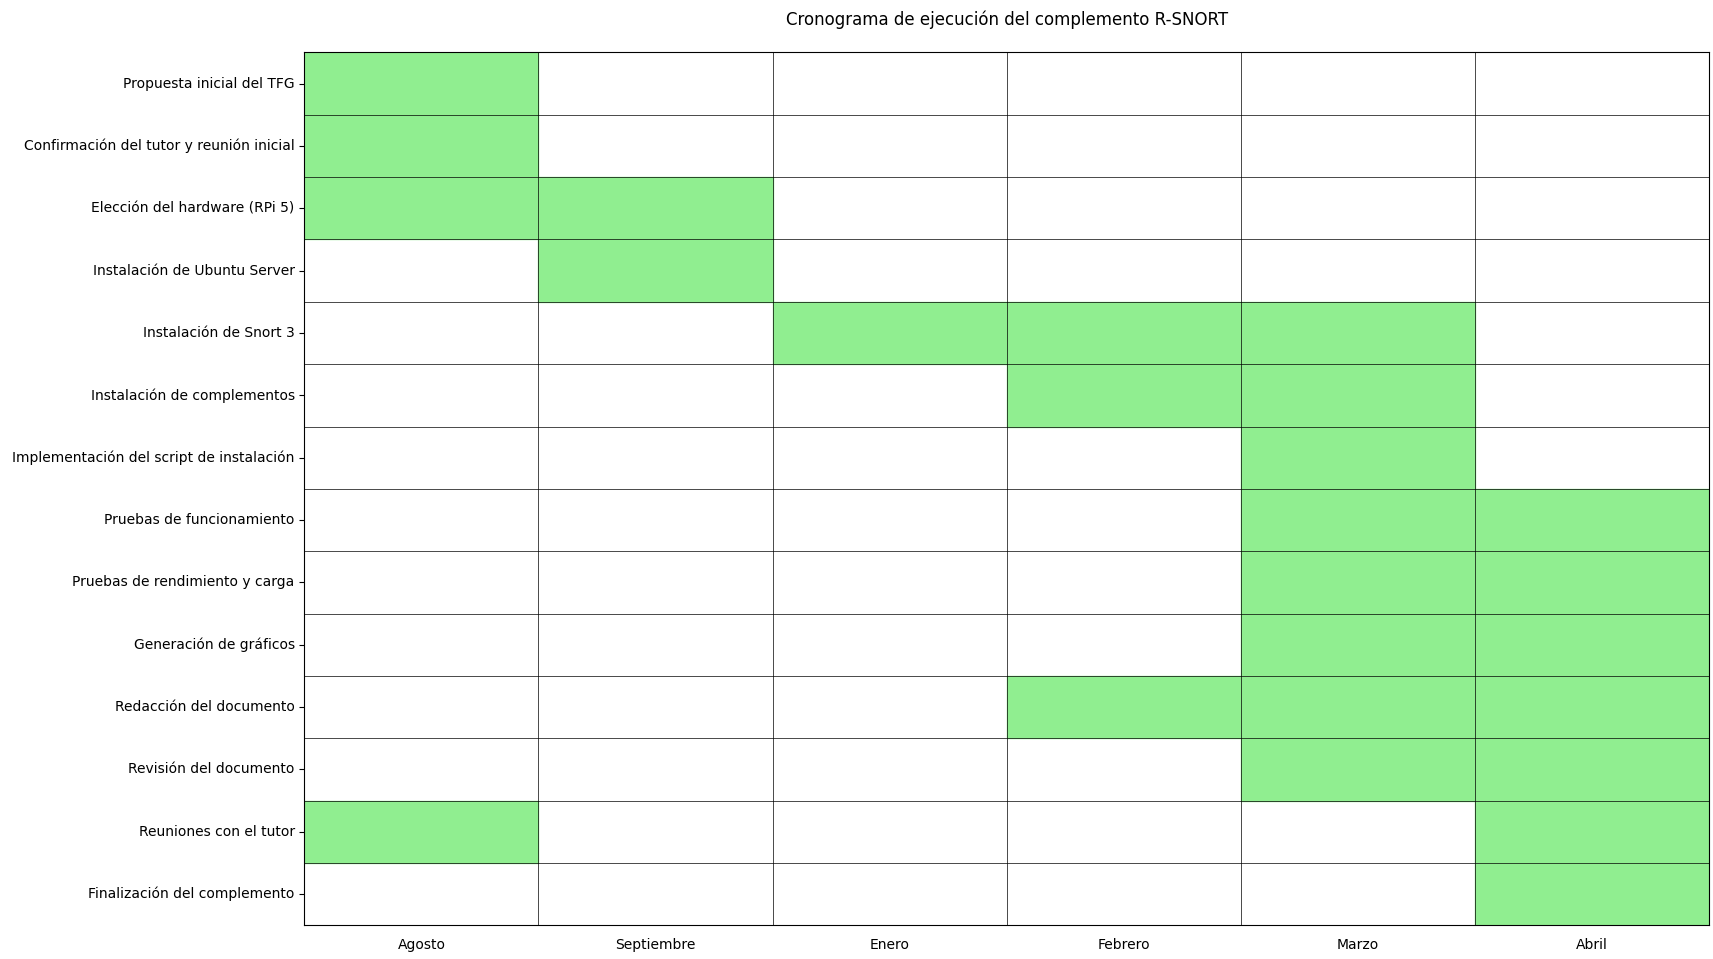
\includegraphics[scale=0.35]{cronograma/cronograma.png}
	\caption{Cronograma de las tareas.}
\end{figure}

\begin{figure}[H]
	\centering
	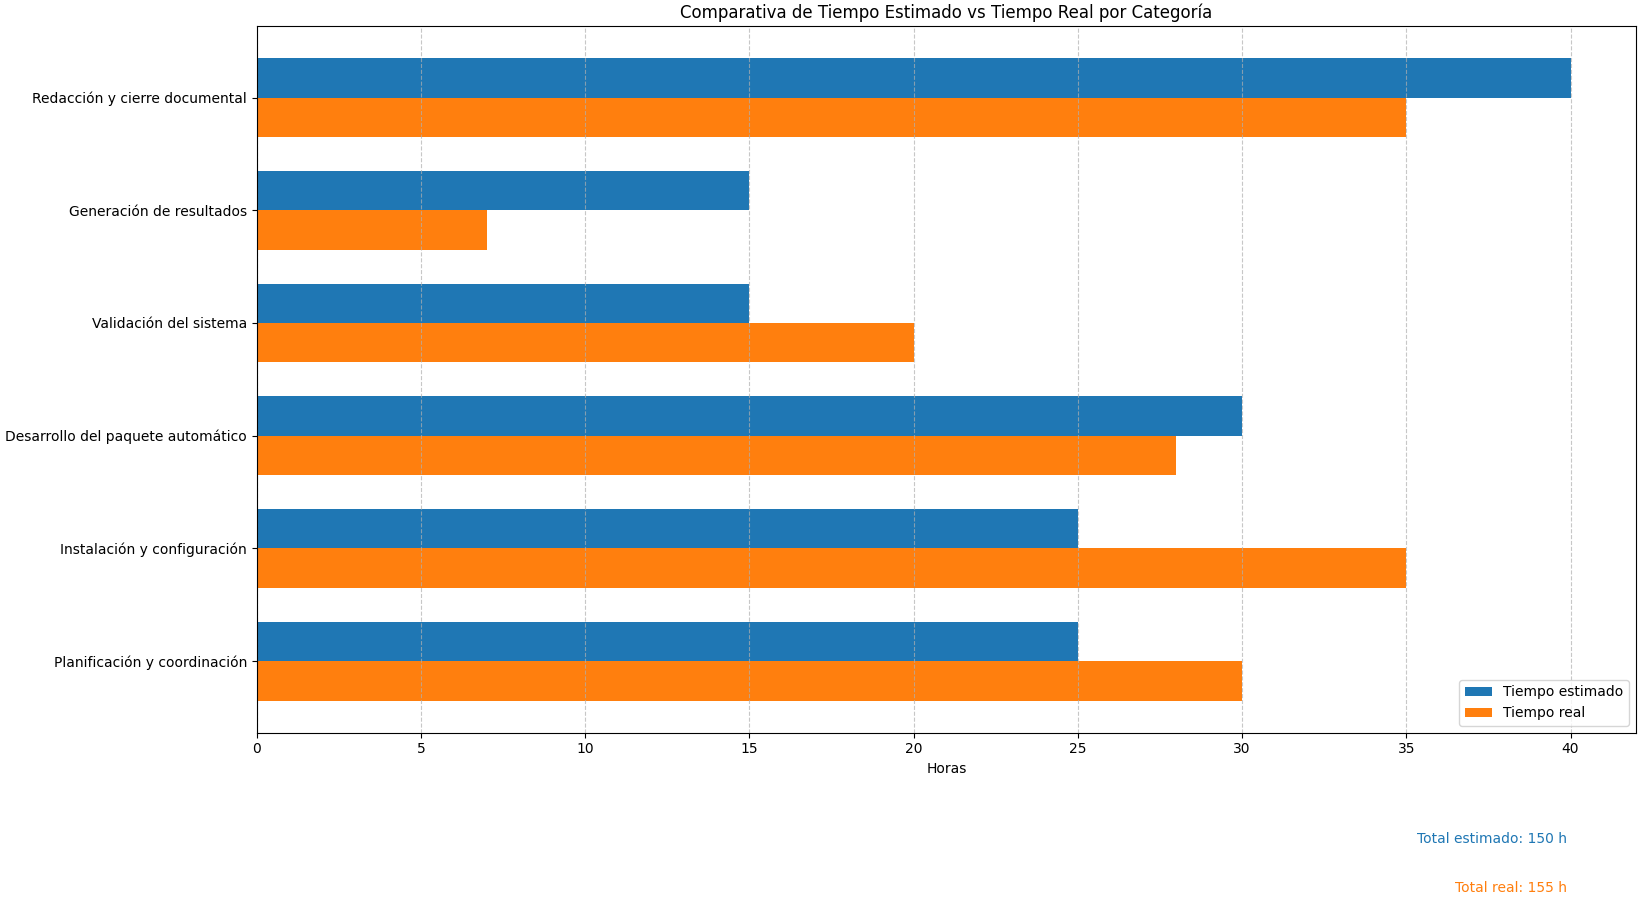
\includegraphics[scale=0.35]{cronograma/real_estimado.png}
	\caption{Comparación entre el tiempo estimado y el real.}
\end{figure}


\chapter{Estructura y metodología}

El enfoque seguido ha sido principalmente \textbf{empírico}, centrado en la construcción de un sistema funcional y su posterior optimización. La metodología puede resumirse en lo siguiente:

\begin{itemize}
	\item \textbf{Iteración y mejora continua:} En lugar de definir de antemano todos los componentes del sistema, se optó por una construcción \textit{modular} e \textit{incremental}. Esto ha permitido corregir errores tempranos, redefinir objetivos parciales y mejorar la \textbf{robustez} del sistema progresivamente.
	
	\item \textbf{Análisis de compatibilidad y adecuación:} Dado que el entorno de ejecución es una \textit{Raspberry Pi} con arquitectura \textit{ARM} y los sistemas en los que se planea el despliegue de este trabajo serán plataformas similares, fue necesario evaluar cuidadosamente la compatibilidad de las versiones de \textit{Snort} y sus dependencias. Este análisis condujo, por ejemplo, a descartar \textbf{Snort 3.7} por incompatibilidades con \textit{NUMA} y optar por \textbf{Snort 3.1.84} como versión estable.
	
	\item \textbf{Selección de componentes según el escenario:} Se priorizaron configuraciones, módulos y \textit{plugins} relevantes para proteger redes pequeñas, como las de una oficina doméstica (\textbf{SOHO}), descartando funciones innecesarias o incompatibles con \textit{Snort 3}. La selección se basó tanto en documentación oficial como en pruebas reales de rendimiento.
	
	\item \textbf{Automatización y accesibilidad:} Una parte importante del trabajo se centró en la creación de un sistema de instalación automática, lo más transparente posible para el usuario final. La \textit{modularización} de scripts y la documentación clara fueron el objetivo, pues se espera que el usuario no tenga un conocimiento demasiado técnico. Por ello, se ha tratado de automatizar cada proceso.
	
	\item \textbf{Evaluación empírica del rendimiento:} Finalmente, el sistema fue sometido a pruebas prácticas, midiendo el consumo de recursos con y sin \textit{Snort} activo. Los resultados fueron procesados mediante herramientas estadísticas y visualizados en forma de \textbf{gráficas generadas automáticamente}.
\end{itemize}

\pagebreak

\section*{Estructura del documento}

El documento se ha dividido en distintos puntos que pretenden ayudar al lector a seguir sin complicación el flujo de trabajo:

\begin{itemize}
	\item \textbf{Capítulos 1 al 4:} Introducen la motivación personal y los objetivos generales, junto con las fases de realización y la estructura del presente documento.
	
	\item \textbf{Capítulo 5:} Se exponen las principales funcionalidades, ventajas y explicación del comportamiento de los \textit{IDS}; posteriormente, se hace una introducción didáctica a \textit{Snort} como IDS.
	
	\item \textbf{Capítulo 6:} Este punto describe la utilización de un \textit{NIDS} en las redes objetivo. Se muestran las especificaciones de \textbf{Snort 3}, los requisitos de su instalación con sus \textit{preprocesadores} y configuración personalizada para \textbf{SOHO} \cite{cocsar2017firewall}, junto con la descripción de su transformación a \textit{script} automática para, finalmente, convertirse en un paquete automático \texttt{.deb}, que en esencia es el corazón de instalación de \textbf{R-Snort}.
	
	\item \textbf{Capítulo 7:} Casos prácticos de \textbf{R-Snort} funcionando en un entorno real como es una \textit{red doméstica}, puesta a prueba y evaluación del rendimiento.
	
	\item \textbf{Capítulo 8:} Finalizando el proyecto, se discuten los resultados obtenidos durante este trabajo.
	
	\item \textbf{Conclusiones:} Recoge las pruebas prácticas realizadas sobre el sistema, así como las gráficas de rendimiento obtenidas.
	
	\item Además se incluyen un resumen de resultados, conclusiones y anexos con información complementaria.
\end{itemize}

Esta estructura ha sido cuidadosamente diseñada para poder replicarse y adaptarse a otros entornos, contribuyendo así a la difusión de herramientas de seguridad accesibles.



\chapter{Sistemas de Detección de Intrusos}

\section{Los sistemas de detección de intrusos}

El objetivo de esta sección es mostrar una visión general de los Sistemas de Detección de Intrusos (IDS), su importancia en la seguridad informática y cómo encajan en el panorama actual de ciberseguridad.

\subsection{Definición y propósito de los IDS}

Un sistema de \textbf{Detección de Intrusos (IDS)} es una herramienta de \textit{ciberseguridad} que monitorea una red en busca de actividades anómalas o algún tipo de violación de políticas de seguridad, tanto del interior de la red como provenientes del exterior \cite{cichonski2012guide}.\newline

Su principal función es \textbf{detectar accesos no autorizados} y \textbf{comportamientos fuera de lo común} que, de alguna manera, puedan comprometer la \textbf{confidencialidad}, \textbf{integridad} o \textbf{disponibilidad} de los equipos.\newline

Mientras que un \textbf{IDS} se encarga de detectar y alertar sobre posibles intrusiones, un \textbf{Sistema de Prevención de Intrusos (IPS)} no solo detecta, sino que también toma medidas para \textbf{bloquear o prevenir dichas intrusiones en tiempo real} \cite{abbas2023ids}.

\subsection{Clasificación de los IDS}

\begin{itemize}
	\item \textbf{Según su ubicación}:
	\begin{itemize}
		\item \textbf{IDS basados en host (HIDS)}: Monitorizan y analizan la actividad interna de un sistema individual, revisando \textit{logs}, integridad de archivos y procesos en ejecución.
		
		\item \textbf{IDS basados en red (NIDS)}: Supervisan el tráfico de red en busca de actividades sospechosas, analizando los \textit{paquetes} que circulan por la red para detectar patrones de ataque.
	\end{itemize}
	
	\item \textbf{Según el tipo de datos que analizan}:
	\begin{itemize}
		\item \textbf{Basado en anomalias}: Buscan comportamientos fuera de lo común dentro de un sistema o red que puedan resultar sospechosos o malintencionados \cite{garcia2009anomaly}.
		
		\item \textbf{Basado en firmas}: Reconocen patrones previamente identificados, mediante bases de datos u otros métodos, para detectar comportamientos que coinciden con ciberataques conocidos o fugas de datos \cite{detection2005signature}.
	\end{itemize}
\end{itemize}


\subsection{Arquitectura y componentes de un IDS}

Un \textbf{IDS} generalmente cuenta con las siguientes partes:

\begin{itemize}
	\item \textbf{Sensores}: Estos son los encargados de capturar los datos provenientes de la red o del propio anfitrión.
	
	\item \textbf{Analizadores}: Se encargan de analizar y examinar los patrones en los paquetes recibidos en busca de coincidencias con comportamientos anómalos o firmas conocidas.
	
	\item \textbf{Bases de datos de firmas}: Almacenan patrones de ataques conocidos para la detección basada en firmas.
	
	\item \textbf{Interfaz de gestión}: Permite a los administradores configurar el sistema, revisar alertas y generar informes.
\end{itemize}

\subsection{Funcionalidades}

El sistema incorpora una serie de funcionalidades principalmente orientadas a la supervisión continua, la respuesta ante incidentes y la integración con otras herramientas de ciberseguridad.

\begin{itemize}
	\item \textbf{Monitorización en tiempo real}: Está siempre activo con el objetivo de captar cualquier tipo de intrusión de manera inmediata y poder actuar con rapidez.
	
	\item \textbf{Generación de alertas}: Por cada tipo de intrusión o sospecha, se genera un determinado tipo de alerta con descripciones relevantes para que de un rápido vistazo el administrador encargado pueda tomar acción rápidamente.
	
	\item \textbf{Registro de eventos}: Se documentan los incidentes ocurridos para posterior análisis forense y cumplimiento normativo, facilitando el trabajo del especialista que se encargue de un determinado ataque.
	
	\item \textbf{Integración con otros sistemas de seguridad}: Trabaja en conjunto con \textit{cortafuegos}, sistemas de gestión de eventos (\textbf{SIEM}), entre otras herramientas, con el objetivo de mejorar la defensa continuamente y estar preparados para amenazas posteriores.
\end{itemize}




\subsection{Ventajas y limitaciones de los IDS}

Como todo sistema de seguridad, los IDS tienen puntos fuertes y aspectos mejorables. A continuación se resumen sus principales ventajas y limitaciones:

\subsubsection{Ventajas}

\begin{itemize}
	\item Permiten detectar amenazas en etapas tempranas, lo que ayuda a responder antes de que causen daños.
	\item Mejoran la capacidad de reacción ante incidentes de seguridad.
	\item Facilitan el cumplimiento de normativas y ayudan en el análisis posterior de eventos.
\end{itemize}

\subsubsection{Limitaciones}

\begin{itemize}
	\item Pueden generar falsos positivos o no detectar ciertas amenazas.
	\item Requieren actualizaciones constantes para seguir siendo efectivos, y algunas opciones automáticas son de pago.
	\item Suponen un cierto consumo de recursos, aunque esto suele ser aceptable si se prioriza la seguridad.
\end{itemize}



\subsection{Contexto actual}

Con el incremento de amenazas avanzadas y persistentes (\textbf{APT}) \cite{cortes2017amenazas}, los \textbf{IDS} deben evolucionar incorporando \textit{inteligencia artificial} y \textit{aprendizaje automático} para mejorar la detección. Además, la integración con sistemas de gestión de información y eventos de seguridad (\textbf{SIEM}) es de especial interés para una respuesta coordinada y más eficaz.\newline

Ataques como el gusano \textit{SQL Slammer} en 2003 \cite{travis2004analysis} fueron detectados por \textit{IDS basados en firmas}, mientras que amenazas más sofisticadas, como \textit{Stuxnet} en 2010 \cite{kerr2010stuxnet} \cite{al2018stuxnet}, requirieron análisis más avanzados para su identificación. Comparaciones entre \textbf{HIDS} y \textbf{NIDS} en entornos específicos muestran que, aunque los HIDS ofrecen una visión detallada del host, los NIDS proporcionan una perspectiva más amplia del tráfico de red.

\section{Snort}

En esta sección se pretende profundizar en \textbf{Snort}\cite{snortweb} como uno de los \textbf{NIDS} más populares y versátiles, destacando sus características, funcionamiento y relevancia en entornos de seguridad.\newline

Desarrollado por Martin Roesch en 1998, Snort ha evolucionado hasta convertirse en un estándar en sistemas de detección de intrusiones de código abierto junto con otros detectores de intrusos como Suricata \cite{suricata_official}. En 2013, Cisco Systems adquirió Sourcefire, la empresa detrás de Snort, integrándolo en su portafolio de soluciones de seguridad. \textit{Snort} es utilizado en una amplia variedad de escenarios, desde pequeñas oficinas hasta grandes corporaciones y entornos educativos, gracias a su capacidad de adaptación. Puede identificar actividades maliciosas como inyecciones \textit{SQL}, escaneos de puertos y ataques de denegación de servicio (\textbf{DoS}), proporcionando alertas en tiempo real para una respuesta rápida. Tiene la capacidad de detectar casi cualquier tipo de actividad sospechosa gracias a las reglas creadas por la comunidad o por el propio administrador del sistema.

\subsection{Características principales}

Snort se distingue por algunas funciones que le permiten adaptarse a distintos escenarios y necesidades. Entre las más destacadas se encuentran:

\begin{itemize}
	\item \textbf{Motor de detección basado en firmas}: utiliza reglas predefinidas para detectar patrones de ataque conocidos.
	
	\item \textbf{Modos de operación}:
	\begin{itemize}
		\item \textbf{Sniffer}: Captura y muestra los paquetes de red en tiempo real.
		\item \textbf{Packet Logger}: Guarda los paquetes para analizarlos más adelante.
		\item \textbf{Network Intrusion Detection (NIDS)}: Examina el tráfico de red y lanza alertas si detecta actividad sospechosa.
		\item \textbf{Network Intrusion Prevention (IPS)}: Además de detectar tráfico malicioso, es capaz de bloquear o rechazar automáticamente paquetes peligrosos en tiempo real para prevenir intrusiones.
	\end{itemize}
\end{itemize}

\subsection{Arquitectura de Snort}

El funcionamiento de Snort se basa en una arquitectura modular, donde cada componente cumple un papel específico dentro del proceso de detección. Sus principales elementos son:

\begin{itemize}
	\item \textbf{Preprocesadores}: Adaptan el tráfico para su análisis, resolviendo fragmentaciones y otros detalles técnicos.
	\item \textbf{Motor de detección}: Compara el tráfico con las reglas definidas para identificar amenazas.
	\item \textbf{Plugins de salida}: Se encargan de registrar o enviar las alertas generadas, ya sea a archivos, bases de datos o servicios como syslog.
\end{itemize}

\begin{figure}[H]
	\centering
	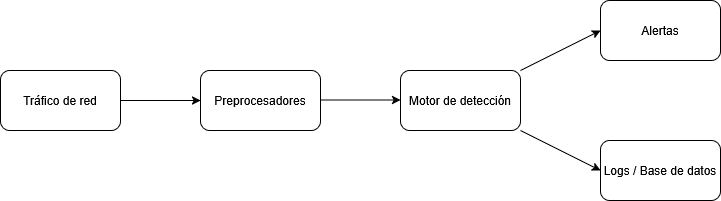
\includegraphics[scale=0.5]{adicional/diagrama_arquitectura.png}
	\caption{Arquitectura del funcionamiento de Snort.}
\end{figure}

\subsection{Reglas y actualizaciones}

\subsubsection{Estructura de una regla de Snort}

Una regla típica de \textbf{Snort} se compone de dos partes principales: el \textbf{encabezado} y las \textbf{opciones} \cite{snort3_rules_docs}. Por un lado, el encabezado define la acción a tomar (por ejemplo, alertar), el protocolo, las direcciones IP de origen y destino, y los puertos. Las opciones especifican condiciones adicionales, como patrones de contenido a buscar, mensajes de alerta y otros parámetros.

\begin{verbatim}
	alert tcp any any -> 192.168.1.0/24 80 (msg:"Posible acceso HTTP";
	 content:"GET"; sid:1000001; rev:1;)
\end{verbatim}

Esta regla genera una alerta si se detecta una conexión TCP desde cualquier origen hacia la red \texttt{192.168.1.0/24} en el puerto 80, y si el contenido del paquete contiene la cadena \texttt{"GET"}, típica de una solicitud HTTP. El campo \texttt{msg} define el mensaje de alerta, mientras que \texttt{sid} y \texttt{rev} son identificadores únicos para gestión y versiones.


\subsubsection{Tipos de reglas}

Snort utiliza distintos conjuntos de reglas que varían en disponibilidad, frecuencia de actualización y nivel de protección. Los tipos principales son:

\begin{itemize}
	\item \textbf{Community Rules}: Reglas creadas y mantenidas por la comunidad de usuarios de \textit{Snort}, disponibles de forma gratuita bajo la licencia \textit{GPLv2}.
	
	\item \textbf{Registered Rules}: Proporcionadas por \textit{Cisco Talos}, disponibles para usuarios registrados, aunque con un retraso de 30 días respecto al lanzamiento para suscriptores.
	
	\item \textbf{Subscriber Rules}: Reglas actualizadas en tiempo real, pensadas para usuarios de pago. Ofrecen protección frente a amenazas emergentes sin retrasos \cite{snort_talos} (\textit{no usadas en este proyecto}).
\end{itemize}


\subsubsection{Gestión de reglas}

Herramientas como \textit{PulledPork} y \textit{Oinkmaster} facilitan la descarga, actualización y gestión de las reglas de \textit{Snort}, automatizando procesos y asegurando que el sistema esté protegido contra las últimas amenazas.

\subsection{Personalización y extensibilidad}

\subsubsection{Creación de reglas personalizadas}

Los administradores pueden desarrollar reglas específicas adaptadas a las necesidades particulares de su entorno, permitiendo una detección más precisa de amenazas relevantes para su organización.

\subsubsection{Uso de variables y listas}

\textit{Snort} permite definir variables para representar direcciones IP, rangos de puertos y otras configuraciones, facilitando la gestión y actualización de las reglas.

\subsubsection{Integración con otros sistemas}

\textit{Snort} puede integrarse con herramientas como \textit{Barnyard2}, \textit{Snorby} y \textit{Sguil} para mejorar la gestión de alertas, análisis de eventos y generación de informes.

\subsection{Limitaciones y consideraciones}

\subsubsection{Rendimiento en redes de alta velocidad}

En entornos con tráfico de red intenso, es una necesidad prioritaria contar con \textbf{hardware adecuado} y una \textbf{configuración óptima} para asegurar que \textit{Snort} funcione correctamente sin afectar el rendimiento del sistema.

\subsubsection{Gestión de falsos positivos}

La tarea de ajustar y afinar las reglas para minimizar las alertas falsas es prioritaria, evitando así una sobrecarga de información y permitiendo a los administradores centrarse en amenazas reales.

\section{Necesidades de seguridad en pequeñas redes (SOHO)}

Se pretende analizar las necesidades específicas de seguridad en redes pequeñas, como oficinas domésticas o pequeñas empresas (\textbf{SOHO}), y cómo soluciones como \textit{Snort} pueden ser implementadas eficientemente.\newline

Las redes \textbf{SOHO} suelen estar compuestas por un número reducido de dispositivos y recursos limitados, y a menudo carecen de personal especializado en \textit{TI}. A pesar de su tamaño, estas redes juegan un papel importante para la economía y requieren medidas de seguridad adecuadas \cite{ruedarevisiting}.

\subsection{Amenazas y vulnerabilidades comunes}

Toda red, por pequeña que sea, está expuesta a distintos tipos de amenazas. Algunas vienen del exterior, otras desde dentro, y muchas están relacionadas con dispositivos mal configurados. A continuación se describen las más relevantes:

\subsubsection{Amenazas externas}

Incluyen el uso de \textit{malware}, ataques de \textit{phishing} y fuerza bruta contra servicios accesibles desde Internet.

\subsubsection{Amenazas internas}

Pueden deberse a un mal uso de los recursos, conexiones inseguras desde dispositivos personales o la falta de normas claras sobre seguridad en la red.

\subsubsection{Dispositivos IoT}

El crecimiento del número de dispositivos conectados (como cámaras, sensores o dispositivos \textit{wearables}) supone un riesgo añadido. Entre los problemas más frecuentes se encuentran:

\begin{itemize}
	\item Uso de credenciales por defecto que no pueden cambiarse.
	\item Comunicación sin cifrado, como en versiones inseguras de MQTT.
	\item Falta de actualizaciones o mantenimiento del firmware \cite{bakhshi2024review}.
\end{itemize}


Una solución práctica es implementar segmentación de red mediante VLANs para aislar estos dispositivos, combinado con reglas específicas en \textit{Snort 3} para monitorizar tráfico en puertos comunes IoT (ej: 1883 para MQTT, 5683 para CoAP).

\subsection{Retos específicos}

\subsubsection{Limitaciones de recursos}

Al tratarse de una solución orientada a entornos pequeños, optimizar el consumo de recursos pertenece a la lista de objetivos principales. Para ello, se aplican medidas como:

\begin{itemize}
	\item Uso de hardware eficiente como la \textit{Raspberry Pi 5}, con un consumo inferior a 10W.
	\item Empleo de reglas gratuitas, como las de \textit{Emerging Threats Open}.
	\item Configuraciones predefinidas en \textit{Snort 3} enfocadas a detectar amenazas críticas.
\end{itemize}

Además, la versión 3 de Snort introduce un motor multi-hilo que mejora el rendimiento en sistemas con pocos recursos, gracias a un procesamiento más selectivo del tráfico \cite{park2017performance}.


\subsubsection{Conectividad constante}
Estrategias de mitigación:
\begin{itemize}
	\item Inspección de tráfico VPN (\textit{WireGuard/OpenVPN}) mediante preprocesadores de \textit{Snort}.
	\item Reglas específicas para detección de ataques a servicios RDP/SSH.
	\item Integración con sistemas de autenticación multifactor para acceso remoto.
\end{itemize}

\subsection{Soluciones adecuadas para redes SOHO}

En entornos pequeños o domésticos, la seguridad debe abordarse por capas. A continuación se describe lo que debería incluir una posible configuración mínima:

\begin{itemize}
	\item Cortafuegos basado en \texttt{iptables} con políticas restrictivas por defecto.
	\item Integración de un \textit{antivirus de red}, como \textit{ClamAV}, para inspeccionar tráfico sospechoso.
	\item Mecanismos de actualización automática mediante repositorios firmados digitalmente.
\end{itemize}

Las pequeñas oficinas o entornos domésticos SOHO suelen contar con presupuestos limitados y pocos recursos técnicos. En estos casos, el uso de soluciones de código abierto es una alternativa muy viable por su bajo coste y flexibilidad.

\subsubsection{Herramientas de código abierto}

Optar por software libre tiene múltiples beneficios:

\begin{itemize}
	\item \textbf{Comunidades activas} que mantienen más de 500 reglas actualizadas mensualmente en herramientas como \textit{Snort}.
	\item \textbf{Compatibilidad multiplataforma}, lo que facilita su uso en distintos dispositivos y sistemas operativos.
	\item \textbf{Auditoría del código fuente}, que permite identificar vulnerabilidades o errores de seguridad antes de que sean explotados.
\end{itemize}


\subsubsection{Dispositivos de bajo coste}

Una solución económica y funcional puede construirse sobre una \textit{Raspberry Pi 5} con:

\begin{itemize}
	\item Un sistema operativo seguro, como \textit{Ubuntu Server LTS}, \textit{Raspbian OS} o \textit{Debian}.
	\item Supervisión de parámetros físicos: temperatura, voltaje y consumo energético.
\end{itemize}

%{Servicios gestionados}

%Una estrategia híbrida permite combinar simplicidad con eficacia:

%\begin{itemize}
%	\item \textit{Detección local} mediante \textit{Snort} en la Raspberry Pi.
%	\item \textit{Respuesta automatizada básica}, como el bloqueo de IPs mediante una API de cortafuegos.
%\end{itemize}

%Este enfoque equilibra costes y protección, utilizando capacidades reales de \textit{Snort 3} y hardware accesible, sin necesidad de grandes inversiones ni personal técnico dedicado.

\section{Beneficios y recomendaciones de los sistemas de detección en redes reducidas}

Implementar un sistema de detección en redes pequeñas ofrece múltiples ventajas:

\begin{itemize}
	\item \textbf{Identificación preventiva de riesgos}: La monitorización continuo permite detectar comportamientos sospechosos a tiempo, mejorando la capacidad de respuesta.
	\item \textbf{Análisis del tráfico de red}: Facilita auditorías internas al observar cómo se comunican los dispositivos entre sí, ayudando a detectar puntos débiles.
	\item \textbf{Cumplimiento de normativas de seguridad}: Aporta trazabilidad y evidencia para cumplir con protocolos básicos de protección de datos.
\end{itemize}

%\section{Prácticas recomendadas de seguridad para entornos SOHO}

Por otro lado para mejorar la seguridad general en redes pequeñas, se recomienda adoptar las siguientes medidas:

\begin{itemize}[itemsep=6pt]
	\item \textbf{Autenticación reforzada}: Emplear contraseñas robustas, que incluyan símbolos, números, mayúsculas y minúsculas, y actualizarlas periódicamente. Evitar datos personales o corporativos.
	
	\item \textbf{Segmentación de red}: Dividir la red en zonas lógicas para contener posibles incidentes y limitar la propagación en caso de intrusión.
	
	\item \textbf{Copias de seguridad}: Automatizar el respaldo de datos críticos para garantizar su recuperación ante fallos o ataques.
	
	\item \textbf{Monitorización y detección de intrusos}: Implementar sistemas que permitan vigilar el tráfico de red y detectar actividades anómalas en tiempo real. El uso de un IDS (Sistema de Detección de Intrusos) constituye una defensa activa en redes SOHO. Como ejemplo, \textit{Snort 3} ofrece funciones de inspección profunda de paquetes, entre las que se incluyen la detección de patrones en protocolos de aplicación (HTTP, DNS, FTP), y el soporte nativo para formatos modernos como \textit{JSON} y \textit{HTTP/2}.
\end{itemize}

\section{Complementos y plugins para Snort}

Snort 3 adopta una arquitectura modular que permite activar o desactivar complementos según las necesidades de cada entorno. Esto resulta especialmente útil en entornos de recursos limitados como una Raspberry Pi (o cualquier otro sistema similar), donde es necesario encontrar un equilibrio entre capacidad de inspección y rendimiento. En el caso de R-SNORT, se han seleccionado e integrado los módulos más relevantes para proteger la red de una PYME sin comprometer la estabilidad del sistema.\newline

A continuación, se detallan los complementos activados y configurados en el archivo, agrupados por su funcionalidad:

\begin{itemize}
	\item \textbf{Inspección de protocolos a nivel de aplicación:}  
	\textbf{R-SNORT} incorpora múltiples plugins para analizar protocolos de red en profundidad. Entre ellos destacan:
	\begin{itemize}
		\item \textbf{HTTP y HTTP2 (\texttt{http\_inspect}):} Permiten la inspección completa de peticiones y respuestas, incluyendo cabeceras, URIs y cuerpos comprimidos, así como la detección de estructuras anómalas como cabeceras sobredimensionadas o URIs malformadas.
		\item \textbf{DNS, SMTP, FTP, SSH, SIP, Telnet, POP3, IMAP, SSL/TLS:} Cada uno gestionado por su módulo correspondiente, para detectar comportamientos sospechosos y ataques comunes como \textit{exfiltración de datos}, \textit{tunneling} o abuso de protocolos.
	\end{itemize}
	
	\item \textbf{Inspección de flujos y reensamblado:}  
	La configuración activa los módulos modernos de \textbf{Snort 3} para gestionar flujos de red:
	\begin{itemize}
		\item \textbf{Stream IP y Stream TCP:} Sustituyen a los antiguos \texttt{frag3} y \texttt{stream5}. Se encargan del reensamblado de fragmentos IP y sesiones TCP, previniendo técnicas de evasión mediante solapamiento de paquetes o sesiones incompletas.
		\item \textbf{Configuraciones de timeout, solapamientos, fragmentos pequeños y límites de sesión:} Estos parámetros han sido ajustados específicamente para mantener un buen rendimiento en entornos embebidos, sin comprometer la seguridad.
	\end{itemize}
	
	\item \textbf{Reputación IP y listas negras (\texttt{reputation}):}  
	\textbf{R-SNORT} integra un sistema de reputación básico que permite bloquear IPs listadas en un archivo de tipo \texttt{blocklist.rules}. Esta funcionalidad es útil para prevenir conexiones hacia o desde dominios maliciosos previamente identificados.
	
	\item \textbf{Soporte para protocolos industriales:}  
	Aunque no todos están activos simultáneamente, el sistema tiene soporte habilitado para protocolos comunes en entornos industriales como \texttt{Modbus}, \texttt{DNP3}, \texttt{S7CommPlus}, \texttt{CIP} o \texttt{IEC 104}. Esto permitiría adaptar \textbf{R-SNORT} a una red \textit{OT (Operational Technology)} con muy pocos cambios.
	
	\item \textbf{Integración con antivirus (ClamAV):}  
	Aunque no se encuentra directamente gestionado desde el archivo de configuración de Snort, el sistema está preparado para trabajar conjuntamente con \textbf{ClamAV} mediante scripts de análisis de tráfico o detección de amenazas basada en archivos. Esta funcionalidad complementa a Snort para detectar \textit{malware} en transmisiones de red.
	
	\item \textbf{Inspección de tráfico cifrado y evasión SSL (\texttt{ssl}):}  
	El módulo de SSL permite detectar y registrar ciertos ataques conocidos como \textit{Heartbleed}, estableciendo límites de tamaño en los mensajes \texttt{heartbeat} y controlando el comportamiento anómalo de certificados.
	
	\item \textbf{Inspección de archivos y tipos MIME:}  
	Aunque se ha desactivado la descompresión de formatos complejos como PDF o ZIP por motivos de rendimiento, el sistema conserva capacidades básicas de inspección de archivos mediante los módulos \texttt{file\_id} y \texttt{file\_policy}, útiles para reglas que dependan del tipo de archivo transmitido.
\end{itemize}

Cabe destacar que \textbf{Snort 3} ya no utiliza el formato de salida \texttt{Unified2}, por lo que herramientas como \textbf{Barnyard2} no son compatibles \cite{snort_gui_update}. En su lugar, \textbf{R-SNORT} se apoya en registros en texto plano y en el análisis posterior mediante un sistema de visualización web personalizado.

% Continúa con el resto de capítulos y secciones siguiendo la estructura
\chapter{Utilización de Snort en redes SOHO}
\section{Introducción}

Un Sistema de Detección de Intrusos en la Red (NIDS, por sus siglas en inglés) es una herramienta de seguridad que permite la monitorización del tráfico en busca de actividades sospechosas o ataques que coincidan con patrones conocidos. En el contexto de pequeñas redes, como las de hogares o pequeñas oficinas (SOHO), un NIDS puede representar una primera línea de defensa sin recurrir a costosas soluciones empresariales, favoreciendo así una ciberseguridad asequible para PYMES y usuarios particulares.\newline

En este proyecto se ha desarrollado e instalado R-Snort, una solución basada en Snort versión 3 junto con varios complementos, sobre una Raspberry Pi 5 con Ubuntu Server. Esta plataforma de bajo consumo y coste reducido ha demostrado ser suficientemente robusta para tareas avanzadas de inspección de tráfico, gracias a mecanismos como el \textit{port mirroring}, el uso del modo promiscuo y su despliegue como servicios. La construcción modular del sistema y su empaquetado en formato \texttt{.deb} han permitido una instalación automatizada, simplificando su adopción incluso por usuarios con escasos conocimientos técnicos.\newline

Durante las pruebas realizadas, se ha observado que el impacto en el rendimiento del sistema es bajo y controlado. Mediante herramientas profesionales de monitorización como \texttt{pmchart}, se han obtenido gráficas que reflejan un uso moderado de la CPU y la memoria, así como un aumento predecible en la escritura de disco en función de la actividad de red. Bajo condiciones normales, el sistema permanece mayoritariamente inactivo, con una actividad mínima centrada en el análisis de paquetes y la generación de logs. En escenarios de tráfico masivo inducido con \texttt{iperf3}, Snort mostró un comportamiento estable, con un incremento visible en la carga del sistema, pero sin llegar a comprometer su operatividad ni generar cuellos de botella críticos.\newline

En cuanto a la detección, R-Snort logró identificar múltiples tipos de tráfico potencialmente malicioso, incluyendo escaneos de puertos, anomalías en protocolos como ICMP y DNS, así como transmisiones de datos sensibles. Las alertas generadas fueron coherentes con las reglas definidas, tanto comunitarias como personalizadas. Aunque las pruebas se realizaron en un entorno controlado, los resultados obtenidos permiten anticipar una buena capacidad de detección en redes reales, siempre que se realicen los ajustes oportunos a las reglas y umbrales de alerta.\newline

Finalmente, se ha puesto especial énfasis en la usabilidad y el mantenimiento del sistema. La experiencia de usuario ha sido positiva gracias a un instalador modular, claro y autónomo, que permite desplegar R-Snort sin necesidad de configuraciones manuales complejas. Esta accesibilidad ha sido un objetivo clave para facilitar su implementación en entornos SOHO, donde no siempre se cuenta con personal técnico especializado.\newline

En conjunto, este trabajo demuestra que trasladar capacidades de detección de intrusos a dispositivos compactos y asequibles no solo es viable, sino también eficaz, contribuyendo a democratizar la seguridad en redes domésticas y de pequeña escala.


\section{Especificaciones, características y requisitos}

\subsection{Especificaciones de Snort 3}

Snort 3 es una versión mejorada de su predecesor, con una arquitectura modular y mejoras significativas en rendimiento y configuración. Algunas de sus características incluyen:

\begin{itemize}
\item \textbf{Arquitectura modular}: Permite una configuración flexible y personalizable apoyada por una gran cantidad de documentación.
\item \textbf{Mejoras en rendimiento}: Optimizaciones en el motor de detección para un procesamiento más eficiente.
\item \textbf{Soporte para multihilo}: Permite el uso de múltiples procesadores para mejorar el rendimiento en sistemas modernos.
\item \textbf{Reglas en Lua}: Facilita una configuración más avanzada y personalizable.
\item \textbf{Integración con DAQ (Data Acquisition Library)}: Ofrece opciones flexibles para la captura de paquetes en la red.
\item \textbf{Compatibilidad con reglas de Snort 2}: Permite utilizar reglas preexistentes.
\end{itemize}

\subsection{Requisitos del sistema}

Para garantizar el correcto funcionamiento de Snort en su versión 3, especialmente en entornos donde se emplean múltiples preprocesadores como \textit{daq}, \textit{appid}, \textit{file\_inspect}, \textit{http\_inspect} o el preprocesador \textit{SSL/TLS} entre otros, es importante que el sistema anfitrión cumpla con una serie de requisitos mínimos. No obstante, se recomienda ir más allá de estas especificaciones si se desea un rendimiento fluido y una capacidad de respuesta adecuada ante flujos de tráfico moderados o elevados.\newline

A continuación, se detallan los requisitos mínimos y recomendados para la instalación y operación estable de Snort 3.1.84, especialmente en entornos de tipo laboratorio o pequeñas redes empresariales.

\subsection*{Requisitos mínimos}

\begin{itemize}
	\item \textbf{Sistema operativo:} Linux (preferiblemente Ubuntu Server 20.04 LTS o superior, o CentOS 7+, Debian)
	\item \textbf{Arquitectura:} x86\_64 o ARMv8 (Raspberry Pi compatible, con limitaciones)
	\item \textbf{CPU:} Procesador de 2 núcleos a 1.5 GHz
	\item \textbf{Memoria RAM:} 2 GB
	\item \textbf{Almacenamiento libre:} 4 GB
	\item \textbf{Conectividad de red:} Interfaz Ethernet o Wi-Fi dedicada
	\item \textbf{Dependencias básicas:} \texttt{CMake (3.5+)}, \texttt{GCC (6.0+)}, \texttt{libpcap-dev}, \texttt{libpcre}, \texttt{zlib}, \texttt{OpenSSL}, \texttt{LuaJIT}, \texttt{libdnet}, entre otros.
\end{itemize}

\subsection*{Requisitos recomendados}

\begin{itemize}
	\item \textbf{Sistema operativo:} Ubuntu Server 22.04 LTS
	\item \textbf{CPU:} 4 núcleos a 2.5 GHz o superior
	\item \textbf{Memoria RAM:} 8 GB
	\item \textbf{Almacenamiento libre:} 20 GB
	\item \textbf{Interfaz de red dedicada:} Tarjeta de red exclusiva en modo promiscuo
	\item \textbf{Extra:} Desactivar NUMA en arquitecturas embebidas como Raspberry Pi.
\end{itemize}

\section{Entorno de trabajo}

El entorno de trabajo define los componentes físicos y lógicos involucrados en la implementación del NIDS con Snort 3. Para estructurar este apartado, se consideran los siguientes elementos:

\subsection{Esquema de red}

El esquema de red presente en el desarrollo del trabajo está compuesto por un \textbf{router doméstico}, un \textbf{switch gestionable} que permite \textit{port mirroring} hacia el puerto de \textbf{R-SNORT}. De esta manera, no se produce latencia ya que no es necesario interponer el proyecto entre la red local de máquinas y el router, desarrollándose así las comunicaciones con la fluidez habitual del sistema, junto a otros dos equipos que más adelante servirán para las pruebas de \textbf{detección de intrusos} y de \textbf{rendimiento}. La \textbf{Raspberry Pi} cuenta con dos interfaces \textit{ethernet}: la interfaz \texttt{enxc8a362b4a702}, proporcionada por un adaptador externo, será la encargada de recoger el \textbf{tráfico total de la red}, y la interfaz predeterminada \texttt{eth0}, que será la encargada de suministrar \textbf{acceso a internet} a la Raspberry Pi.

\begin{figure}[H]
	\centering
	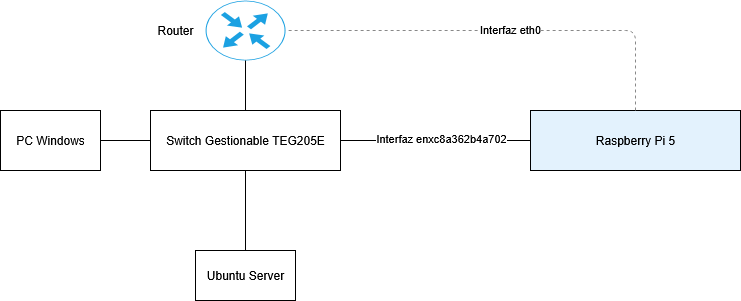
\includegraphics[scale=0.6]{script_automatico/network.png}
	\caption{Esquema de red real del proyecto.}
\end{figure}

\subsubsection*{Descripción del esquema}

La red está compuesta por:

\begin{itemize}
	\item Un \textbf{switch gestionable} (modelo \texttt{Tenda TEG205E}) con capacidad de \textit{Port Mirroring}.
	\item Dos dispositivos cliente conectados a los puertos 2 y 3 del switch: un ordenador con \textbf{Windows} y una máquina con \textbf{Ubuntu Server}.
	\item Un \textbf{router doméstico} conectado al puerto 1 del switch, encargado de proporcionar acceso a Internet.
	\item Una \textbf{Raspberry Pi 5} equipada con dos interfaces de red Ethernet:
	\begin{itemize}
		\item \texttt{eth0}: Conectada directamente al router, proporciona conectividad a Internet para la propia Raspberry Pi.
		\item \texttt{enxc8a362b4a702}: Conectada al puerto 4 del switch, el cual está configurado como puerto espejo.
	\end{itemize}
\end{itemize}

\subsection{Hardware (Raspberry Pi 5)}

La \textbf{Raspberry Pi 5} se utiliza como base para la implementación del \textit{NIDS} debido a su bajo consumo energético y su potencia suficiente para analizar tráfico de red en pequeños entornos. Sus características principales incluyen:

\begin{itemize}
	\item \textbf{CPU}: ARM Cortex-A76 (4 núcleos a 2.4 GHz)
	\item \textbf{GPU}: VideoCore VII
	\item \textbf{RAM}: Modelos de 8\,GB LPDDR4X
	\item \textbf{Conectividad}:
	\begin{itemize}
		\item 2 puertos USB 3.0
		\item 2 puertos USB 2.0
		\item 1 puerto Ethernet Gigabit
		\item WiFi 802.11ac y Bluetooth 5.0 (\textit{deshabilitados por seguridad})
	\end{itemize}
	\item \textbf{Almacenamiento}:
	\begin{itemize}
		\item MicroSD de 32\,GB
		\item Soporte para SSD a través de USB 3.0
	\end{itemize}
\end{itemize}

\subsection{Software (Snort y sus complementos)}
\textbf{Snort 3} es un sistema de prevención y detección de intrusos en la red (\textit{NIDS/NIPS}) que introduce una serie de mejoras significativas sobre sus versiones anteriores, incluyendo mayor eficiencia, modularidad y una arquitectura basada en plugins. Estas mejoras hacen que \textbf{Snort 3} sea más \textit{adaptable, eficiente y personalizable} \cite{snort3_vs_snort2}.

\subsubsection{Comparación con Snort 2}
Snort 3 introduce una serie de mejoras sobre Snort 2:
\begin{itemize}
	\item Configuración más flexible y simplificada.
	\item Mayor rendimiento gracias al uso de múltiples hilos.
	\item Soporte para más de 200 plugins que permiten ampliar su funcionalidad.
	\item Sistema de reglas más eficiente y simplificado.
	\item Mejora en la detección de amenazas emergentes y reducción de falsos positivos.
\end{itemize}

\subsubsection{Plugins y complementos utilizados}
Para potenciar las capacidades de detección de \textbf{Snort 3} en este proyecto, se han seleccionado los siguientes \textit{preprocesadores} y herramientas adicionales:

\begin{itemize}
	\item \textbf{HTTP Inspect:} Analiza tráfico HTTP/HTTPS para detectar ataques \textit{SQL/XSS} e irregularidades en los encabezados.
	\item \textbf{SSL/TLS:} Inspecciona metadatos del tráfico cifrado y detecta conexiones sospechosas o anómalas.
	\item \textbf{Stream IP:} Ensambla paquetes IP fragmentados para detectar intentos de evasión.
	\item \textbf{Stream TCP:} Reensambla flujos TCP/UDP para un análisis más preciso.
	\item \textbf{Reputation Preprocessor:} Bloquea tráfico de fuentes maliciosas basado en listas de reputación. 
	\item \textbf{Conjunto de reglas de datos sensibles:} Detecta información sensible como números de tarjetas de crédito o credenciales expuestas.
	\item \textbf{ClamAV:} Sistema antivirus de código abierto que complementa la detección de amenazas de Snort con análisis basado en firmas.
\end{itemize}


\newpage

\section{Instalación y personalización de complementos}
\subsection{Instalación de Snort V3}
% Contenido de la sección 2.4

\subsubsection*{Preparación del entorno}

El desarrollo de lo que será \textbf{R-SNORT} empezará con la instalación de \textbf{Snort} \cite{snort3_installation_pdf} mismo en su versión actual. Para ello, es buena práctica actualizar los repositorios y el equipo mediante un \texttt{update} y un \texttt{upgrade} antes de comenzar la instalación. Una vez hecho esto, empezaremos con la instalación de las distintas librerías y dependencias de \textbf{Snort V3}.

\begin{lstlisting}
	$ sudo apt-get update && sudo apt-get upgrade -y
\end{lstlisting}

\subsubsection*{Instalación y configuración de \texttt{libdnet}}

Primero, instalamos un par de herramientas necesarias (\texttt{libtool} y \texttt{autoconf}) para compilar Snort 3. Luego, nos movemos al directorio \texttt{/usr/local/src} y clonamos el repositorio de \texttt{libdnet} desde GitHub, que es una librería importante para que Snort funcione correctamente. Finalmente, entramos en el directorio \texttt{libdnet} para seguir con la instalación.

\begin{figure}[H]
	\centering
	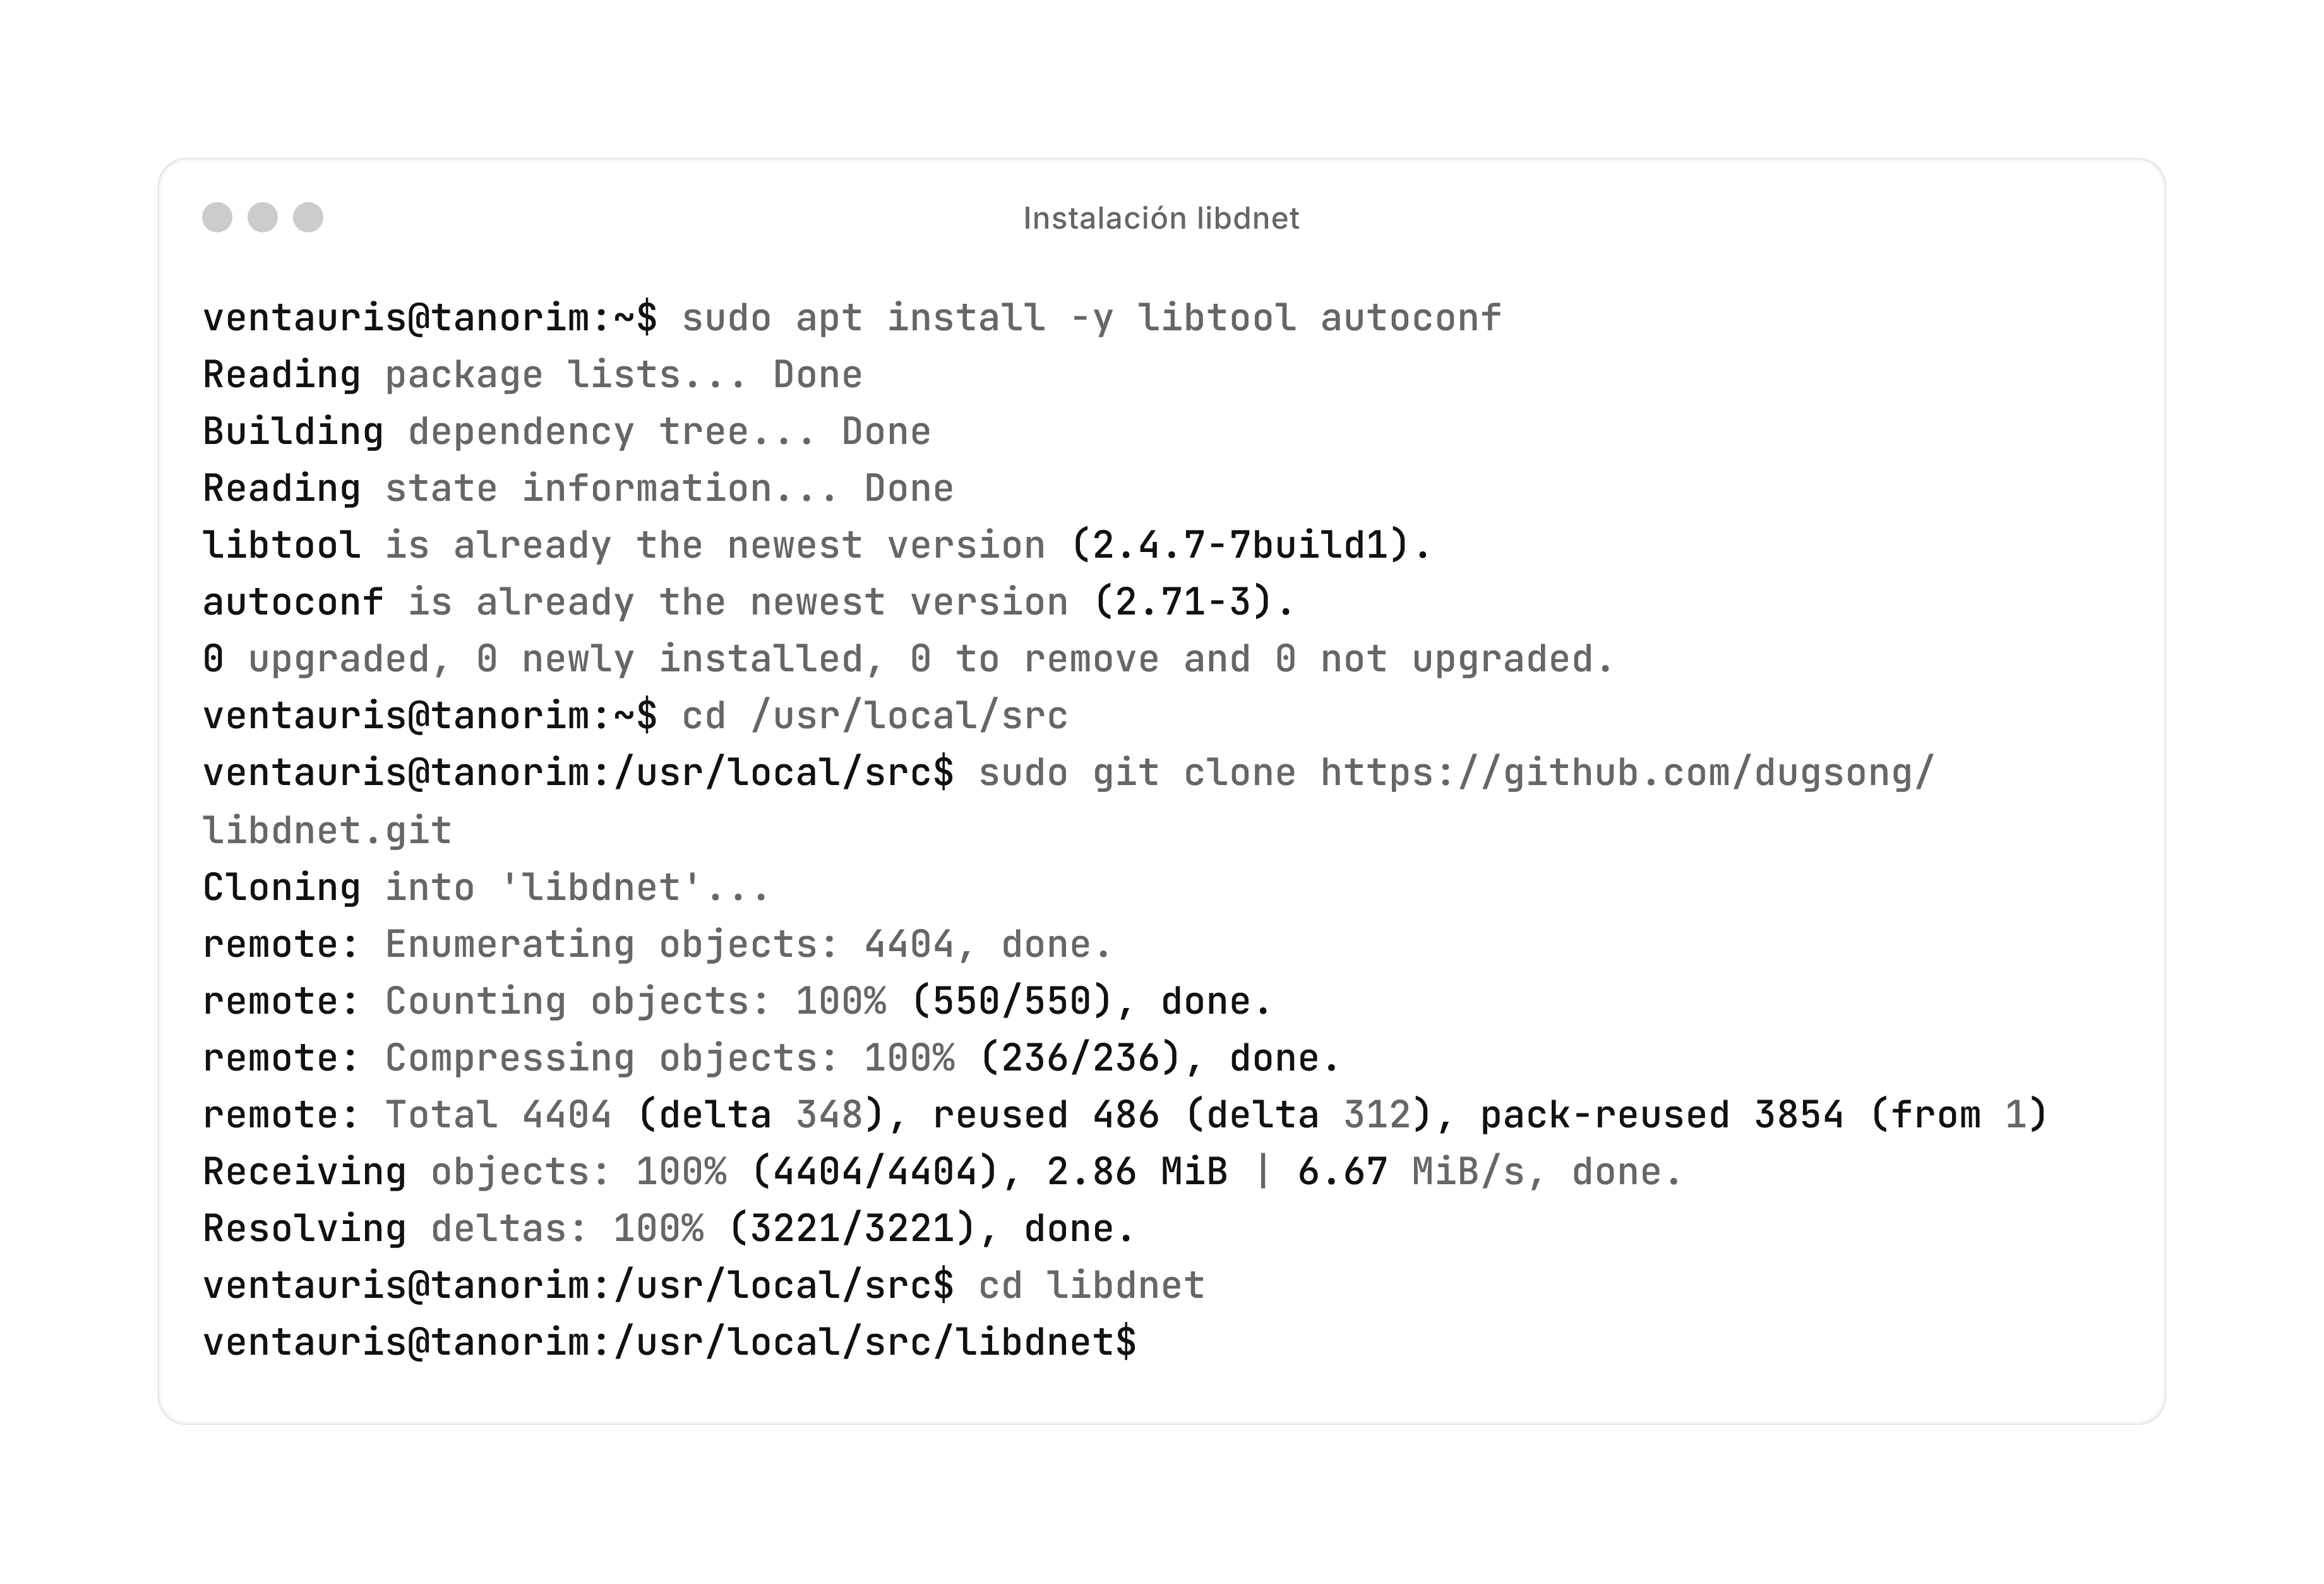
\includegraphics[scale=0.12]{instalacion_snort/1-1.png}
	\caption{Instalando dependencias necesarias.}
\end{figure}

\newpage

A continuación, el paquete \texttt{check} es instalado. Esta herramienta servirá principalmente para ejecutar algunas pruebas en C. Es un requisito para poder compilar \texttt{libdnet} correctamente. Gracias a estas preparaciones, estamos configurando el entorno para la correcta compilación de Snort.

\begin{figure}[H]
	\centering
	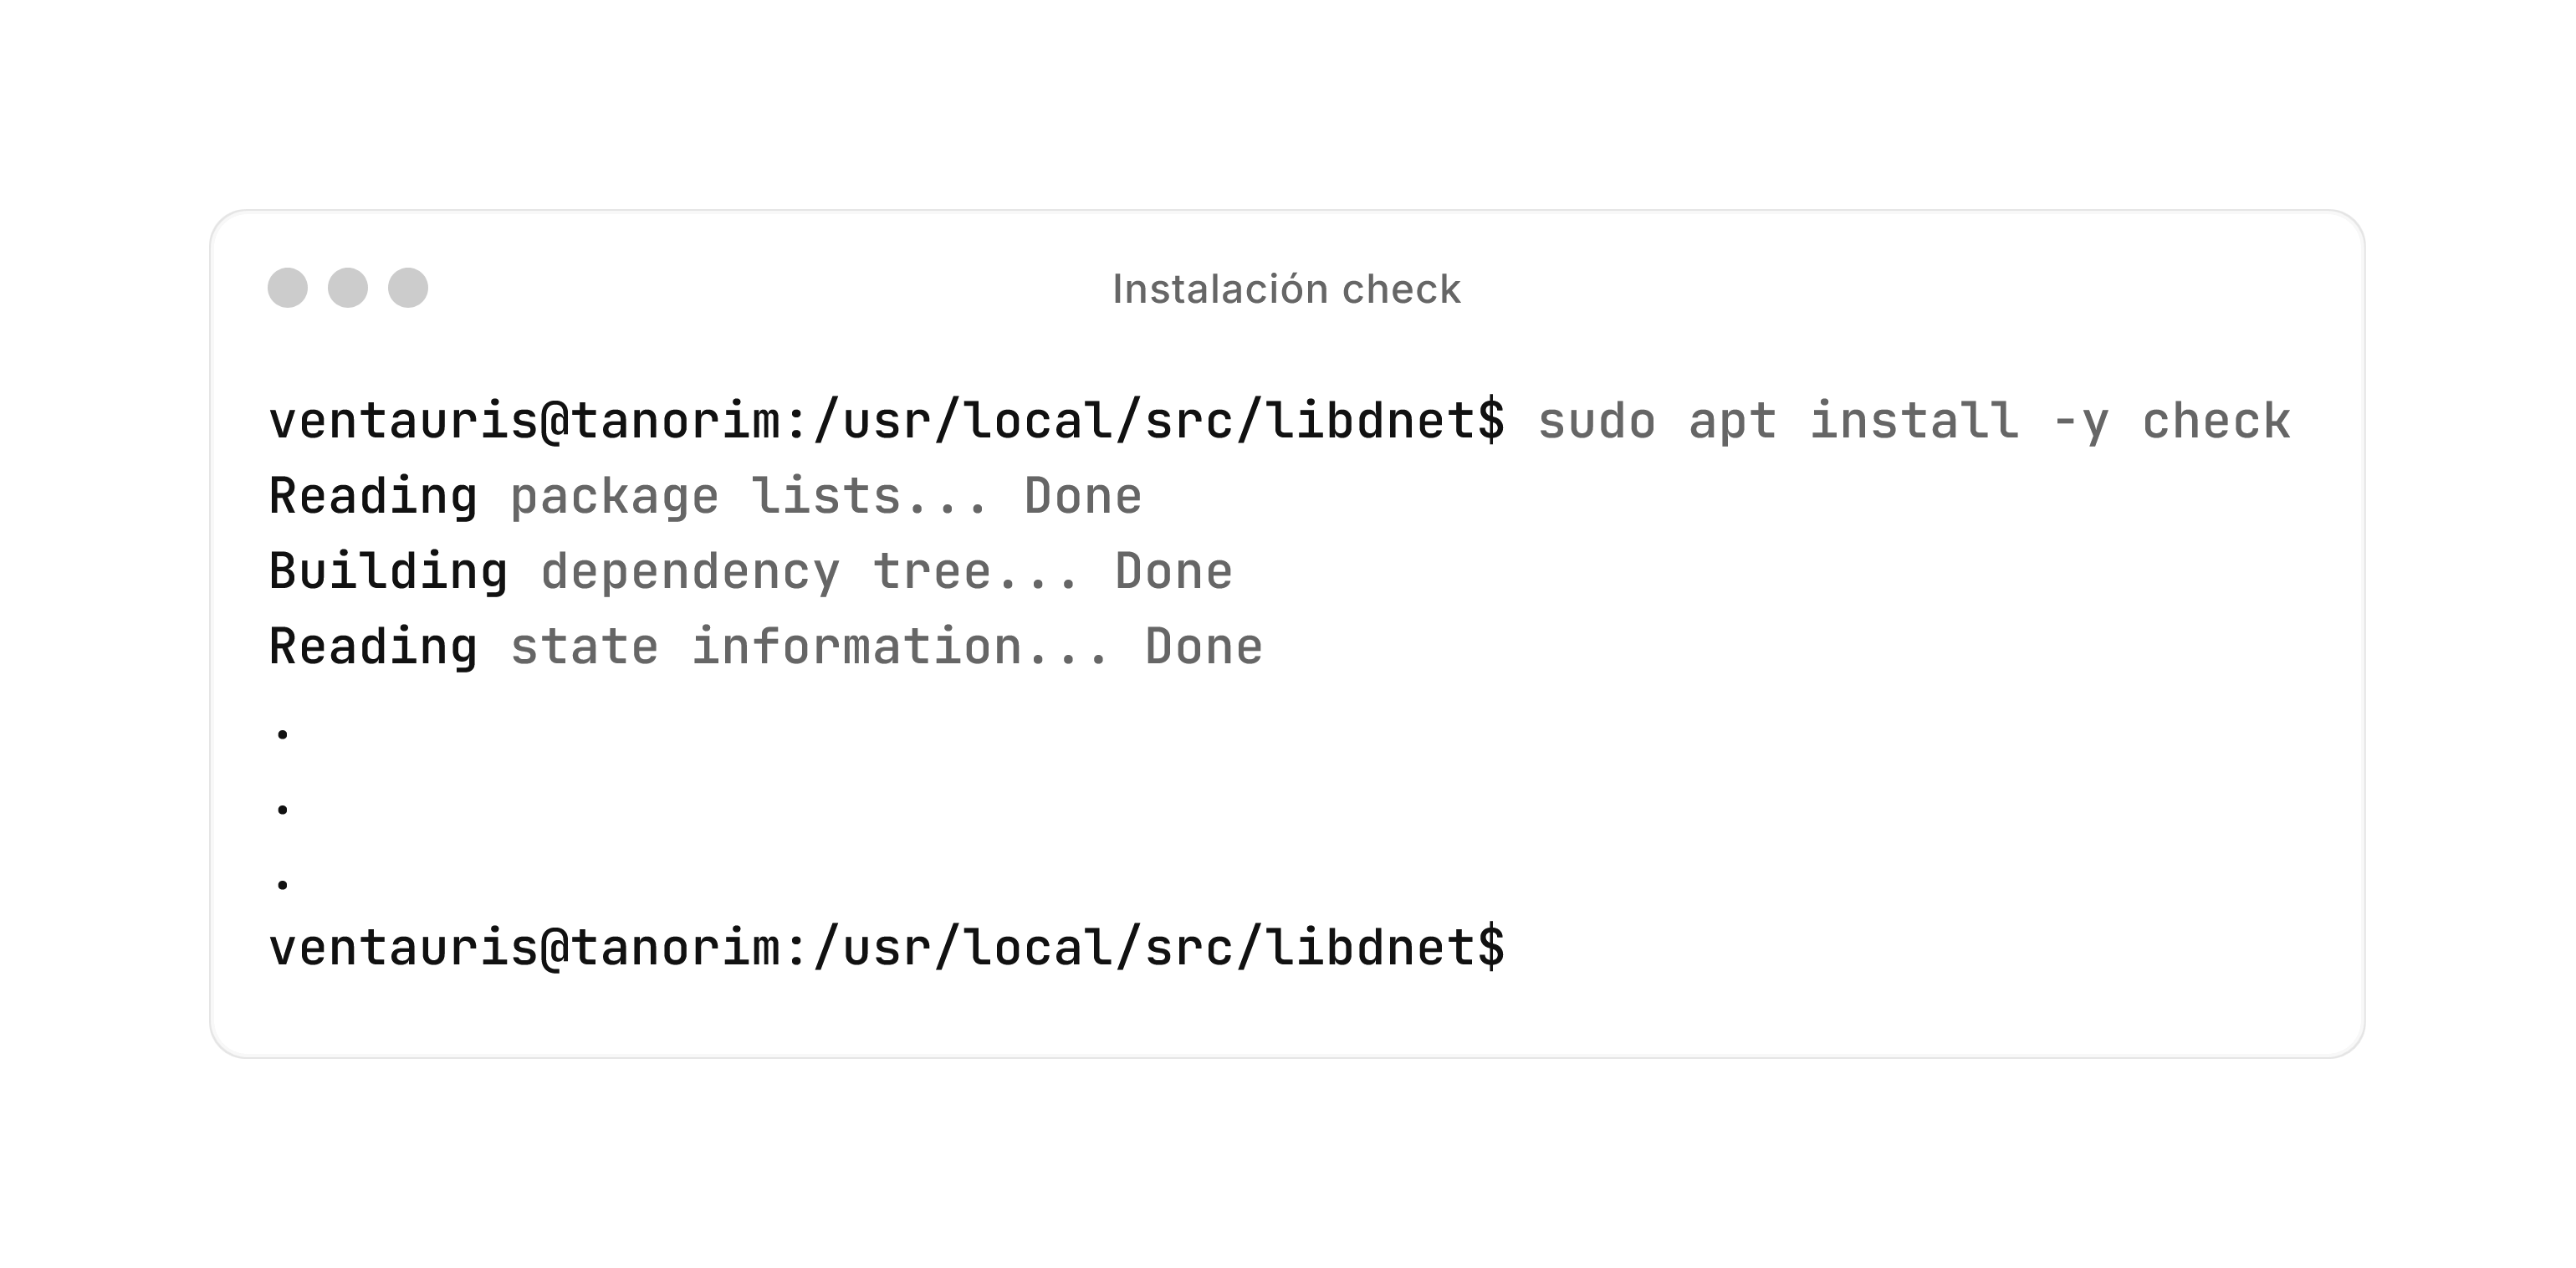
\includegraphics[scale=0.12]{instalacion_snort/2-2.png}
	\caption{Instalando dependencia \texttt{check}.}
\end{figure}

La ejecución de \texttt{./configure} prepara el entorno para la compilación de \texttt{libdnet}, dependencia fundamental para el correcto funcionamiento del desarrollo posterior y de Snort. Su funcionamiento consiste en la revisión del sistema, verifica dependencias y configura los archivos necesarios para compilar código correctamente.

\begin{figure}[H]
	\centering
	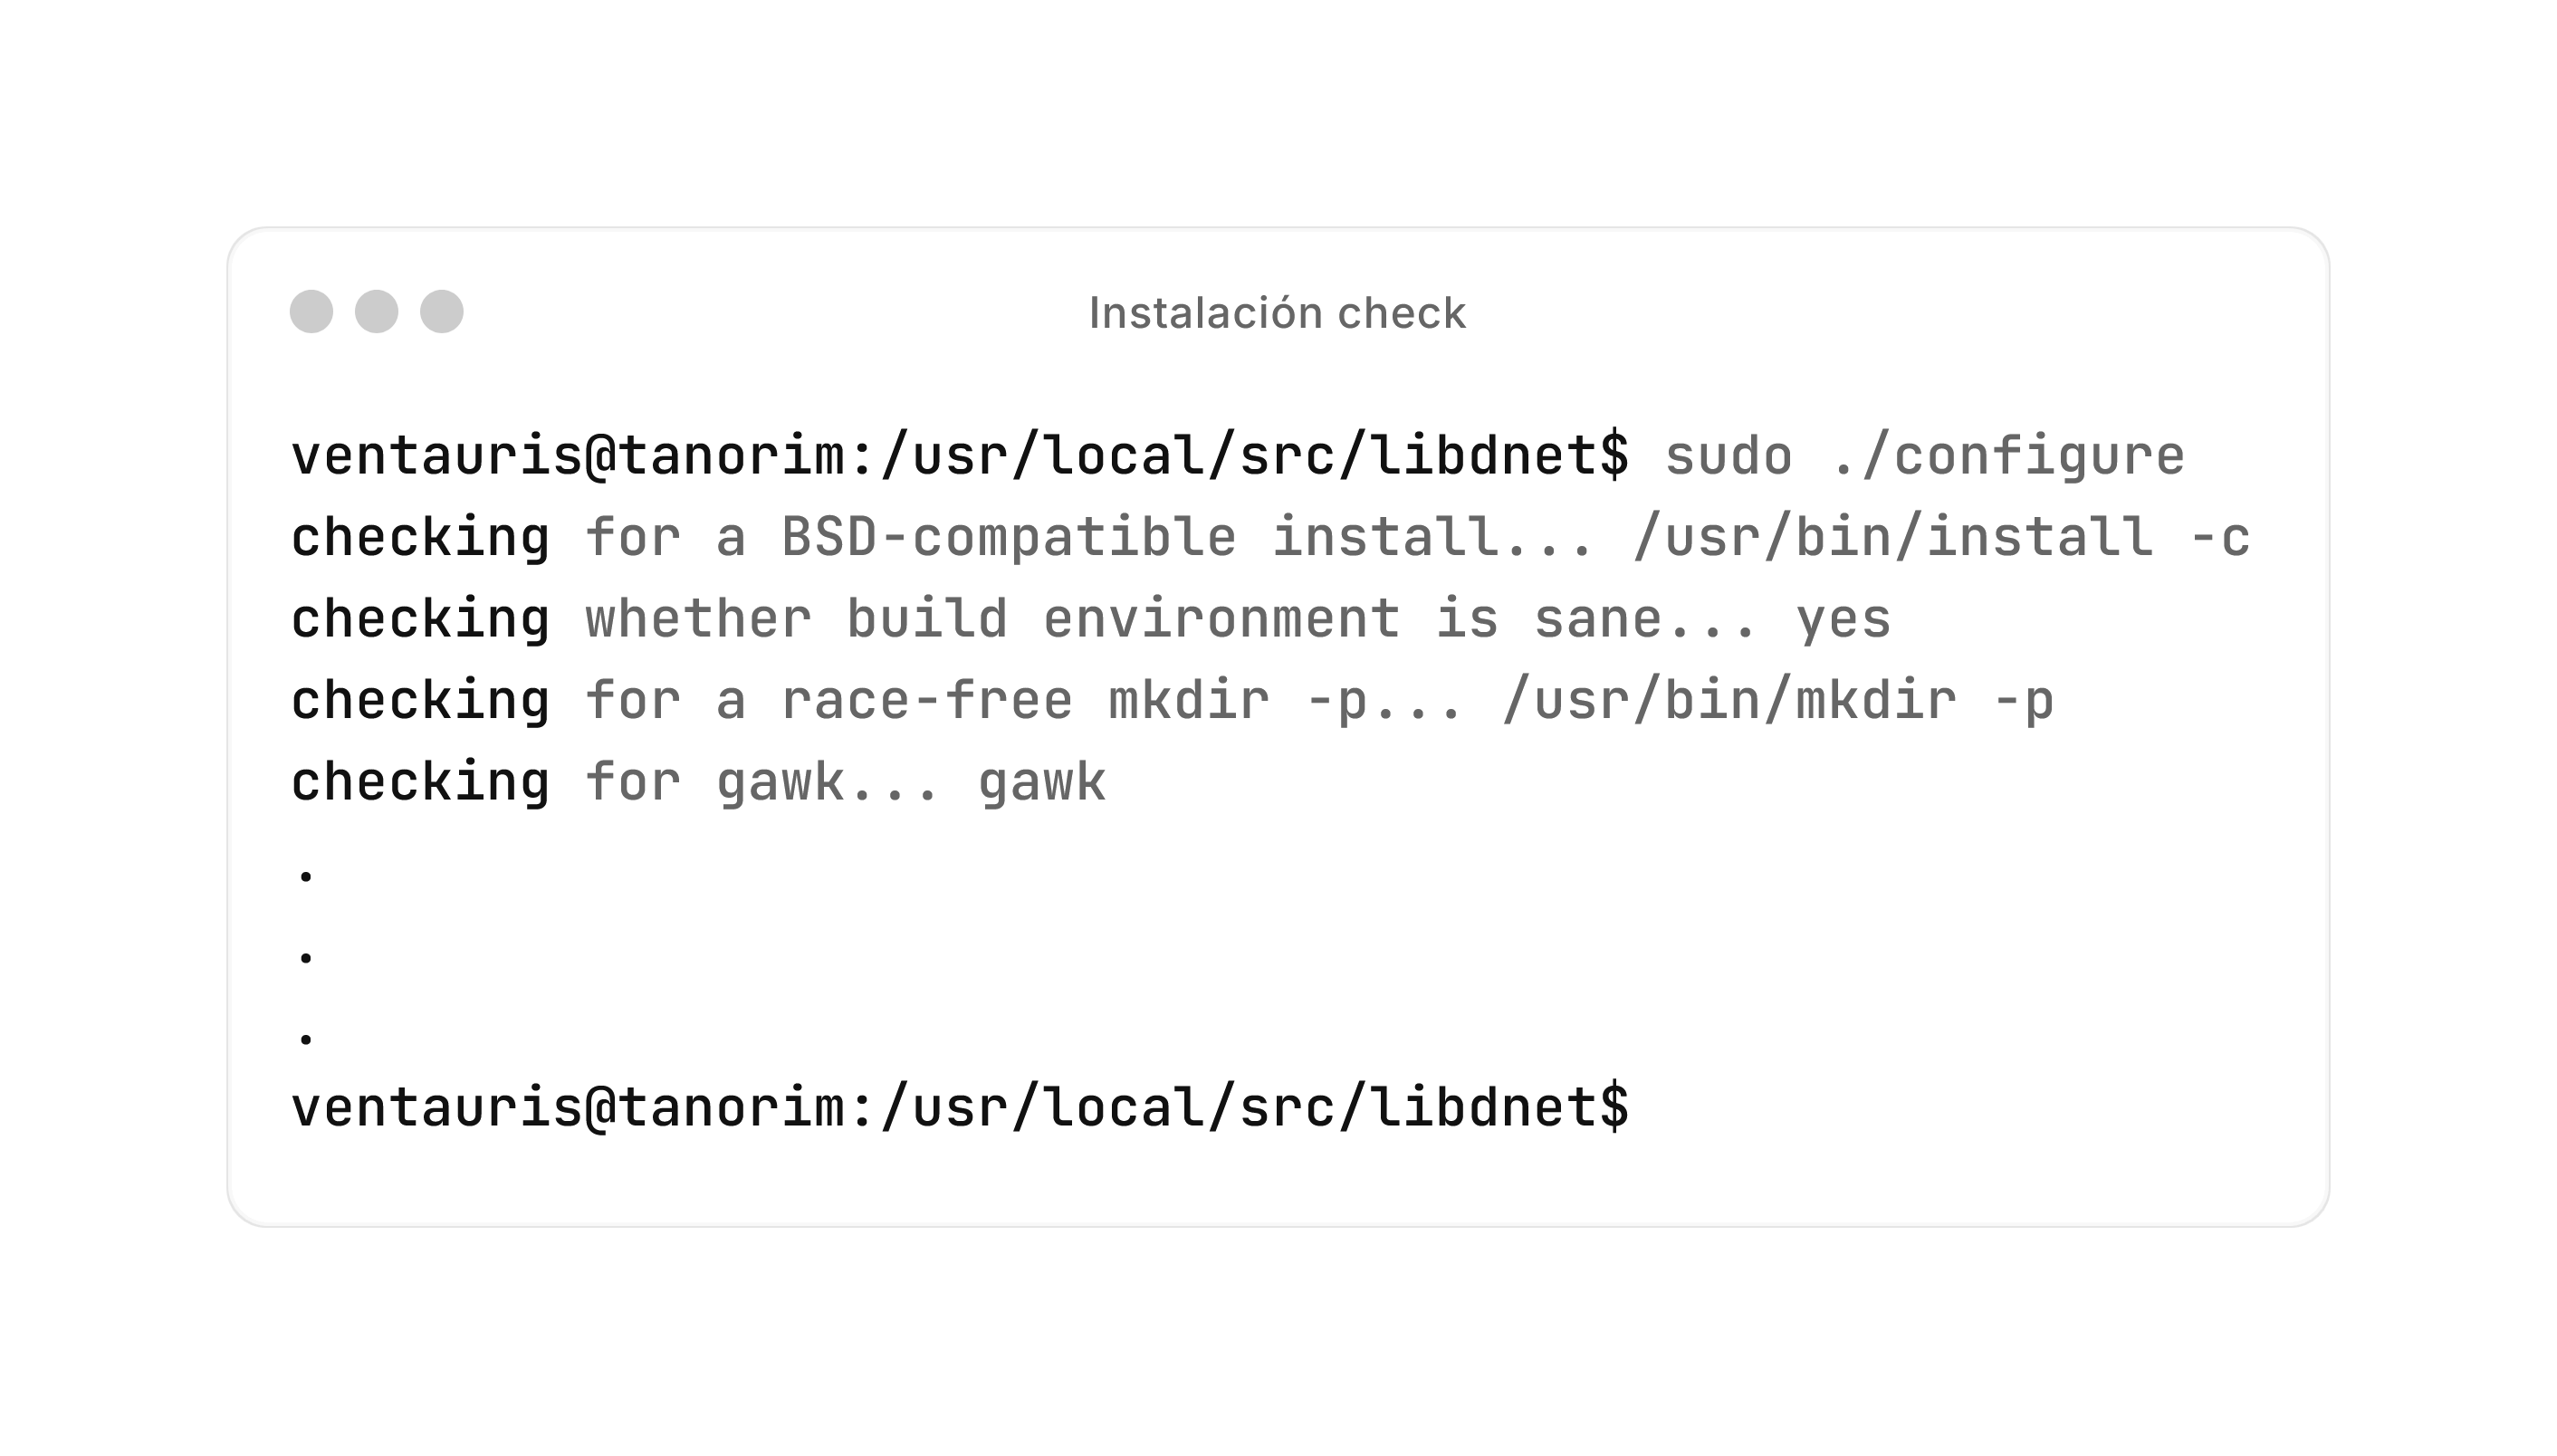
\includegraphics[scale=0.12]{instalacion_snort/3-3.png}
	\caption{Configurando \texttt{libdnet} antes de la compilación.}
\end{figure}

\newpage

Llevamos a cabo la compilación de \texttt{libdnet} mediante \texttt{sudo make}; este comando convierte el código fuente de la dependencia en un ejecutable con bibliotecas a disposición para la instalación. Recorre los directorios del proyecto asegurándose de que todos los archivos necesarios sean procesados.

\begin{figure}[H]
	\centering
	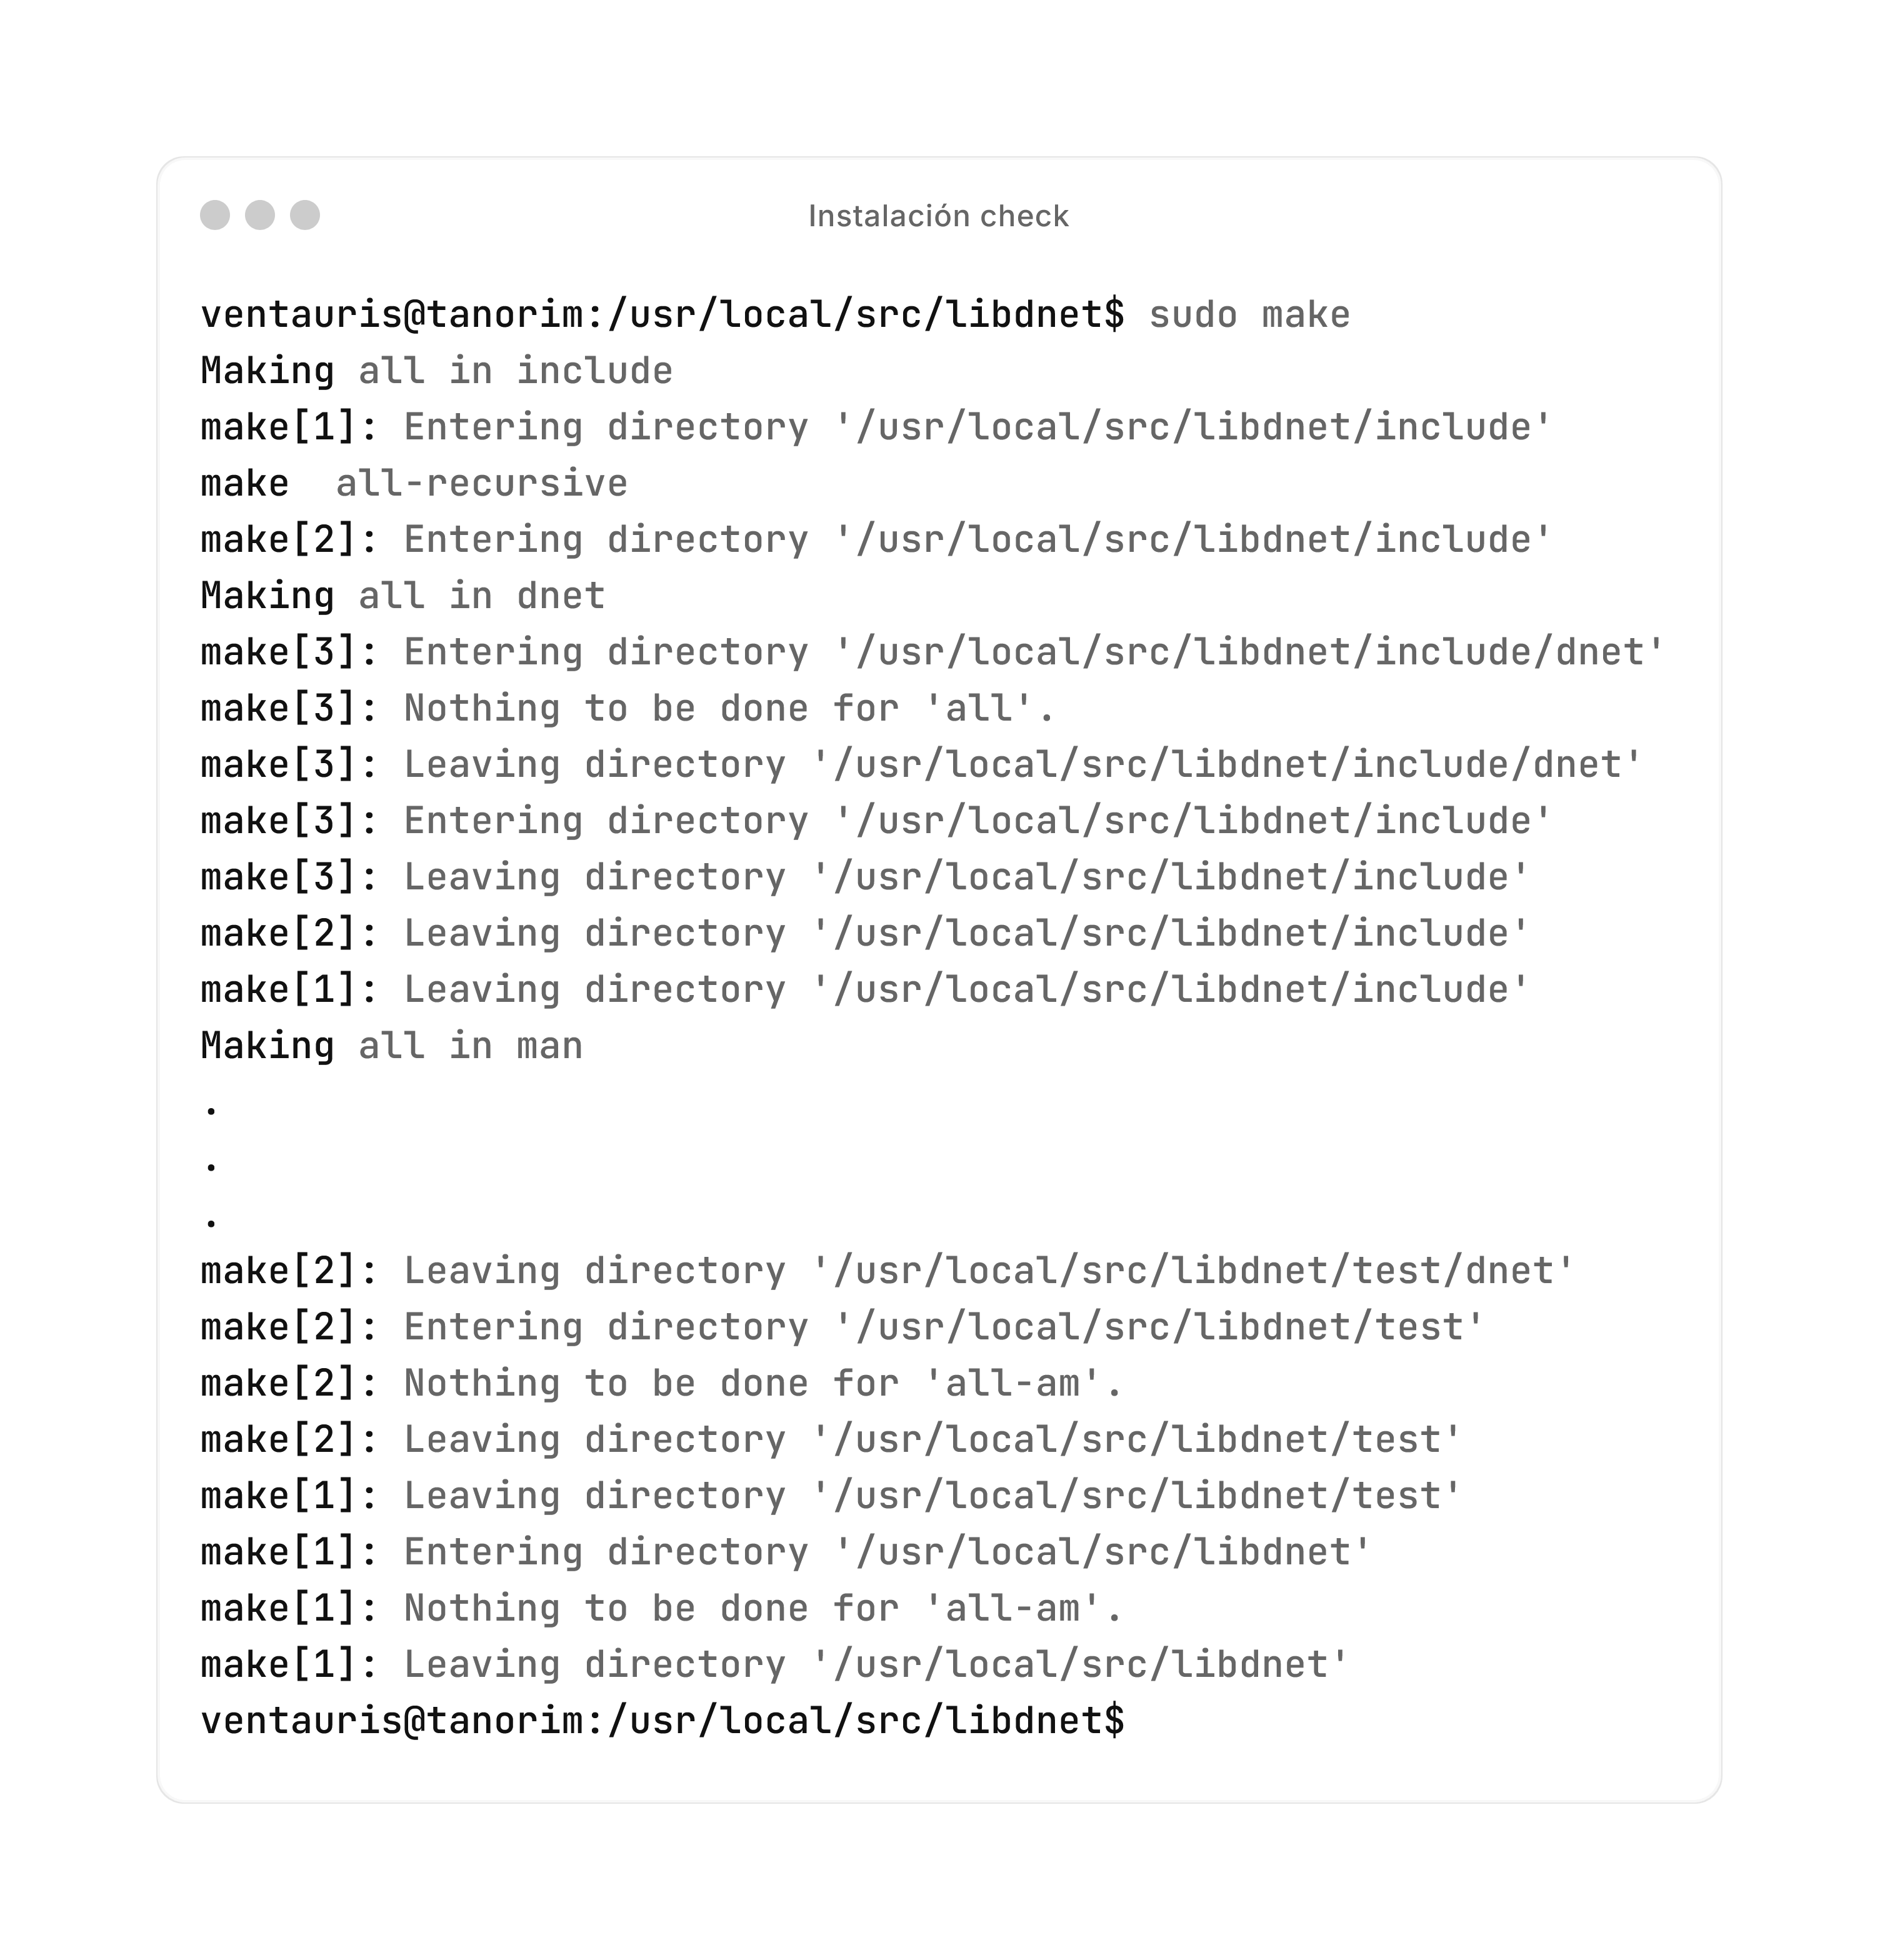
\includegraphics[scale=0.12]{instalacion_snort/4-4.png}
	\caption{Compilando \texttt{libdnet} con \texttt{make}.}
\end{figure}


\newpage

Ahora ejecutamos \texttt{sudo make install} para instalar \texttt{libdnet} en el sistema. Este comando copia los archivos compilados a sus directorios correspondientes, asegurando que puedan ser utilizados por otras aplicaciones y librerías.

\begin{figure}[H]
	\centering
	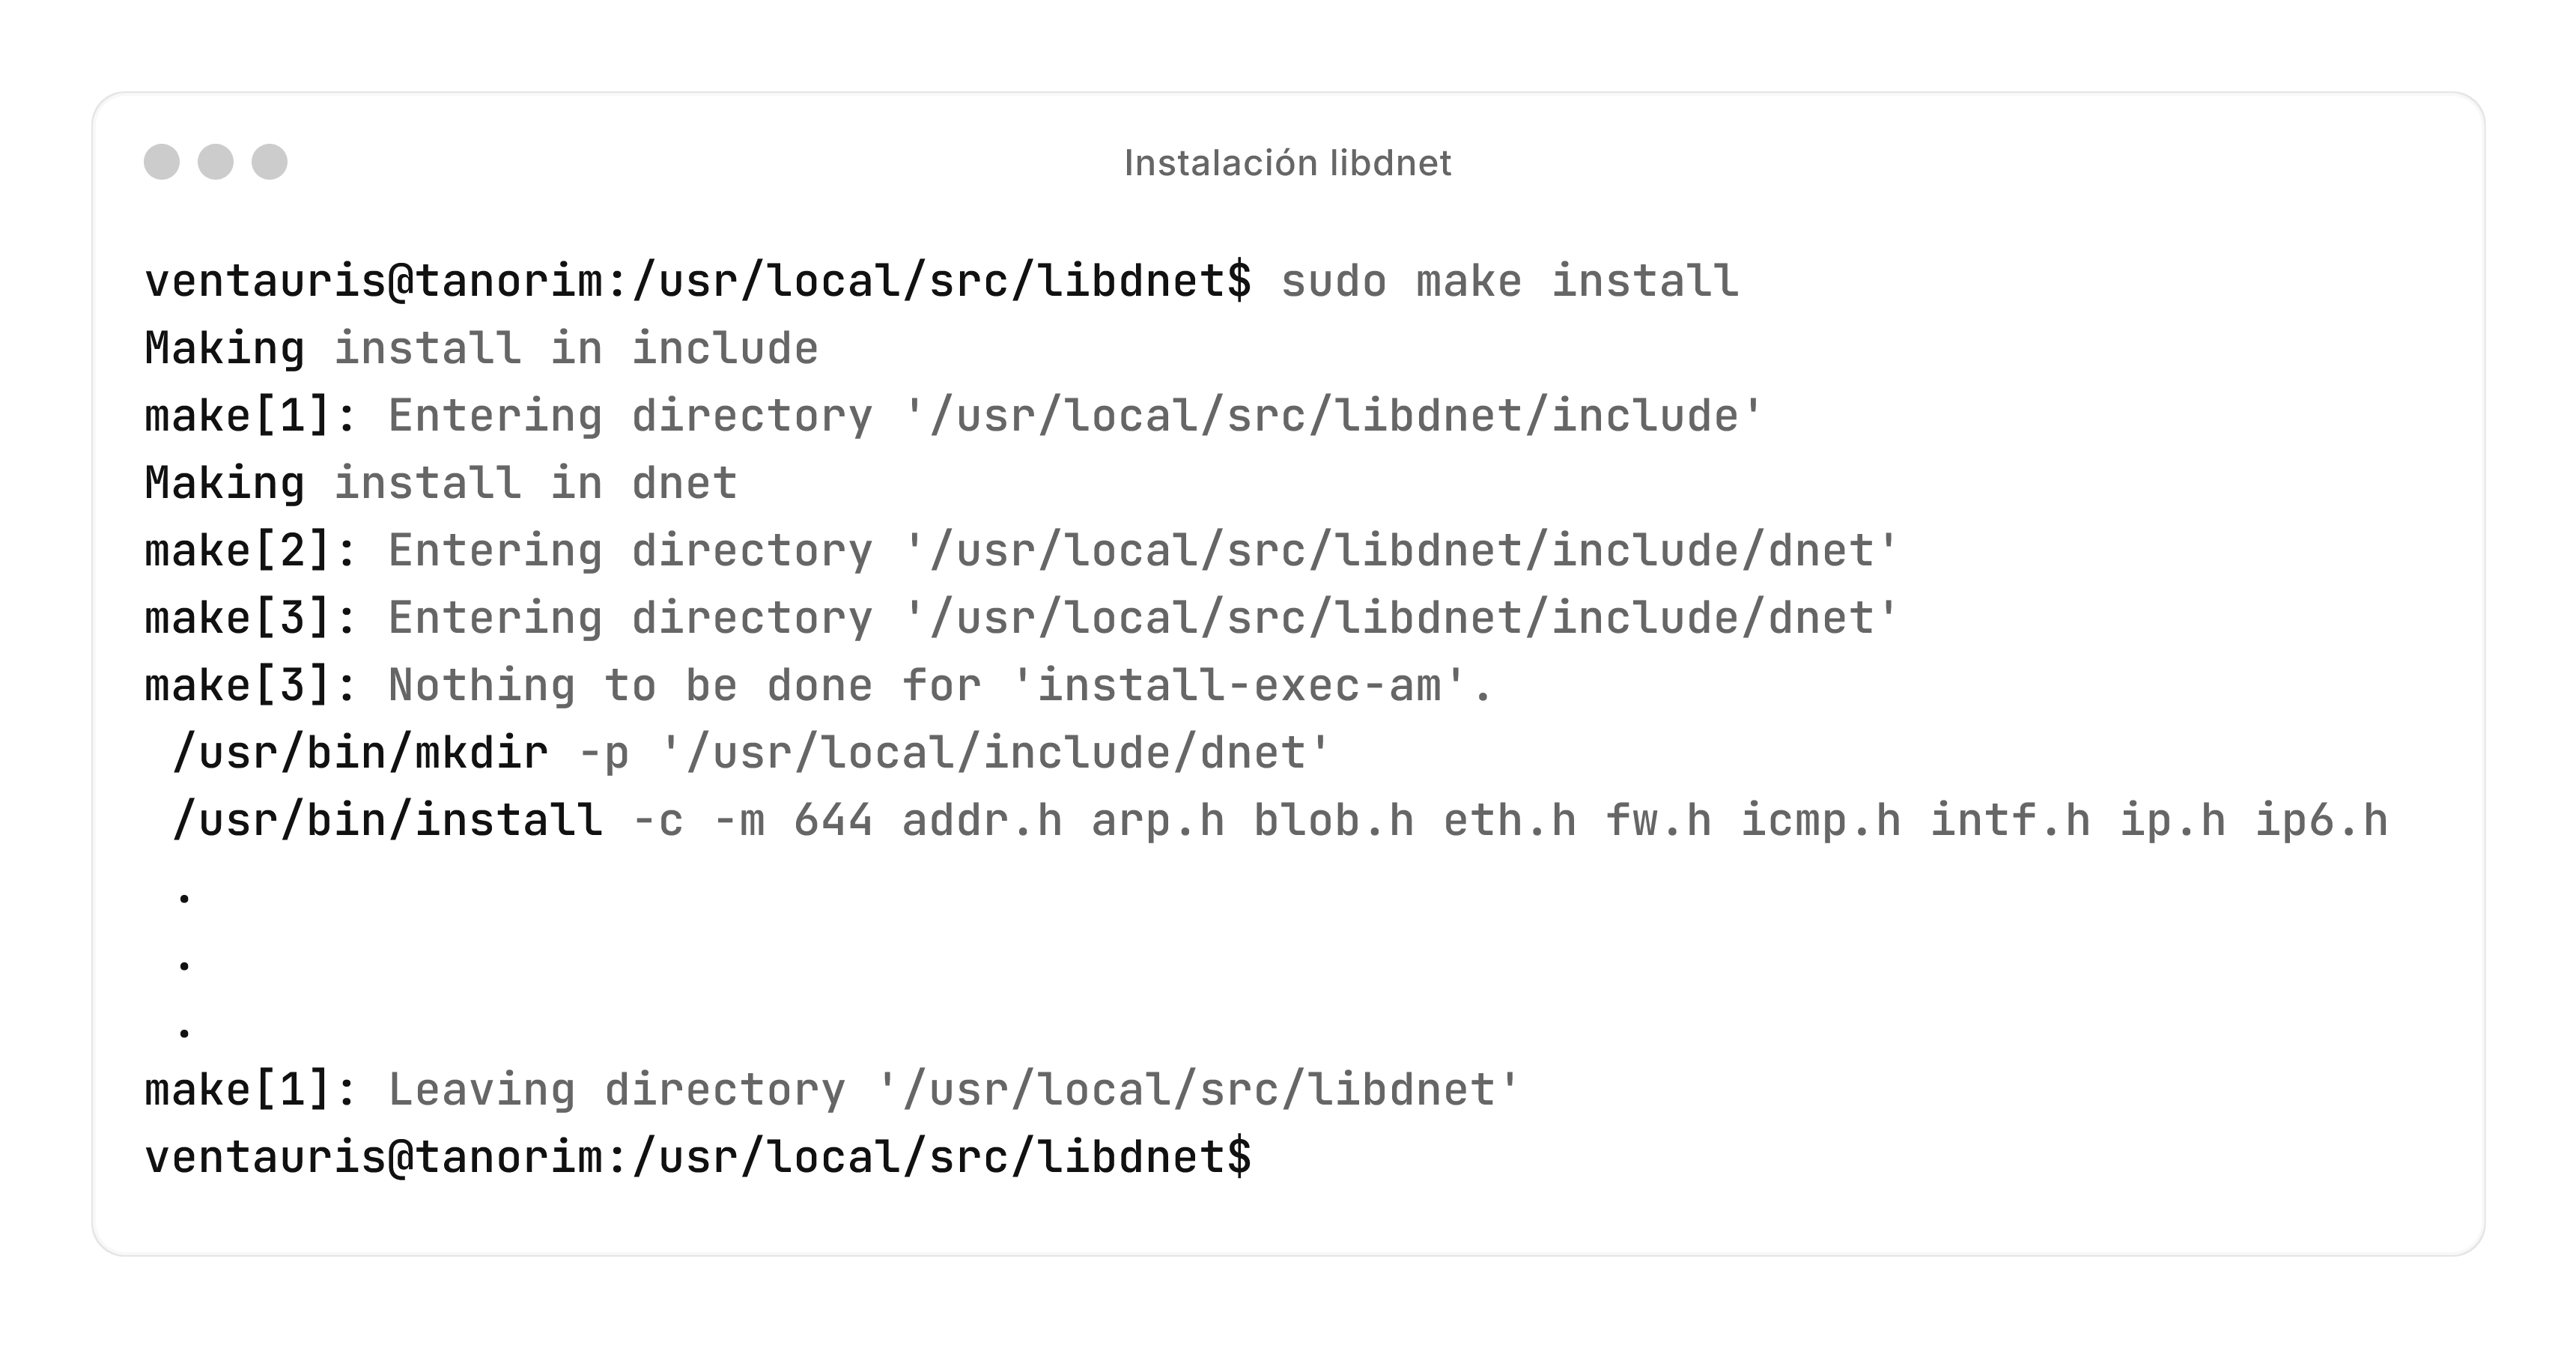
\includegraphics[scale=0.12]{instalacion_snort/5-5.png}
	\caption{Instalando \texttt{libdnet} en el sistema.}
\end{figure}

\subsubsection*{Solución al problema de \texttt{PKG\_CONFIG\_PATH}}

Listamos los archivos de \texttt{libdnet} en \texttt{/usr/local/lib} para asegurarnos de que se instalaron correctamente. Luego, intentamos verificar su versión con \texttt{pkg-config --modversion dnet}, pero aparece un error indicando que no se encuentra en el \texttt{PKG\_CONFIG\_PATH}. Esto indica que es necesario añadir la ruta correcta para que el sistema reconozca la librería.

\begin{figure}[H]
	\centering
	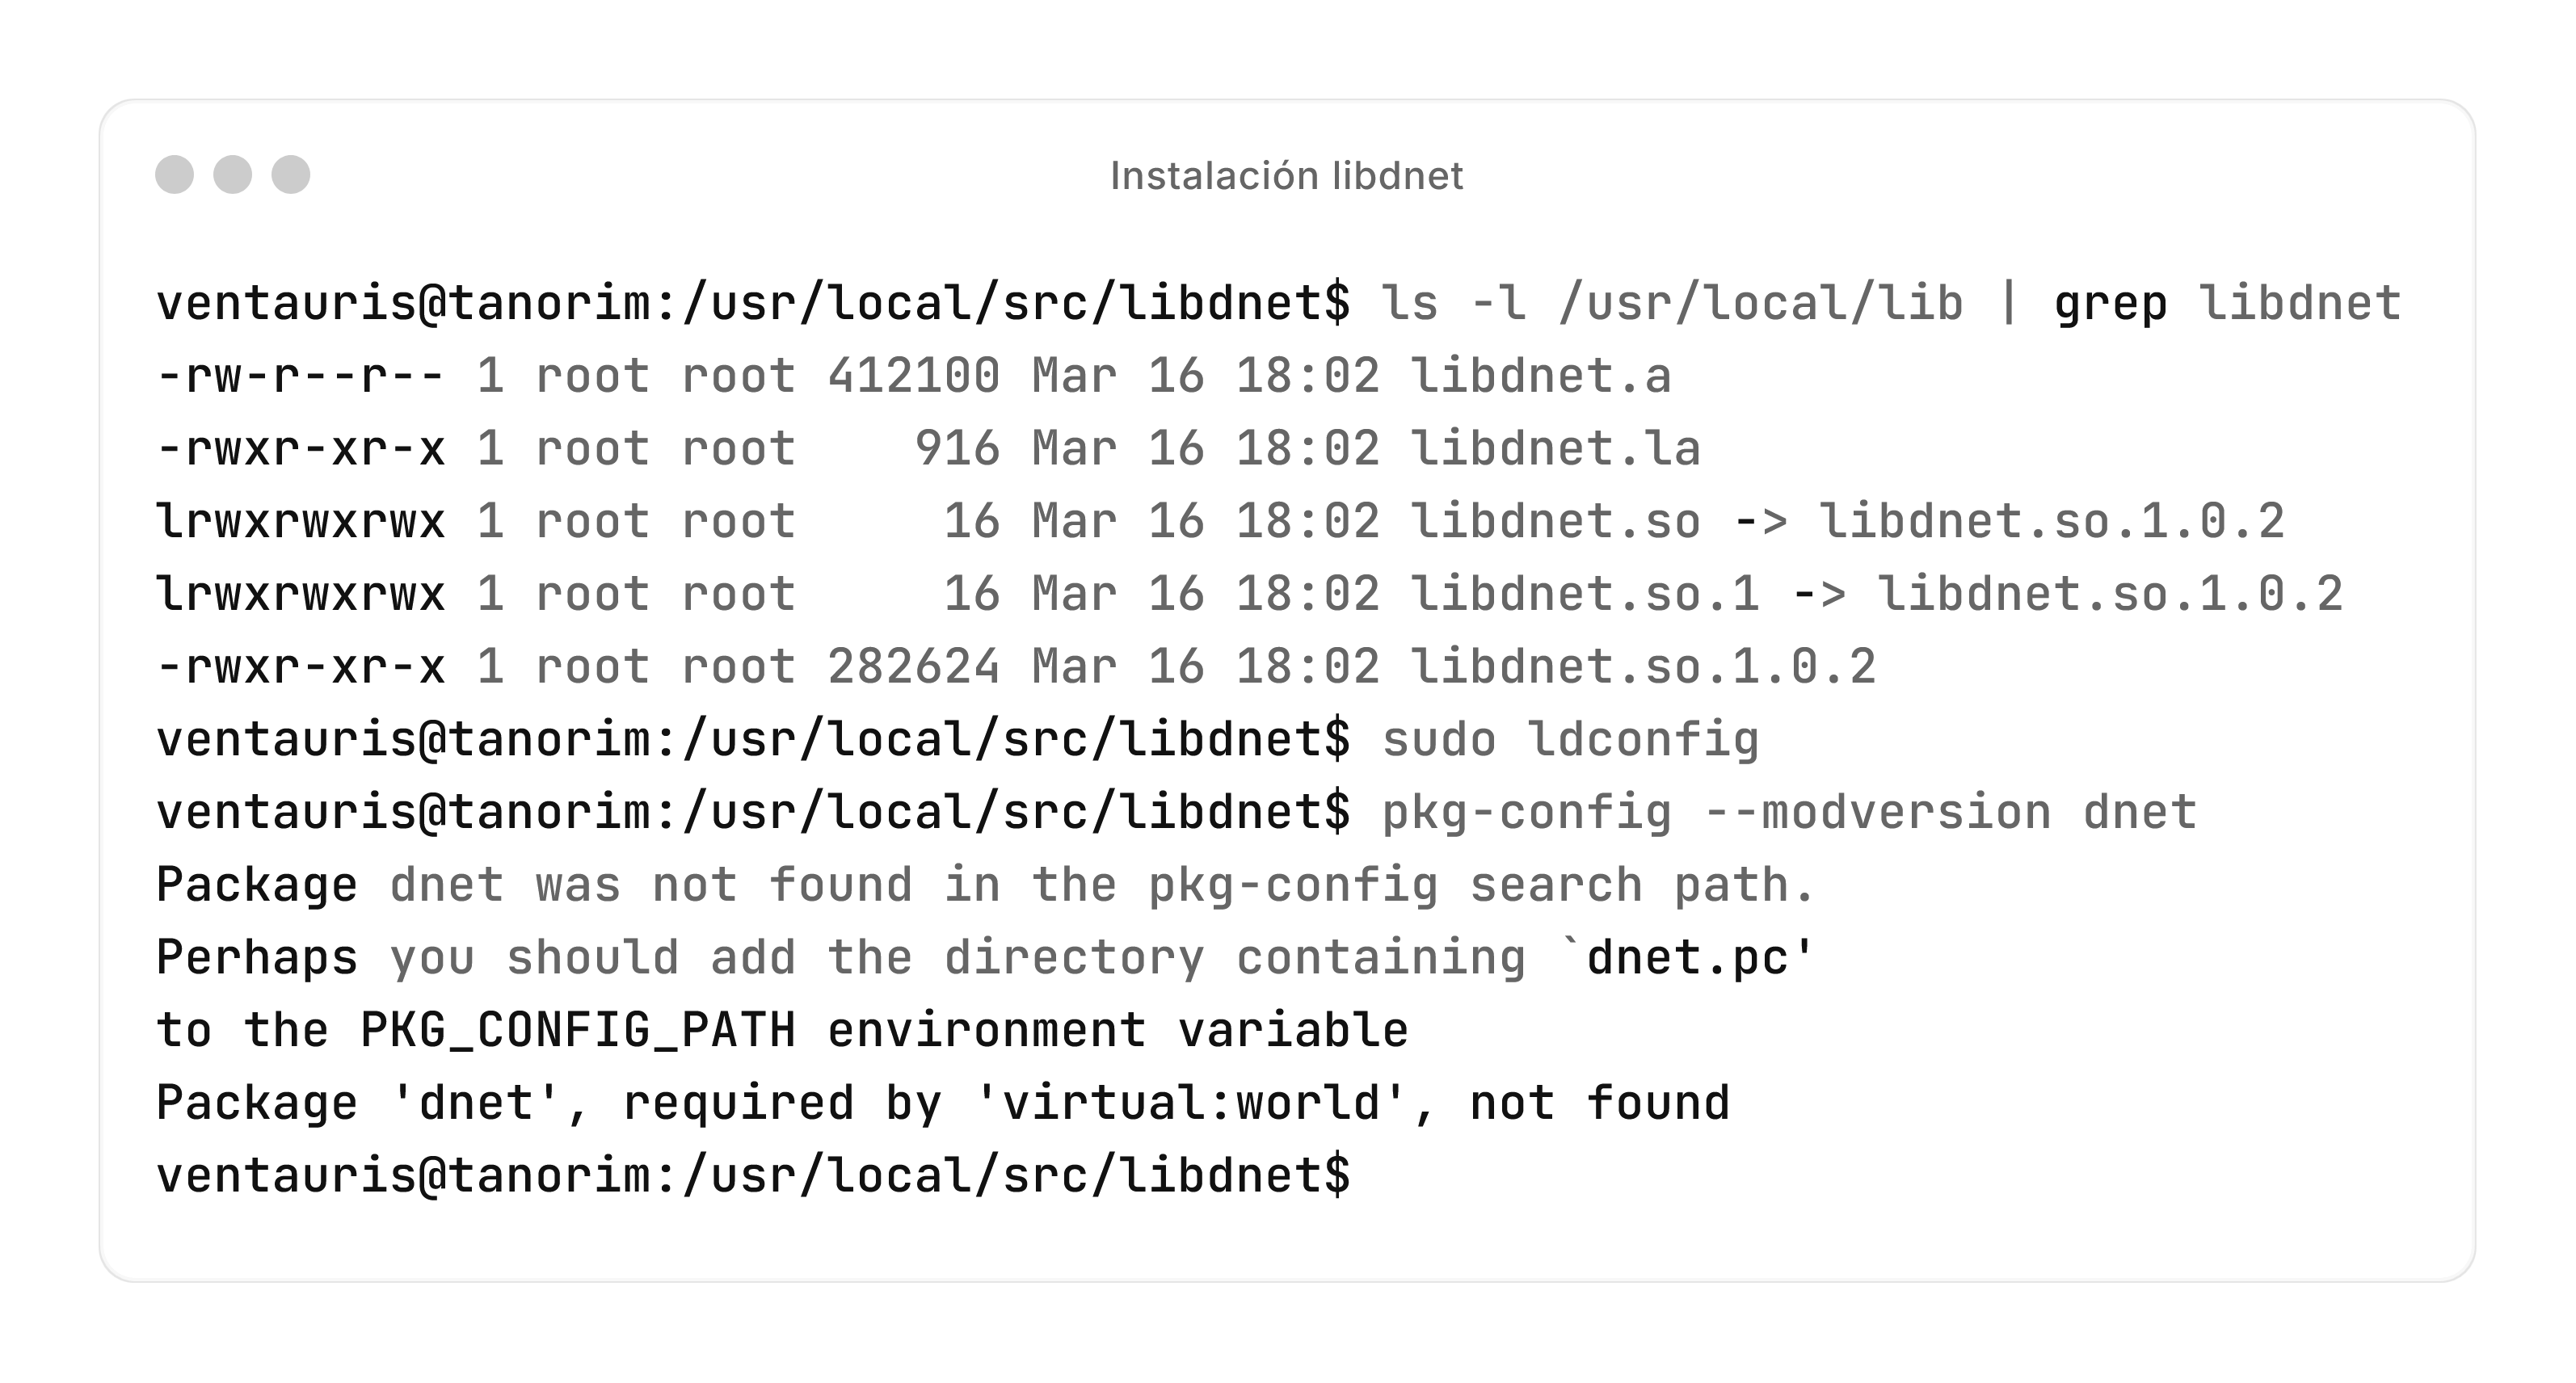
\includegraphics[scale=0.12]{instalacion_snort/6-6.png}
	\caption{Verificación de la instalación de \texttt{libdnet}.}
\end{figure}

\newpage

Editamos el archivo \texttt{dnet.pc} usando \texttt{nano}, añadiendo las rutas correctas para que \texttt{pkg-config} pueda encontrar \texttt{libdnet}. Definimos las variables \texttt{libdir} e \texttt{includedir}, asegurándonos de que apunten a \texttt{/usr/local/lib} y \texttt{/usr/local/include}, respectivamente. Esto soluciona el problema anterior donde \texttt{pkg-config} no encontraba la librería.

\begin{figure}[H]
	\centering
	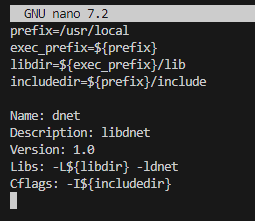
\includegraphics[scale=1]{instalacion_snort/7.png}
	\caption{Configurando \texttt{libdnet} para que sea reconocido por el sistema.}
\end{figure}

Ahora configuramos el entorno para que \texttt{pkg-config} pueda encontrar \texttt{libdnet}. Primero, exportamos la variable \texttt{PKG\_CONFIG\_PATH} con la ruta correcta y la agregamos permanentemente al archivo \texttt{\~{}/.bashrc}. Luego, recargamos la configuración con \texttt{source ~/.bashrc}, actualizamos las librerías con \texttt{ldconfig} y verificamos que \texttt{libdnet} es reconocido correctamente ejecutando \texttt{pkg-config --modversion dnet}, confirmando la versión instalada.

\begin{figure}[H]
	\centering
	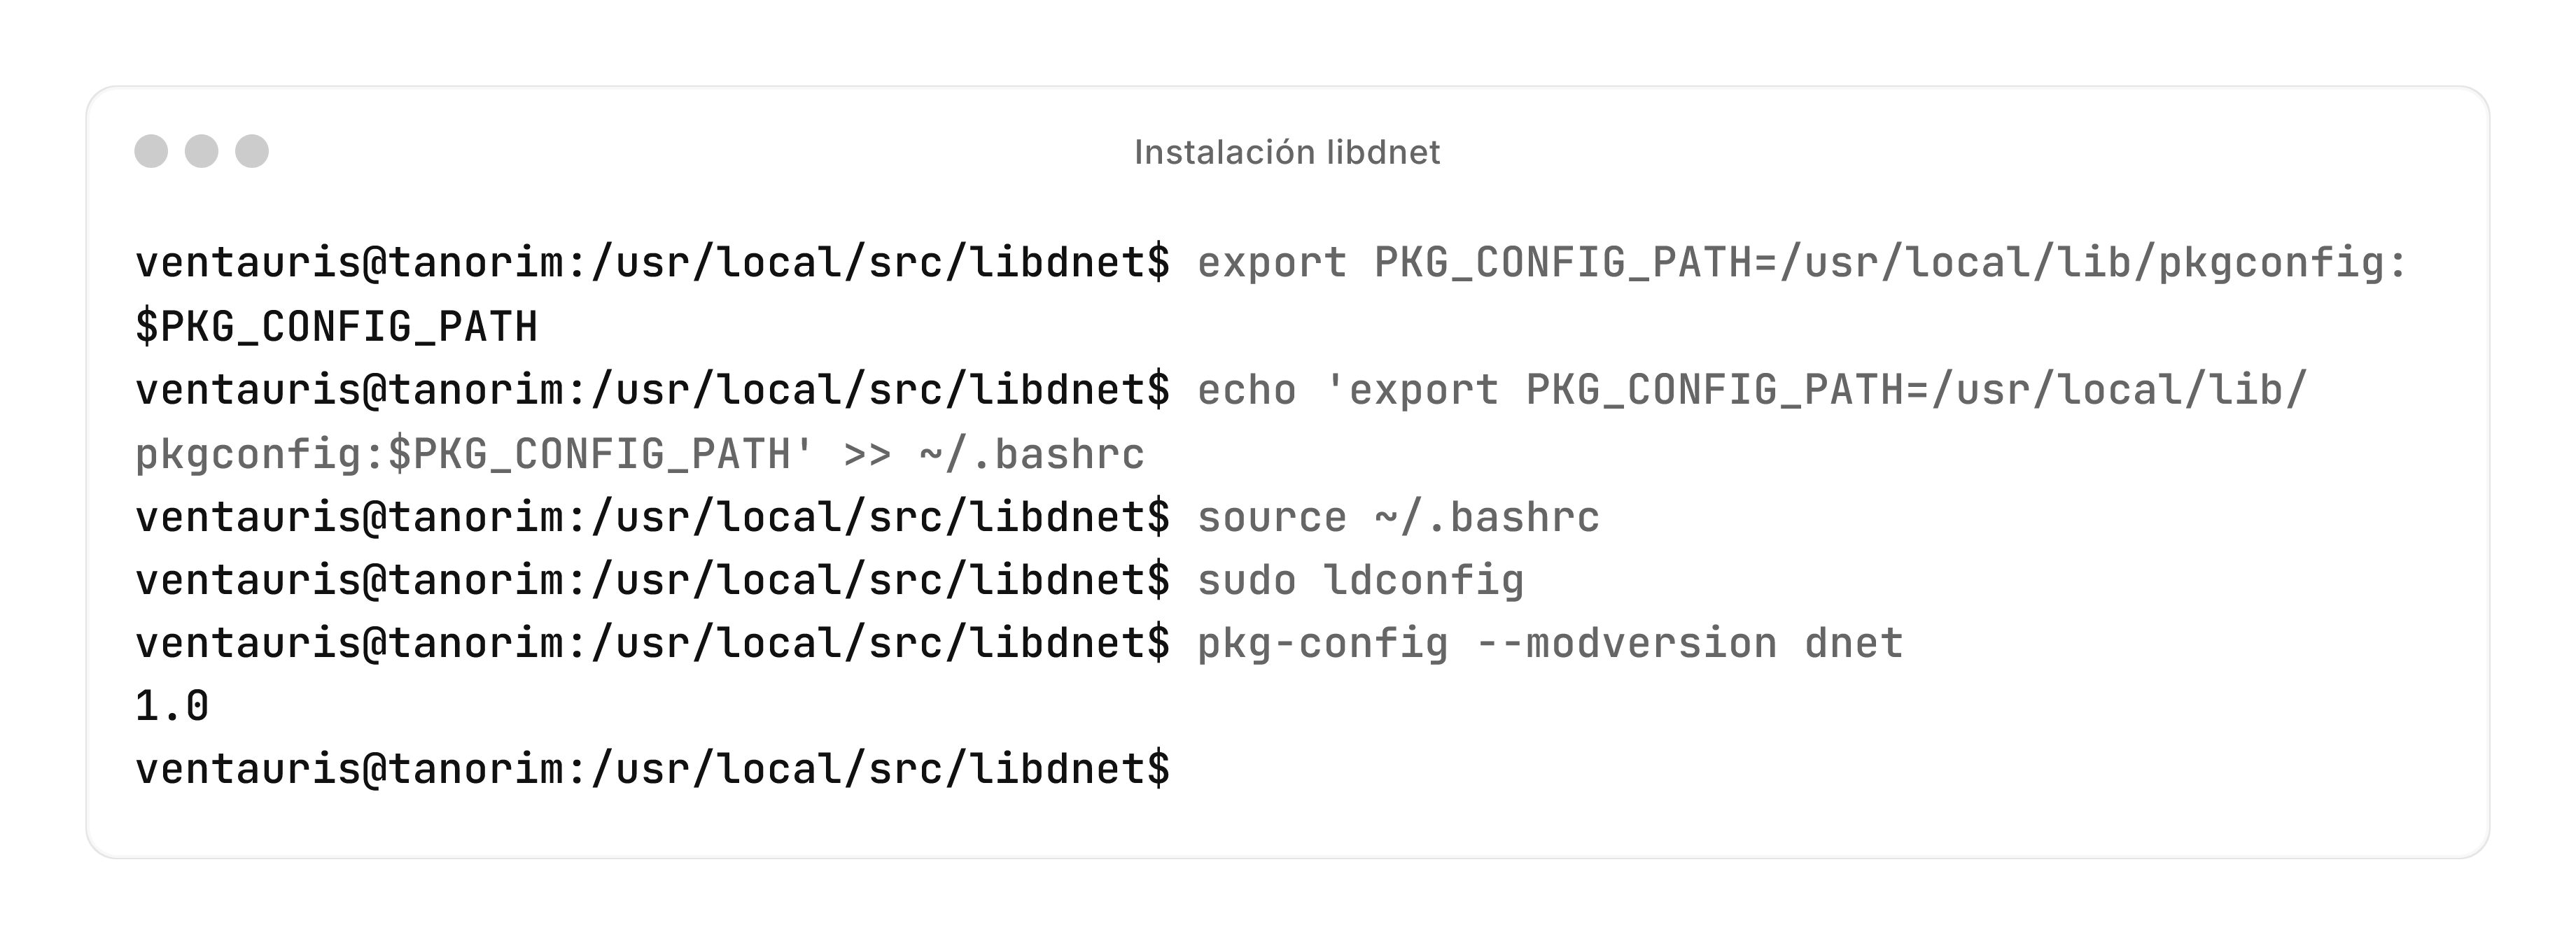
\includegraphics[scale=0.12]{instalacion_snort/8-8.png}
	\caption{Añadiendo \texttt{libdnet} al \texttt{PATH} y verificando su reconocimiento.}
\end{figure}

\newpage

\subsubsection*{Compilación e instalación de \texttt{libdaq}}

Clonamos el repositorio de \texttt{libdaq}, un componente necesario para \textbf{Snort 3}, desde su fuente oficial en GitHub. Este paso descarga el código fuente necesario para su compilación e instalación en la \textbf{Raspberry Pi}.

\begin{figure}[H]
	\centering
	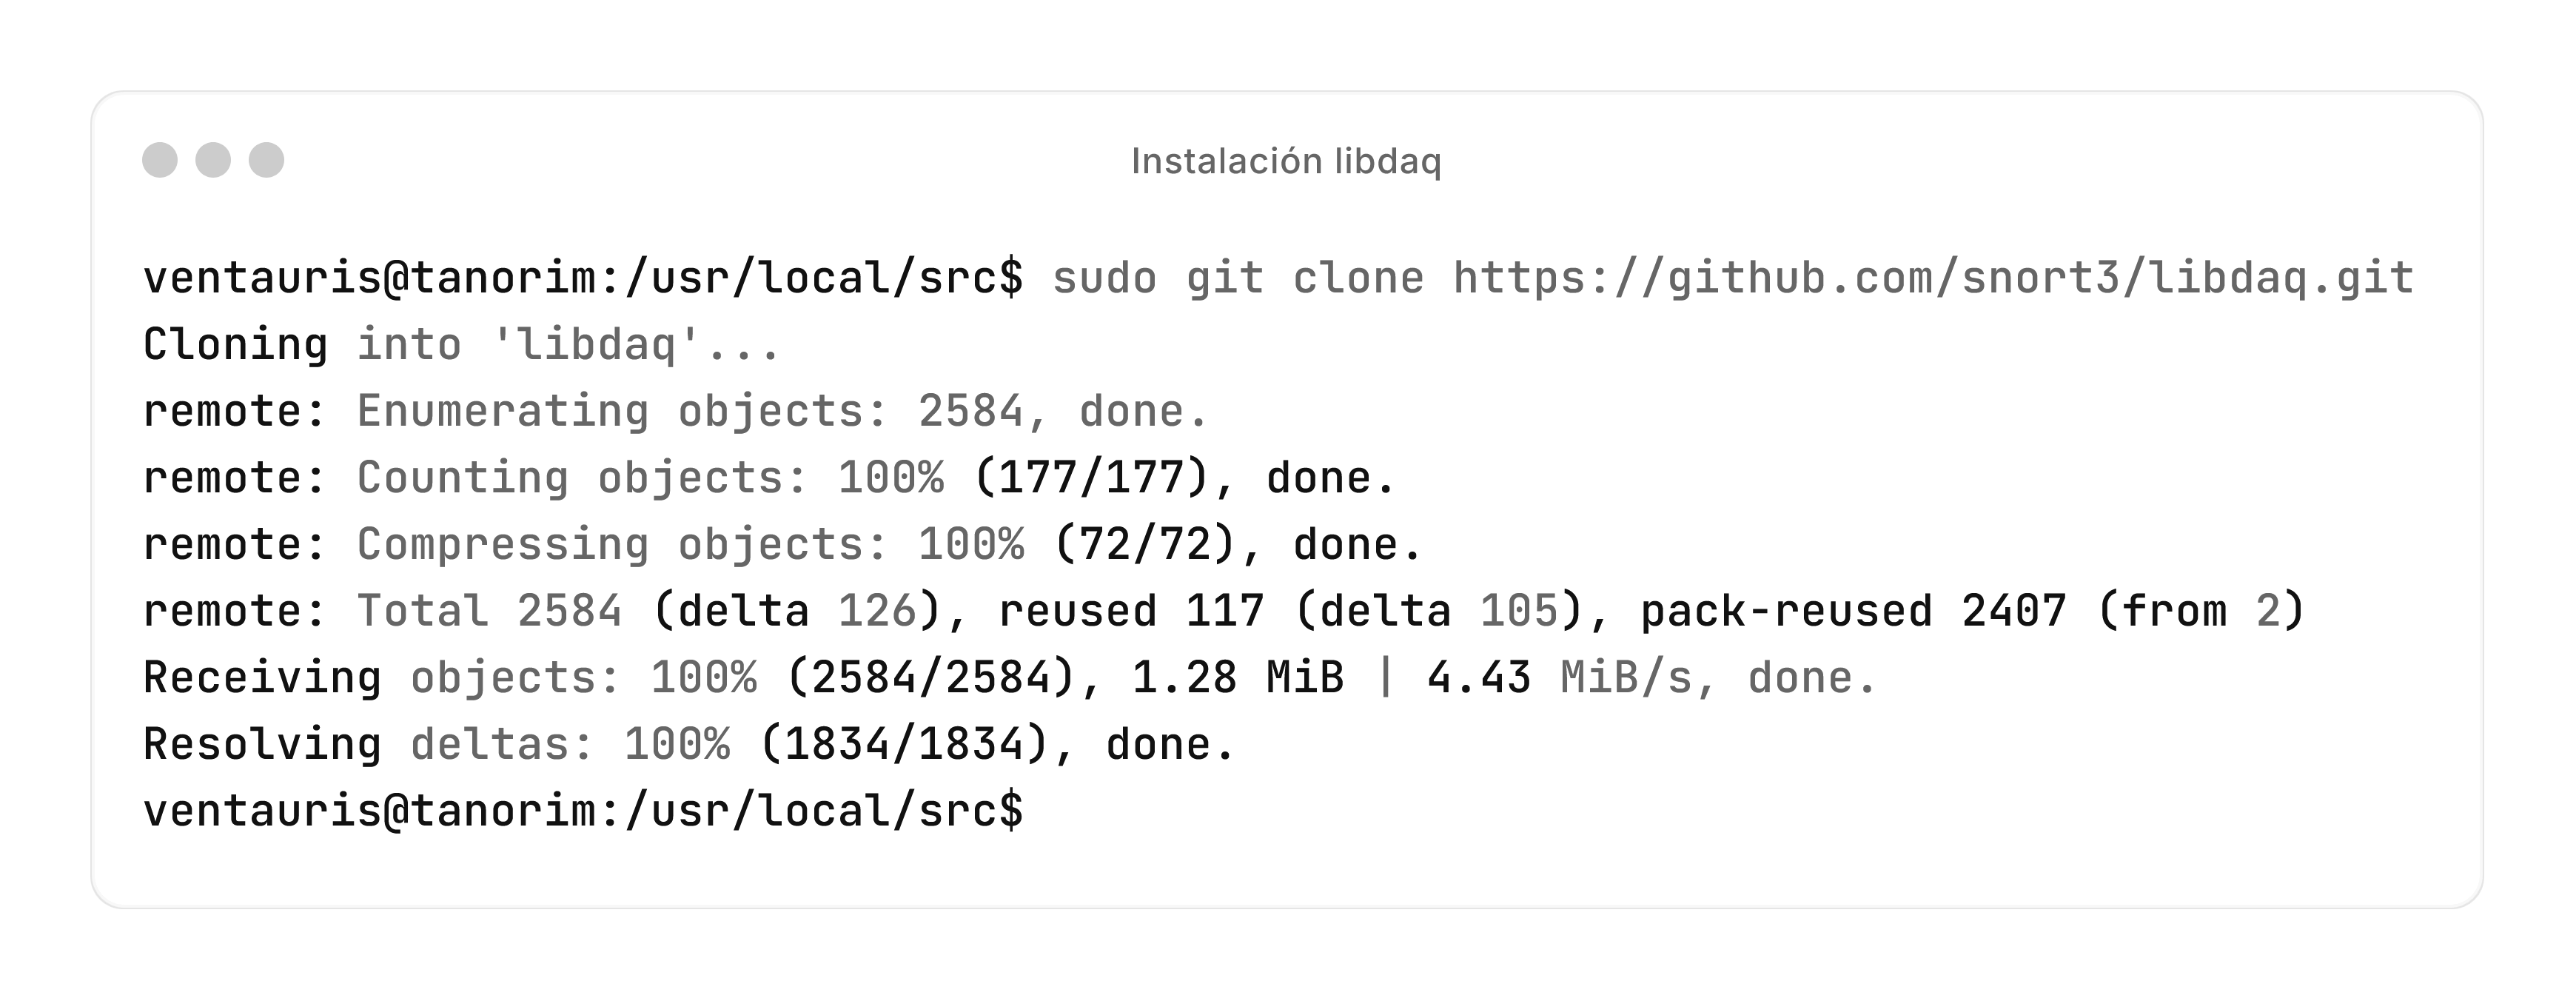
\includegraphics[scale=0.12]{instalacion_snort/9-9.png}
	\caption{Descargando \texttt{libdaq} desde el repositorio oficial.}
\end{figure}

Entramos en el directorio de \texttt{libdaq} y ejecutamos el script \texttt{bootstrap}, que se encarga de generar los archivos de configuración necesarios para compilar el software correctamente. Se usa \texttt{autoreconf} para asegurarse de que todos los scripts de compilación estén en orden.

\begin{figure}[H]
	\centering
	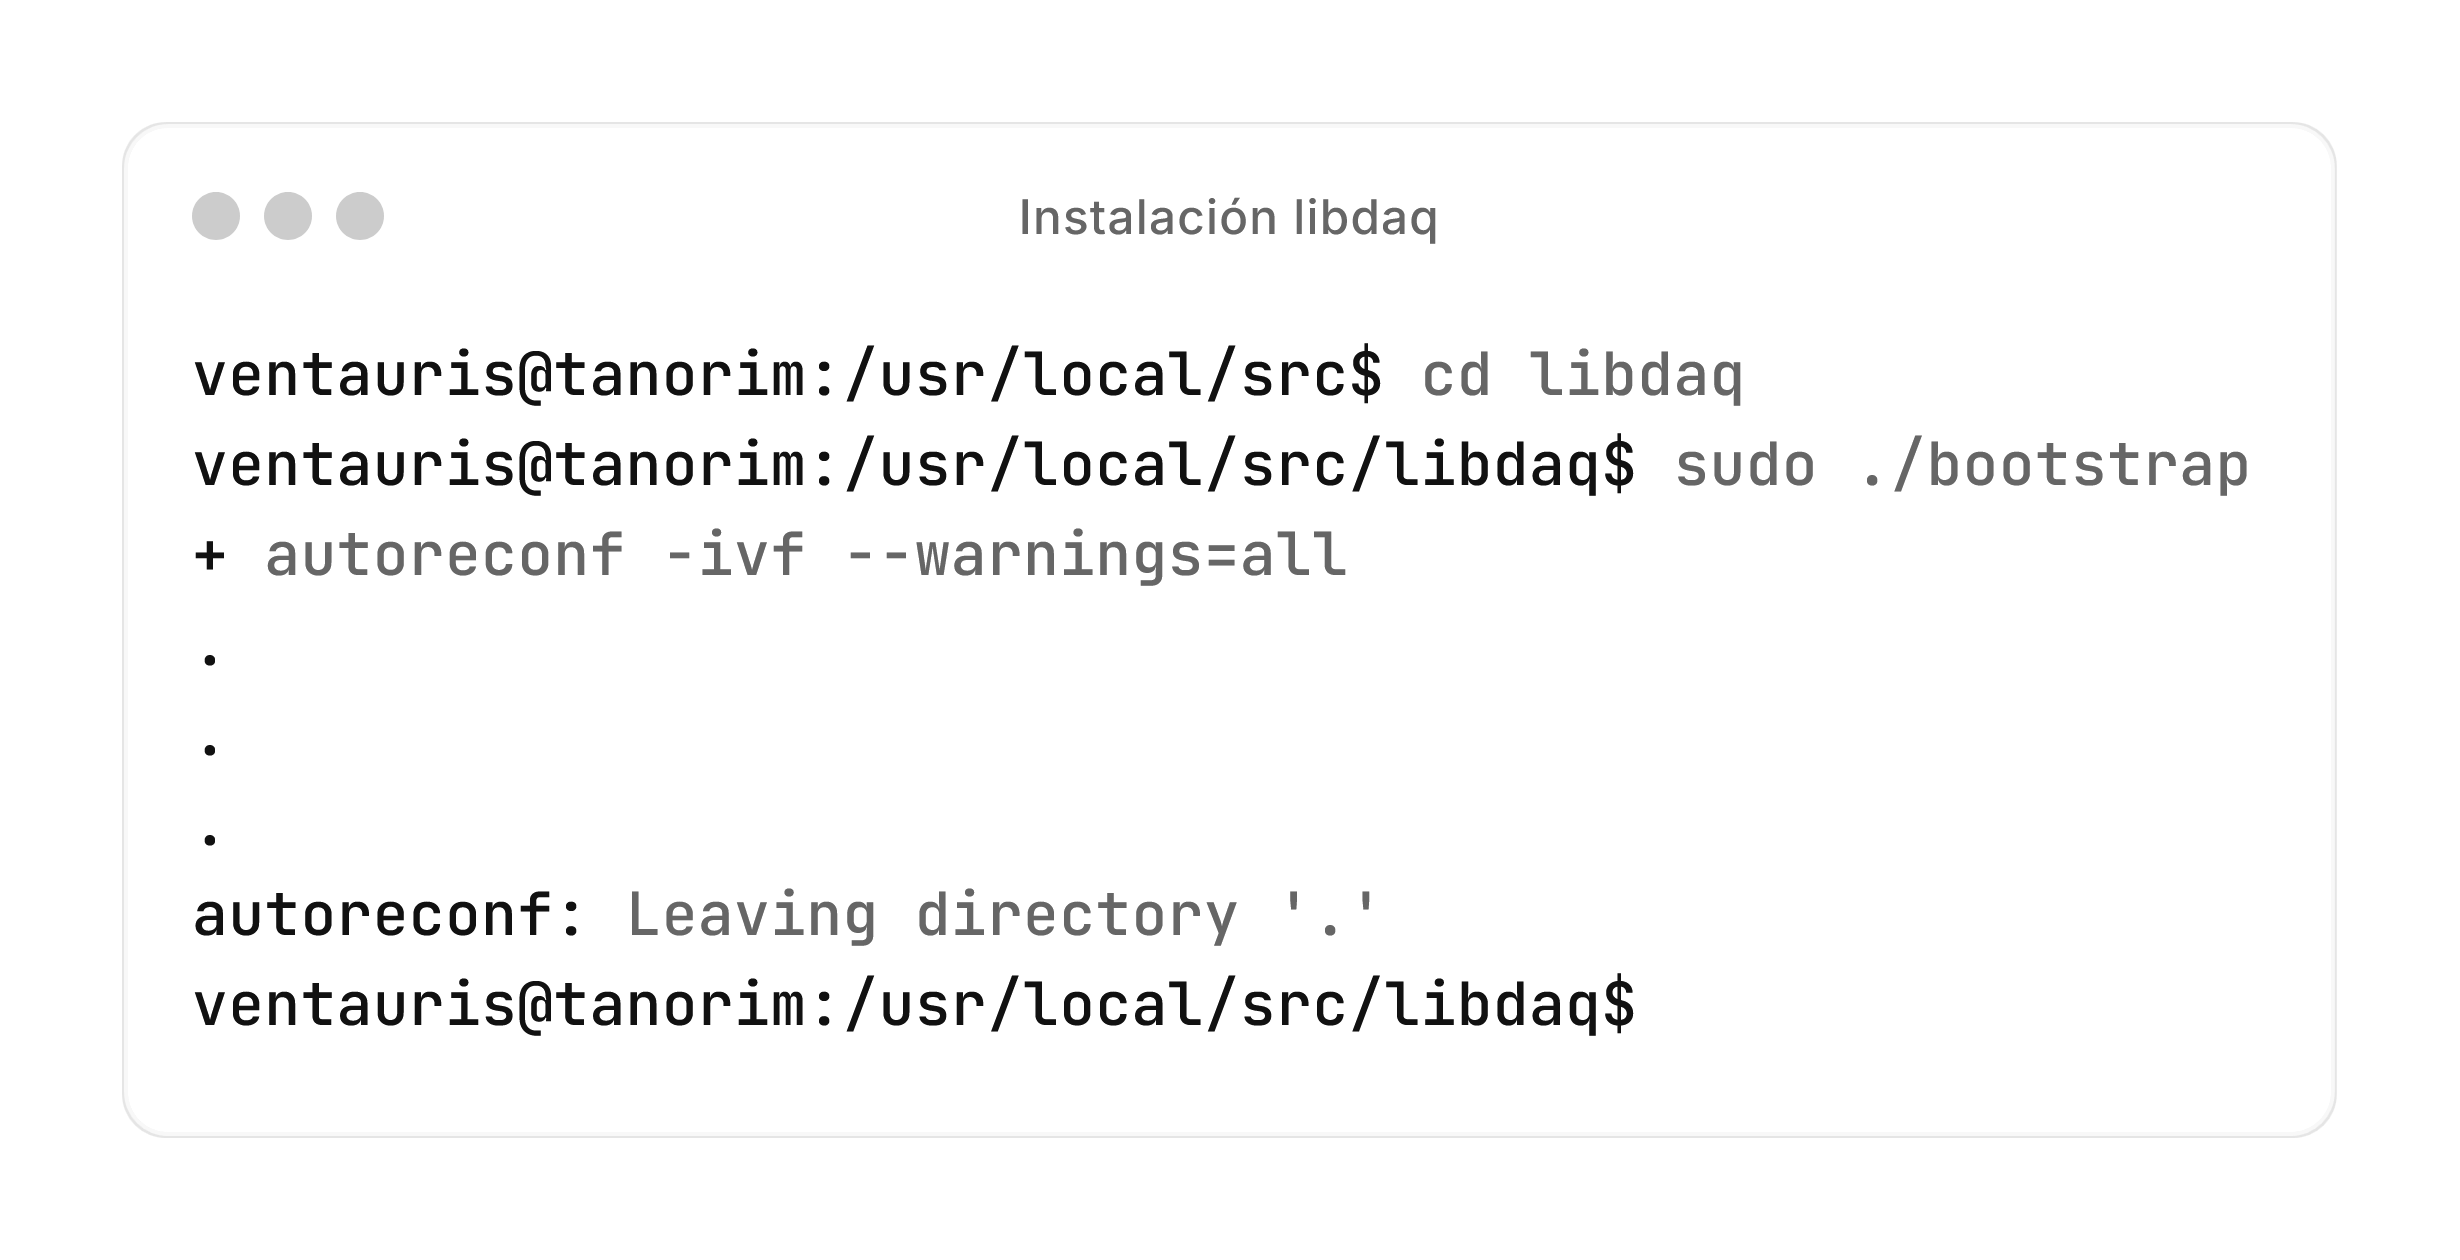
\includegraphics[scale=0.12]{instalacion_snort/10-10.png}
	\caption{Preparando \texttt{libdaq} para su compilación.}
\end{figure}

\newpage

%%%%%%%%%%%%%%%%%%%%%%%%%%%%%%%%%%%%%%%%%%%%%HECHO2%%%%%%%%%%%%%%%%%%%%%%%%%%%%%%%%%%%%%%%%%%%%%%%%%%%%%%%%%%%%%%%%%%%%%%%%%%%%%%%%%%%%%%%%%

Ejecutamos \texttt{./configure} para preparar el entorno de compilación de \texttt{libdaq}. Como se ha comentado anteriormente, este script revisa que el sistema tenga todas las dependencias necesarias y genera los archivos de configuración adecuados para compilar el software sin complicaciones.

\begin{figure}[H]
	\centering
	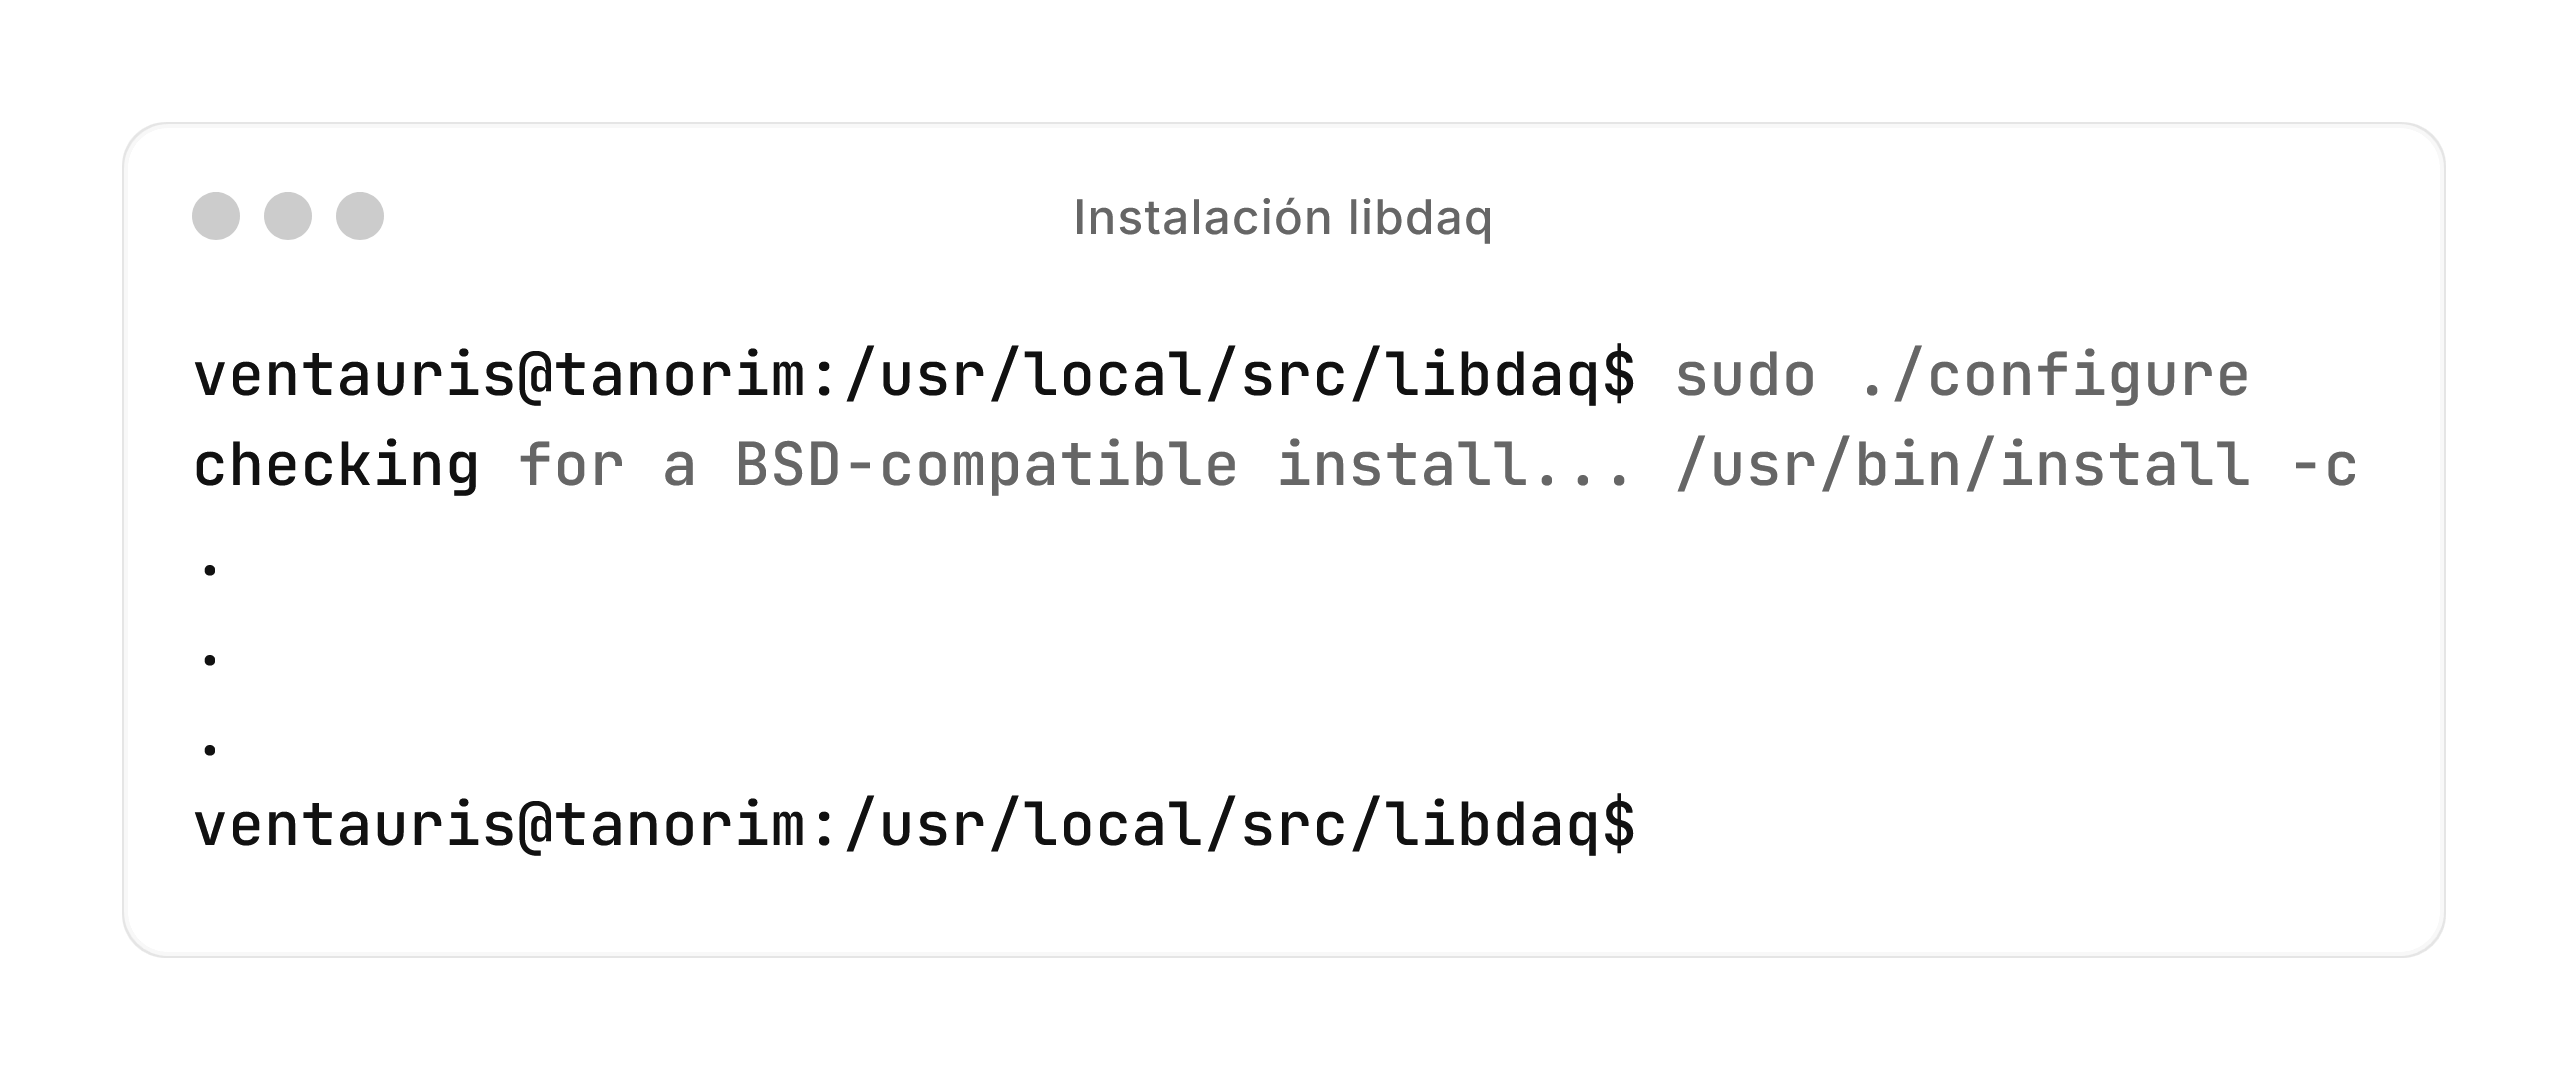
\includegraphics[scale=0.12]{instalacion_snort/11-11.png}
	\caption{Configurando \texttt{libdaq} antes de la compilación.}
\end{figure}

La ejecución de \texttt{make} llevará a cabo la compilación de \texttt{libdaq}. Este proceso traduce el código fuente a binarios ejecutables, asegurándose de que todas las dependencias y archivos necesarios se generen correctamente para su posterior instalación.

\begin{figure}[H]
	\centering
	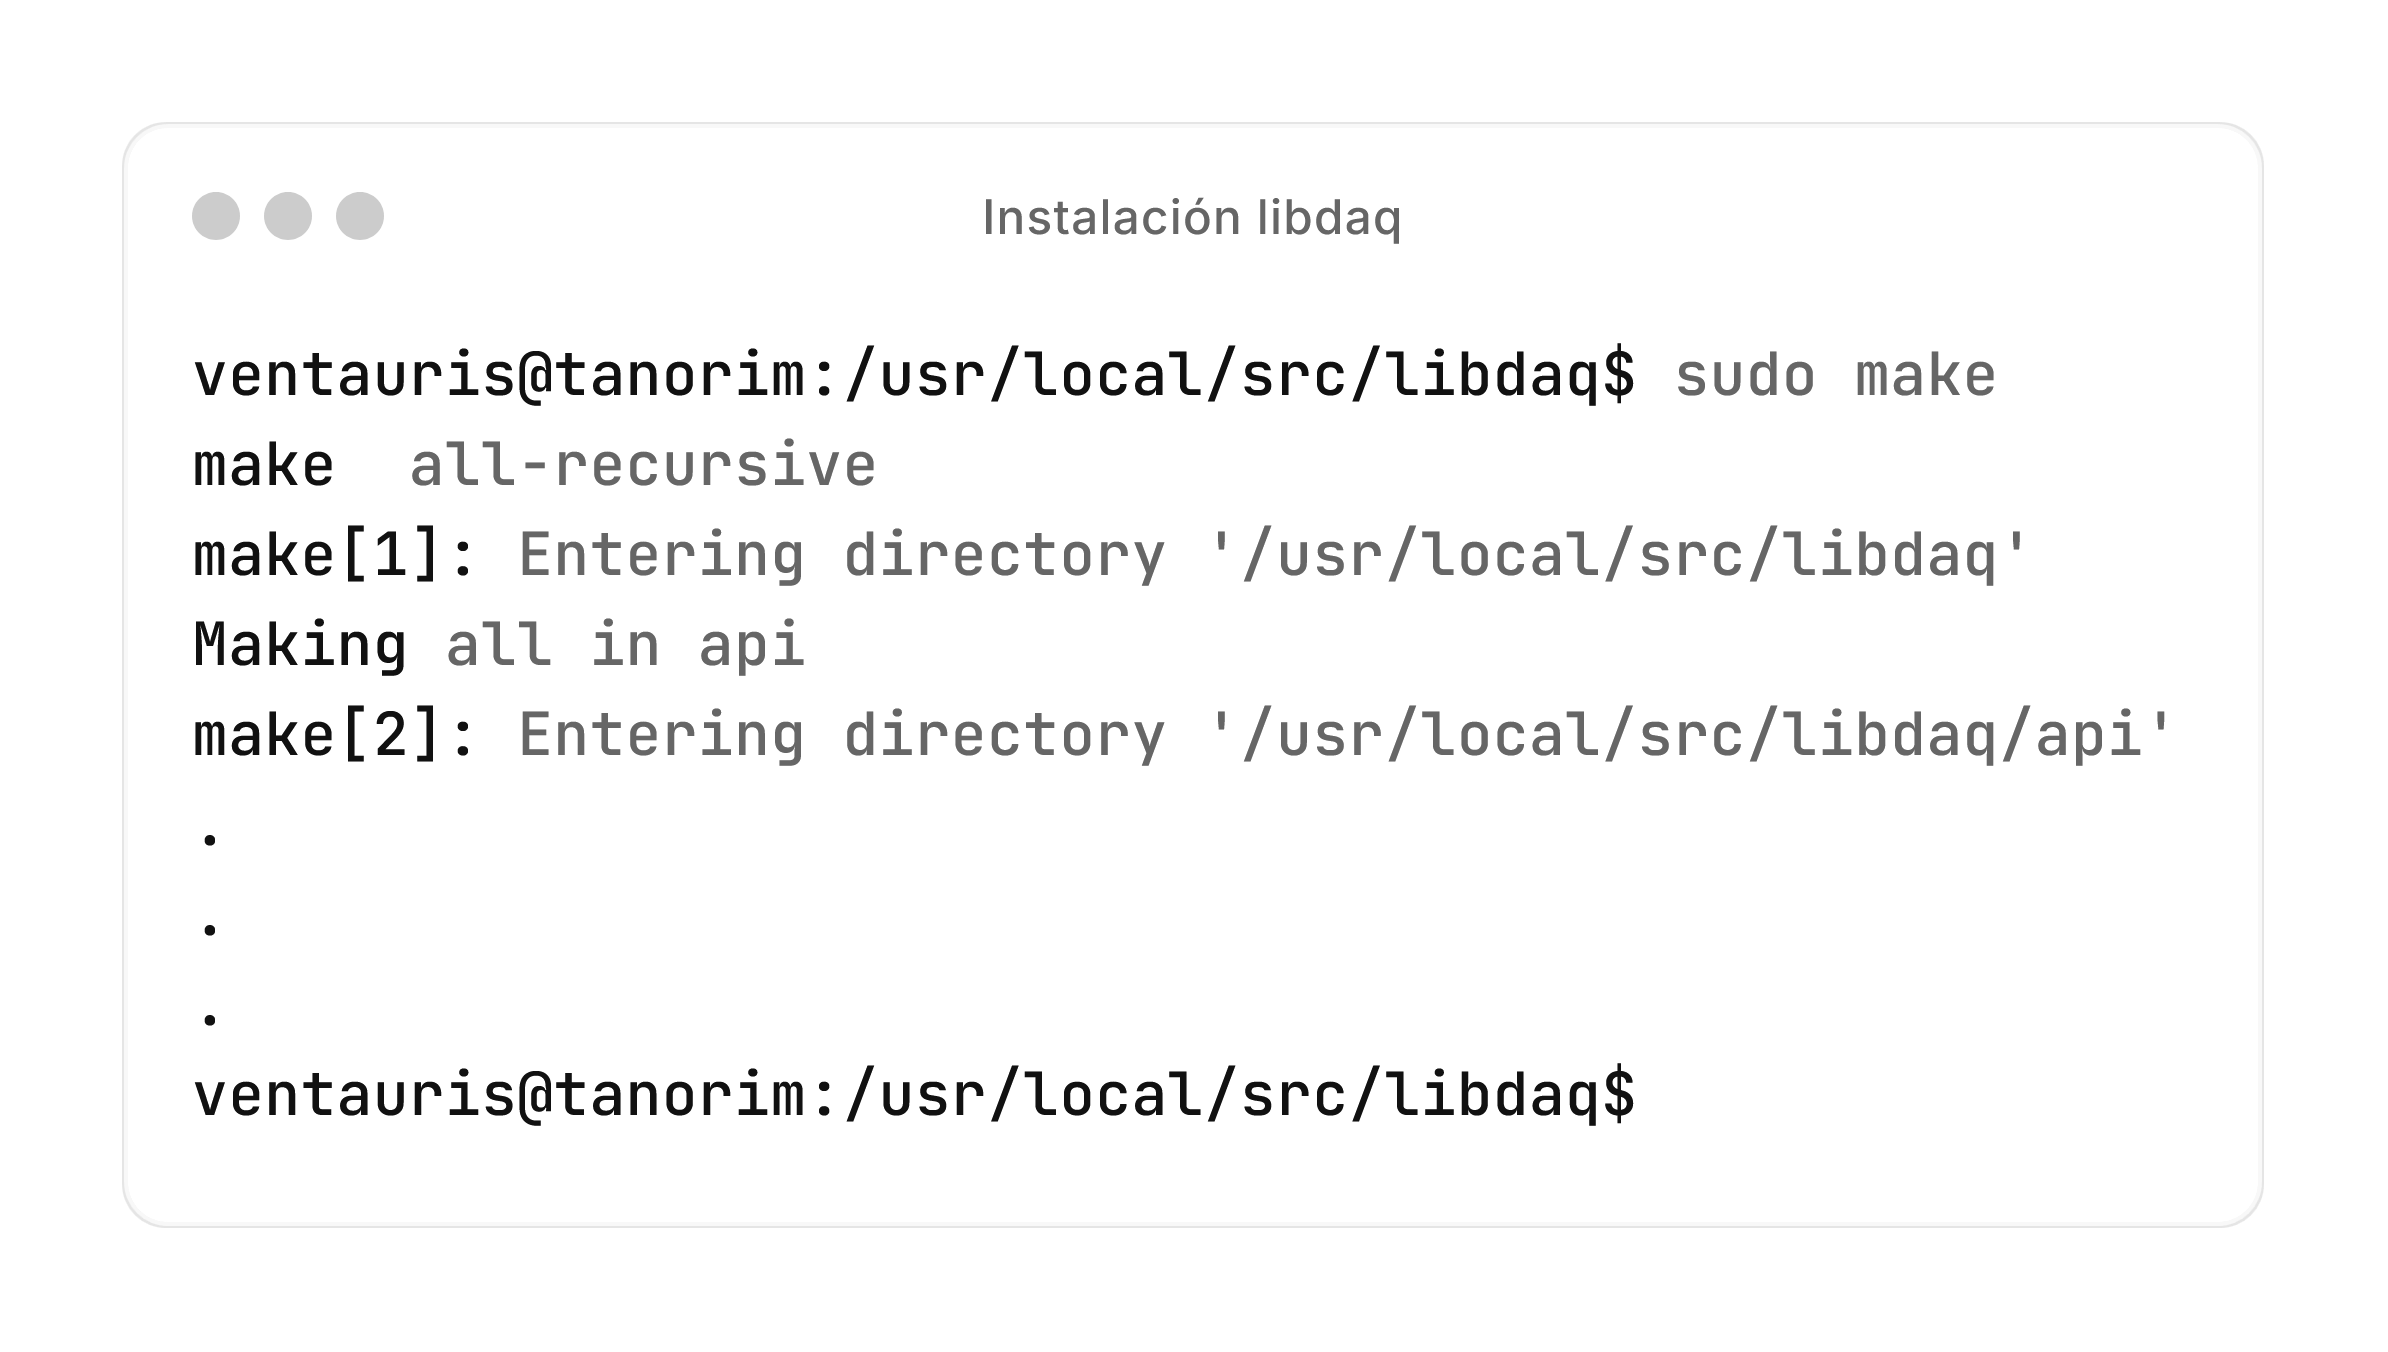
\includegraphics[scale=0.12]{instalacion_snort/12-12.png}
	\caption{Compilando \texttt{libdaq}.}
\end{figure}

\newpage

La instalación final la llevaremos a cabo mediante \texttt{sudo make install}. Esto copia los archivos compilados a sus ubicaciones correspondientes dentro del sistema para que puedan ser utilizados por \textbf{Snort} y otros programas que así lo requieran.

\begin{figure}[H]
	\centering
	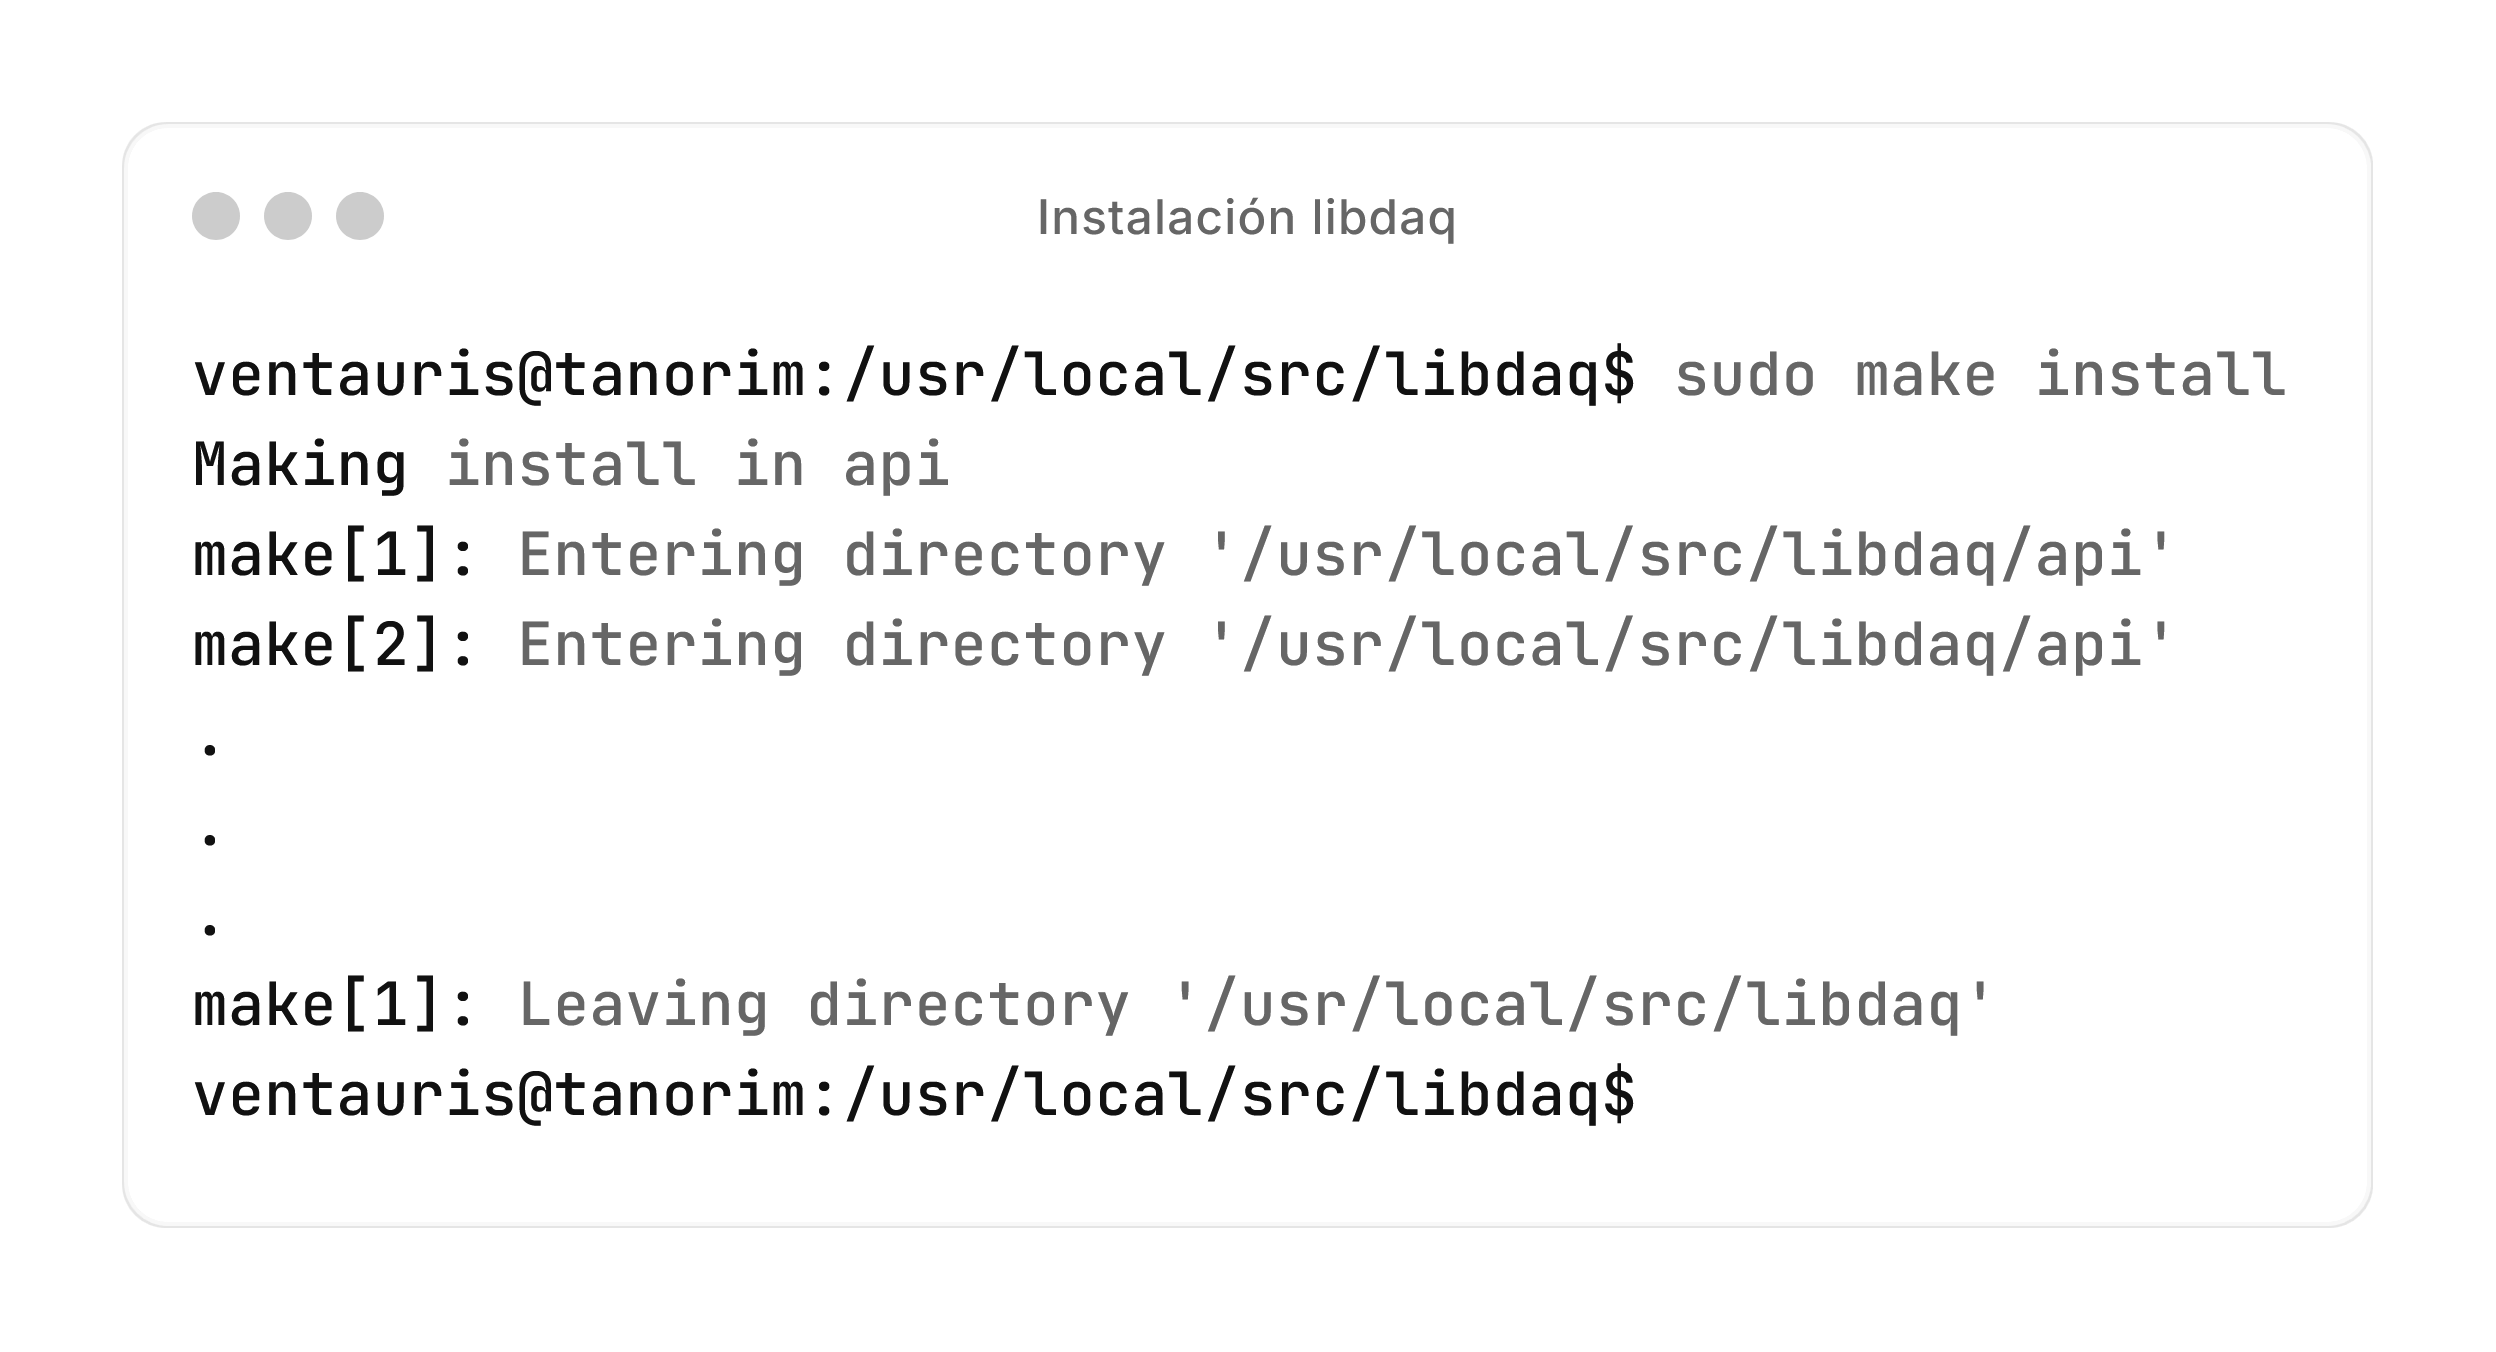
\includegraphics[scale=0.12]{instalacion_snort/13-13.png}
	\caption{Instalando \texttt{libdaq}.}
\end{figure}

Listamos los archivos de configuración de \texttt{libdaq} en \texttt{/usr/local/lib/pkgconfig/} para asegurarnos de que la instalación se haya completado correctamente. Después, exportamos la variable \texttt{PKG\_CONFIG\_PATH} para que el sistema reconozca la librería. Finalmente, usamos \texttt{pkg-config --modversion libdaq} para confirmar que la versión instalada es la \textbf{3.0.19}.

\begin{figure}[H]
	\centering
	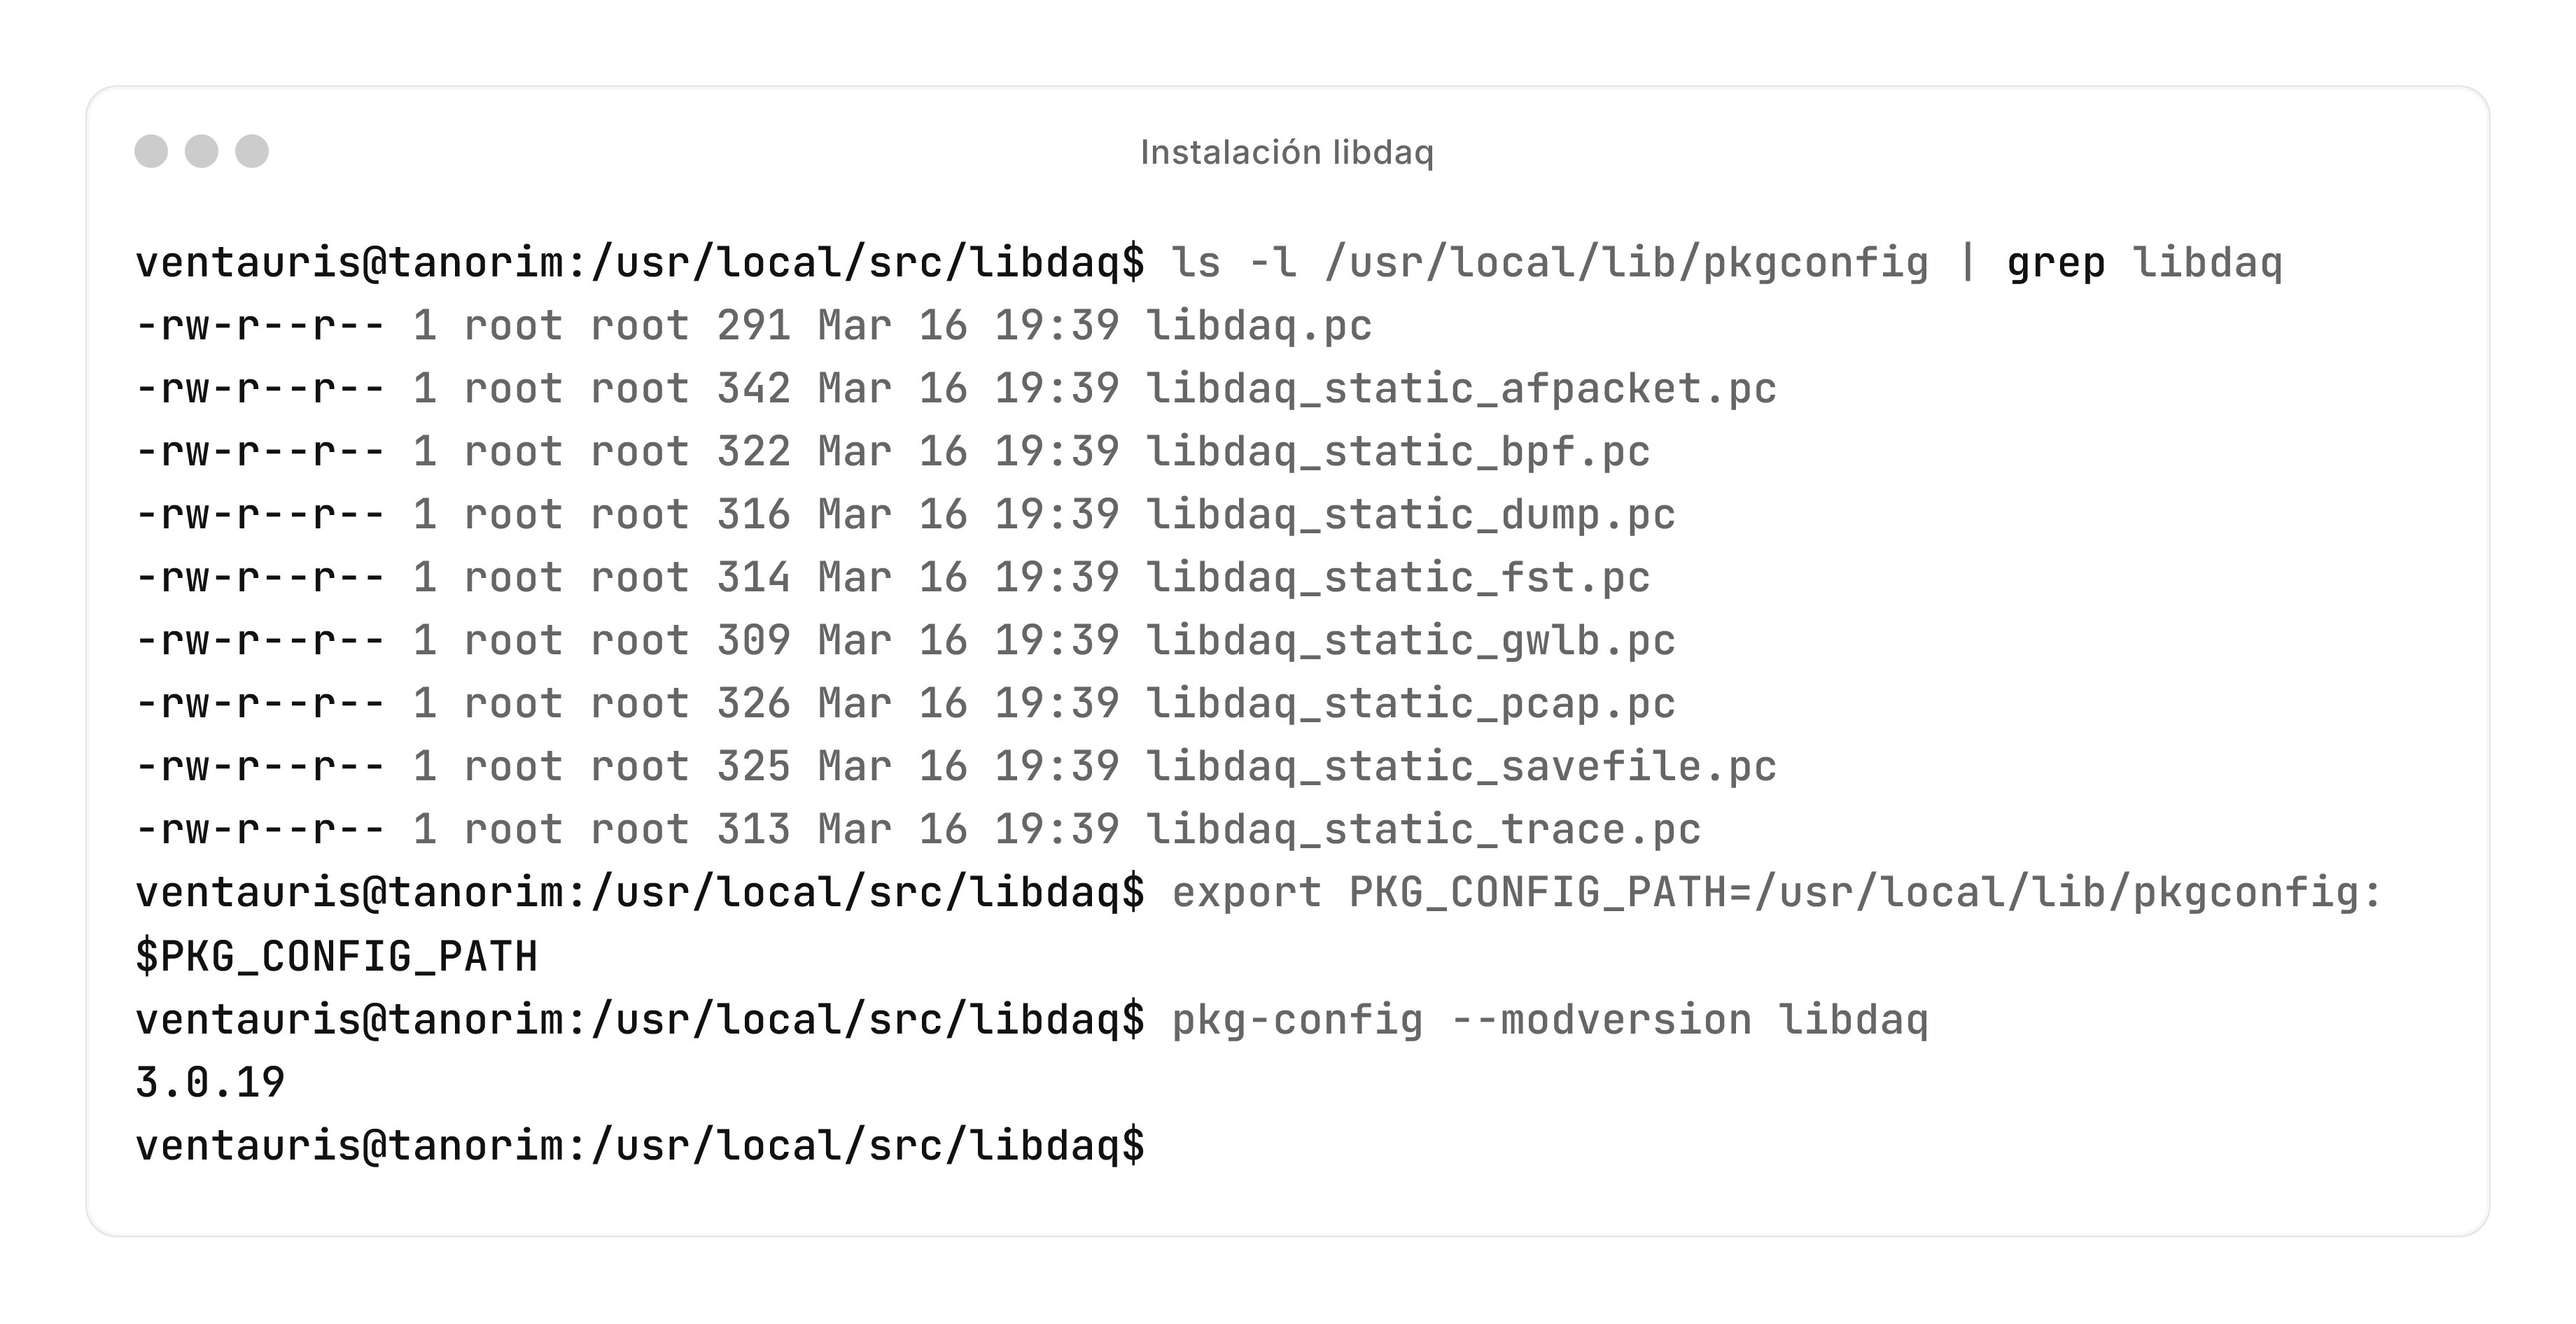
\includegraphics[scale=0.12]{instalacion_snort/14-14.png}
	\caption{Verificando la instalación de \texttt{libdaq}.}
\end{figure}

\newpage

\subsubsection*{Instalación de la dependencia libhwloc-dev}

Instalamos \texttt{libhwloc-dev}, una librería necesaria para la ejecución de \textbf{Snort 3} y sus dependencias. Se incluyen automáticamente otros paquetes adicionales como \texttt{libhwloc-plugins}, \texttt{libnuma-dev} y \texttt{libpciaccess0}, que ayudan en la gestión de hardware y optimización del rendimiento.

\begin{figure}[H]
	\centering
	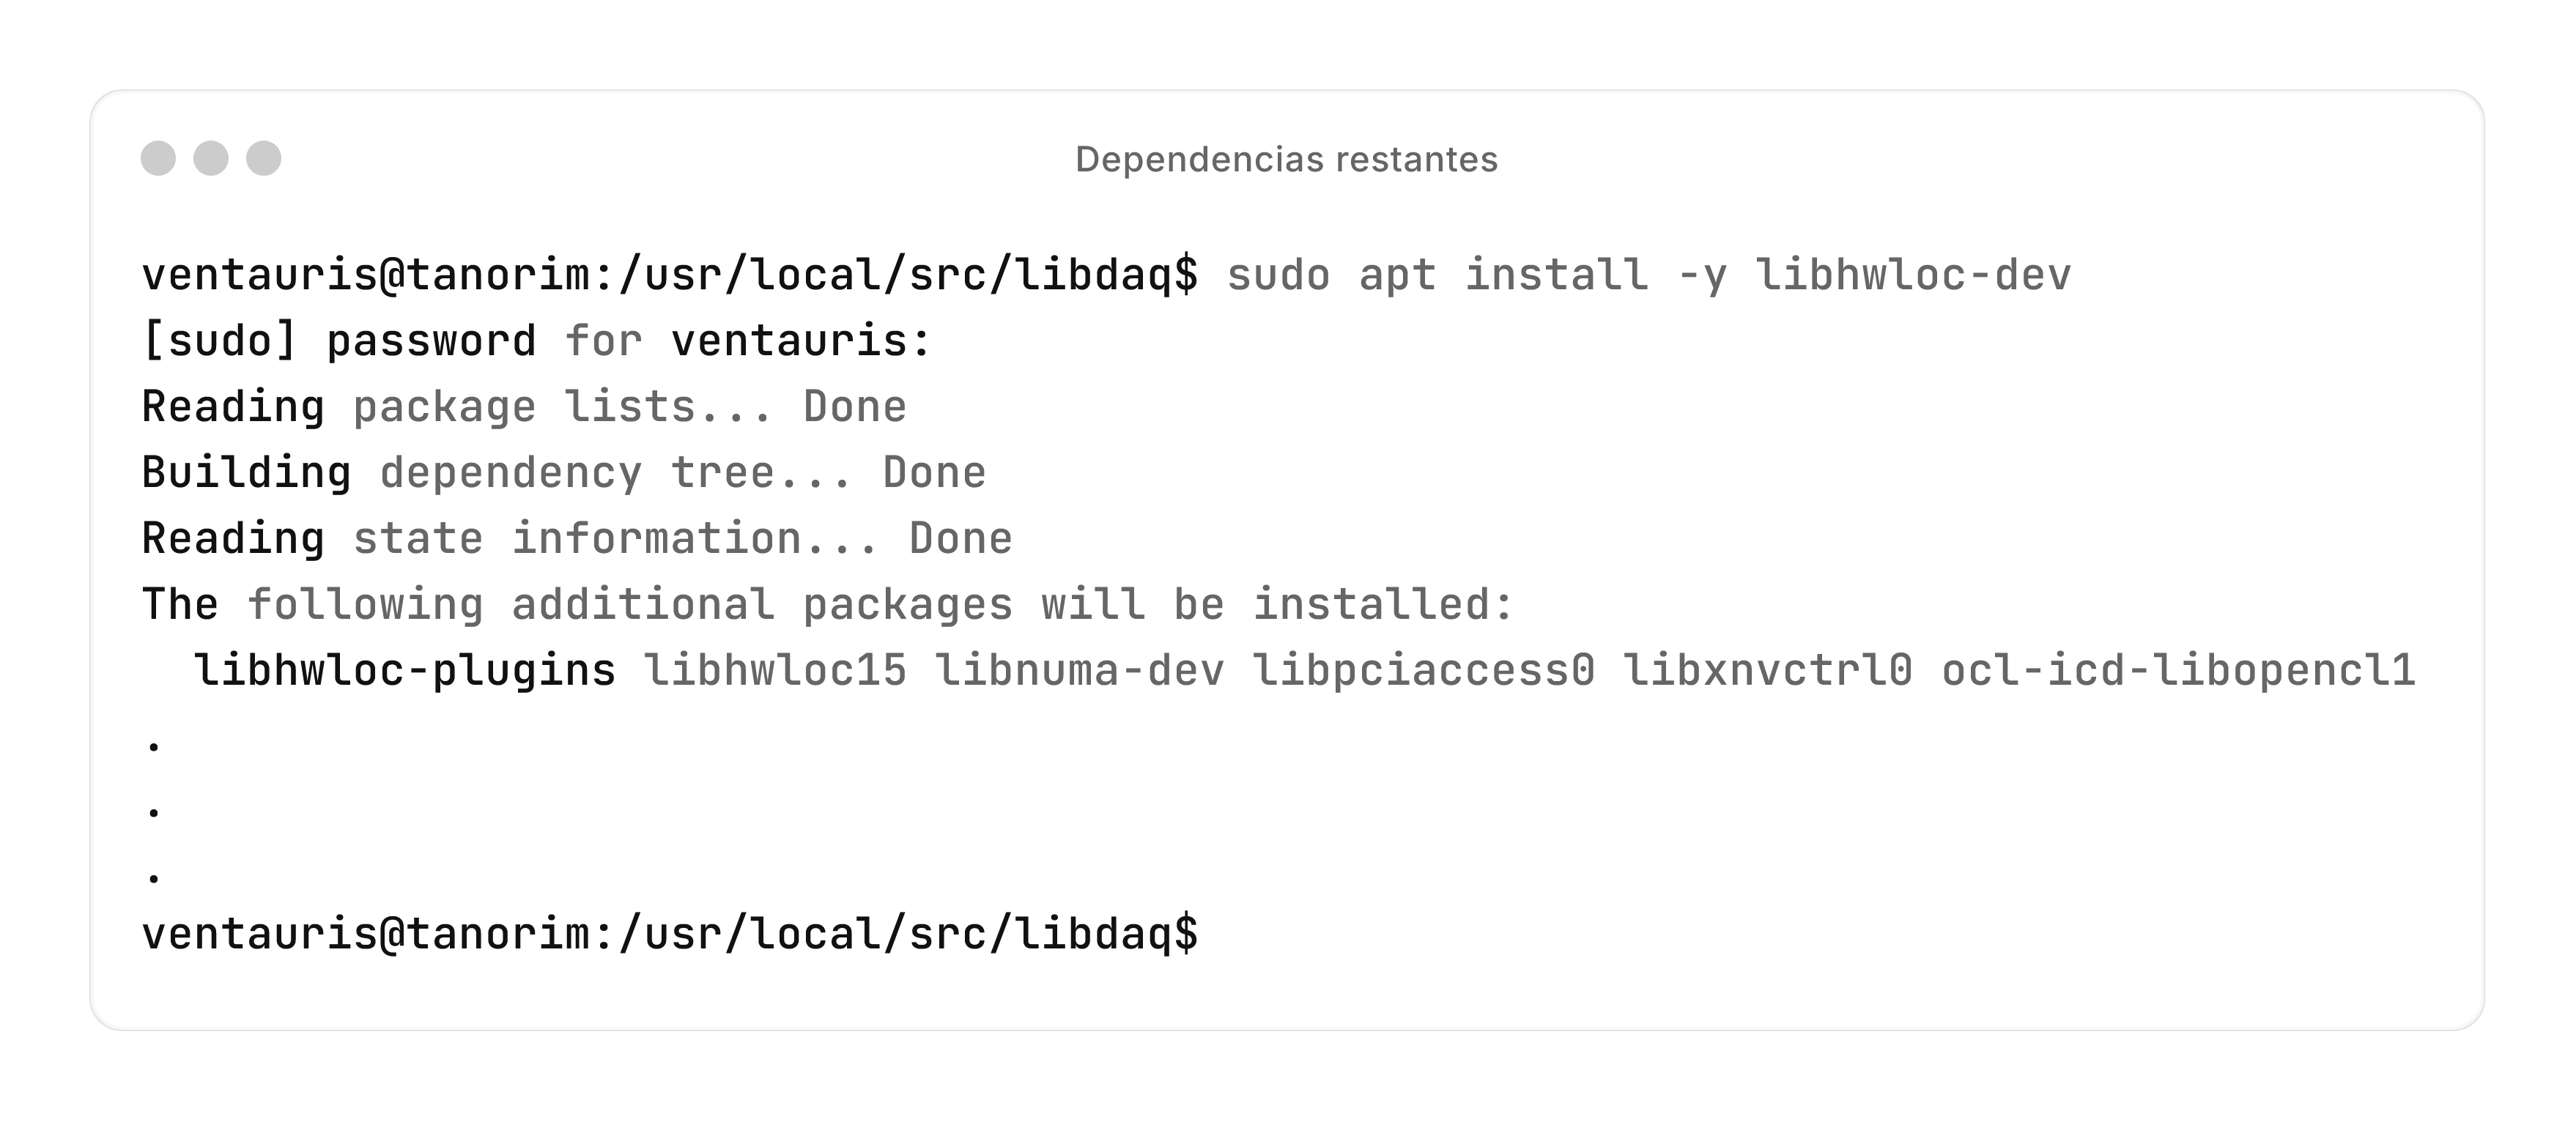
\includegraphics[scale=0.12]{instalacion_snort/15-15.png}
	\caption{Instalando dependencias necesarias.}
\end{figure}

\subsubsection*{Instalación de la dependencia libluajit}

Aquí instalamos \texttt{libluajit-5.1-dev}, más dependencias para \textbf{Snort 3}, ya que utiliza \textbf{LuaJIT} para la configuración y personalización de reglas. También se instalan automáticamente \texttt{libluajit-5.1-2} y \texttt{libluajit-5.1-common}, que contienen las bibliotecas compartidas necesarias para funcionar correctamente.

\begin{figure}[H]
	\centering
	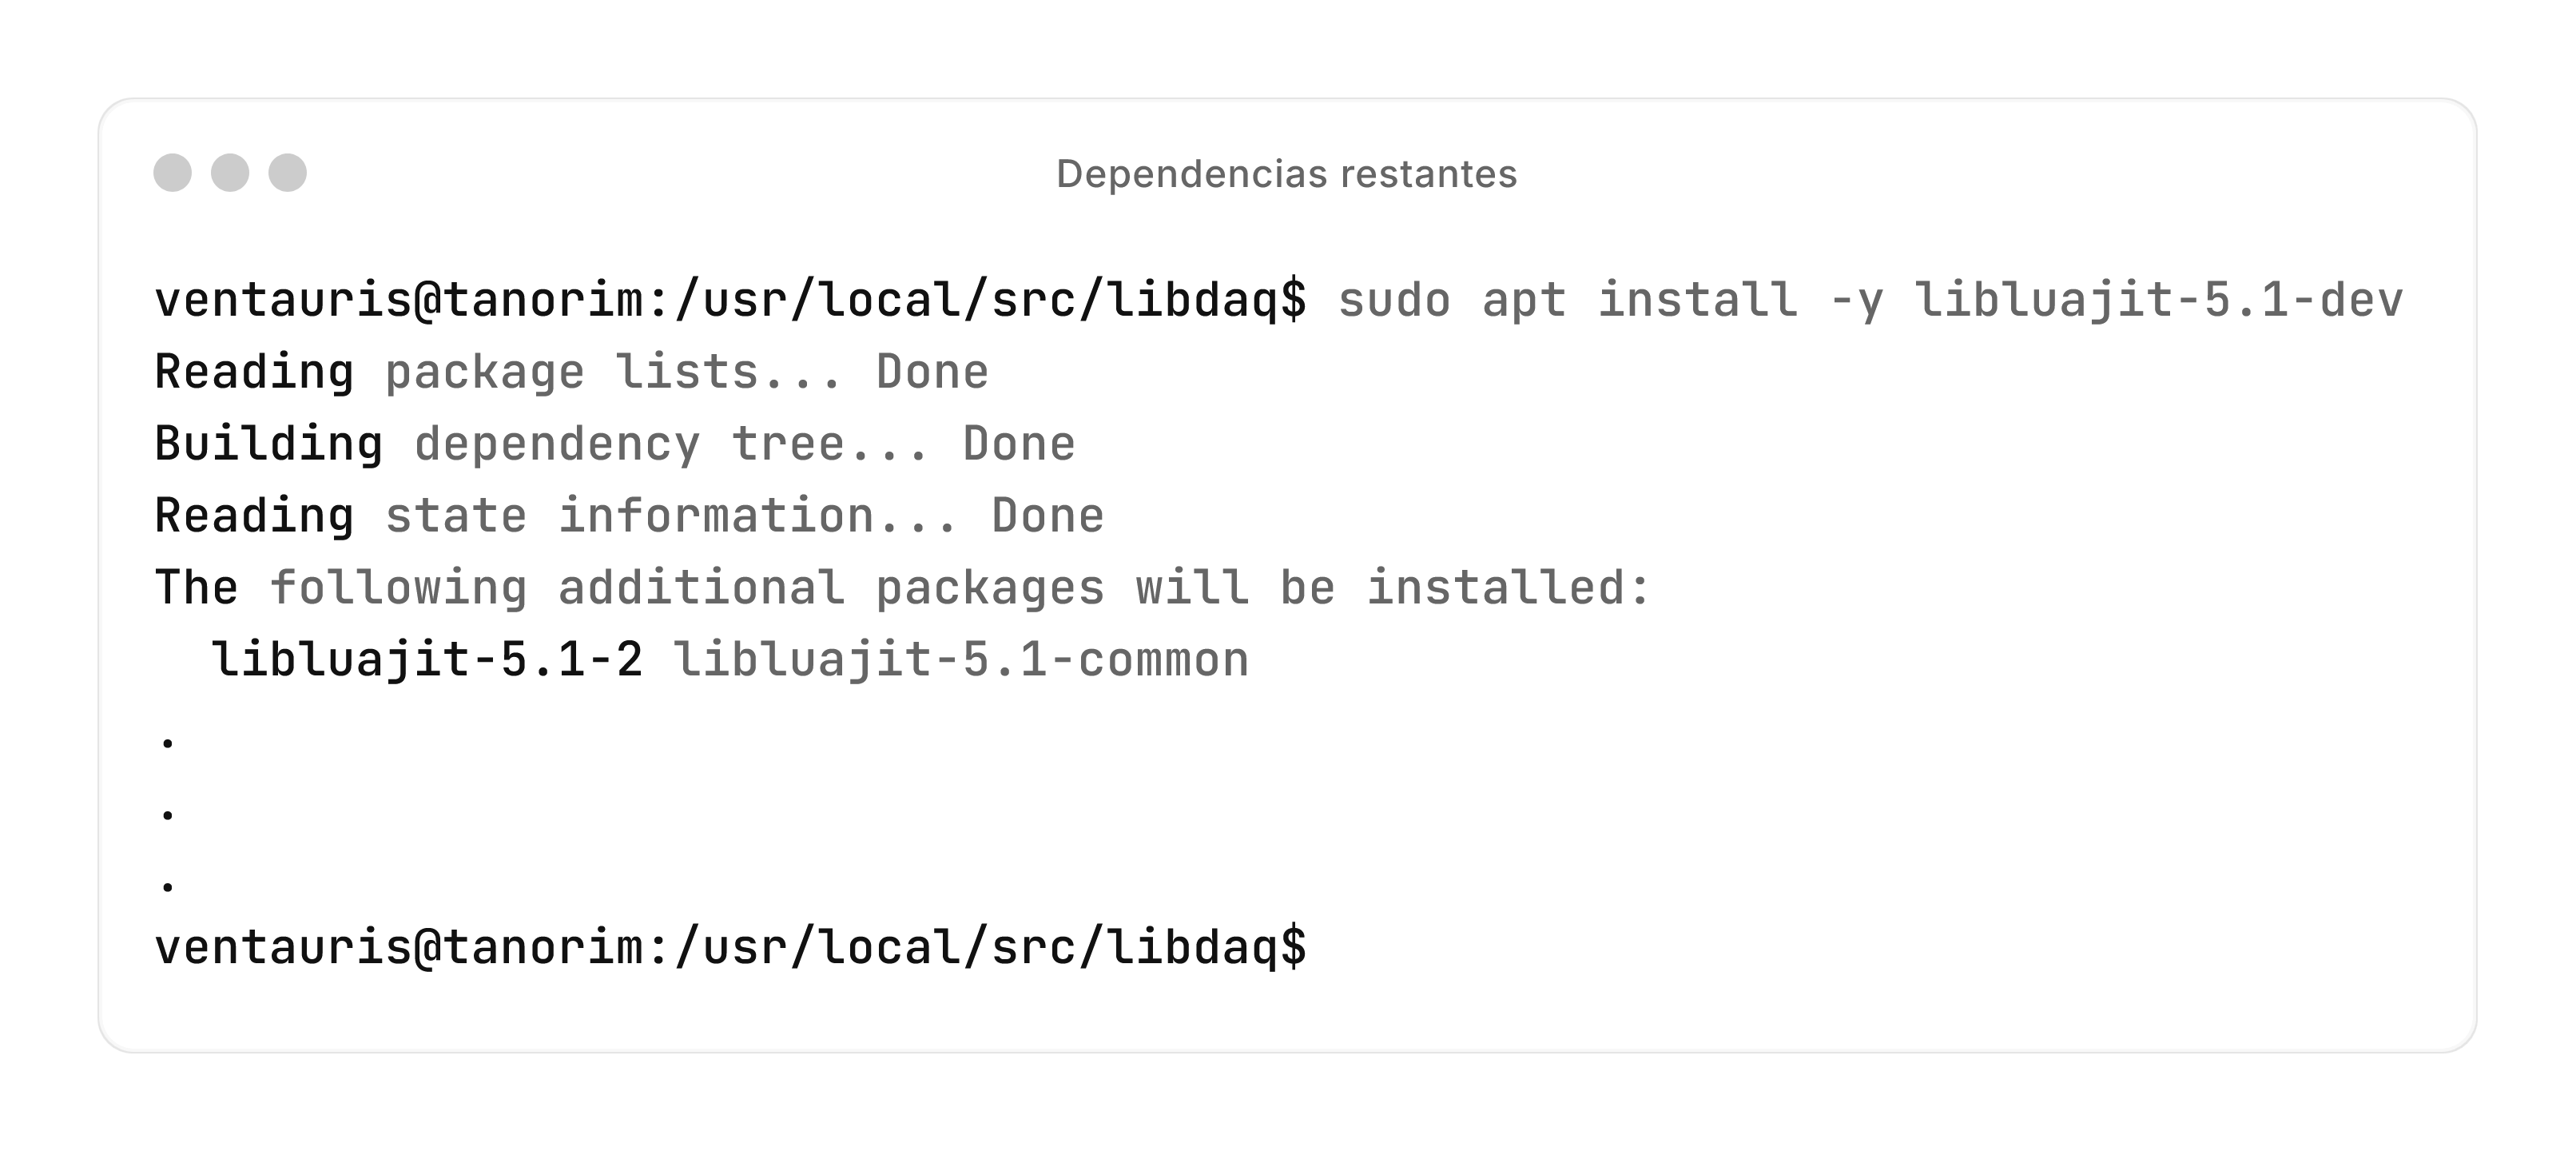
\includegraphics[scale=0.12]{instalacion_snort/16-16.png}
	\caption{Instalando \textbf{LuaJIT} para Snort.}
\end{figure}

\newpage

\subsubsection*{Instalación de Flex y Bison}

Instalamos \texttt{Flex} y \texttt{Bison}, dos herramientas para el análisis léxico y sintáctico en la compilación de Snort. Después de la instalación, verificamos la versión de \texttt{Flex} con \texttt{flex --version} para asegurarnos de que se instaló correctamente.

\begin{figure}[H]
	\centering
	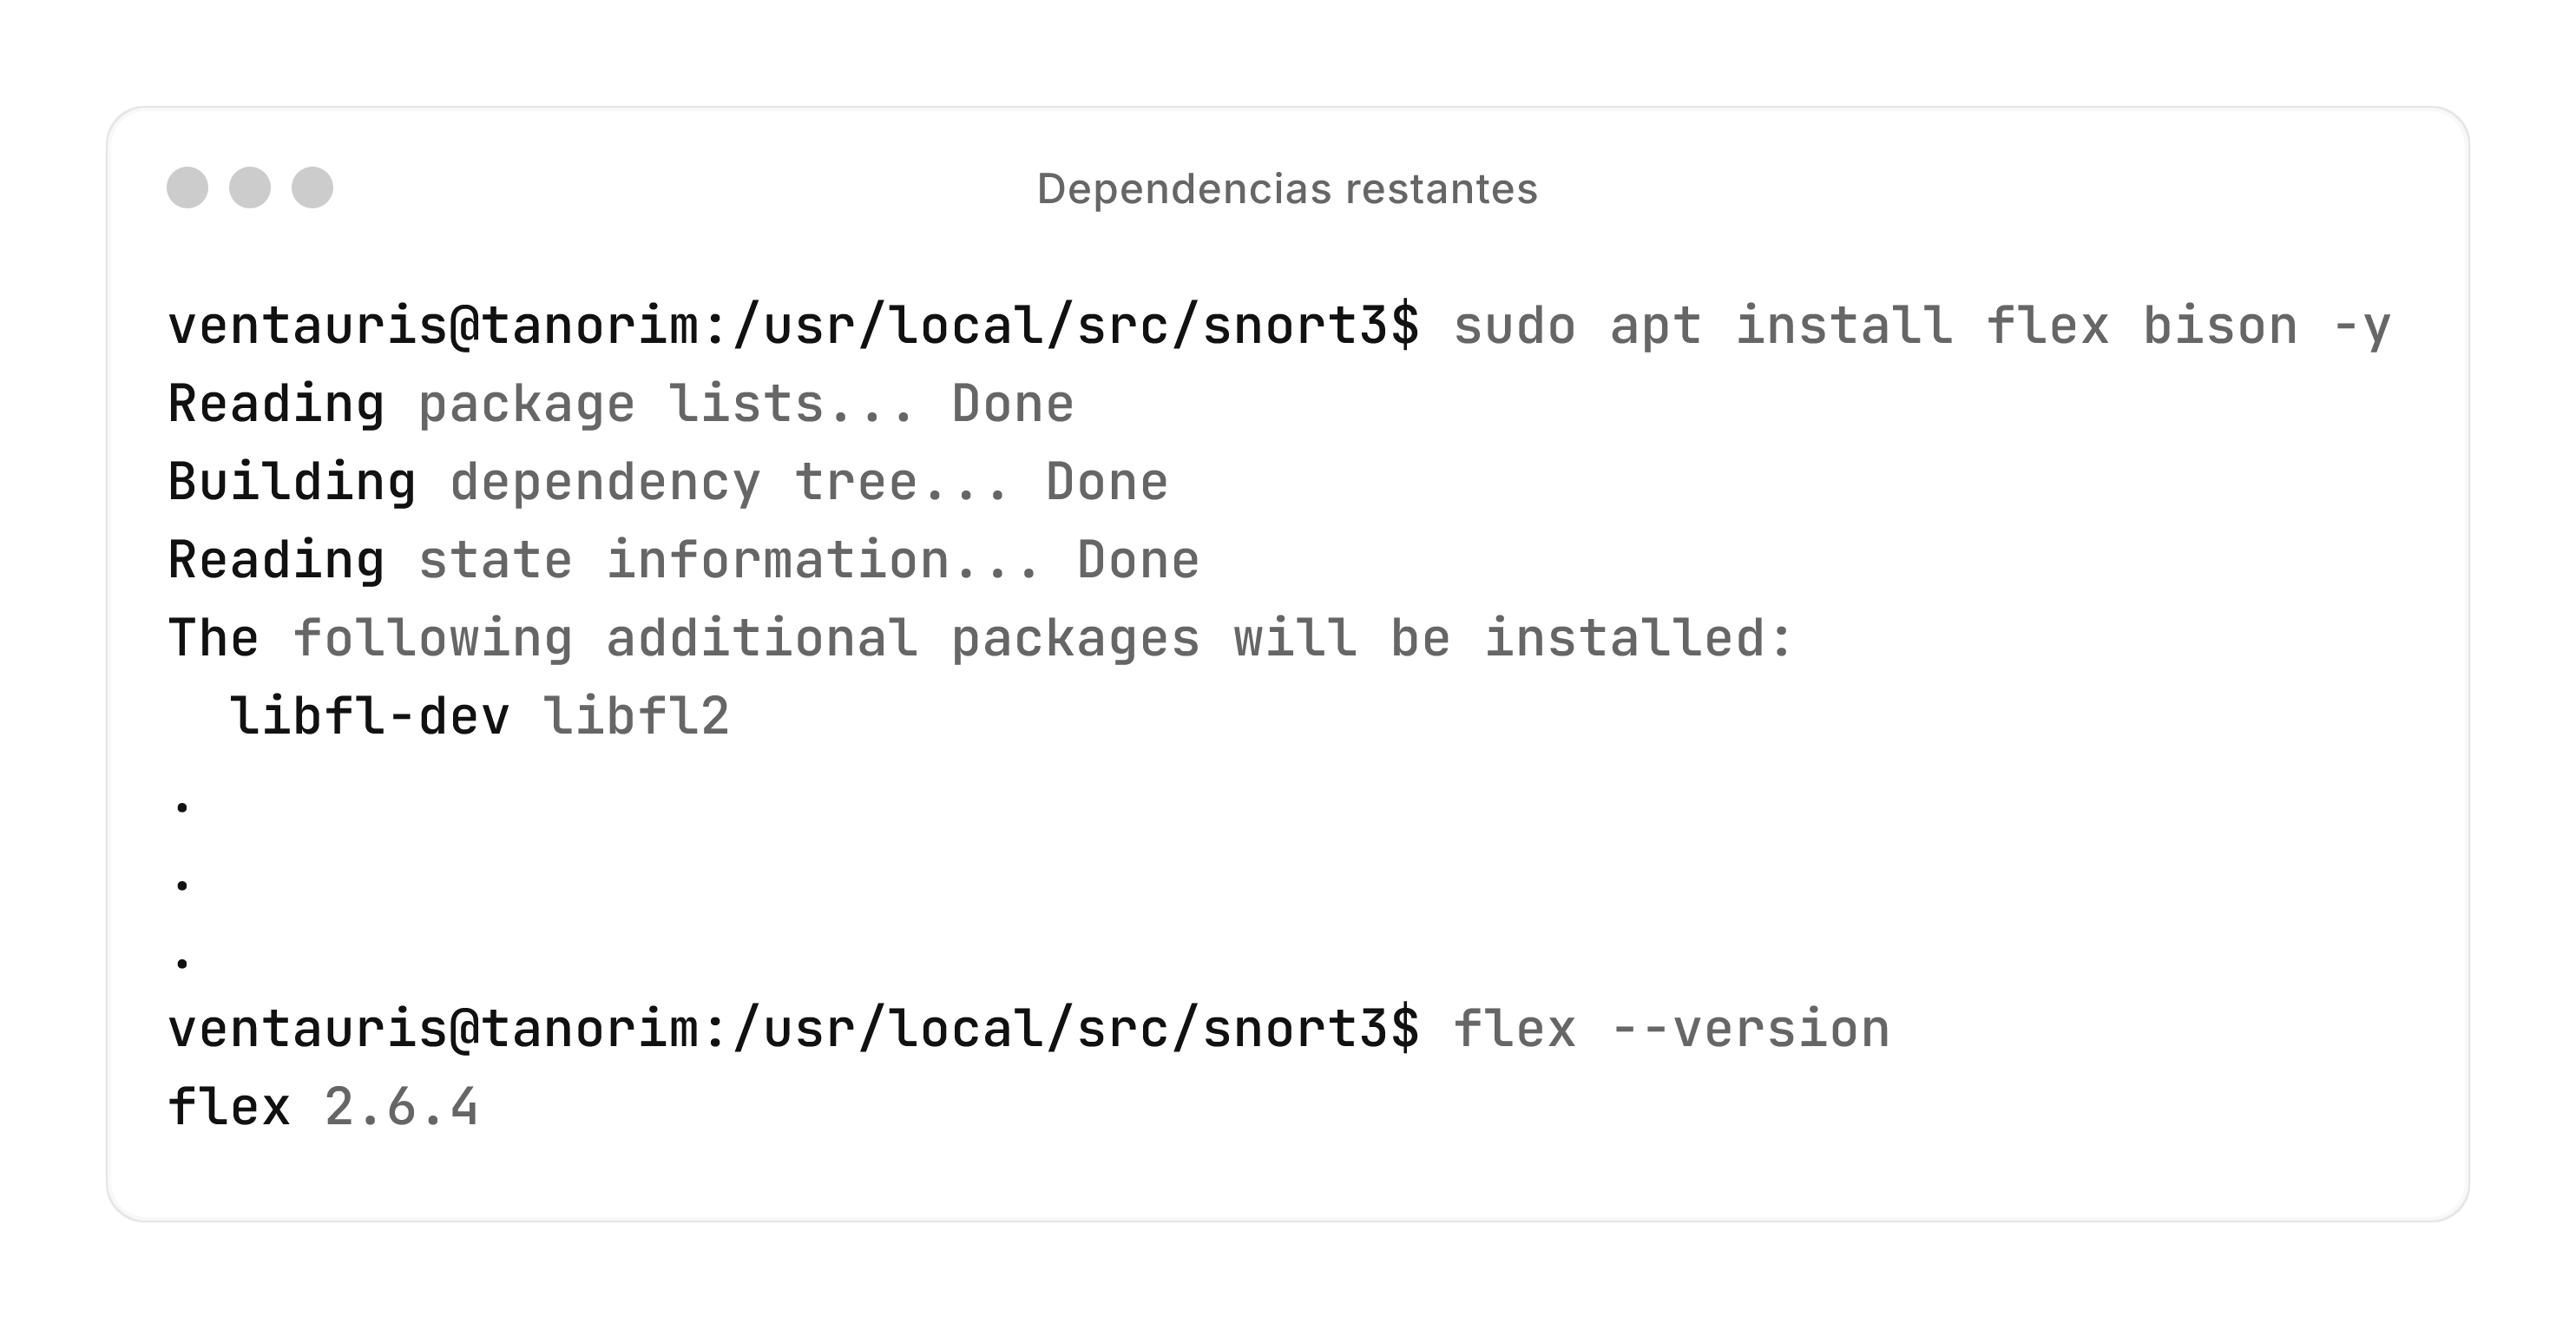
\includegraphics[scale=0.12]{instalacion_snort/19-19.png}
	\caption{Instalando \texttt{Flex} y \texttt{Bison}, herramientas necesarias para la compilación.}
\end{figure}

En este paso, instalamos \texttt{libpcre2-dev}, una biblioteca para el manejo de expresiones regulares en \textbf{Snort 3}. Nos es útil para la detección de patrones en el tráfico de red.

\begin{figure}[H]
	\centering
	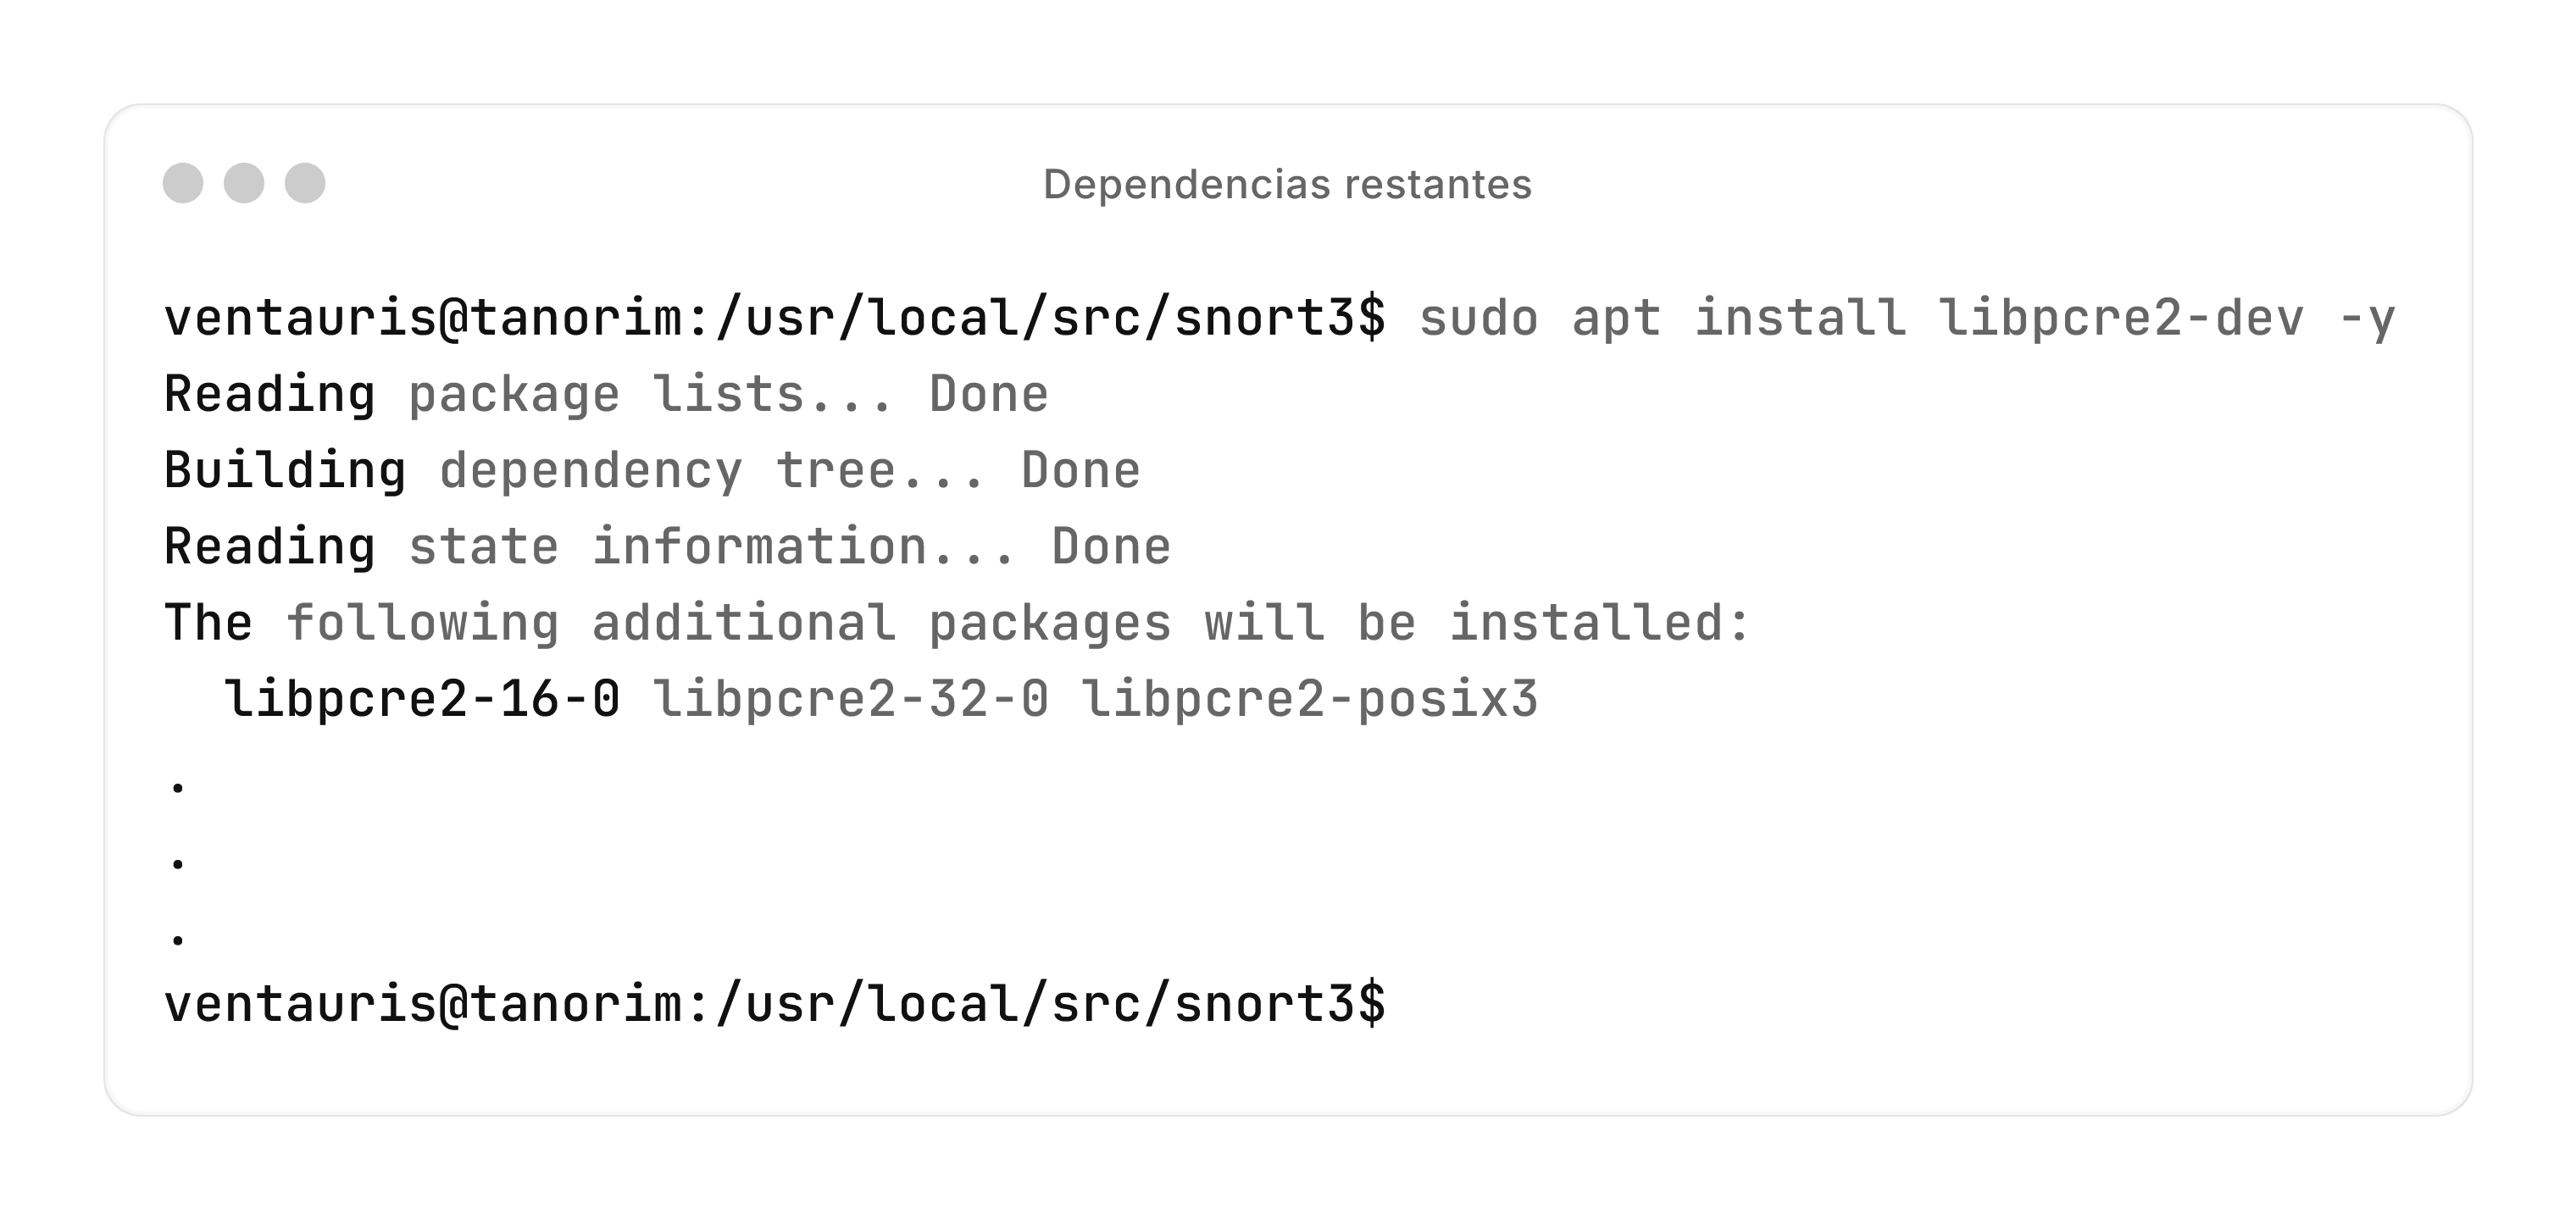
\includegraphics[scale=0.12]{instalacion_snort/20-20.png}
	\caption{Instalando la biblioteca \texttt{PCRE2} para el manejo de expresiones regulares.}
\end{figure}

\newpage

\subsubsection*{Clonación y compilación del código fuente de Snort}

Descargamos el código fuente de \textbf{Snort 3} directamente desde su repositorio oficial en GitHub mediante \texttt{git clone}.

\begin{figure}[H]
	\centering
	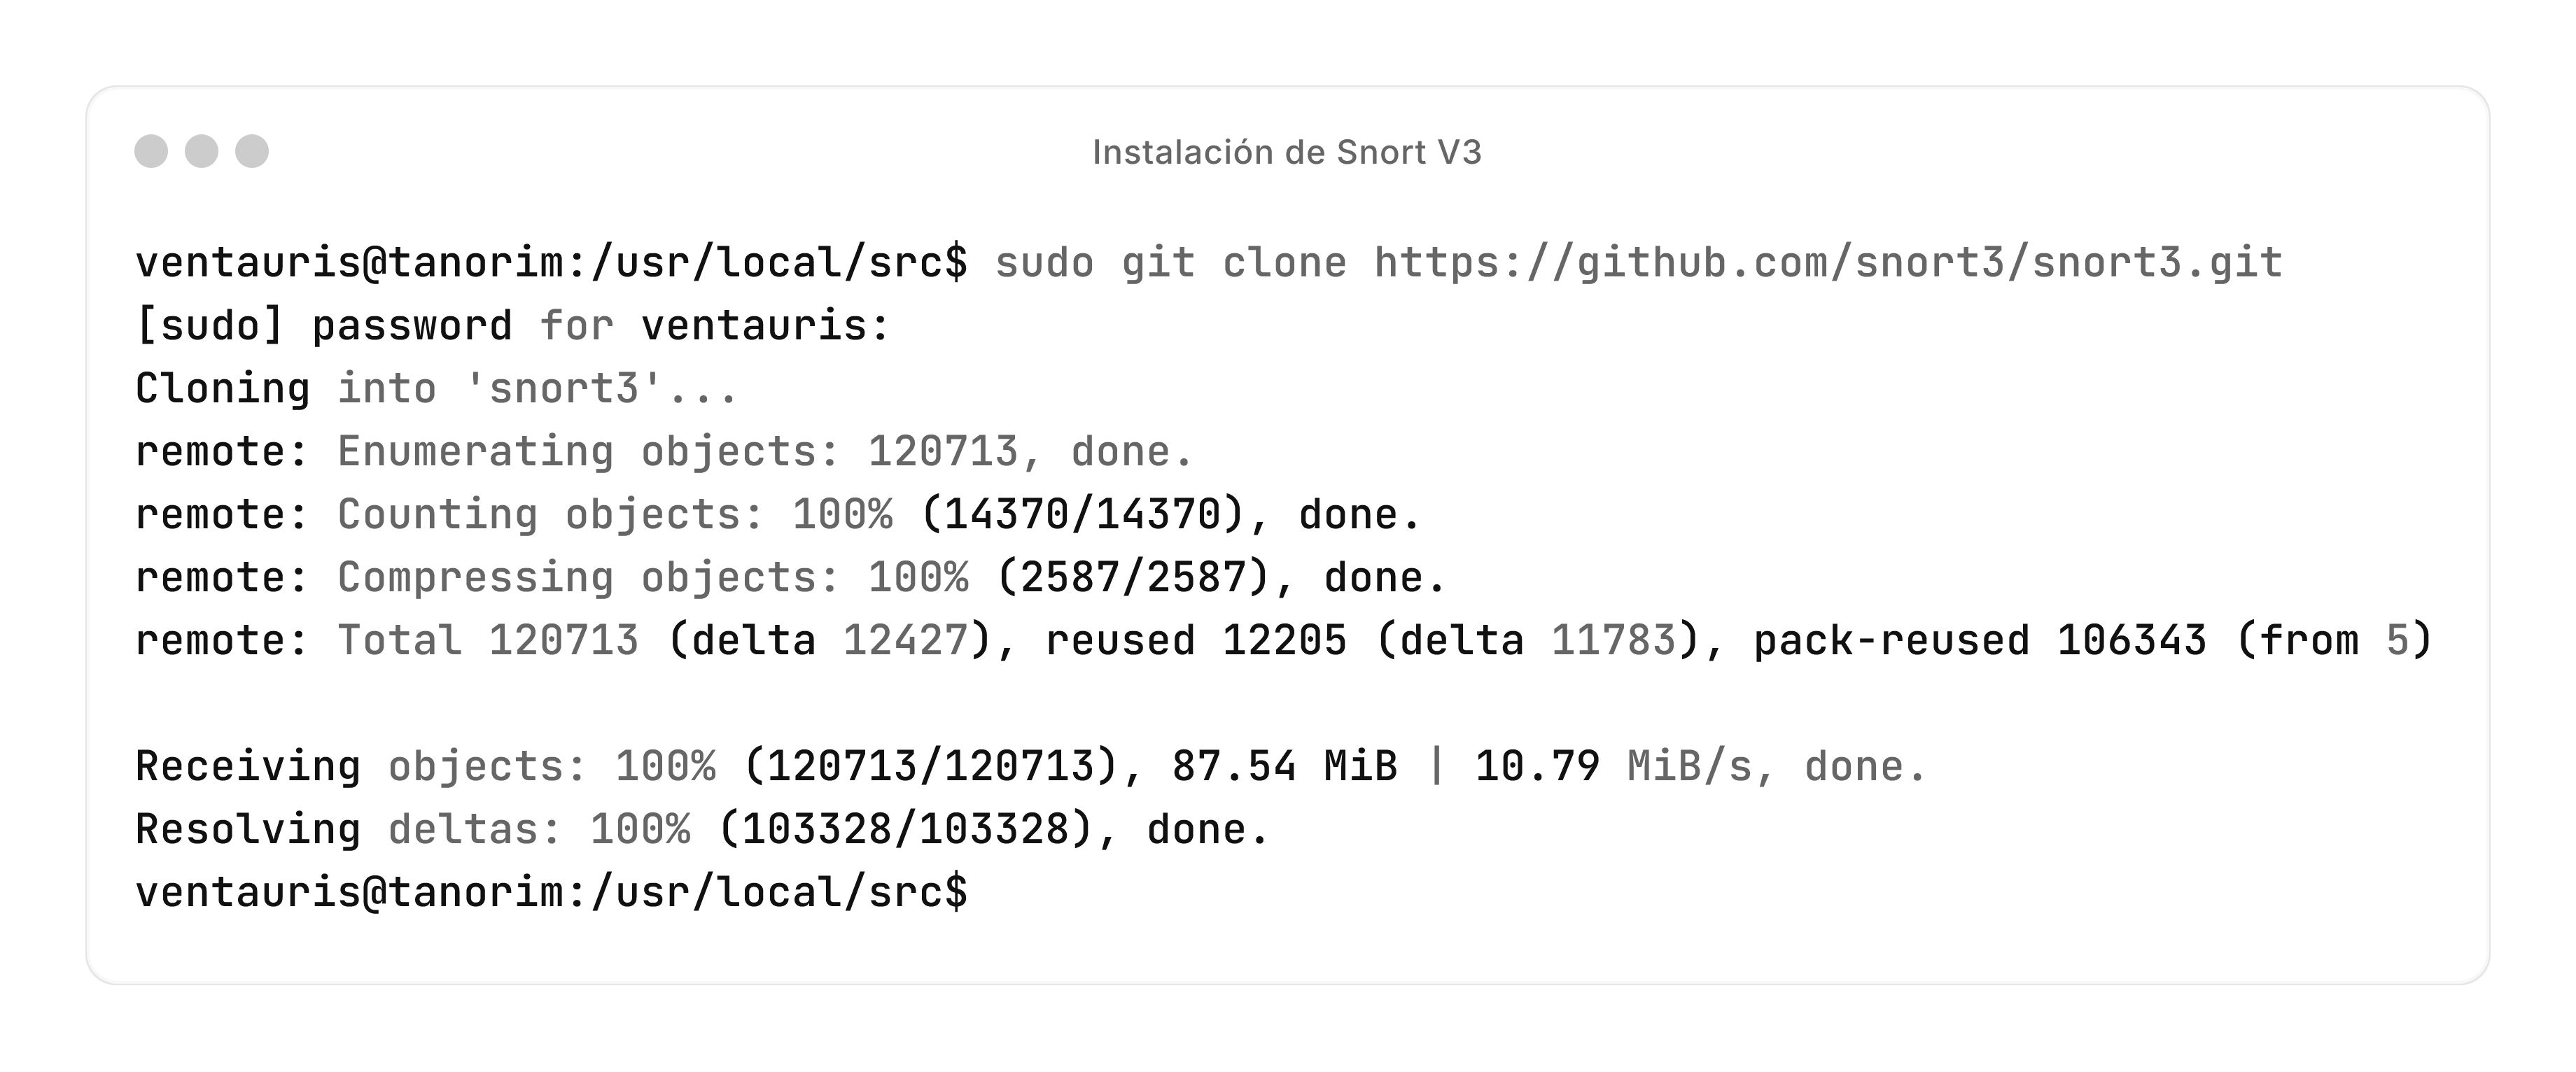
\includegraphics[scale=0.12]{instalacion_snort/17-17.png}
	\caption{Clonando el repositorio de Snort 3.}
\end{figure}

Aquí establecemos la variable \texttt{my\_path} para definir el directorio de instalación de Snort. Luego, agregamos esta configuración al archivo \texttt{~/.bashrc} para que se cargue automáticamente en futuras sesiones. Finalmente, usamos \texttt{source ~/.bashrc} para aplicar los cambios de inmediato.

\begin{figure}[H]
	\centering
	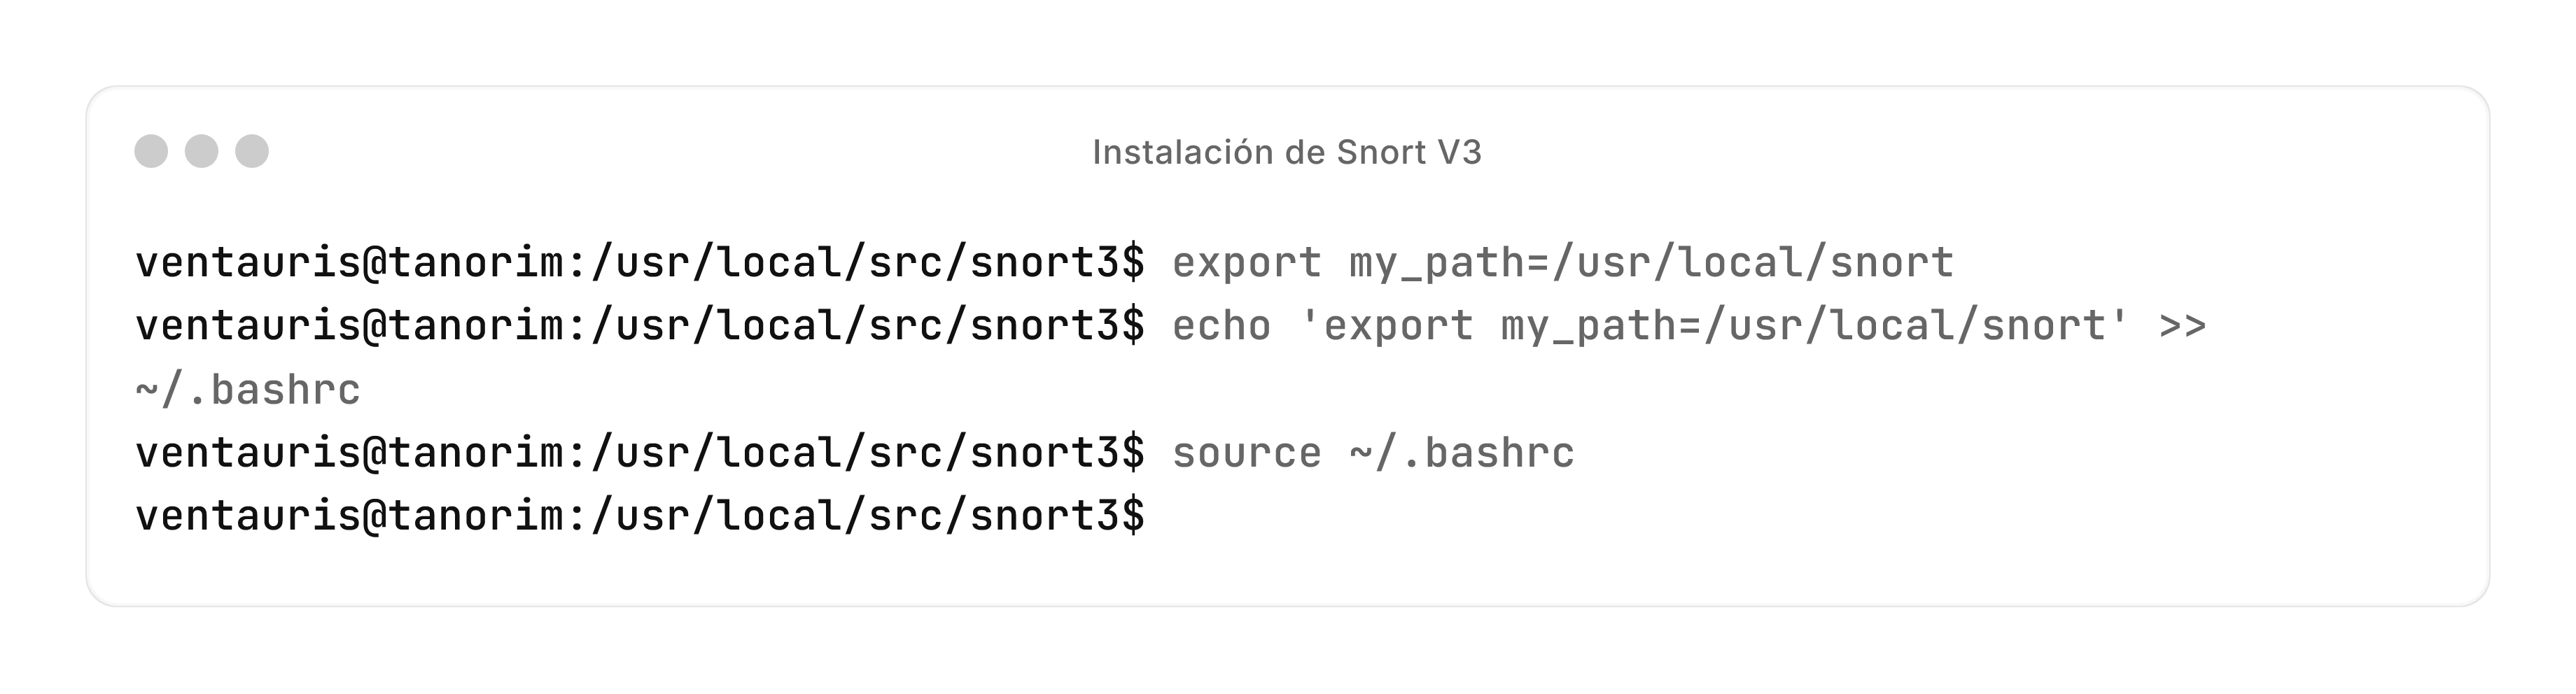
\includegraphics[scale=0.12]{instalacion_snort/18-18.png}
	\caption{Definiendo la ruta de instalación de Snort.}
\end{figure}

\newpage

Ejecutamos el script \texttt{configure\_cmake.sh} para configurar la compilación de \textbf{Snort 3}. Se especifica el prefijo de instalación con \texttt{\$my\_path}. Se generan los archivos de configuración y se definen las opciones de características, incluyendo los módulos \texttt{DAQ} que se activarán.

\begin{figure}[H]
	\centering
	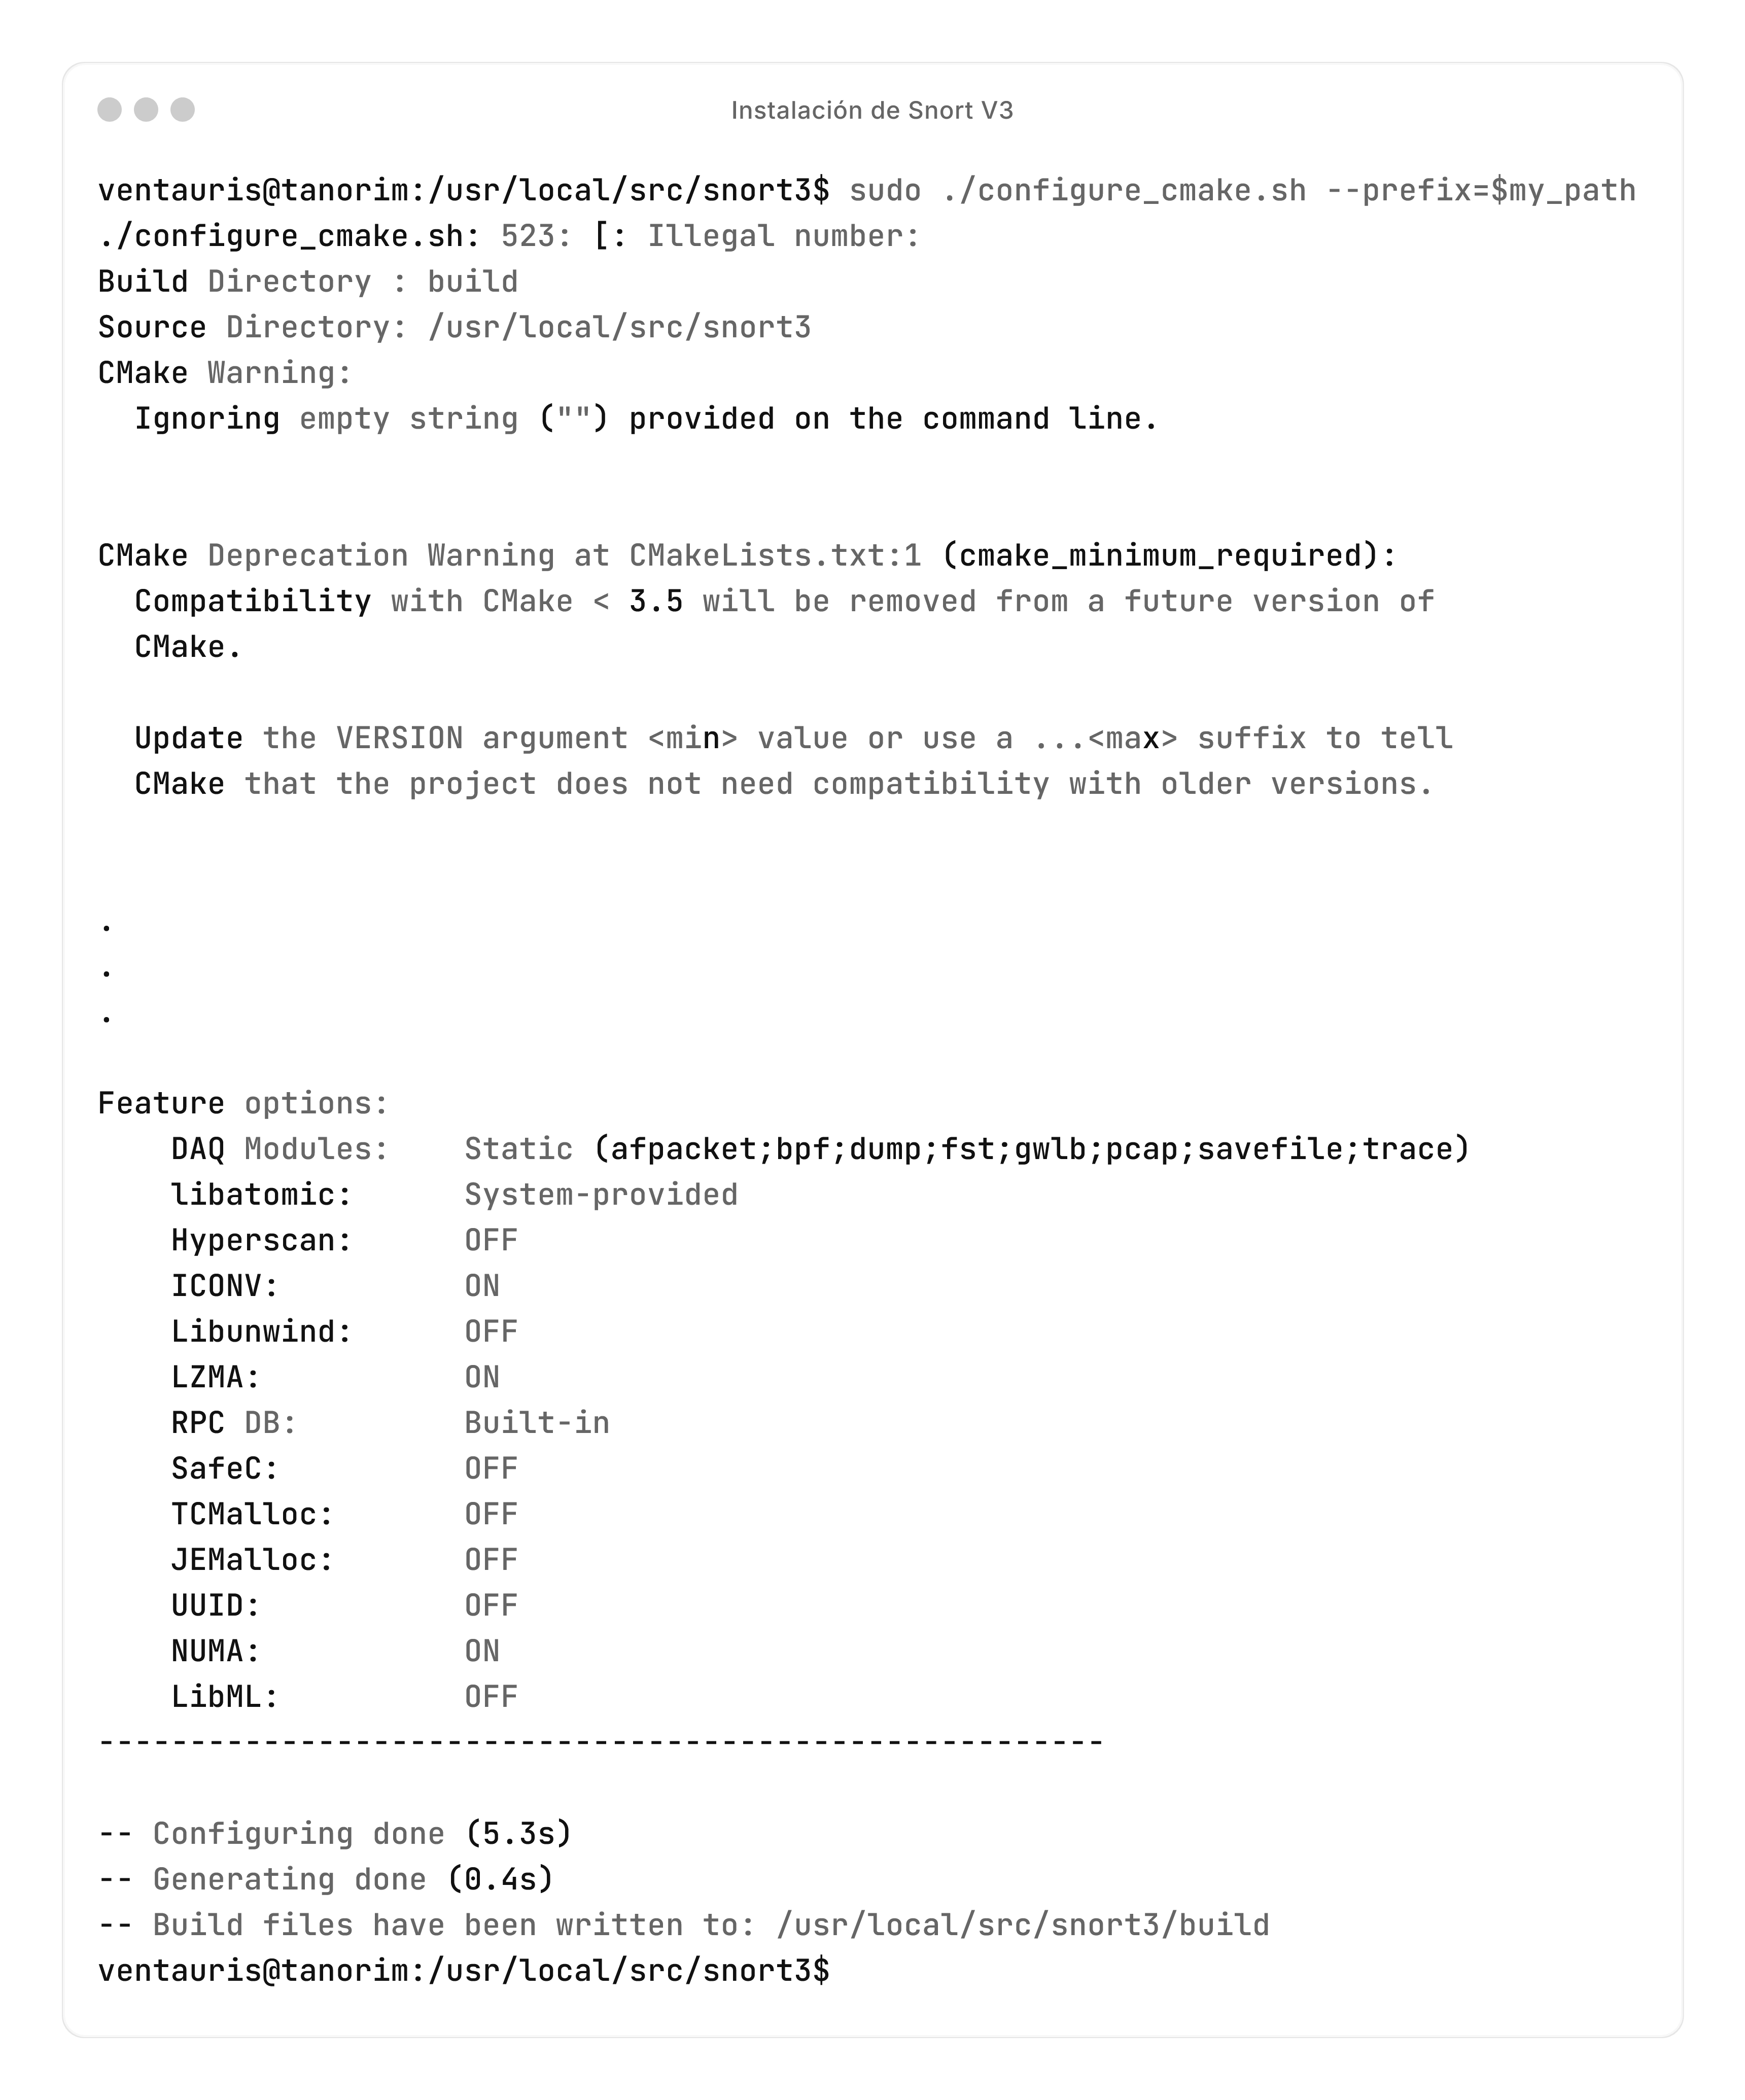
\includegraphics[scale=0.12]{instalacion_snort/21-21.png}
	\caption{Configurando Snort 3 con \texttt{CMake}.}
\end{figure}

\newpage

\subsubsection*{Compilación e instalación de Snort}

Compilamos \textbf{Snort} con \texttt{make -j \$(nproc)}, lo que nos permite aprovechar todos los núcleos del procesador para acelerar el proceso.

\begin{figure}[H]
	\centering
	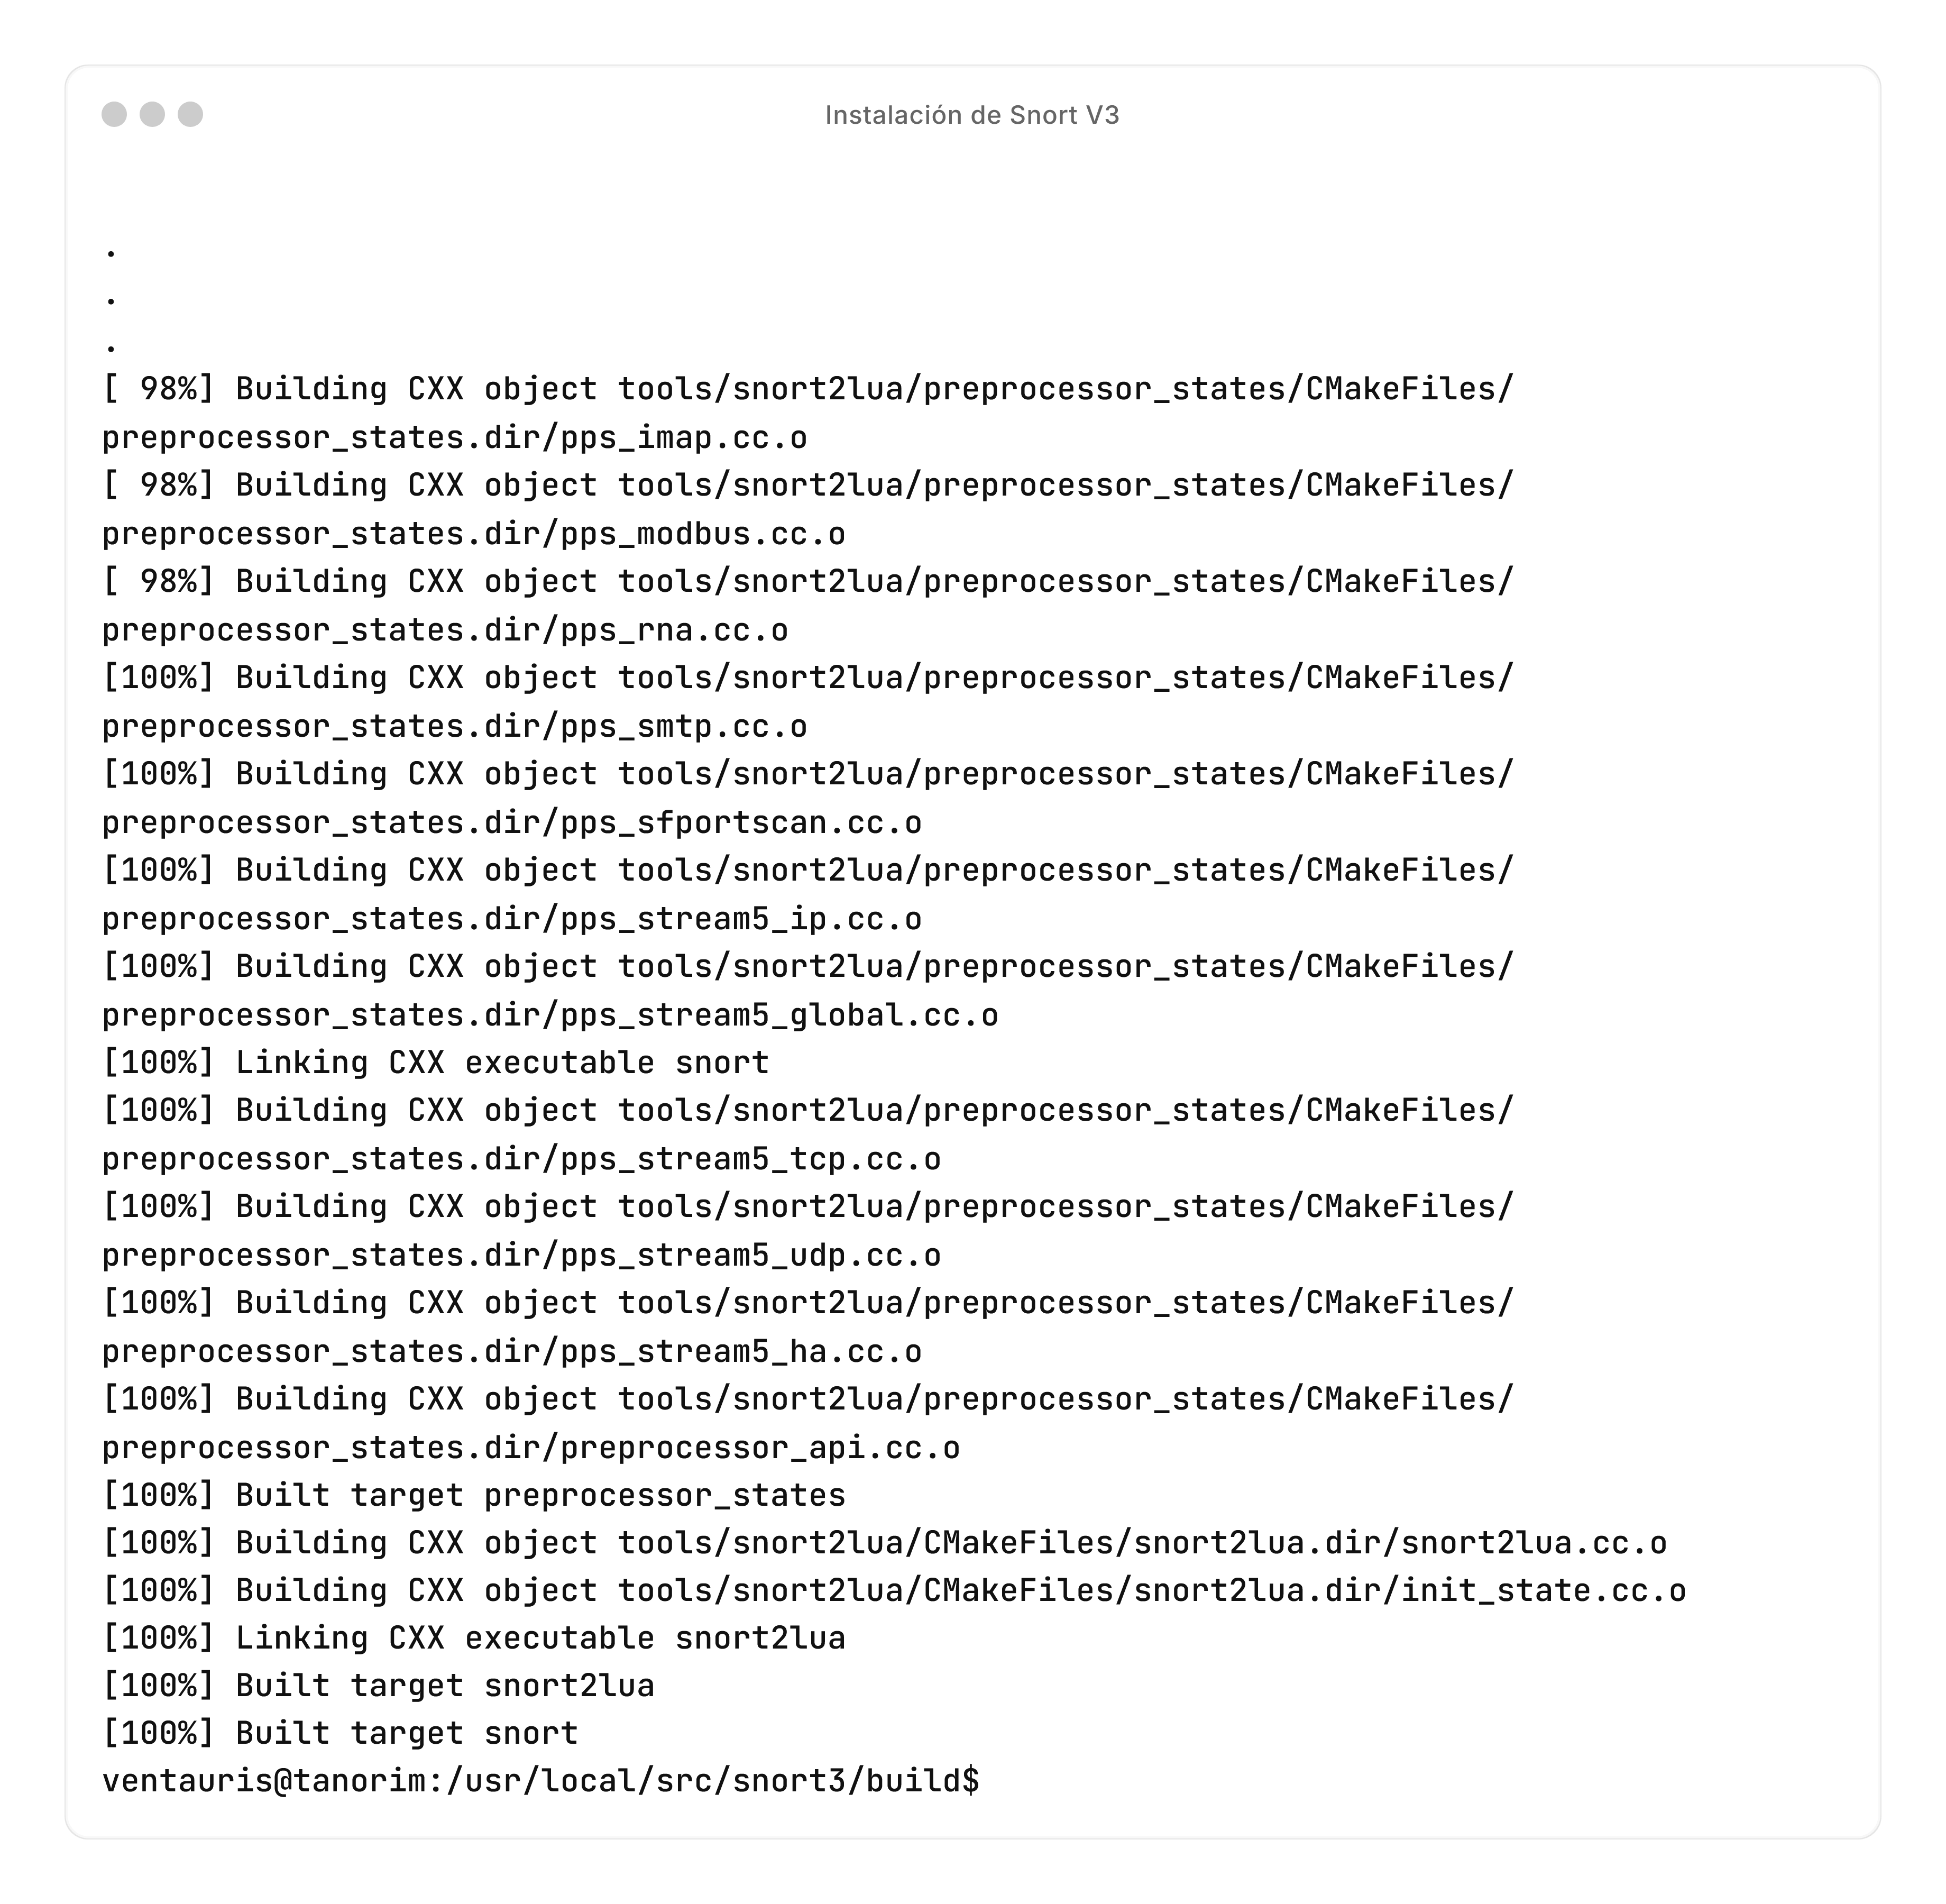
\includegraphics[scale=0.12]{instalacion_snort/22-22.png}
	\caption{Compilación de Snort.}
\end{figure}

\newpage

Instalamos Snort tras haberlo compilado con \texttt{sudo make install}. Este comando copia los archivos generados en sus respectivas ubicaciones dentro del sistema.

\begin{figure}[H]
	\centering
	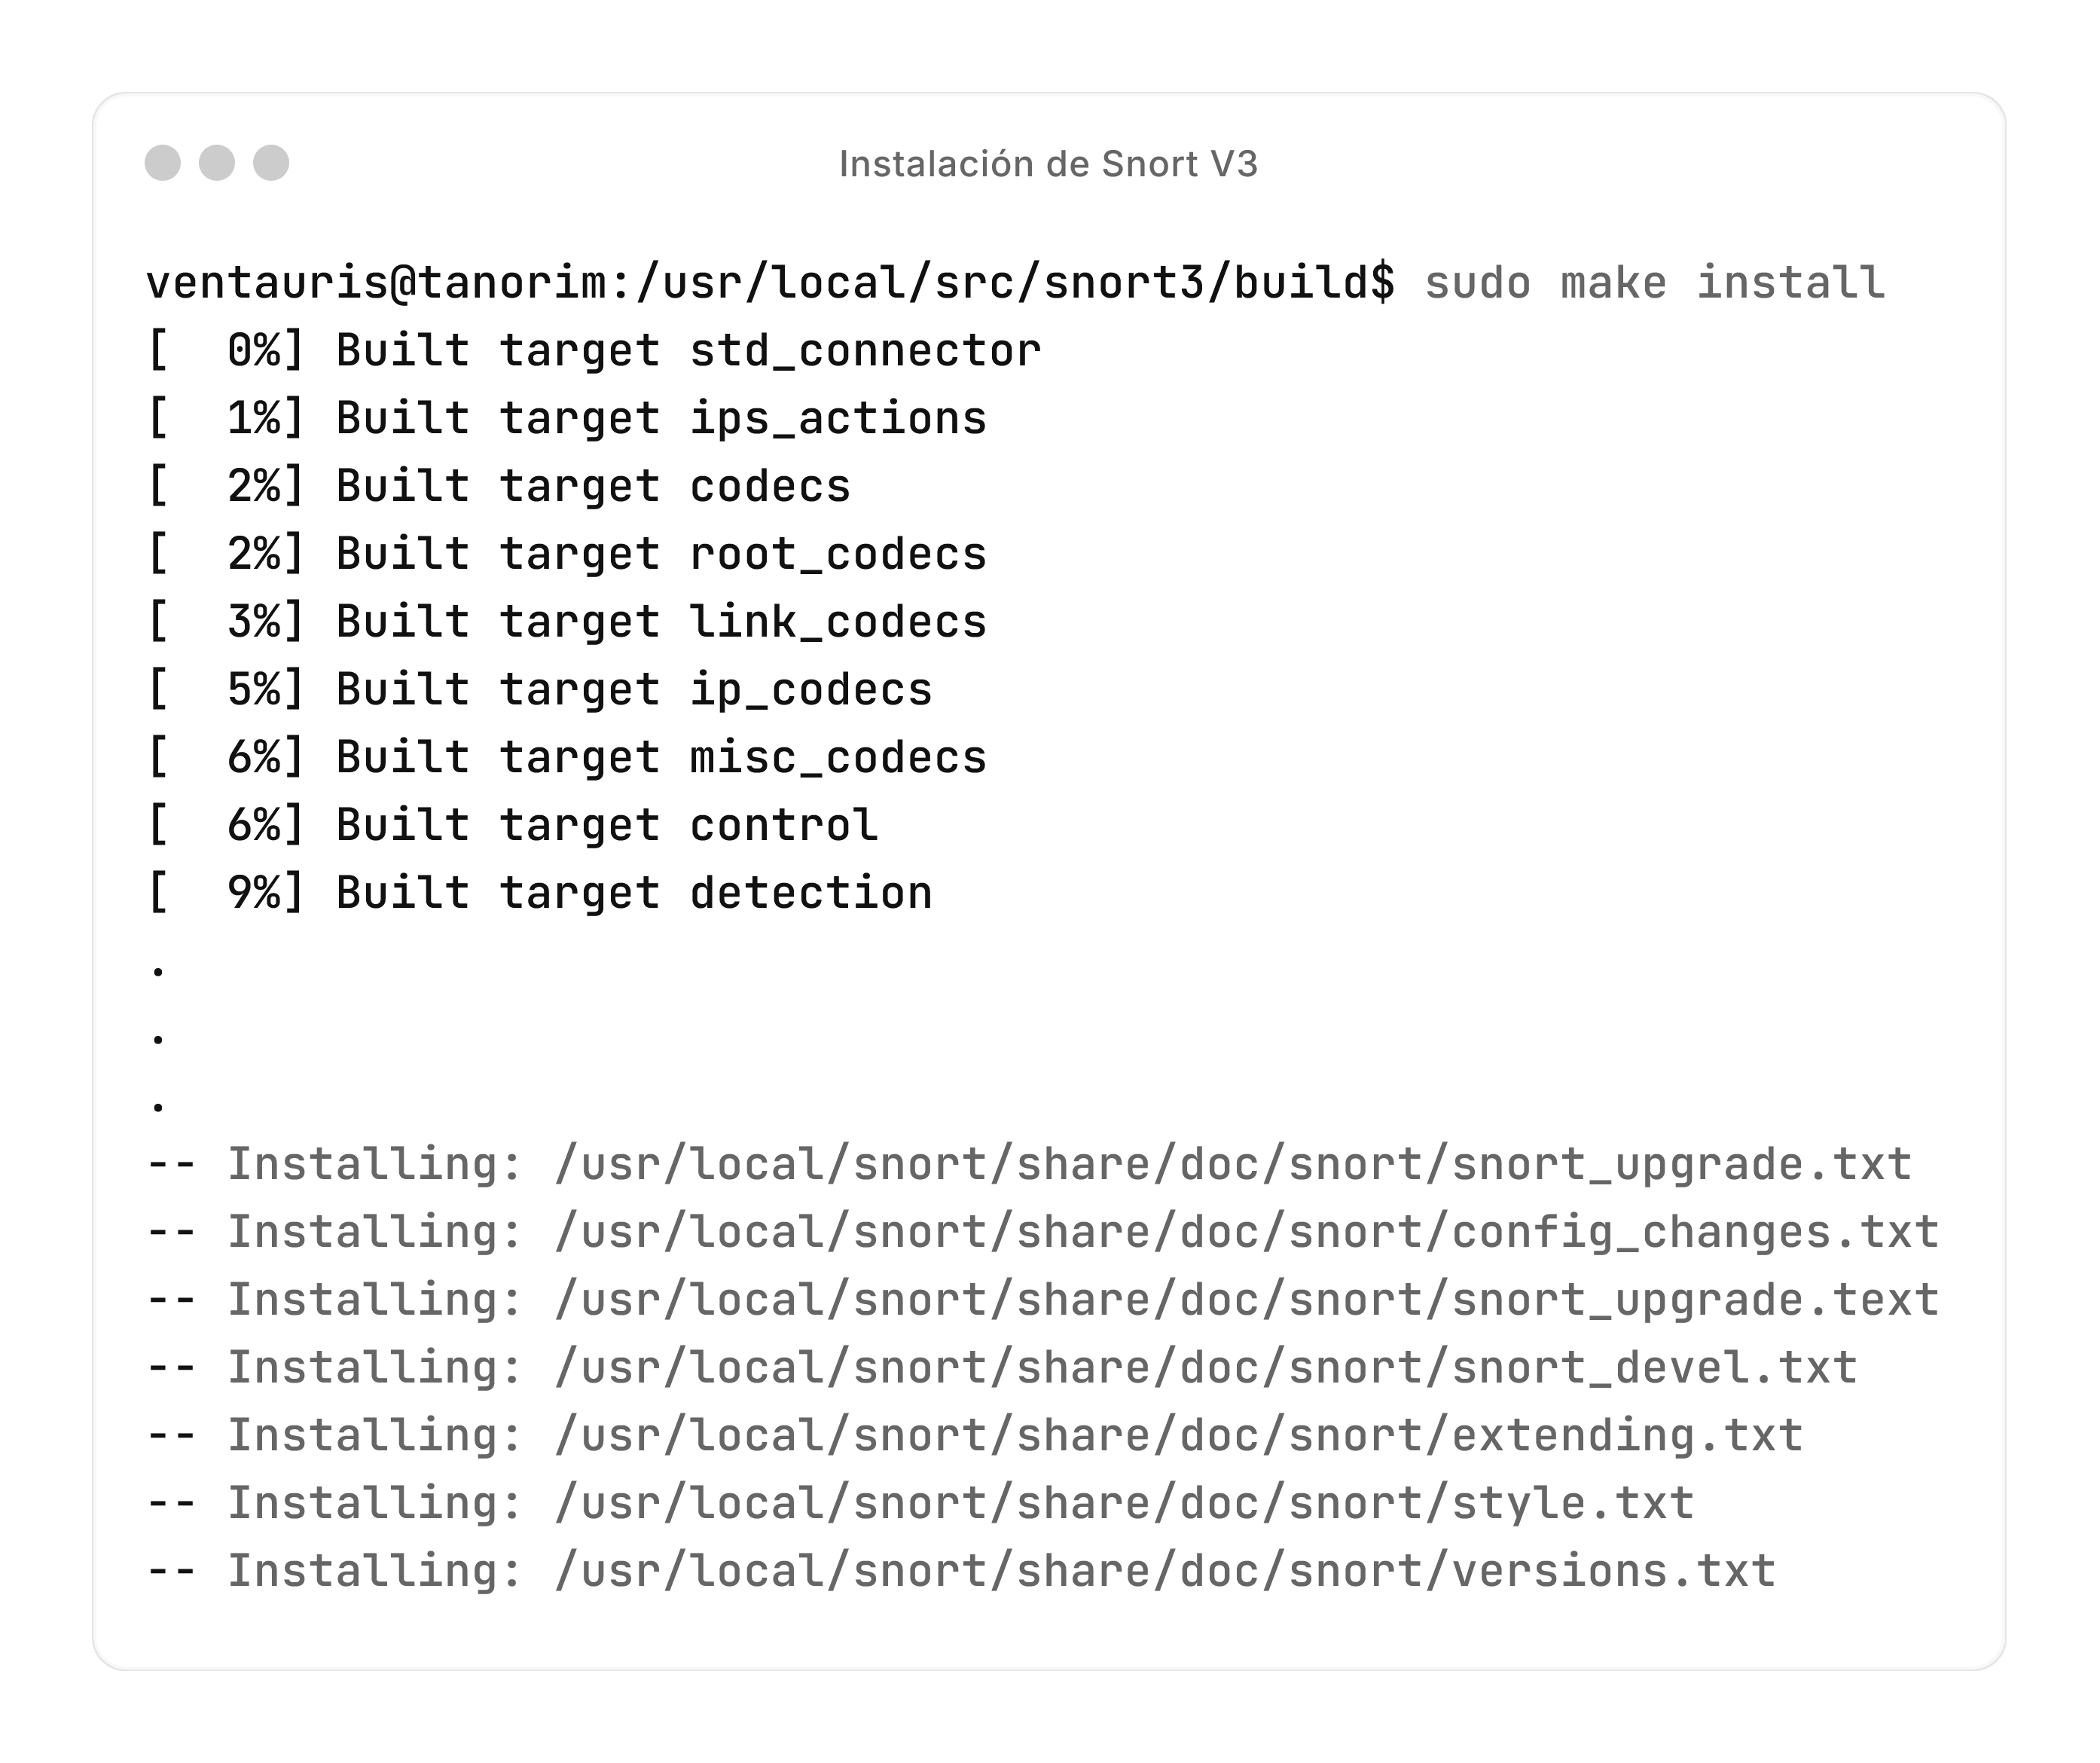
\includegraphics[scale=0.12]{instalacion_snort/23-23.png}
	\caption{Instalación de Snort.}
\end{figure}

\subsubsection*{Configuración inicial y validación}

Finalmente, verificamos que \textbf{Snort} se ha instalado correctamente con el comando: \\
\texttt{/usr/local/snort/bin/snort -V}. Esto nos muestra la versión instalada (\textbf{3.7.1.0}) junto con las bibliotecas y dependencias utilizadas, como \texttt{DAQ}, \texttt{libpcap}, \texttt{LuaJIT}, \texttt{OpenSSL}, entre otras.

\begin{figure}[H]
	\centering
	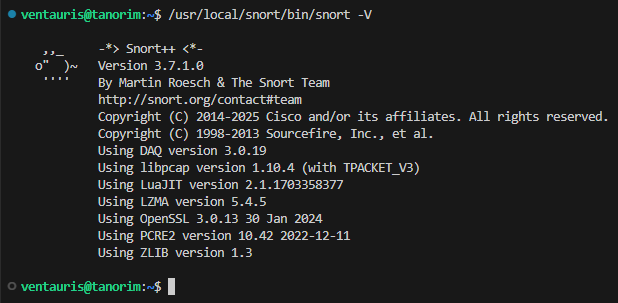
\includegraphics[scale=0.7]{instalacion_snort/24.png}
	\caption{Snort instalado con éxito.}
\end{figure}

\newpage

Creamos el directorio de configuración de Snort (\texttt{/usr/local/snort/etc/snort}) y copiamos los archivos de configuración en formato \texttt{Lua} desde el directorio fuente de \textbf{Snort 3}. Luego, ejecutamos Snort con la configuración especificada para validar que todo esté correctamente configurado. La salida muestra que Snort ha cargado las reglas y módulos sin errores ni advertencias.

\begin{figure}[H]
	\centering
	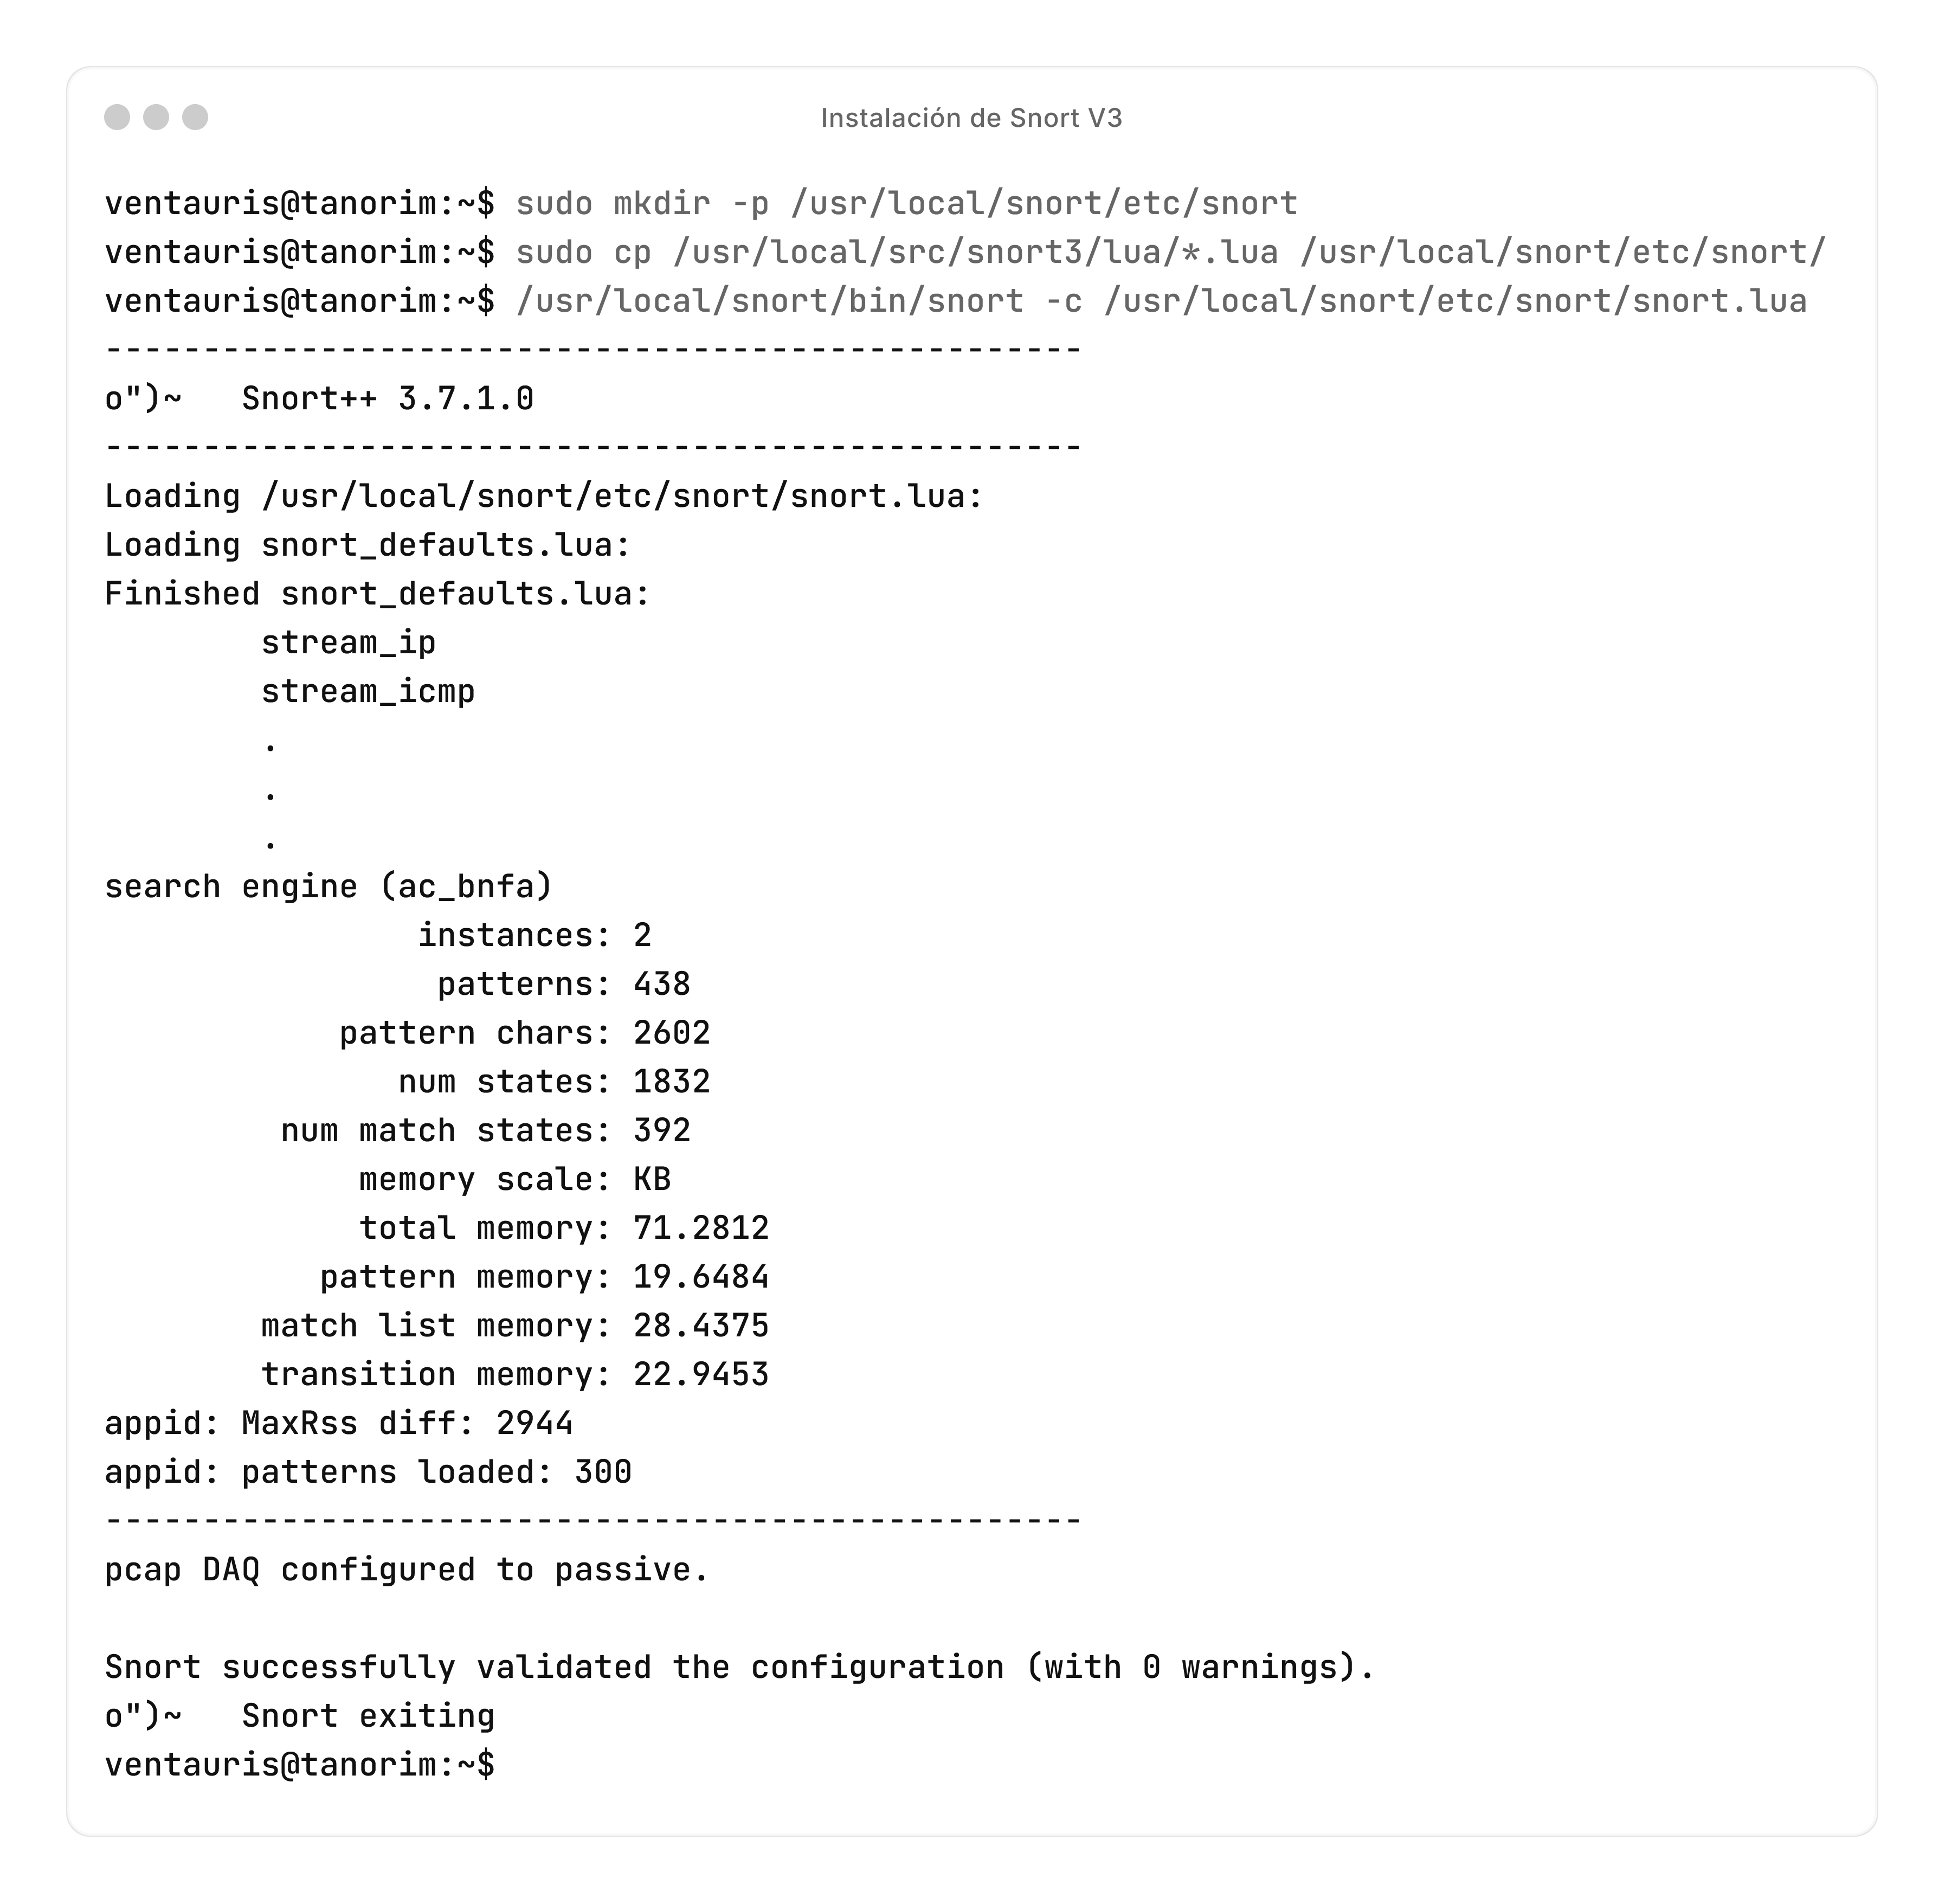
\includegraphics[scale=0.12]{instalacion_snort/25-25.png}
	\caption{Configuración de Snort validada con éxito.}
\end{figure}

\newpage

\subsection{Instalación de reglas y plugins}

Tras la correcta instalación de \textbf{Snort}, aprovecharemos la arquitectura modular introducida en la versión 3, la cual utiliza archivos con extensión \texttt{.lua} para gestionar su configuración de forma más flexible y estructurada. A continuación, se presenta una guía paso a paso sobre cómo instalar las reglas básicas proporcionadas por la comunidad de Snort, conocidas como \textit{Community Rules}.

Descargamos las \textit{Community Rules} de Snort utilizando el comando \texttt{wget}, seguido de su descompresión mediante \texttt{tar}. Estas reglas constituyen un conjunto de firmas predefinidas para detectar amenazas comunes en entornos de red.

\begin{figure}[H]
	\centering
	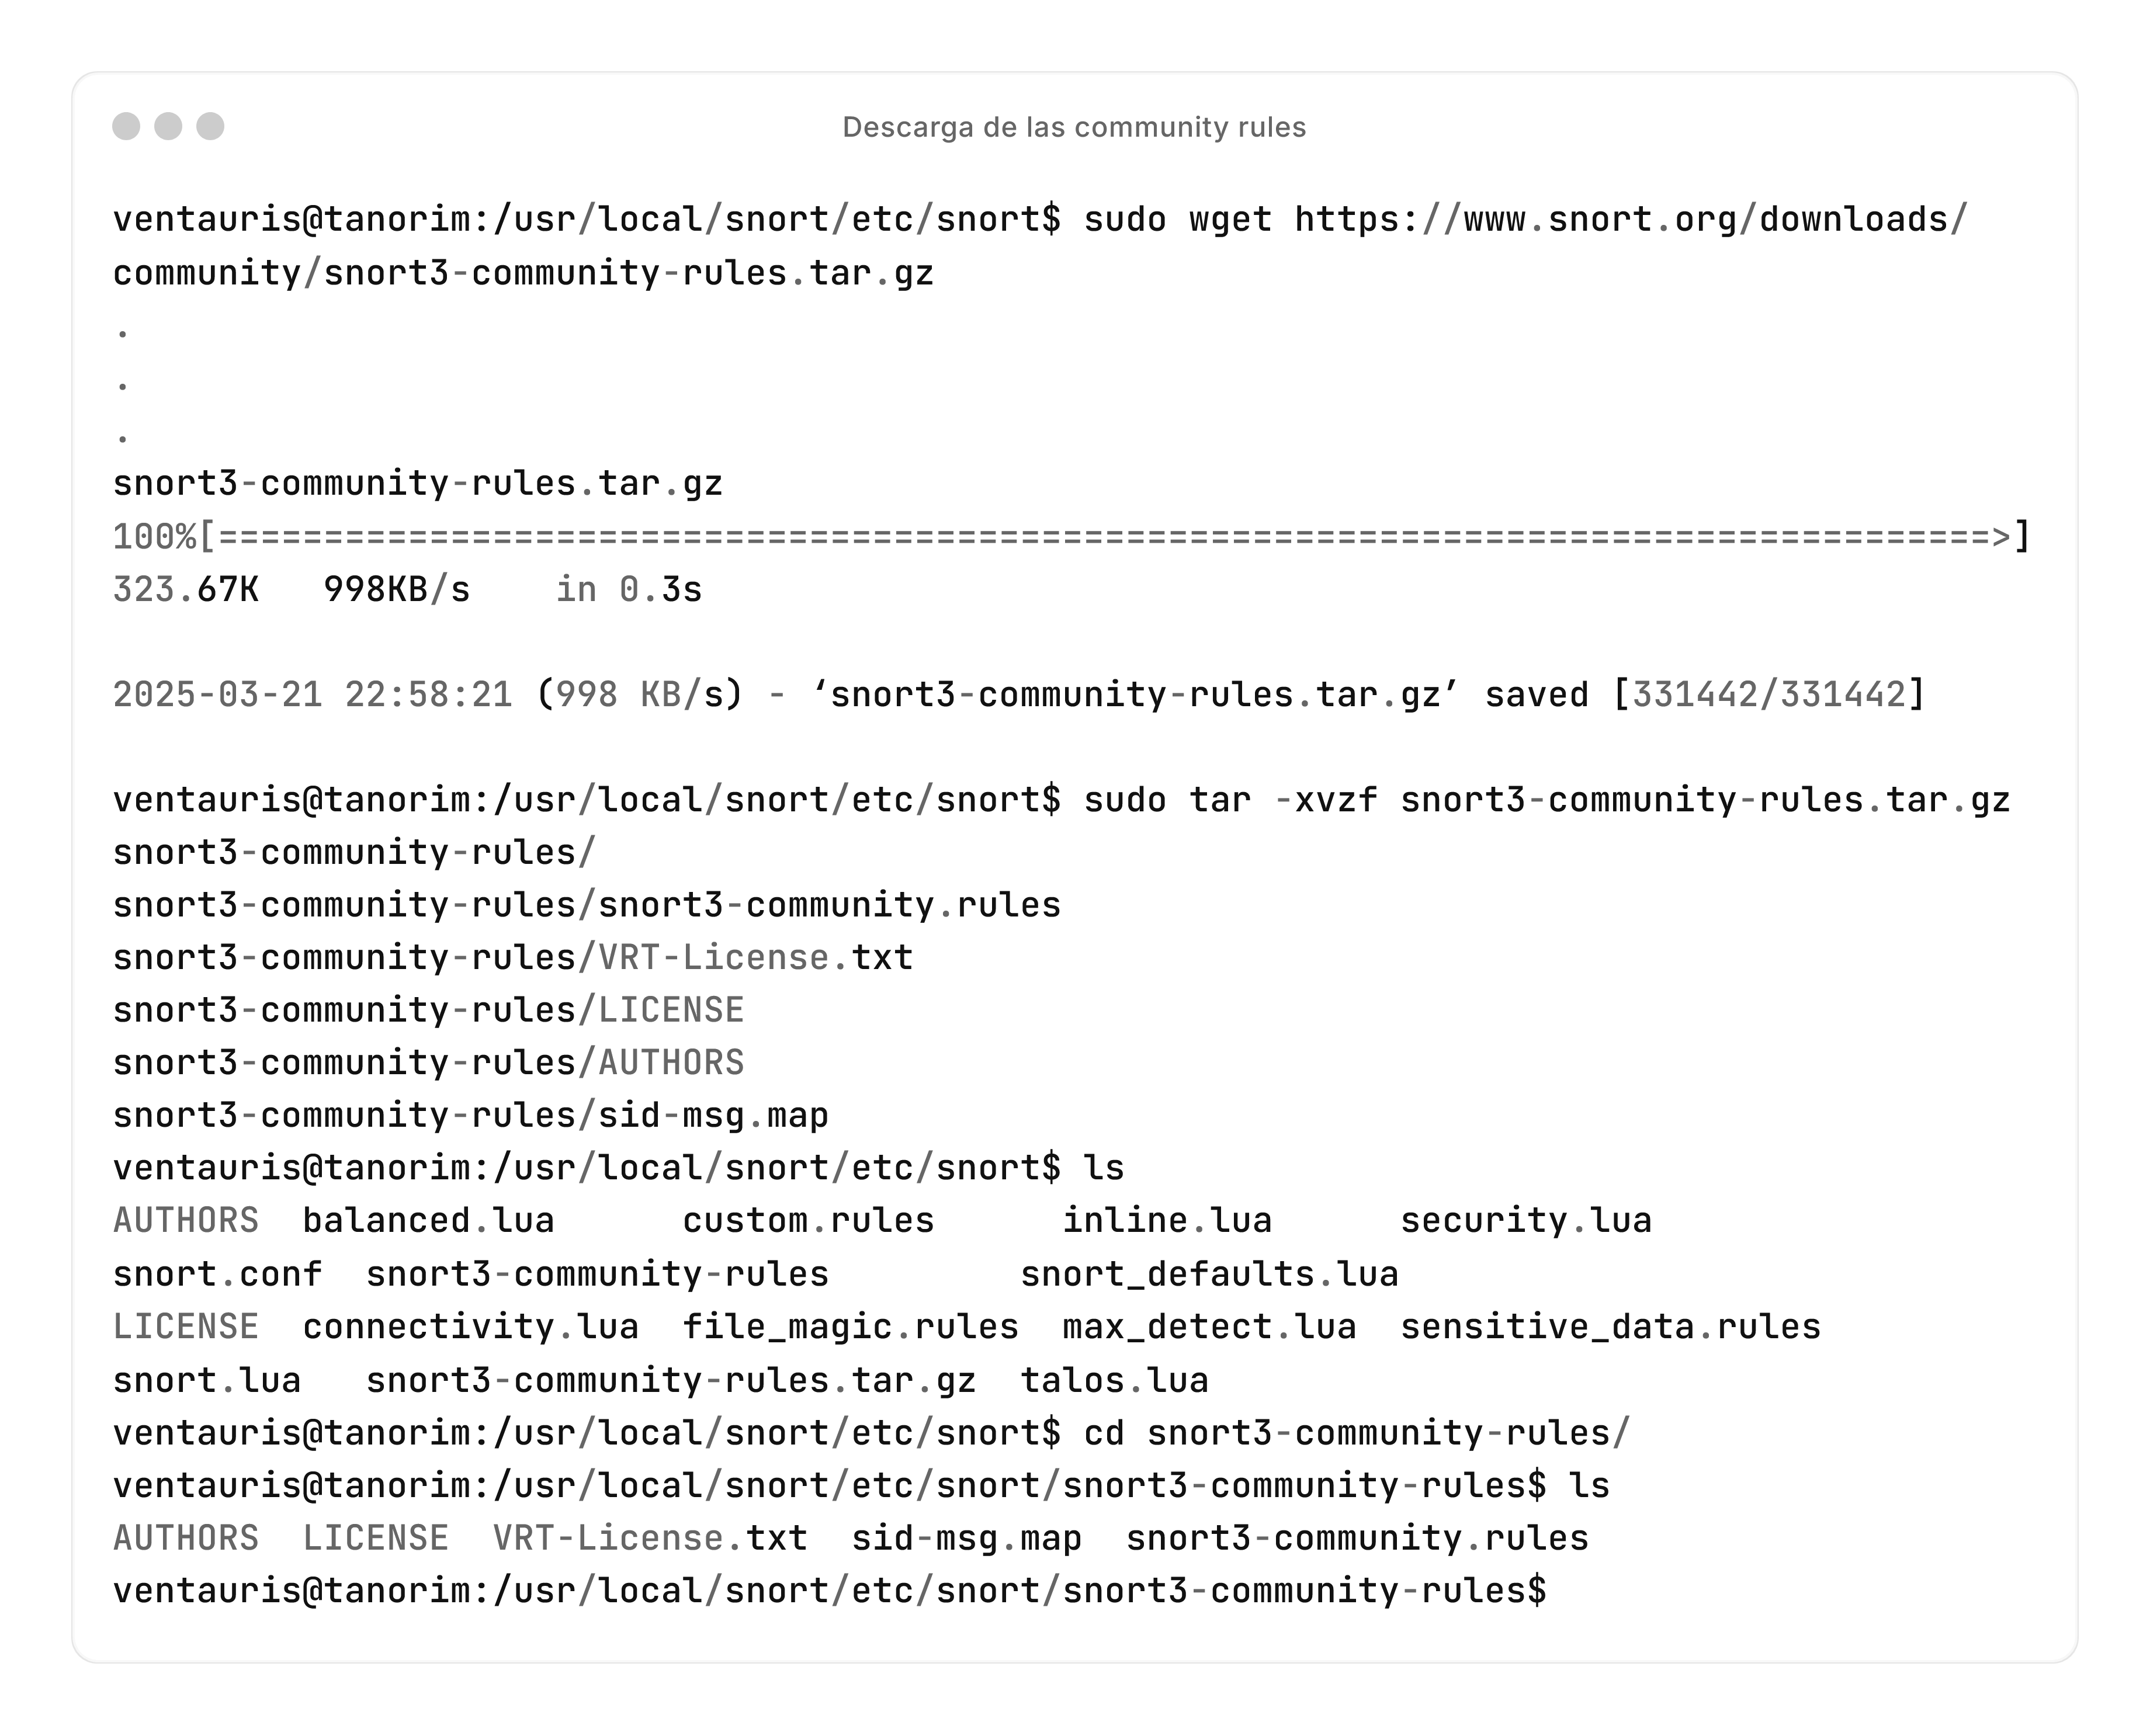
\includegraphics[scale=0.12]{instalacion_reglas_snort/1-1.png}
	\caption{Añadiendo reglas preconfiguradas a Snort.}
\end{figure}

\pagebreak

Posteriormente, editamos el archivo \texttt{snort.lua} \cite{snort_user_manual}, ubicado en \path{/usr/local/snort/etc/snort/}, para incluir la ruta del archivo \texttt{community.rules}. Esto permite que Snort cargue automáticamente estas reglas al iniciar y pueda utilizarlas para detectar patrones maliciosos en el tráfico de red. La edición del archivo puede realizarse con herramientas como \texttt{nano}, \texttt{vim} o cualquier otro editor de texto de preferencia.

\begin{figure}[H]
	\centering
	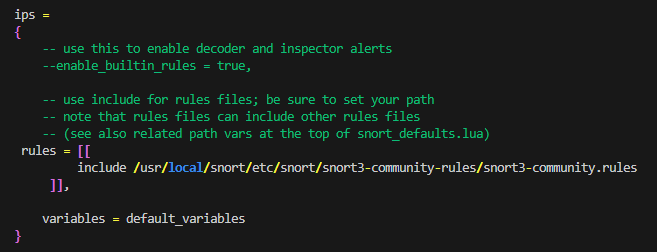
\includegraphics[scale=0.8]{instalacion_reglas_snort/2.png}
	\caption{Modificación de \texttt{snort.lua} para agregar las reglas preconfiguradas.}
\end{figure}

Una vez agregadas las reglas a \texttt{snort.lua}, realizamos una validación de la configuración ejecutando Snort en modo prueba. Esto permite comprobar que no existan errores sintácticos o de carga, garantizando así que el sistema pueda funcionar correctamente.

\begin{figure}[H]
	\centering
	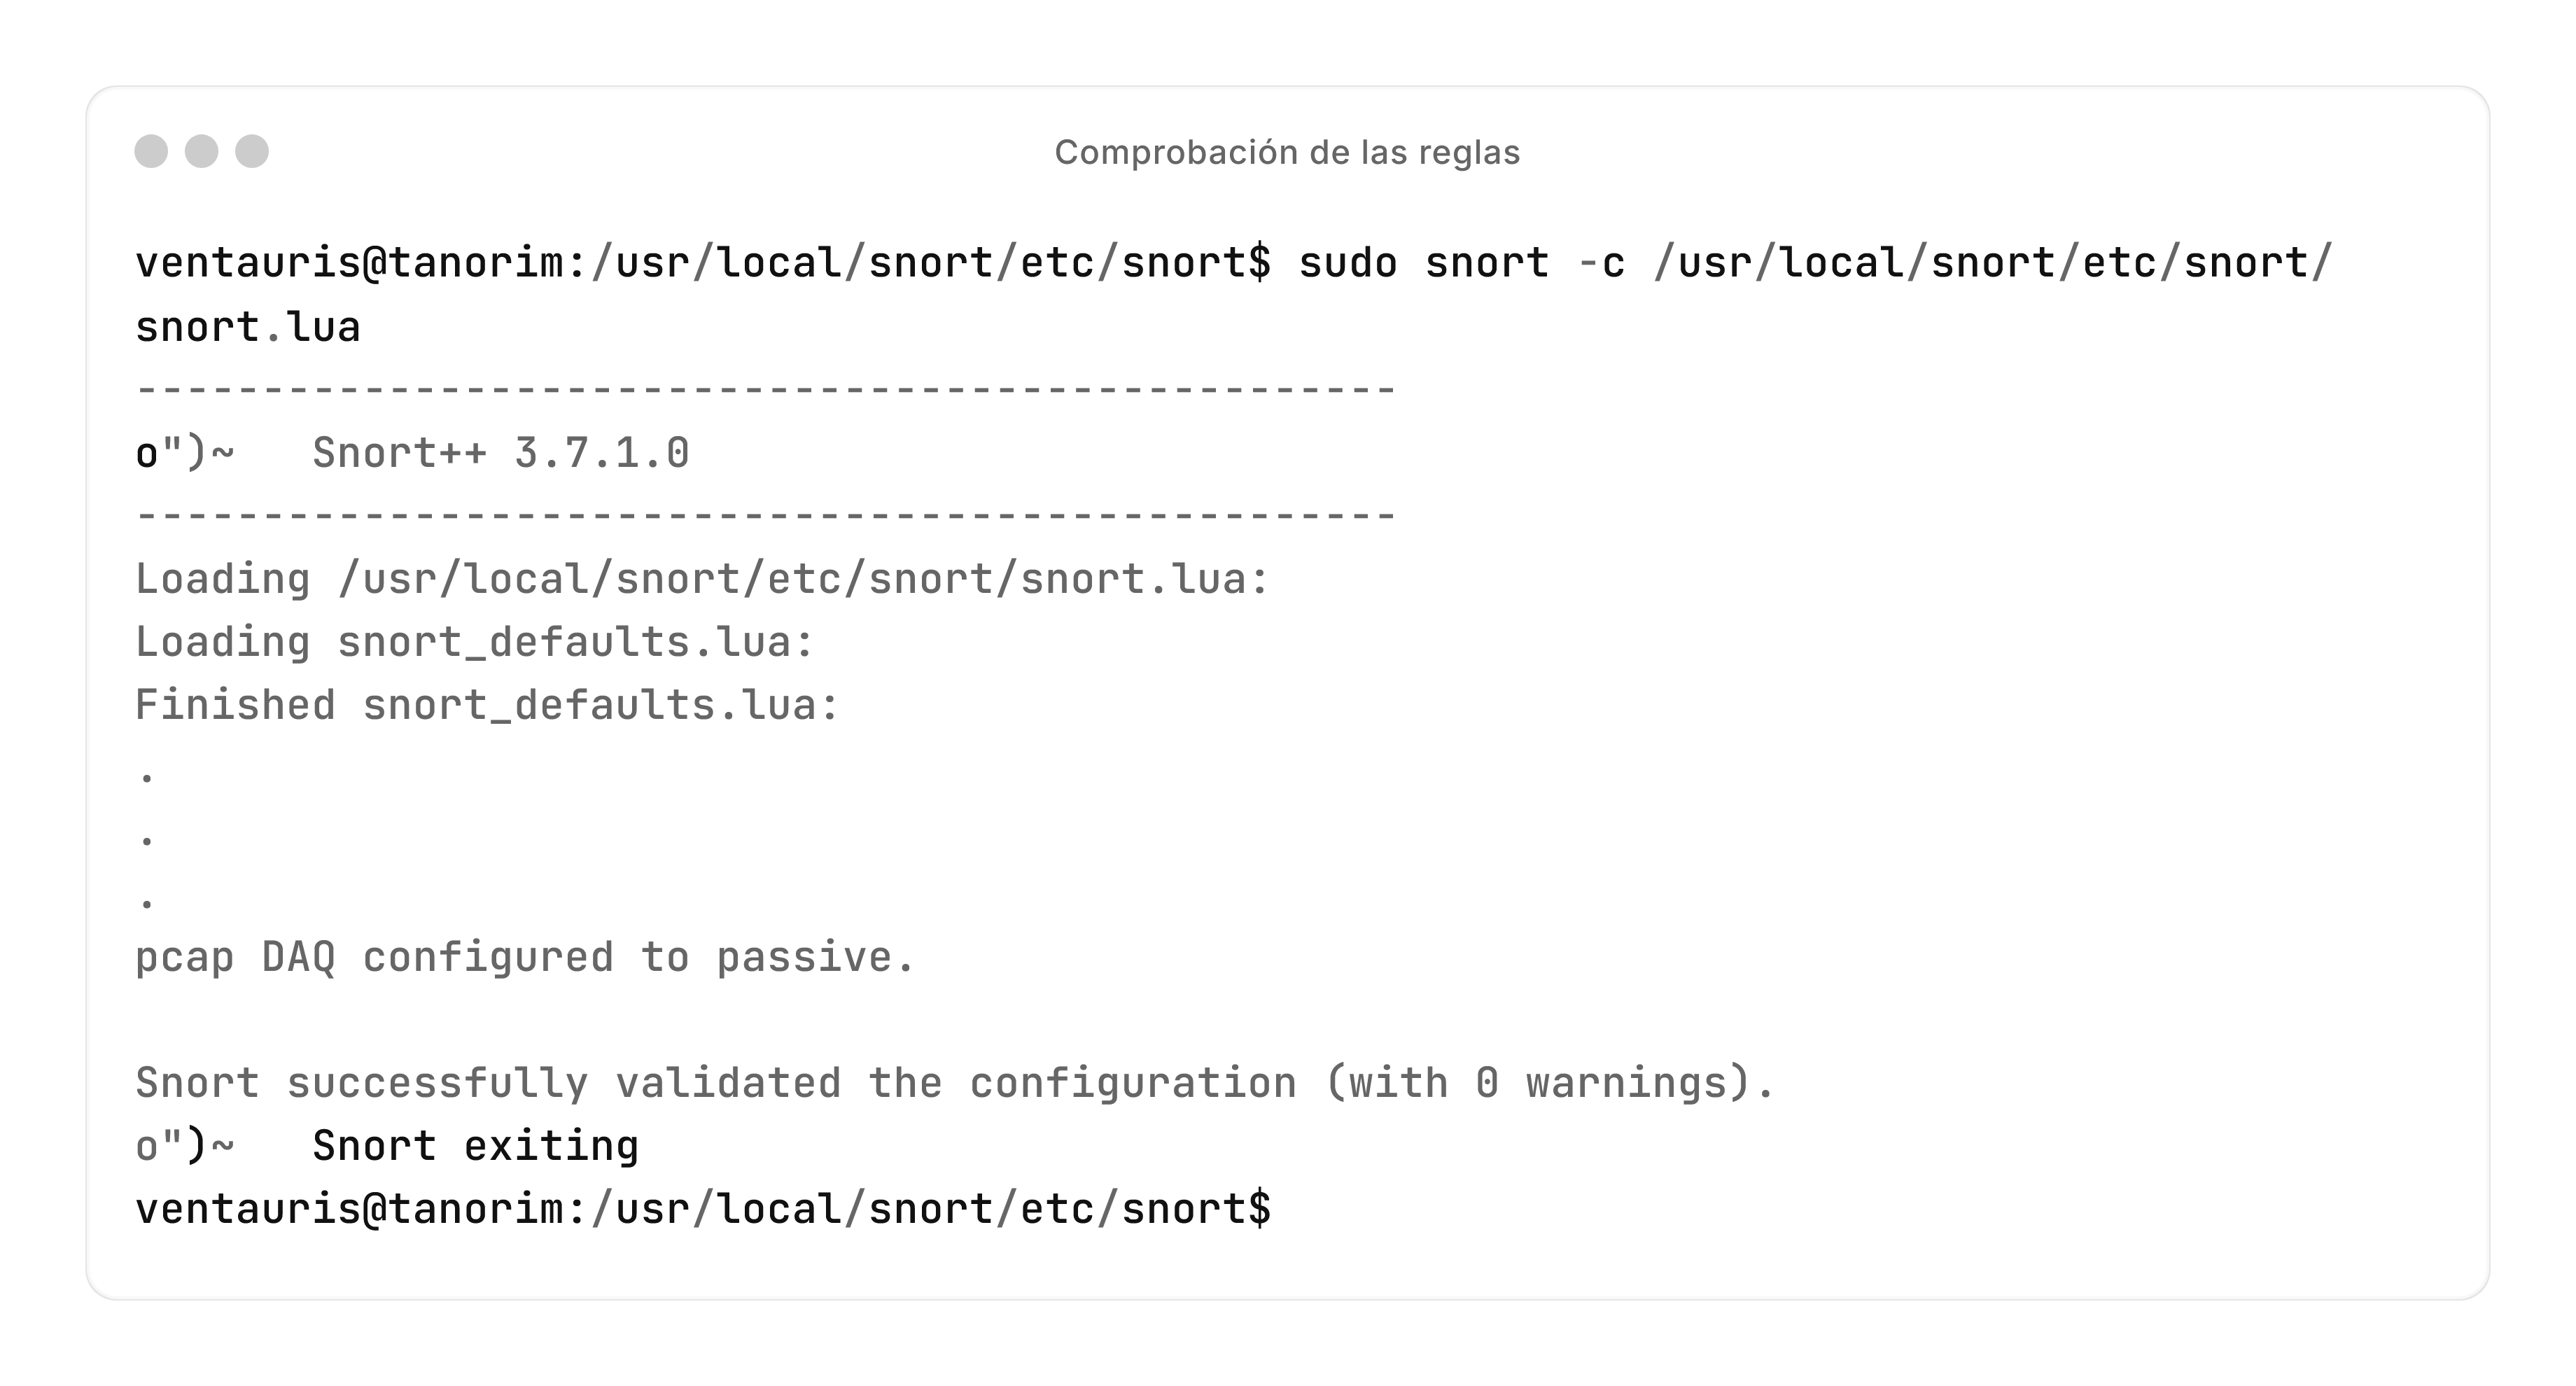
\includegraphics[scale=0.12]{instalacion_reglas_snort/3-3.png}
	\caption{Validación configuración de Snort.}
\end{figure}

\newpage

\subsubsection*{Configuración preprocesador HTTP Inspect}

Accedemos al archivo \texttt{snort.lua} y localizamos la sección correspondiente al preprocesador \texttt{http\_inspect = \{\}}. En ella escribimos los parámetros adecuados para la gestión y protección de una red corporativa de pequeña o mediana empresa (PYME). Esta configuración permite a Snort analizar a fondo el tráfico HTTP y detectar comportamientos anómalos asociados a amenazas comunes como ataques por inyección, carga de malware o manipulación de cabeceras.

Las reglas aplicadas son las siguientes:
\newline

\begin{table}[ht]
	\centering
	\begin{tabular}{l l p{7cm}}
		\hline
		\textbf{Parámetro} & \textbf{Valor} & \textbf{Uso en una PYME}\\
		\hline
		\texttt{request\_depth}       & \texttt{-1} & Inspeccionar todo el contenido de la petición HTTP. Permite detectar inyecciones SQL, código malicioso y malware embebido.\\
		\texttt{response\_depth}      & \texttt{-1} & Revisar la totalidad de la respuesta enviada por el servidor, útil para detectar descargas de archivos maliciosos.\\
		\texttt{unzip}                & \texttt{true} & Habilita la descompresión de contenidos codificados como gzip o deflate. Evita que el contenido malicioso comprimido pase desapercibido.\\
		\texttt{oversize\_dir\_length}& \texttt{500} & Genera alertas si una URI presenta una ruta anormalmente larga, característica común en ataques de desbordamiento o evasión.\\
		\texttt{maximum\_headers}     & \texttt{200} & Detecta un número excesivo de cabeceras HTTP, que puede ser indicio de ataques por manipulación de protocolo.\\
		\hline
	\end{tabular}
	\caption{Parámetros de \texttt{http\_inspect}.}
\end{table}

\begin{figure}[H]
	\centering
	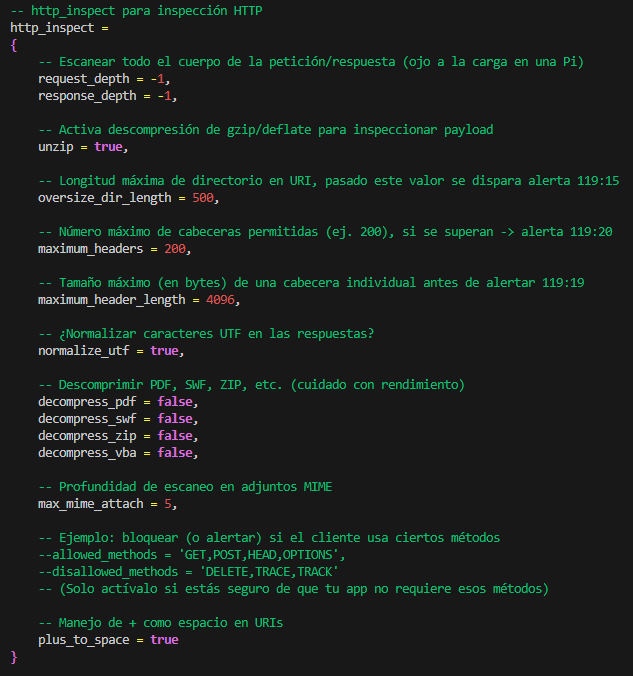
\includegraphics[scale=0.5]{http_inspect/4.png}
	\caption{Configuración \texttt{http\_inspect}.}
\end{figure}

\begin{figure}[H]
	\centering
	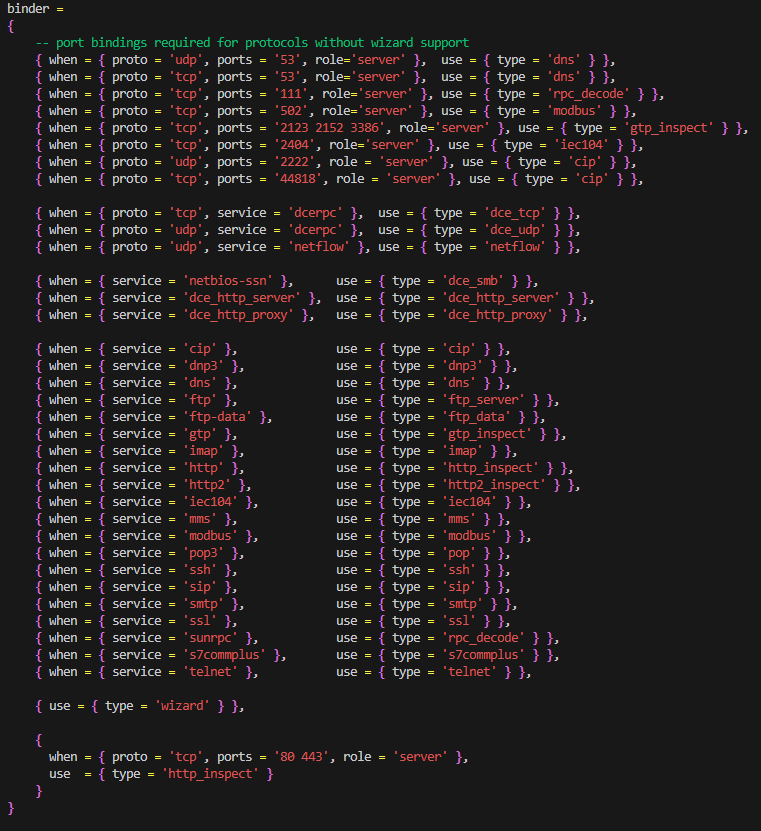
\includegraphics[scale=0.45]{http_inspect/5.png}
	\caption{Configuración de \texttt{binders}.}
\end{figure}


%%%%%%%%%%%%%%%%%%HECHO4

Además de la configuración general de \texttt{http\_inspect} mostrada en la Figura 6.30, es necesario agregar, al final de la sección de \texttt{binders} en el archivo \texttt{snort.lua}, el bloque de código representado en la Figura 6.31 para asegurar su correcto funcionamiento.
\newline

Esta configuración adicional es esencial para que \textbf{Snort} pueda vincular correctamente el tráfico HTTP con su correspondiente módulo de inspección durante el análisis en tiempo real. Sin este paso, es posible que el motor de detección no aplique correctamente las reglas diseñadas para HTTP, reduciendo así la eficacia del sistema de detección de intrusiones.
\newline

Por último, validamos la configuración ejecutando Snort en modo prueba para asegurarnos de que no se han introducido errores y que todas las configuraciones han sido cargadas exitosamente.

\begin{figure}[H]
	\centering
	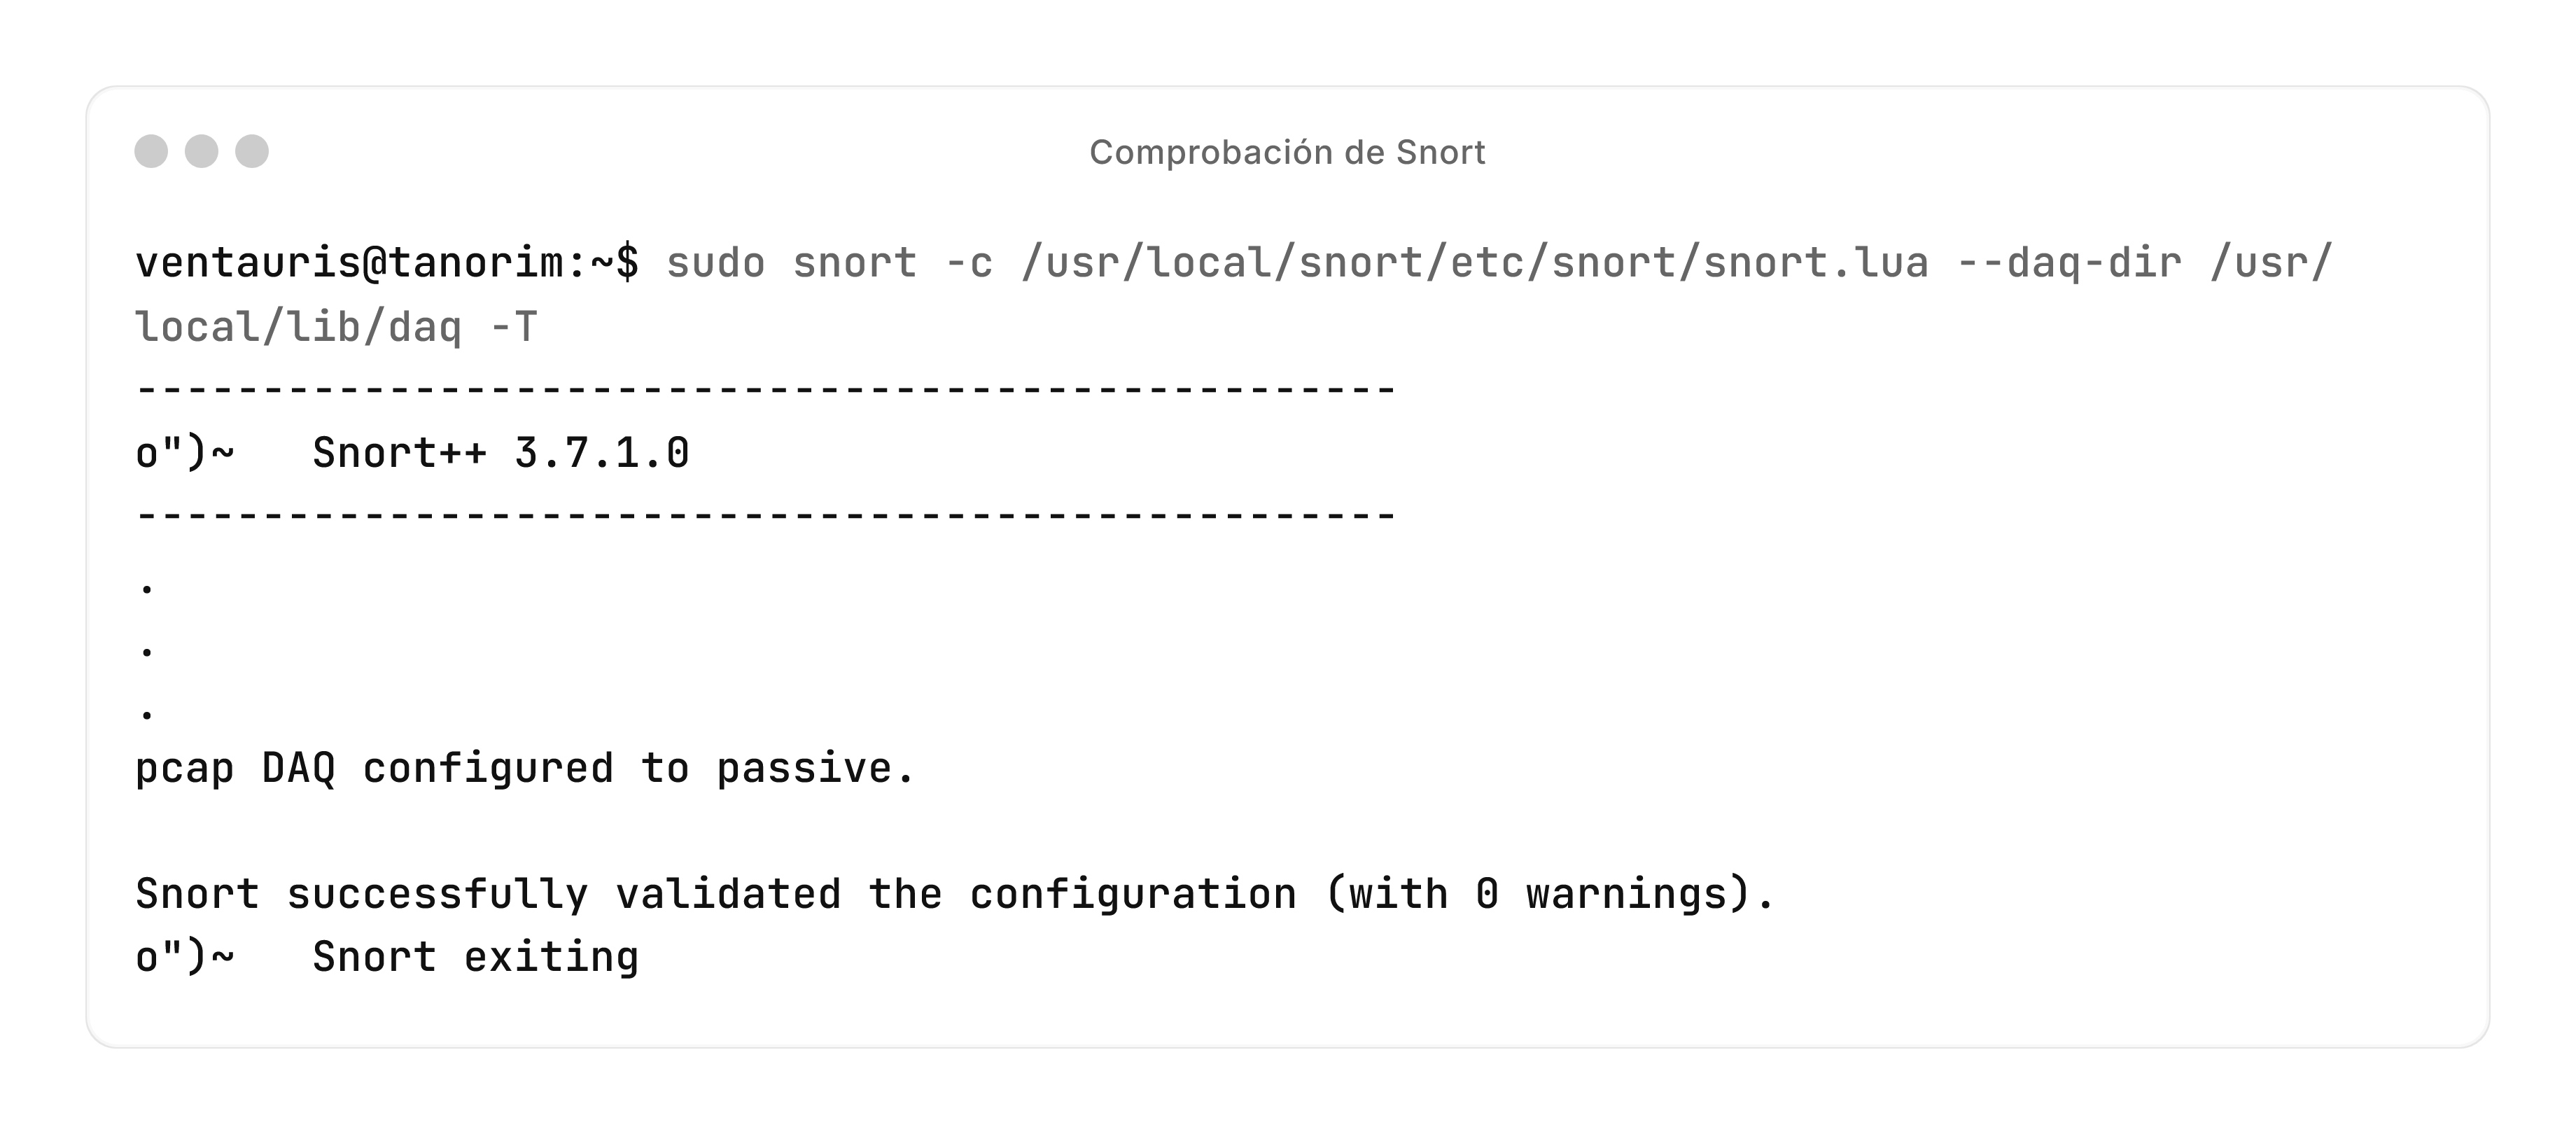
\includegraphics[scale=0.1]{http_inspect/6-6.png}
	\caption{Validación de la configuración.}
\end{figure}


\subsubsection*{SSL Inspector}

El siguiente módulo que habilitaremos será el \textbf{SSL Inspector}. El procedimiento de activación es similar al seguido en módulos anteriores. Comenzaremos por modificar el archivo \texttt{snort.lua}, donde localizaremos la sección correspondiente a \texttt{ssl} y añadiremos el bloque de configuración mostrado a continuación.

\begin{figure}[H]
	\centering
	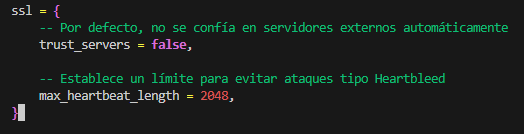
\includegraphics[scale=0.8]{ssl_inspect/8.png}
	\caption{Configuración de SSL.}
\end{figure}

Posteriormente, es necesario vincular la configuración de \texttt{ssl} en la sección \texttt{binders}, en caso de que no se haya hecho previamente. Esta vinculación garantiza que el tráfico cifrado sea correctamente dirigido al módulo de inspección SSL.

\begin{figure}[H]
	\centering
	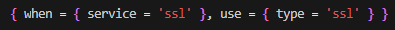
\includegraphics[scale=0.8]{ssl_inspect/9.png}
	\caption{Vincular con \texttt{binders}.}
\end{figure}

A continuación, verificamos la configuración de Snort para asegurarnos de que la sintaxis sea válida. Si todo es correcto, reiniciamos el servicio mediante \texttt{systemctl} para aplicar los cambios.

\newpage

\begin{lstlisting}[language=bash, label={lst:validacion_snort}]
	# Validar la configuracion de Snort
	sudo snort -c /usr/local/snort/etc/snort/snort.lua -T
	
	# Reiniciar el servicio de Snort
	sudo systemctl restart snort
\end{lstlisting}


\subsubsection*{Stream IP}

Antiguamente conocido como \texttt{Frag3}, este preprocesador ha sido reemplazado por una versión más moderna bajo el nombre de \textbf{Stream IP}. Este módulo es responsable de reensamblar fragmentos de paquetes IP para prevenir técnicas de evasión. Su configuración se realiza en el archivo \texttt{snort.lua}.

\begin{figure}[H]
	\centering
	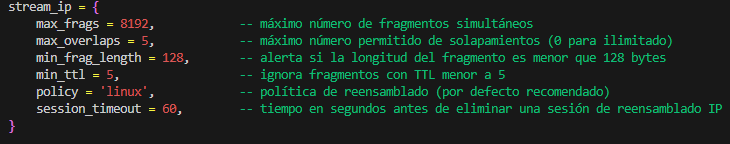
\includegraphics[scale=0.8]{stream_ip/1.png}
	\caption{Configuración de Stream IP.}
\end{figure}

Una vez completada la configuración, validamos la sintaxis del archivo y reiniciamos Snort para aplicar los cambios.

\newpage

\subsubsection*{Stream TCP}

Otro preprocesador que puede marcar la diferencia en protección de redes SOHO es \textbf{Stream TCP}, sucesor de \texttt{Stream5}. Este módulo permite el reensamblado de flujos TCP, lo cual es esencial para una inspección precisa del tráfico de red a nivel de sesión. Su configuración se realiza de forma similar a \texttt{Stream IP}. Tras editar \texttt{snort.lua}, comprobamos la validez de la sintaxis y reiniciamos el servicio.

\begin{figure}[H]
	\centering
	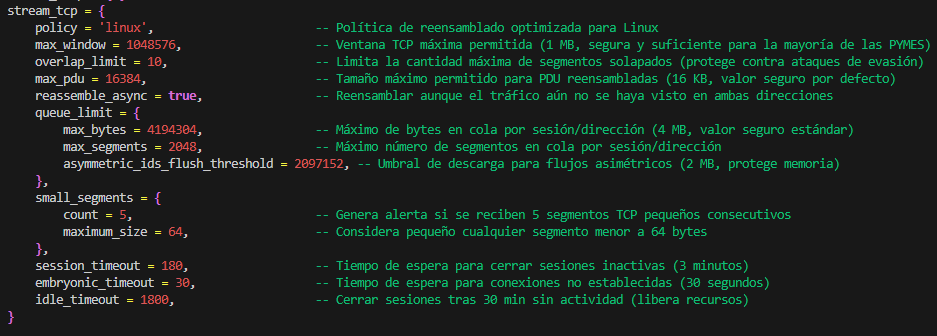
\includegraphics[scale=0.6]{stream_tcp/1.png}
	\caption{Configuración de Stream TCP.}
\end{figure}

\subsubsection*{Reputation}

Este preprocesador permite bloquear IPs clasificadas como maliciosas utilizando listas negras. Para su funcionamiento se ha creado una carpeta \texttt{/reputation}, donde se almacena un archivo con IPs sospechosas, obtenidas del repositorio de \textit{emergingthreats.net} \cite{emerging_block_ips}.  Esta funcionalidad es útil para evitar conexiones no deseadas hacia o desde nodos peligrosos.\newline

Como en los casos anteriores, tras configurar el módulo, se valida la sintaxis y se reinicia Snort para aplicar los cambios.

\begin{figure}[H]
	\centering
	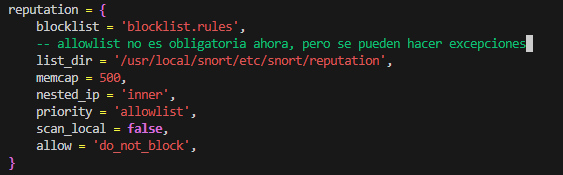
\includegraphics[scale=0.8]{reputation/1.png}
	\caption{Configuración de Reputation.}
\end{figure}

\newpage

\subsubsection*{Datos sensibles}

En versiones anteriores de Snort existía el preprocesador \textit{Sensitive Data}, pero ha sido descontinuado en las versiones más recientes. Sin embargo, es posible emular parte de su funcionalidad adaptando expresiones regulares personalizadas que alerten sobre la presencia de datos sensibles típicos en el entorno de una PYME, como credenciales o números de tarjetas.\newline

Para ello, se crea un nuevo archivo de reglas llamado \texttt{custom.rules}, donde se definen patrones específicos a detectar.

\begin{figure}[H]
	\centering
	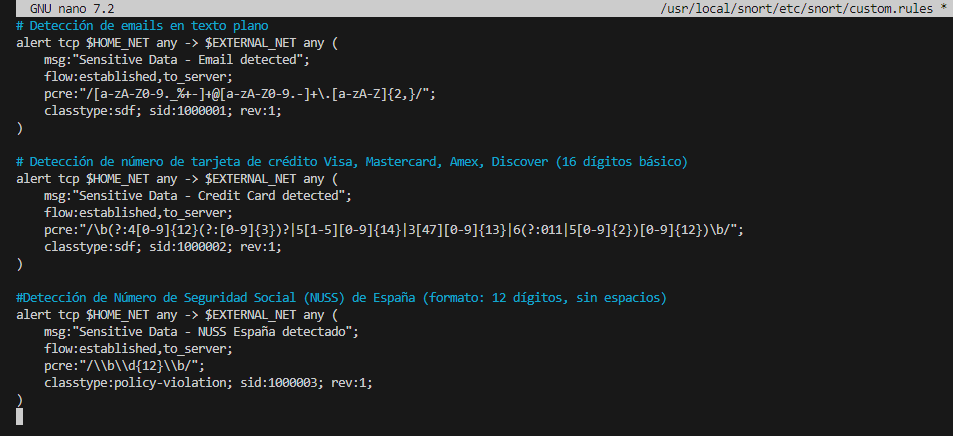
\includegraphics[scale=0.6]{sensitive/1.png}
	\caption{Expresiones regulares para protección de datos sensibles.}
\end{figure}

Posteriormente, se añade la ruta de este archivo en \texttt{snort.lua}, se comprueba la validez de la configuración utilizando \texttt{libdaq} y se reinicia el servicio para aplicar los cambios.

\begin{figure}[H]
	\centering
	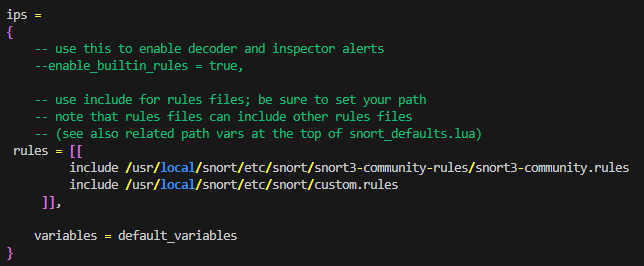
\includegraphics[scale=0.6]{sensitive/2.png}
	\caption{Agregación de \texttt{custom.rules}.}
\end{figure}

\pagebreak

\subsubsection*{Antivirus ClamAV}

Finalmente, se procede con la instalación del antivirus \textbf{ClamAV}, una solución de código abierto utilizada para la detección de malware. Su integración complementa las capacidades de Snort mediante el análisis basado en firmas.

\begin{figure}[H]
	\centering
	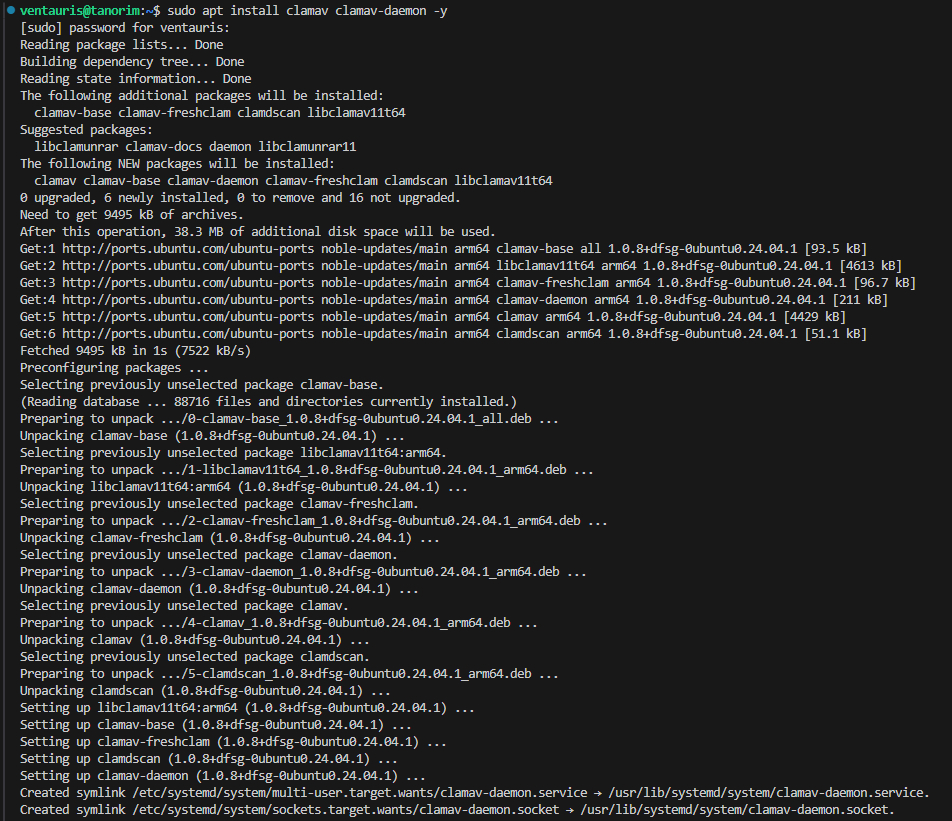
\includegraphics[scale=0.6]{clamAV/1.png}
	\caption{Instalación de ClamAV.}
\end{figure}

Tras la instalación, se detiene el servicio, se actualizan las firmas de virus y se reinicia el demonio para activar la protección.

\begin{figure}[H]
	\centering
	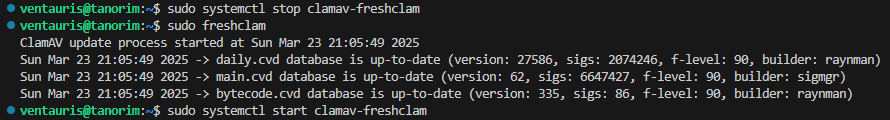
\includegraphics[scale=0.6]{clamAV/2.png}
	\caption{Actualización de firmas y reinicio del servicio ClamAV.}
\end{figure}


\newpage

%%%%%%%%%%%%%%%%%%HECHO5

\section{Generación de un script para la instalación automática}

\subsection{Esquema de red de monitorización con R-SNORT}

\begin{figure}[H]
	\centering
	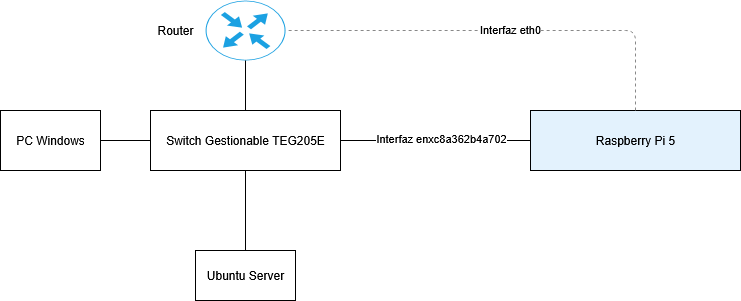
\includegraphics[scale=0.6]{script_automatico/network.png}
	\caption{Esquema de red real del proyecto.}
\end{figure}

El \textit{Port Mirroring} se configura para duplicar el tráfico de los puertos 1, 2 y 3 (los dispositivos productivos y el router) hacia el puerto 4, permitiendo que la interfaz \texttt{enxc8a362b4a702} de la Raspberry Pi capture de forma pasiva y en tiempo real todo el tráfico interno y externo de la red.

\subsubsection{Objetivo de este diseño}

El objetivo principal de esta arquitectura es que \textbf{R-SNORT} funcione como un sistema de detección de intrusiones pasivo (\textit{Network-based IDS}) sin interferir en el flujo de los datos. Para ello, deben cumplirse dos condiciones técnicas fundamentales:

\begin{enumerate}
	\item La interfaz utilizada para la captura debe operar en \textbf{modo promiscuo}, sin dirección IP asignada, actuando como una sonda pasiva totalmente invisible para el resto de la red.
	\item El switch debe soportar \textbf{duplicación de tráfico} (\textit{mirroring}) para garantizar que todo el tráfico relevante sea reenviado correctamente al puerto de análisis.
\end{enumerate}

\subsubsection{Justificación técnica}

Este tipo de arquitectura es común en entornos profesionales donde se desea realizar \textit{inspección profunda de paquetes} (\textit{Deep Packet Inspection}) sin introducir latencia ni crear puntos únicos de fallo en la red \cite{song2020dpi}. Además, permite mantener completamente aislado el sistema IDS del resto de dispositivos, lo cual incrementa la seguridad del propio entorno de monitorización.\newline

La elección de una \textbf{Raspberry Pi 5} se justifica por su bajo consumo energético, su arquitectura ARM eficiente, y su capacidad para operar con interfaces Ethernet Gigabit, siempre que se utilice un adaptador USB 3.0 para incorporar una segunda interfaz de red.

\subsubsection{Alternativas descartadas}

Se valoró la posibilidad de implementar una arquitectura enrutada —donde todo el tráfico pasara a través de la Raspberry Pi—, sin embargo, esta solución presentaba varios inconvenientes:

\begin{itemize}
	\item Aumentaría la latencia y la carga de red para todos los dispositivos conectados.
	\item Requiere una configuración compleja de \texttt{NAT} o \texttt{bridging} en la Raspberry Pi.
	\item Introduce un punto único de fallo que compromete la disponibilidad de la red en caso de errores.
\end{itemize}

Por tanto, la arquitectura basada en un \textbf{switch con mirroring} y una sonda pasiva resulta significativamente más robusta, profesional y realista para el entorno de una pequeña o mediana empresa (\textbf{PYME}).


\subsection{Primera fase del script automático}
% Contenido de la sección 2.5
La instalación manual de \textit{Snort 3}, especialmente en dispositivos embebidos como la Raspberry Pi, puede convertirse en un proceso complejo y propenso a errores debido a la cantidad de dependencias, compilaciones desde código fuente y configuraciones específicas del sistema. Por este motivo, se ha desarrollado un script de instalación automática denominado \textbf{R-SNORT INSTALLER}, que encapsula todo el proceso de despliegue de manera modular, robusta y reproducible.

\subsubsection{Motivación y diseño modular}

Automatizar la instalación de herramientas en ciberseguridad como Snort es un paso habitual para garantizar la repetibilidad de los entornos de prueba, minimizar el error humano y facilitar la portabilidad entre dispositivos. Esta filosofía está alineada con los principios de \textit{Infrastructure as Code} (IaC), promovida en múltiples estudios recientes sobre automatización segura.
\newline

El script propuesto sigue una arquitectura modular, dividiendo su lógica en funciones independientes organizadas en ficheros temáticos:

\begin{itemize}
	\item \texttt{r-snort\_installer.sh}: Núcleo del sistema, orquesta las fases del proceso de instalación desde una perspectiva modular, gestionando logs, permisos, selección de interfaz y llamadas a los demás módulos.  
	Véase el Código~\ref{lst:r-snort-installer} para una muestra del flujo de ejecución principal.
	
	\item \texttt{core.sh}: Módulo responsable de los mensajes de log, errores y el banner de bienvenida, garantizando una salida legible y profesional para el usuario.  
	Véase el Código~\ref{lst:core-sh}.
	
	\item \texttt{checks.sh}: Este módulo verifica que el script se ejecute como root y solicita al usuario que seleccione la interfaz de red sobre la que actuará Snort.  
	Representación visual en la Figura~\ref{lst:checks-sh}.
	
	\item \texttt{dependencies.sh}: Instala los paquetes de compilación y bibliotecas necesarios en entornos Debian/Ubuntu.  
	El Código~\ref{lst:dependencies-sh} muestra esta lógica.
	
	\item \texttt{build\_from\_source.sh}: Gestiona y compila desde fuentes los componentes adicionales (luajit, daq, openssl, etc.).  
	También maneja errores comunes de compatibilidad, como se muestra a continuación:
	
	\begin{lstlisting}[language=bash, caption={Corrección de versiones incompatibles de xz/liblzma}, label=lst:xz, basicstyle=\ttfamily\footnotesize, frame=single, numbers=left, numberstyle=\tiny, breaklines=true]
		if ! xz -t "$archivo" 2>&1 | grep -qv 'version `XZ_'; then
		apt-get install --reinstall -y xz-utils liblzma5 liblzma-dev
		fi
	\end{lstlisting}
	
	\item \texttt{install\_snort.sh}: Compila Snort 3.1.84.0 con correcciones específicas para evitar fallos con versiones recientes de OpenSSL y desactiva el soporte NUMA.  
	Véase el Código~\ref{lst:install-snort}.
	
	\item \texttt{configure\_snort.sh}: Prepara la configuración final de Snort, cargando reglas, scripts \texttt{.lua}, y desplegando el servicio con \texttt{systemd}.  
	Representado en el Código~\ref{lst:configure-snort}.
	
	\item \texttt{swap.sh}: Activa dinámicamente un archivo de swap temporal si se detecta menos de 1.5\,GB de RAM, evitando fallos de compilación en la Raspberry Pi.  
	Ver el Código~\ref{lst:swap-sh}.
	
	\item \texttt{stats.sh}: Recopila y presenta estadísticas del sistema tras la instalación, incluyendo versiones de Snort y ClamAV, recursos utilizados y configuración de red.  
	Ilustrado en el Código~\ref{lst:stats-sh}.
\end{itemize}

\subsubsection{Características de robustez y control de errores}

El script implementa buenas prácticas de scripting en Bash, incluyendo:

\begin{itemize}
	\item Uso de \texttt{set -euo pipefail} para evitar ejecuciones silenciosas tras errores.
	\item Captura de errores con \texttt{trap} para identificar fallos que desestabilicen o anulen la instalación.
	\item Registro detallado en \texttt{/var/log/snort\_install.log} mediante redirección directa del flujo de salida.
\end{itemize}

Además, cada función de especial importancia o con condiciones de carrera se acompaña de validaciones explícitas. Por ejemplo, antes de descomprimir archivos \texttt{.tar.gz} o \texttt{.tar.xz}, se comprueba su integridad con \texttt{gzip -t} o \texttt{xz -t}, y se mitigan fallos comunes de \texttt{liblzma} con reinstalación forzada si es necesario.

\begin{lstlisting}[language=bash, caption={Validación e instalación segura de paquetes xz}, label="lst:xz"]
	if ! xz -t "\$archivo" 2>&1 | grep -qv 'version `XZ_'; then
	apt-get install --reinstall -y xz-utils liblzma5 liblzma-dev
	fi
\end{lstlisting}

\subsubsection{Automatización total del servicio Snort}

Una vez instalado, \texttt{Snort} es configurado automáticamente como un servicio \texttt{systemd}. El script genera dinámicamente el archivo \texttt{snort.service} y lo enlaza al directorio correcto, con los parámetros adecuados de reinicio automático, límites de recursos y uso de la interfaz de red seleccionada interactivamente por el usuario.

\begin{lstlisting}[language=bash, caption={Sección relevante del systemd generado}, label=lst:systemd]
	[Service]
	ExecStart=/usr/local/snort/bin/snort -c /usr/local/snort/etc/snort/snort.lua -i eth0 -A alert_fast
	Restart=always
	User=root
	Group=root
\end{lstlisting}

\subsubsection{Mitigación de limitaciones de hardware}

Para abordar las limitaciones de memoria RAM propias de sistemas como la ARM (no presente en Raspberry Pi 5 de 8GB de RAM), el script evalúa si el sistema posee menos de 1.5GB de RAM y en ese caso crea un archivo de swap temporal de 2GB:

\begin{lstlisting}[language=bash]
	if [ "$mem_kb" -lt 1500000 ]; then
	fallocate -l 2G /swapfile_snort
\end{lstlisting}

Esta característica permite compilar Snort de forma estable incluso en configuraciones reducidas, evitando fallos durante la fase de \texttt{make -j\$(nproc)}.

\subsubsection{Instalación adicional de ClamAV y control antivirus}

Dado que el proyecto R-Snort está pensado como un sistema IDS autónomo para pequeñas y medianas empresas, se incluyó también la instalación automática de \texttt{ClamAV}, permitiendo disponer de un escáner antivirus activo desde el arranque. La instalación es completamente silenciosa y actualiza su base de firmas mediante \texttt{freshclam}.

\subsubsection{Resultados e impacto del diseño}

El instalador automático consigue reducir a menos de 15 minutos la instalación completa de Snort, desde dependencias hasta configuración funcional. Esta reducción de complejidad aumenta la fiabilidad y la reproducibilidad del entorno, dos factores muy demandados para sistemas de detección de intrusos.\newline

Además, se ha verificado que, tras una ejecución limpia del instalador, Snort queda operativo como servicio persistente, escuchando tráfico en tiempo real y generando alertas sobre tráfico malicioso, todo ello sin intervención posterior del usuario.

\pagebreak

%%%%%%%%%%%%HECHO6

\subsection{Transición a paquete \texttt{.deb}}

Con el objetivo de profesionalizar el despliegue de \textbf{R-SNORT} y facilitar su uso en entornos reales, se reestructuró el proyecto como un paquete Debian estándar. Esta decisión permite que el propio sistema operativo gestione la instalación, dependencias, configuración y servicio a través de scripts como \texttt{postinst} (ver Código~\ref{lst:postinst}), \texttt{prerm} (ver Código~\ref{lst:prerm}) y \texttt{postrm} (ver Código~\ref{lst:postrm}), alineándose con las buenas prácticas del ecosistema Debian \cite{debian_packaging_guide}.
\newline

El resultado es una arquitectura empaquetada bajo el nombre \texttt{r-snort-deb.deb}, que se instala fácilmente mediante un único comando y permite revertir el proceso de instalación sin dejar rastros en el sistema.

\begin{figure}[H]
	\centering
	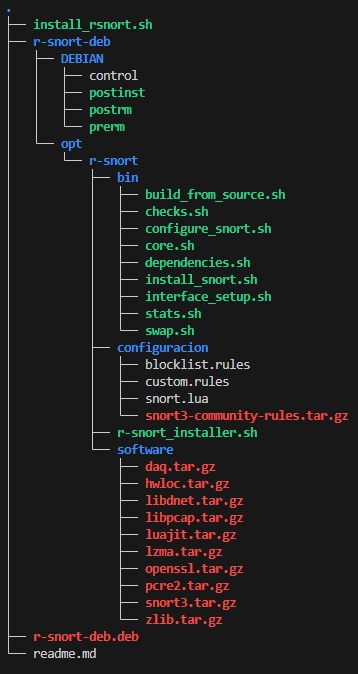
\includegraphics[scale=0.8]{script_automatico/13.png}
	\caption{Estructura del proyecto reempaquetado como archivo \texttt{.deb}.}
\end{figure}

\pagebreak

\subsubsection{Mejoras introducidas}

La transición al formato \texttt{.deb} permitió incorporar una serie de mejoras que anteriormente solo podían aplicarse de forma manual:

\begin{itemize}
	\item \textbf{Selección dinámica de interfaz:} Se desarrolló un script de instalación previa, \textbf{install\_rsnort.sh} (ver Código~\ref{lst:install-rsnort}), que detecta automáticamente las interfaces Ethernet disponibles y permite al usuario seleccionar la que se conectará al puerto espejo del switch. La elección se guarda en \texttt{/etc/rsnort\_iface} para que pueda ser utilizada posteriormente por otros componentes del sistema.
	
	\item \textbf{Modo promiscuo y sin IP:} Se creó el script \textbf{interface\_setup.sh} (ver Código~\ref{lst:interface-setup}) que activa automáticamente la interfaz seleccionada, elimina cualquier dirección IP existente para evitar conflictos, y la configura en modo \textit{promiscuo}. Este paso es esencial para que Snort pueda inspeccionar todo el tráfico redirigido desde el switch sin interferir en el funcionamiento de la red.
	
	\begin{lstlisting}[language=bash, caption={Activación automática del modo promiscuo en interface\_setup.sh}, label=lst:promiscuo, basicstyle=\ttfamily\footnotesize, frame=single, numbers=left, numberstyle=\tiny, breaklines=true]
	if [[ "$state" != "UP" ]]; then
		ip link set dev "$iface" up
	fi
	
	ip addr flush dev "$iface"
	ip link set "$iface" promisc on
	\end{lstlisting}
	
	\item \textbf{Despliegue como servicio \texttt{systemd}:} Se redefinió el proceso de inicio de Snort mediante una unidad personalizada de \texttt{systemd}, lo que permite un arranque automático, supervisión y control del servicio tras cada reinicio del sistema.
	
	\item \textbf{Fortalecimiento con ClamAV:} Para añadir una capa extra de protección, se integró la instalación y activación automática del antivirus ClamAV. Esto es especialmente útil en entornos donde Snort pueda capturar tráfico de archivos potencialmente contaminados o vectores de malware.
\end{itemize}

\subsubsection{Justificación del rediseño}

Este rediseño responde no solo a criterios técnicos, sino también a aspectos de usabilidad. En entornos reales, como pequeñas y medianas empresas (PYMEs), que desean adoptar soluciones \textit{NIDS}, es esencial que la herramienta pueda instalarse, configurarse y mantenerse sin requerir conocimientos avanzados en administración de sistemas. Gracias a esta transición, \textbf{R-SNORT} puede considerarse una solución \textit{plug-and-play}:

\begin{enumerate}
	\item El usuario ejecuta \texttt{install\_rsnort.sh}.
	\item Selecciona la interfaz conectada al switch mediante un menú interactivo.
	\item El paquete se instala y configura automáticamente, sin intervención adicional.
\end{enumerate}

Esta arquitectura modular empaquetada sigue las mejores prácticas de la ingeniería de software y permite escalar, actualizar o personalizar R-SNORT en futuras versiones con mínima fricción.

\pagebreak

\subsubsection{Resultado final}

Gracias a la evolución hacia un paquete \texttt{.deb}, \textbf{R-SNORT} se consolida como una herramienta más robusta, mantenible y amigable con el usuario final. Es importante recordar que este proyecto busca ofrecer una solución eficaz, ligera y accesible para redes SOHO (\textit{Small Office / Home Office}). Con un enfoque modular interno y una experiencia de instalación unificada, el sistema mantiene toda su capacidad de inspección avanzada sin renunciar a la simplicidad en su despliegue.

%HECHO7


\chapter{Caso práctico: utilización de R-Snort}

\section{Entorno de trabajo}

El sistema R-Snort ha sido desplegado en un entorno de red realista a pequeña escala, compuesto por los siguientes elementos:

\begin{itemize}
	\item Una Raspberry Pi 5 con sistema operativo Ubuntu Server, encargada de ejecutar el paquete automatizado con Snort.
	\item Un switch gestionable Tenda TEG205E, configurado para replicar todo el tráfico de red mediante la funcionalidad de \textit{port mirroring}.
	\item Un adaptador UGREEN USB 3.0 a Ethernet Gigabit conectado a la Raspberry, que actúa como interfaz de captura para Snort.
	\item Un router doméstico (F@st 5670) que proporciona conectividad a Internet a toda la red.
	\item Dos equipos cliente: un PC con Windows y otro con Ubuntu Server, ambos conectados al switch.
\end{itemize}

\begin{figure}[H]
	\centering
	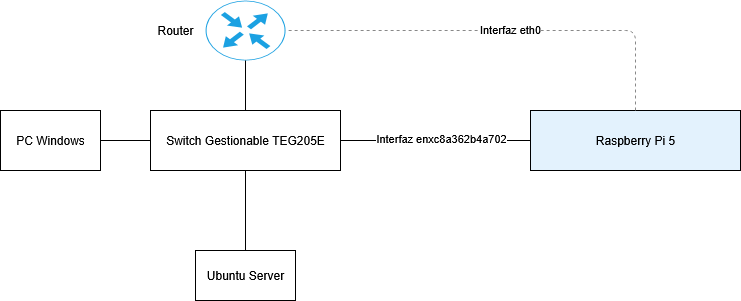
\includegraphics[scale=0.6]{script_automatico/network.png}
	\caption{Esquema de red real del proyecto.}
\end{figure}

El puerto 4 del switch se ha configurado como destino del \textit{mirroring}, recibiendo una copia del tráfico de los puertos 1 a 3 (correspondientes al router y los dos PCs). De esta manera, R-Snort es capaz de recibir una copia tanto del tráfico interno como del proveniente de Internet. La Raspberry escucha dicho tráfico a través del adaptador UGREEN, el cual se configura automáticamente en modo promiscuo, sin dirección IP asignada, para evitar interferencias en la red.

\section{Instalación}

La instalación se ha simplificado al máximo para que cualquier usuario pueda desplegar R-Snort sin conocimientos técnicos avanzados. El proceso consta de dos fases principales:

\begin{enumerate}
	\item Ejecución del script \texttt{install\_rsnort.sh}, que actualiza paquetes, instala dependencias y solicita al usuario que seleccione la interfaz de red conectada al switch.
	\item Instalación del paquete \texttt{.deb}, que compila Snort y sus dependencias, configura la interfaz en modo promiscuo, crea el servicio en \texttt{systemd}, e inicia automáticamente el demonio de Snort.
\end{enumerate}

A continuación, se presentan algunas capturas del proceso, incluyendo tanto la preparación del hardware como de la instalación software:\newline

La Raspberry Pi 5 cuenta con dos interfaces Ethernet: una conectada directamente al router para acceder a Internet desde fuera de la red local (\texttt{eth0}), y otra a través de un adaptador USB 3.0 (UGREEN) destinada exclusivamente a capturar tráfico de red (\texttt{enxc8a362b4a702}). Esta segunda interfaz es la que recibe todo el tráfico replicado desde el switch mediante \textit{port mirroring}.

\begin{figure}[H]
	\centering
	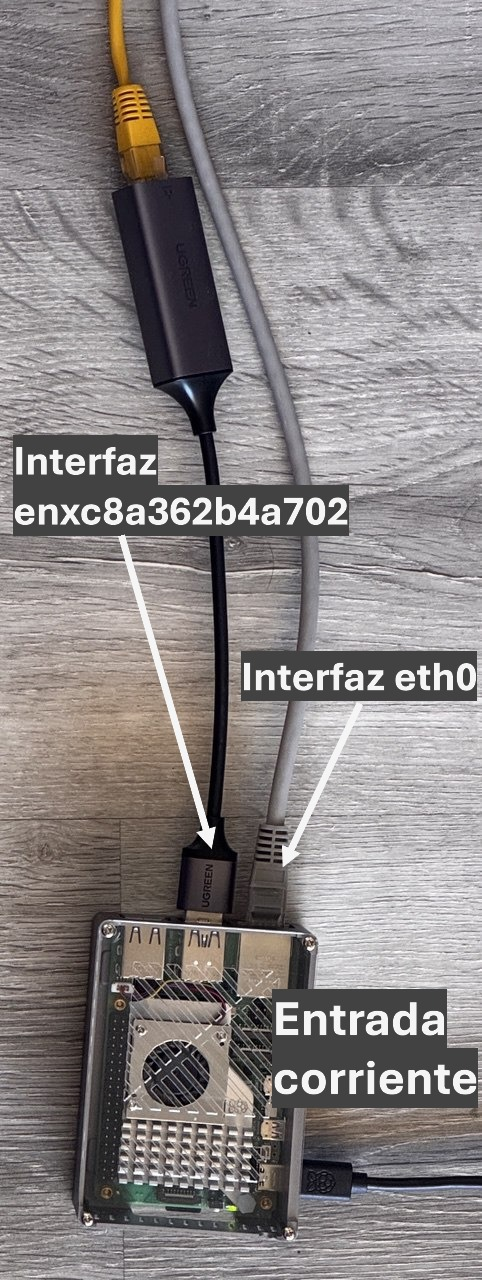
\includegraphics[width=0.3\textwidth]{pruebas_config/1-1.JPG}
	\caption{Raspberry Pi conectada con dos interfaces Ethernet.}
\end{figure}

\pagebreak

\subsection*{Asignación de dispositivos al switch}

El switch gestionable Tenda permite configurar el tráfico de cada puerto. En este caso, se conectaron el router, los dos PCs (Windows y Ubuntu Server) y la Raspberry Pi. Esta última se conecta a un puerto configurado como espejo de los demás, lo que le permite capturar el tráfico replicado.

\begin{figure}[H]
	\centering
	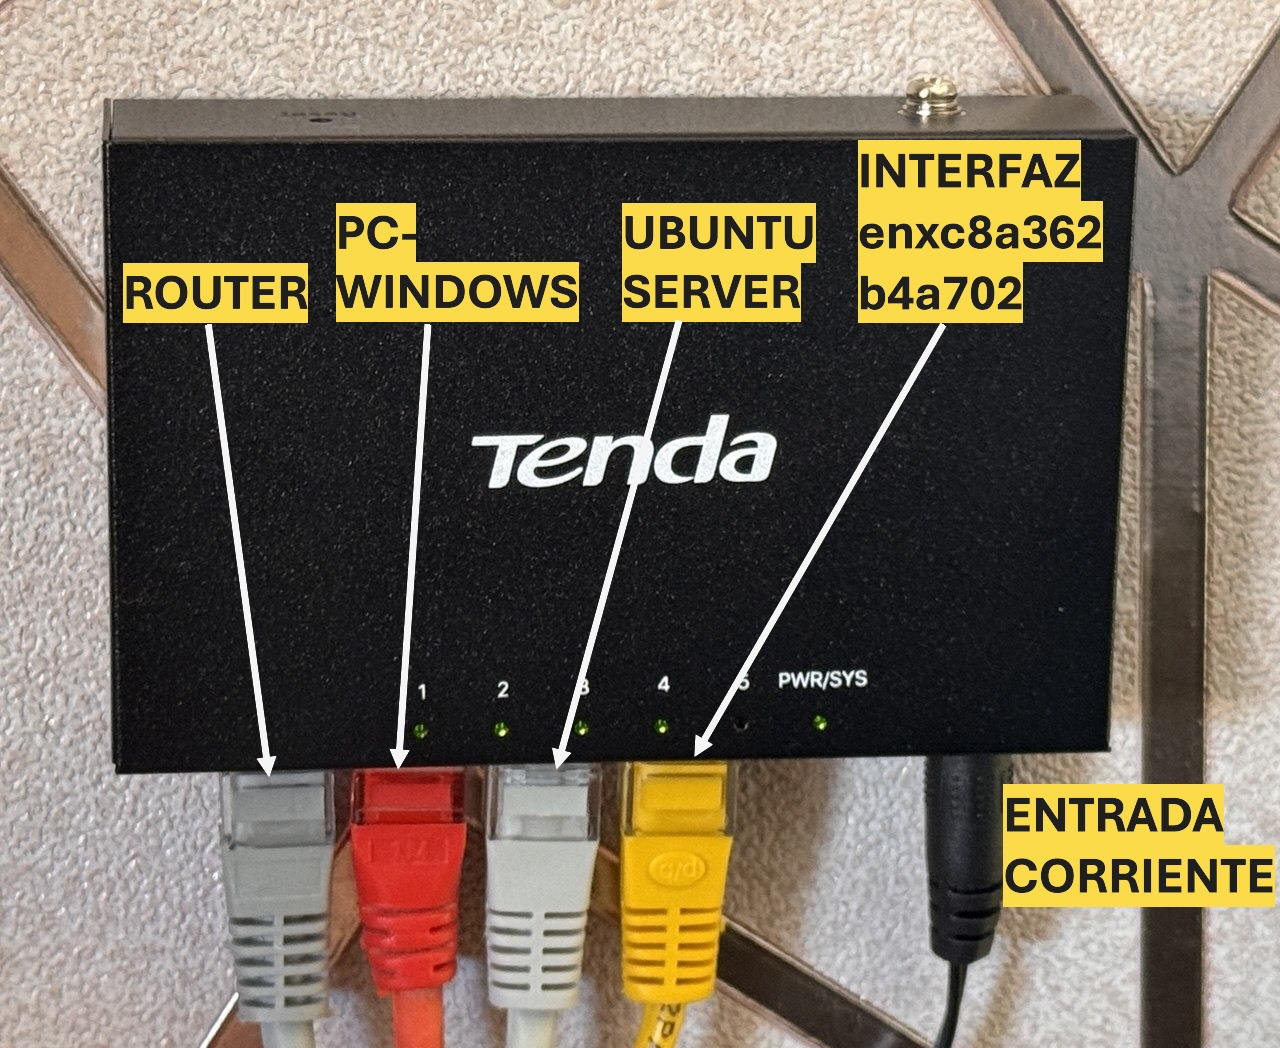
\includegraphics[width=0.65\textwidth]{pruebas_config/2-2.JPG}
	\caption{Conexiones físicas al switch gestionable.}
\end{figure}

\subsection*{Identificación del entorno LAN}

Desde la interfaz web del router se pueden visualizar todos los dispositivos conectados. Esto permite verificar que tanto el switch como la Raspberry Pi están correctamente integrados en la red y responden a su dirección IP.

\begin{figure}[H]
	\centering
	\includegraphics[width=0.65\textwidth]{pruebas_config/3-router.png}
	\caption{Dispositivos visibles en la red doméstica.}
\end{figure}

\subsection*{Acceso al switch Tenda}

Para configurar el port mirroring es necesario acceder al panel web del switch. Para ello, se localiza su dirección IP desde el router (192.168.1.169) y se accede a ella mediante un navegador web.

\begin{figure}[H]
	\centering
	\includegraphics[width=0.65\textwidth]{pruebas_config/4-localizar_tenda.png}
	\caption{IP local del switch detectada desde el router.}
\end{figure}

\begin{figure}[H]
	\centering
	\includegraphics[width=0.5\textwidth]{pruebas_config/5-tenda_web.png}
	\caption{Pantalla de acceso al panel de administración.}
\end{figure}

\subsection*{Seguridad inicial del dispositivo}

En el primer acceso al switch, el sistema solicita el cambio obligatorio de la contraseña predeterminada para mejorar la seguridad del entorno.

\begin{figure}[H]
	\centering
	\includegraphics[width=0.5\textwidth]{pruebas_config/6-cambio_pass_tenda.png}
	\caption{Cambio obligatorio de contraseña en el primer inicio.}
\end{figure}

\subsection*{Configuración avanzada del switch}

Una vez autenticados, accedemos a la interfaz de administración, donde es posible configurar diversos parámetros del dispositivo. Desde esta sección se define el \textit{port mirroring}, se habilitan o deshabilitan puertos y se monitoriza el estado de la red.

\begin{figure}[H]
	\centering
	\includegraphics[width=0.8\textwidth]{pruebas_config/7-pagina_tenda.png}
	\caption{Vista general del panel de gestión del switch.}
\end{figure}

\subsection*{Activación del Port Mirroring}

Desde el apartado \texttt{switching > port mirroring}, activamos esta funcionalidad para duplicar el tráfico de red. Se configura el switch para replicar el tráfico de los puertos donde están conectados el router y los PCs (puertos 1, 2 y 3) hacia el puerto 4, que está vinculado a la interfaz de análisis de la Raspberry Pi. Esto permite que Snort reciba una copia completa del tráfico local y externo.

\begin{figure}[H]
	\centering
	\includegraphics[width=0.8\textwidth]{pruebas_config/9-asignacion_port.png}
	\caption{Verificación del estado de los puertos tras la configuración.}
\end{figure}

Una vez la Raspberry Pi 5 sea capaz de recibir todo el tráfico en modo espejo por la interfaz correspondiente de toda la red local al mismo tiempo que tiene conexión a internet externo por la interfaz predeterminada del sistema se pone en marcha el paquete automatizado para instalar la Snort junto con la configuración completa.\newline

Finalmente, ejecutamos como administrador el script \texttt{installer\_snort.sh} para iniciar la instalación de R-Snort. Se selecciona la interfaz de red correspondiente al puerto 4 del switch, que es el que recibe el tráfico duplicado \cite{bartman2016snort}. Una vez finalizado el proceso, el sistema queda completamente operativo. El código fuente del instalador puede consultarse en el Anexo~\ref{anexo_repositorio}.

\begin{figure}[H]
	\centering
	\begin{minipage}[b]{0.48\textwidth}
		\centering
		\includegraphics[scale=0.35]{script_automatico/14.png}
		\caption*{(a) Ejecución de R-Snort.}
	\end{minipage}
	\hfill
	\begin{minipage}[b]{0.48\textwidth}
		\centering
		\includegraphics[scale=0.35]{pruebas_config/10-10.png}
		\caption*{(b) Finalización del instalador.}
	\end{minipage}
	\caption{Proceso completo de instalación automática de R-Snort.}
\end{figure}

\pagebreak

%HECHO8

% --> Aquí se insertan las figuras

\section{Utilización y pruebas}

Una vez completada la instalación, se procedió a la validación funcional del sistema y a su evaluación de rendimiento. El objetivo principal es demostrar que R-Snort es capaz de monitorizar eficazmente el tráfico de red y detectar amenazas sin sobresaturar los recursos del sistema.

\subsection{Pruebas de validación del funcionamiento}

\subsubsection*{Prueba 1: Preprocesadores \texttt{stream}, \texttt{stream\_ip} e \texttt{icmp}}

\textbf{Objetivo:} \\
Comprobar el funcionamiento de los preprocesadores \texttt{stream}, \texttt{stream\_ip} e \texttt{icmp}, así como la capacidad del sistema R-Snort para detectar múltiples patrones relacionados con tráfico ICMP anómalo o sospechoso.\newline

\textbf{Descripción de la prueba:} \\
Desde el equipo Ubuntu Server (\texttt{192.168.1.133}) se ejecutó un comando \texttt{ping} con valor TTL bajo hacia el servidor DNS público de Google (\texttt{8.8.8.8}), lo que genera tráfico susceptible de ser clasificado como malicioso o anómalo.

\begin{lstlisting}[style=commandstyle]
	ping -t 1 8.8.8.8
\end{lstlisting}

Este tipo de tráfico ICMP con TTL muy bajo es común en herramientas de escaneo y técnicas de reconocimiento como \texttt{traceroute}, por lo que debe ser identificado por un sistema de detección de intrusos.\newline

\textbf{Resultado:} \\
R-Snort detectó correctamente el tráfico como potencialmente sospechoso. A continuación se muestra una tabla con algunas de las alertas generadas:

\begin{table}[H]
	\centering
	\resizebox{\textwidth}{!}{%
		\begin{tabular}{|l|l|l|l|l|}
			\hline
			\textbf{Timestamp} & \textbf{Protocolo} & \textbf{Origen} & \textbf{Destino} & \textbf{Mensaje de alerta} \\
			\hline
			17:45:54 & ICMP & 192.168.1.133 & 8.8.8.8 & PROTOCOL-ICMP PING Unix \\
			17:45:54 & ICMP & 192.168.1.133 & 8.8.8.8 & PROTOCOL-ICMP Unusual PING detected \\
			17:45:54 & ICMP & 192.168.1.133 & 8.8.8.8 & PROTOCOL-ICMP traceroute \\
			17:45:54 & ICMP & 192.168.1.1 & 192.168.1.133 & PROTOCOL-ICMP Time-To-Live Exceeded \\
			\hline
		\end{tabular}%
	}
	\caption{Alertas ICMP generadas durante la prueba de TTL bajo.}
\end{table}

\begin{figure}[H]
	\centering
	\includegraphics[width=0.9\textwidth]{pruebas_bien/seccion_uno/1.png}
	\caption{Fragmento de alertas generadas por tráfico ICMP anómalo.}
\end{figure}

Esta prueba demuestra que el sistema R-Snort no solo detecta tráfico ICMP, sino que lo analiza correctamente comportamientos inusuales, patrones tipo \texttt{traceroute} y errores de TTL. El resultado valida tanto la activación de los preprocesadores como la integración de las reglas comunitarias.

\subsubsection*{Prueba 2: Preprocesadores \texttt{stream\_tcp} y \texttt{http\_inspect}}

\textbf{Objetivo:} \\
Comprobar el funcionamiento de los preprocesadores \texttt{stream\_tcp} y \texttt{http\_inspect}, verificando si el sistema R-Snort es capaz de identificar comportamientos anómalos asociados a solicitudes HTTP con cabeceras excesivamente largas.\newline

\textbf{Descripción de la prueba:} \\
Desde el equipo Ubuntu Server (\texttt{192.168.1.133}) se generó una solicitud HTTP con una cabecera personalizada de 6000 caracteres. Este tipo de tráfico puede ser usado para evadir mecanismos de inspección o insertar código malicioso en el servidor receptor.

\begin{lstlisting}[style=commandstyle]
	curl -H "X-Test: $(printf '%0.sA' {1..6000})" http://192.168.1.1
\end{lstlisting}

Aunque el objetivo era activar una alerta por cabecera anómala, Snort reaccionó con una alerta más severa al detectar un patrón característico de shellcode, mostrando así un nivel de análisis más profundo.\newline

\textbf{Resultado:} \\
R-Snort generó múltiples alertas clasificadas como shellcode (`INDICATOR-SHELLCODE`), lo cual valida la efectividad del sistema ante posibles vectores de ataque que podrían comprometer la seguridad de una red.

\begin{table}[H]
	\centering
	\resizebox{\textwidth}{!}{%
		\begin{tabular}{|l|l|l|l|l|}
			\hline
			\textbf{Timestamp} & \textbf{Protocolo} & \textbf{Origen} & \textbf{Destino} & \textbf{Mensaje de alerta} \\
			\hline
			19:07:54 & TCP & 192.168.1.133 & 192.168.1.1 & INDICATOR-SHELLCODE x86 inc ecx NOOP \\
			19:07:54 & TCP & 192.168.1.133 & 192.168.1.1 & INDICATOR-SHELLCODE x86 inc ecx NOOP \\
			19:07:54 & TCP & 192.168.1.133 & 192.168.1.1 & INDICATOR-SHELLCODE x86 inc ecx NOOP \\
			\hline
		\end{tabular}%
	}
	\caption{Alertas generadas por tráfico HTTP con cabecera anómala interpretado como shellcode.}
\end{table}

\begin{figure}[H]
	\centering
	\includegraphics[width=0.9\textwidth]{pruebas_bien/seccion_uno/2.png}
	\caption{Detección de shellcode.}
\end{figure}

Esta prueba valida que R-Snort es capaz de analizar en profundidad el contenido de las cabeceras HTTP y detectar patrones que puedan representar intentos de explotación o evasión. Aunque la alerta no fue específicamente la esperada, el resultado demuestra un comportamiento más inteligente y proactivo en la inspección de tráfico.

\subsubsection*{Prueba 3: Preprocesador \texttt{dns}}

\textbf{Objetivo:} \\
Verificar el funcionamiento del preprocesador \texttt{dns} y la capacidad de R-Snort para detectar respuestas DNS anómalas, como aquellas con TTL bajo y sin autoridad, lo cual es característico de intentos de suplantación o respuestas manipuladas.\newline

\textbf{Descripción de la prueba:} \\
Desde el equipo Ubuntu Server (\texttt{192.168.1.133}) se ejecutó una consulta DNS directa al servidor público de Google utilizando el comando \texttt{dig}. Esta prueba simula una resolución común que puede generar respuestas mínimas o manipuladas desde el servidor, activando reglas de detección de spoofing.

\begin{lstlisting}[style=commandstyle]
	dig +noall +answer google.com @8.8.8.8
\end{lstlisting}

\textbf{Resultado:} \\
Snort generó correctamente varias alertas clasificadas como tráfico DNS sospechoso. Estas alertas corresponden a respuestas con TTL muy bajo y sin registros de autoridad, lo cual puede indicar un intento de manipulación de DNS.

\begin{table}[H]
	\centering
	\resizebox{\textwidth}{!}{%
		\begin{tabular}{|l|l|l|l|l|}
			\hline
			\textbf{Timestamp} & \textbf{Protocolo} & \textbf{Origen} & \textbf{Destino} & \textbf{Mensaje de alerta} \\
			\hline
			19:19:17 & UDP & 46.6.113.34 & 192.168.1.134 & PROTOCOL-DNS SPOOF ... and no authority \\
			19:19:21 & UDP & 46.6.113.34 & 192.168.1.134 & PROTOCOL-DNS SPOOF ... and no authority \\
			\hline
		\end{tabular}%
	}
	\caption{Alertas DNS generadas por respuestas con TTL bajo y sin autoridad.}
\end{table}

\begin{figure}[H]
	\centering
	\includegraphics[width=0.9\textwidth]{pruebas_bien/seccion_uno/3.png}
	\caption{Fragmento mostrando respuestas DNS sospechosas.}
\end{figure}

Esta prueba valida que el preprocesador \texttt{dns} está activo y funcional, siendo capaz de identificar anomalías comunes en el tráfico DNS que podrían indicar intentos de suplantación o evasión.

\subsubsection*{Prueba 4: Preprocesadores \texttt{rpc\_decode} y \texttt{snmp}}

\textbf{Objetivo:} \\
Evaluar la capacidad del sistema R-Snort para detectar tráfico relacionado con el protocolo SNMP, comúnmente utilizado en tareas de monitorización, pero también explotado en fases de reconocimiento mediante escaneos UDP dirigidos.\newline

\textbf{Descripción de la prueba:} \\
Desde el equipo Ubuntu Server (\texttt{192.168.1.133}) se lanzó un escaneo UDP contra el router de la red local, con el objetivo de identificar servicios SNMP activos:

\begin{lstlisting}[style=commandstyle]
	sudo nmap -sU -p 161,705 192.168.1.1
\end{lstlisting}

Este tipo de exploración intenta conectarse a los puertos SNMP estándar y AgentX, generando tráfico anómalo que debería activar alertas en los preprocesadores \texttt{snmp} y \texttt{rpc\_decode}.\newline

\textbf{Resultado:} \\
Snort detectó múltiples intentos de conexión hacia los puertos SNMP y generó alertas asociadas tanto a peticiones como a traps UDP:

\begin{table}[H]
	\centering
	\resizebox{\textwidth}{!}{%
		\begin{tabular}{|l|l|l|l|l|}
			\hline
			\textbf{Timestamp} & \textbf{Protocolo} & \textbf{Origen} & \textbf{Destino} & \textbf{Mensaje de alerta} \\
			\hline
			19:44:33 & UDP & 192.168.1.133 & 192.168.1.1:161 & PROTOCOL-SNMP request udp \\
			19:44:33 & UDP & 192.168.1.133 & 192.168.1.1:705 & PROTOCOL-SNMP trap udp \\
			19:44:33 & UDP & 192.168.1.133 & 192.168.1.1:705 & PROTOCOL-SNMP request udp \\
			19:44:34 & UDP & 192.168.1.133 & 192.168.1.1:161 & PROTOCOL-SNMP request udp \\
			\hline
		\end{tabular}%
	}
	\caption{Alertas generadas durante el escaneo SNMP contra el router.}
\end{table}

\begin{figure}[H]
	\centering
	\includegraphics[width=0.9\textwidth]{pruebas_bien/seccion_uno/4.png}
	\caption{Fragmento de las alertas SNMP generadas por el escaneo con Nmap.}
\end{figure}

Esta prueba valida el correcto funcionamiento de los preprocesadores \texttt{snmp} y \texttt{rpc\_decode}, así como la integración eficaz de las reglas comunitarias orientadas a protocolos de red clásicos.

\subsubsection*{Prueba 5: Reglas personalizadas de detección de datos sensibles}

\textbf{Objetivo:} \\
Comprobar el funcionamiento de las tres reglas personalizadas añadidas al archivo \texttt{custom.rules}, diseñadas para detectar información confidencial en texto plano: direcciones de correo electrónico, números de tarjeta de crédito y números de la Seguridad Social (NUSS).\newline

\textbf{Descripción de la prueba:} \\
Desde el equipo Ubuntu Server (\texttt{192.168.1.133}) se simuló una fuga de datos sensibles mediante una petición HTTP POST conteniendo simultáneamente un correo electrónico, un número de tarjeta y un NUSS.

\begin{lstlisting}[style=commandstyle]
	curl -d "Mi email es prueba@ejemplo.com. Mi tarjeta es 4111111111111111 y mi NUSS es 123456789012" http://192.168.1.1
\end{lstlisting}

Las reglas utilizadas para esta prueba fueron desarrolladas utilizando expresiones regulares (\texttt{pcre}) y se encuentran activas en el archivo \texttt{snort.lua} bajo la sección de reglas IPS.\newline

\textbf{Resultado:} \\
Snort generó múltiples alertas, una por cada patrón detectado, confirmando la efectividad de las reglas personalizadas. A continuación se resumen las más representativas:

\begin{table}[H]
	\centering
	\resizebox{\textwidth}{!}{%
		\begin{tabular}{|l|l|l|l|l|}
			\hline
			\textbf{Timestamp} & \textbf{Protocolo} & \textbf{Origen} & \textbf{Destino} & \textbf{Mensaje de alerta} \\
			\hline
			19:54:44 & TCP & 192.168.1.133 & 192.168.1.1 & Sensitive Data - NUSS España detectado \\
			19:54:44 & TCP & 192.168.1.133 & 192.168.1.1 & Sensitive Data - Credit Card detected \\
			19:54:44 & TCP & 192.168.1.133 & 192.168.1.1 & Sensitive Data - Email detected \\
			\hline
		\end{tabular}%
	}
	\caption{Alertas generadas por reglas personalizadas de fuga de datos sensibles.}
\end{table}

\begin{figure}[H]
	\centering
	\includegraphics[width=0.9\textwidth]{pruebas_bien/seccion_uno/5.png}
	\caption{Fragmento del log con alertas generadas por datos sensibles.}
\end{figure}

Esta prueba demuestra que el sistema R-Snort es capaz de analizar el contenido del tráfico en texto plano y detectar información crítica con precisión, validando la correcta integración y activación de las reglas personalizadas.


\subsection{Pruebas de rendimiento}

\subsection*{Metodología}

Para evaluar el impacto del sistema R-Snort sobre el rendimiento de la Raspberry Pi 5, se ha empleado \textbf{Performance Co-Pilot (PCP)}\cite{pcp_project} mediante su herramienta gráfica \texttt{pmchart}. Esta permite registrar y visualizar métricas del sistema en tiempo real, incluyendo uso de CPU, consumo de memoria RAM, tráfico de red, escritura a disco y actividad del proceso de Snort.\newline

Se han diseñado dos escenarios para cada métrica:
\begin{enumerate}
	\item \textbf{Snort activo}: el servicio se encuentra ejecutándose de manera habitual, recogiendo alertas desde la interfaz de red.
	\item \textbf{Snort inactivo}: el servicio se detiene por completo, permitiendo observar la carga base del sistema operativo sin interferencias de R-Snort.
\end{enumerate}

Cada prueba tiene una duración aproximada de 3 minutos bajo condiciones normales de uso. No se induce tráfico artificial, de modo que las mediciones reflejan el consumo real de recursos en una red doméstica o de oficina típica.

\bigskip

\subsection*{Prueba 1: Uso global de CPU}

\textbf{Objetivo:}  
Evaluar el impacto del sistema R-Snort sobre el uso del procesador durante el funcionamiento en segundo plano.\newline

\textbf{Métrica monitorizada:}
\begin{itemize}
	\item \texttt{kernel.all.cpu.user} – Tiempo en espacio de usuario (amarillo).
	\item \texttt{kernel.all.cpu.sys} – Tiempo en espacio de kernel (azul).
	\item \texttt{kernel.all.cpu.idle} – Tiempo inactivo (rojo).
\end{itemize}

\begin{figure}[H]
	\centering
	\includegraphics[width=\textwidth]{pruebas_bien/seccion_dos/1.png}
	\caption{Uso global de CPU con Snort activo.}
\end{figure}

Se muestra la actividad del sistema con Snort funcionando en segundo plano. Aunque la CPU se mantiene inactiva la mayor parte del tiempo (\texttt{cpu.idle}), existe una actividad constante en espacio de usuario y kernel, provocada por el análisis de paquetes y la escritura de logs por parte de Snort.

\begin{figure}[H]
	\centering
	\includegraphics[width=\textwidth]{pruebas_bien/seccion_dos/2.png}
	\caption{Uso global de CPU con Snort desactivado.}
\end{figure}

En contraste, la Figura 7.19 presenta un patrón más estable cuando Snort está detenido. El sistema entra en estados de inactividad casi total, con mínimas interrupciones. Se aprecia una reducción en el uso de CPU.\newline

La diferencia entre ambos gráficos evidencia que Snort, incluso sin tráfico malicioso, genera una carga continua sobre la CPU aunque no es elevada.

\subsection*{Prueba 2: Uso de memoria RAM}

\textbf{Objetivo:}  
Determinar el consumo de memoria generado por el sistema R-Snort durante su ejecución pasiva, sin tráfico inducido.\newline

\textbf{Métrica monitorizada:}
\begin{itemize}
	\item \texttt{mem.util.used} – Memoria utilizada (amarillo).
	\item \texttt{mem.util.free} – Memoria libre (azul).
	\item \texttt{mem.util.cached} – Memoria en caché (rojo).
\end{itemize}

\begin{figure}[H]
	\centering
	\includegraphics[width=\textwidth]{pruebas_bien/seccion_dos/3.png}
	\caption{Uso de memoria RAM con Snort activado y posteriormente detenido.}
\end{figure}

En la primera mitad del gráfico se observa un consumo de memoria estable mientras Snort permanece activo. Al detener el servicio, se registra un ligero incremento de memoria libre y una reducción proporcional de la memoria utilizada. Este comportamiento confirma que Snort mantiene una huella en RAM constante pero no intensiva, lo que lo hace adecuado para dispositivos con recursos limitados como una Raspberry Pi.

\subsection*{Prueba 3: Actividad de red}

\textbf{Objetivo:}
Observar el comportamiento del tráfico de red con y sin la ejecución de Snort para detectar posibles variaciones atribuibles al sistema de detección.

\textbf{Métrica monitorizada:} \begin{itemize} \item \texttt{network.all.in.bytes} – Tráfico entrante en MB/s (amarillo). \item \texttt{network.all.out.bytes} – Tráfico saliente en MB/s (azul). \end{itemize}

\begin{figure}[H] \centering \includegraphics[width=\textwidth]{pruebas_bien/seccion_dos/4.png} \caption{Tráfico de red con Snort activo.} \end{figure}

En esta primera figura se observa una actividad de red con múltiples picos de tráfico entrante, por otro lado, el tráfico saliente es casi nulo, esto se debe a que actualmente la Raspberry Pi 5 no está comunicando con el exterior. Esta variabilidad en el tráfico entrante se debe a la recepción de paquetes normales y las tareas de registro de eventos por parte de Snort.

\begin{figure}[H] \centering \includegraphics[width=\textwidth]{pruebas_bien/seccion_dos/5.png} \caption{Tráfico de red con Snort desactivado.} \end{figure}

Aunque también se presentan picos, su intensidad general parece ligeramente menor. Sin embargo, no se puede establecer una correlación directa entre la ejecución de Snort y una diferencia significativa en el volumen de tráfico de red, dado que éste depende principalmente de la actividad de los dispositivos conectados. El impacto de Snort sobre esta métrica resulta, por tanto, poco concluyente.

\subsection*{Prueba 4: Actividad del disco}

\textbf{Objetivo:}  
Evaluar el impacto del sistema R-Snort sobre la escritura y lectura en disco durante su ejecución pasiva.\newline

\textbf{Métrica monitorizada:}
\begin{itemize}
	\item \texttt{disk.dev.write\_bytes[mmcblk0]} – Bytes escritos por segundo (amarillo).
	\item \texttt{disk.dev.read\_bytes[mmcblk0]} – Bytes leídos por segundo (azul).
\end{itemize}

\begin{figure}[H]
	\centering
	\includegraphics[width=\textwidth]{pruebas_bien/seccion_dos/6.png}
	\caption{Actividad de disco con Snort activo.}
\end{figure}

Con Snort funcionando, se observa una mayor frecuencia de picos en la escritura de disco. Esto es consistente con la generación continua de logs en tiempo real. Las lecturas desde disco son prácticamente inexistentes, ya que Snort opera principalmente en modo de captura y escritura.

\begin{figure}[H]
	\centering
	\includegraphics[width=\textwidth]{pruebas_bien/seccion_dos/7.png}
	\caption{Actividad de disco con Snort desactivado.}
\end{figure}

Al desactivar Snort, los picos de escritura se reducen drásticamente, quedando solo operaciones menores relacionadas con el sistema. Este cambio confirma que la carga de I/O en disco generada por R-Snort es significativa y persistente durante su ejecución pasiva.\newline

\subsection*{Prueba 6: Carga media del sistema (Load Average)}

\textbf{Objetivo:}  
Observar el impacto prolongado de R-Snort sobre la carga media del sistema, utilizando la métrica de 15 minutos para evaluar si genera acumulación de procesos en cola o saturación progresiva.\newline

\textbf{Métrica monitorizada:}
\begin{itemize}
	\item \texttt{kernel.all.load[15 minute]} – Carga promedio del sistema durante los últimos 15 minutos.
\end{itemize}

\begin{figure}[H]
	\centering
	\includegraphics[width=\textwidth]{pruebas_bien/seccion_dos/8.png}
	\caption{Carga media del sistema con y sin Snort activo (15 minutos).}
\end{figure}

En la figura se muestra la evolución de la carga media del sistema en intervalos de 15 minutos. Esta métrica representa el número promedio de procesos que están en ejecución o esperando acceso a la CPU. Dado que el sistema no está sometido a una carga pesada y Snort no induce tráfico masivo, los valores se mantienen bajos (en torno a 0.13 – 0.16), lo cual es normal en sistemas con múltiples núcleos.\newline

Aunque se aprecian pequeñas fluctuaciones, estas no son significativas ni reflejan un impacto claro de Snort. Esto confirma que el servicio no genera bloqueos o acumulación de procesos cuando opera en segundo plano bajo condiciones normales de red.

\subsection{Pruebas de rendimiento bajo carga masiva}

\textbf{Objetivo:}  
Evaluar el comportamiento del sistema R-Snort cuando es sometido a tráfico de red masivo, simulando un entorno de alta exigencia como el de una red corporativa activa o un ataque volumétrico. Estas pruebas permiten analizar la capacidad de respuesta del sistema, su consumo de recursos y la estabilidad general del entorno.\newline

\textbf{Metodología:}  
Se han lanzado múltiples flujos simultáneos desde el servidor Ubuntu (192.168.1.133) hacia la Raspberry Pi (192.168.1.132), utilizando la herramienta \texttt{iperf3} en modo UDP. Para maximizar la presión sobre el sistema, se han abierto varias sesiones en paralelo y sin limitación de pacing, aumentando así la congestión de red y la carga sobre la CPU y la memoria del sistema.

\begin{lstlisting}[language=bash,caption={Simulación de tráfico masivo desde Ubuntu Server hacia la Raspberry Pi},label={lst:trafico-masivo}]
	# Ejecutar en 4 terminales distintas
	iperf3 -c 192.168.1.132 -u -b 950M -t 600 --pacing-timer 0 -l 1470 -p 5201
	iperf3 -c 192.168.1.132 -u -b 950M -t 600 --pacing-timer 0 -l 1470 -p 5202
	iperf3 -c 192.168.1.132 -u -b 950M -t 600 --pacing-timer 0 -l 1470 -p 5203
	iperf3 -c 192.168.1.132 -u -b 950M -t 600 --pacing-timer 0 -l 1470 -p 5204
\end{lstlisting}

\subsubsection*{Prueba 1: Carga promedio del sistema (kernel.all.load)}

\textbf{Métrica monitorizada:}
\begin{itemize}
	\item \texttt{kernel.all.load[15 minute]} – Carga promedio del sistema en los últimos 15 minutos.
\end{itemize}

\begin{figure}[H]
	\centering
	\includegraphics[width=\textwidth]{pruebas_bien/seccion_tres/1.png}
	\caption{Carga promedio del sistema durante tráfico masivo.}
\end{figure}

Este gráfico representa la evolución de la carga del sistema a medida que se inducía tráfico de red extremo desde múltiples fuentes. A diferencia de las condiciones normales (donde la carga oscilaba en torno a 0.15), se observa una progresión ascendente constante hasta valores cercanos a 3.0. Esto indica que, aunque la Raspberry Pi logra mantener la estabilidad, comienza a saturarse al acercarse al límite de sus cuatro núcleos físicos.\newline

La métrica de \texttt{load average} no refleja únicamente el uso de CPU, sino también la cantidad de procesos esperando ser ejecutados, incluyendo tareas bloqueadas por I/O. Por tanto, este resultado demuestra que Snort, bajo presión, sigue funcionando sin caídas, aunque con una carga crítica sostenida que evidencia el esfuerzo del sistema por procesar, analizar y registrar grandes volúmenes de datos en tiempo real.

\subsubsection*{Prueba 2: Utilización detallada de CPU (cpu.util)}

\textbf{Métricas monitorizadas:}
\begin{itemize}
	\item \texttt{kernel.cpu.util.user} – Porcentaje de tiempo en espacio de usuario (rojo).
	\item \texttt{kernel.cpu.util.sys} – Porcentaje de tiempo en espacio de kernel (azul).
	\item \texttt{kernel.cpu.util.idle} – Porcentaje de tiempo inactivo (amarillo).
\end{itemize}

\begin{figure}[H]
	\centering
	\includegraphics[width=\textwidth]{pruebas_bien/seccion_tres/2.png}
	\caption{Utilización detallada de la CPU bajo tráfico extremo.}
\end{figure}

Este gráfico proporciona una visión más precisa del uso del procesador bajo condiciones de saturación. Se observa una clara reducción del tiempo inactivo (\texttt{idle}), que desciende a valores de entre 10\% y 20\%, en contraste con los valores habituales del sistema en reposo (superiores al 90\%).\newline

Destaca el incremento del uso en espacio de kernel (\texttt{sys}), que supera con holgura al uso en espacio de usuario. Esto es coherente con el funcionamiento de Snort, ya que el procesamiento masivo de paquetes, junto con el acceso intensivo a red y disco, requiere una mayor interacción con funciones del sistema operativo.\newline

La gráfica confirma que el sistema está operando al límite de su capacidad de procesamiento, con un reparto de carga constante y sostenido, validando el impacto real que un entorno de red cargado puede tener sobre la infraestructura de detección.

\subsection*{Prueba 3: Escritura y lectura en disco durante tráfico masivo}

\textbf{Métrica monitorizada:}
\begin{itemize}
	\item \texttt{disk.dev.write\_bytes[mmcblk0]} – Escrituras en disco (amarillo).
	\item \texttt{disk.dev.read\_bytes[mmcblk0]} – Lecturas desde disco (azul).
\end{itemize}

\begin{figure}[H]
	\centering
	\includegraphics[width=\textwidth]{pruebas_bien/seccion_tres/3.png}
	\caption{Lectura y escritura en disco durante tráfico masivo.}
\end{figure}

En comparación con la prueba equivalente en la sección de tráfico normal, esta gráfica muestra un aumento en la escritura sobre el dispositivo \texttt{mmcblk0}, con picos más frecuentes y pronunciados. Esto sugiere que, aunque la carga generada por Snort no saturó el sistema de archivos, sí incrementó el volumen de logs y alertas procesadas en tiempo real. La lectura en disco, como antes, se mantiene prácticamente nula, confirmando que el sistema actúa como un sensor que escribe alertas, pero no requiere leer grandes volúmenes de datos almacenados para su funcionamiento operativo.

\pagebreak

\chapter{Resultados}

A lo largo de las pruebas realizadas, R-Snort ha demostrado ser una herramienta eficaz para la detección de intrusos en redes SOHO, operando de forma continua en segundo plano sin interferir de manera significativa en el rendimiento general del sistema. Para evaluar su impacto, se ha realizado una batería de pruebas tanto funcionales como de rendimiento, monitorizando las métricas clave del sistema mediante la herramienta \texttt{pmchart}, parte del conjunto de \texttt{Performance Co-Pilot (PCP)}.\newline

Las gráficas generadas con \texttt{pmchart} han permitido visualizar el comportamiento del sistema en distintas condiciones: tráfico normal con Snort activo, tráfico normal con Snort desactivado, y finalmente tráfico masivo inducido. A partir de esta monitorización, se ha confirmado que el impacto sobre la CPU, la memoria y la E/S en disco es bajo en condiciones normales, manteniéndose dentro de los márgenes esperables para un sistema NIDS pasivo. Incluso en situaciones de carga elevada, Snort consigue mantenerse operativo, aunque con un incremento notable en el uso de CPU y escrituras a disco, especialmente cuando se multiplica el tráfico mediante herramientas como \texttt{iperf3}.\newline

Las pruebas funcionales con tráfico real, tanto manual como automatizado, han validado el correcto funcionamiento de los preprocesadores de Snort, así como la eficacia de las reglas comunitarias y las personalizadas definidas para este proyecto. Casos como la detección de fugas de datos (emails, tarjetas de crédito, NUSS), escaneos SNMP, respuestas DNS sospechosas o tráfico ICMP fueron correctamente identificados y registrados. Esto respalda la solidez del sistema R-Snort como solución ligera y eficiente para redes de tipo SOHO o pequeñas empresas.

\subsection*{Limitaciones}

A pesar de los buenos resultados, deben reconocerse varias limitaciones:

\begin{itemize}
	\item Las pruebas se realizaron en un entorno de red pequeño, con tráfico mayoritariamente controlado. Aunque se ha simulado carga intensiva, no se ha evaluado su comportamiento bajo ataques combinados, tráfico cifrado masivo o patrones anómalos sostenidos.
	\item Snort no realiza inspección activa de contenido cifrado (TLS/HTTPS), limitándose a analizar metadatos del tráfico. Esto reduce su eficacia en entornos donde el cifrado extremo a extremo es la norma.
	\item La evaluación se ha centrado en métricas de uso de recursos del sistema. No se ha llevado a cabo un análisis exhaustivo de falsos positivos o falsos negativos, que sería necesario en una validación de campo más amplia.
\end{itemize}

\pagebreak

\section{Resumen}

Una vez completada la instalación de R-Snort, se evaluó su comportamiento en un entorno de red real, midiendo tanto su impacto en los recursos del sistema como su capacidad de detección. Para ello, se utilizó la herramienta \texttt{pmchart}, parte del ecosistema de \texttt{Performance Co-Pilot}, con la que se monitorizaron métricas clave de CPU, uso de memoria, escritura en disco y carga del sistema, comparando el rendimiento con Snort activado y desactivado.\newline

Los resultados indican que, bajo condiciones normales de tráfico, el impacto de Snort es reducido. Se observa un incremento leve pero constante en el uso de CPU y actividad de disco, coherente con el procesamiento de paquetes y la escritura de alertas en segundo plano. En cambio, en escenarios de tráfico masivo inducido mediante \texttt{iperf3}, el sistema respondió de forma estable aunque con un aumento significativo de la carga del kernel y el consumo de recursos, lo que permite delimitar sus márgenes operativos en redes con alta actividad.\newline

Además, se realizaron múltiples pruebas funcionales orientadas a validar la eficacia del sistema de detección. Acciones como escaneos de puertos, respuestas DNS anómalas, tráfico ICMP inusual o el envío de datos sensibles (como correos electrónicos, números de tarjeta o identificadores NUSS) fueron correctamente identificadas y notificadas mediante alertas. Estas respuestas, capturadas en tiempo real y almacenadas en formato JSON, validan tanto la configuración del motor Snort como la integración completa con el panel web desarrollado para su visualización.\newline

En conjunto, los resultados confirman que R-Snort es una solución eficaz para proteger redes pequeñas, ofreciendo capacidades avanzadas de detección sin comprometer la estabilidad del sistema ni requerir hardware de alto rendimiento. Esta propuesta permite acercar tecnologías de inspección profunda a entornos SOHO de manera accesible y profesional.


% Conclusiones
\chapter*{Conclusiones}
\addcontentsline{toc}{chapter}{Conclusiones}

Los resultados obtenidos durante el desarrollo y evaluación de R-Snort respaldan la viabilidad del proyecto: el sistema es capaz de proporcionar vigilancia activa sobre una red SOHO sin requerir hardware costoso ni administración compleja. Su desempeño, modularidad y facilidad de despliegue lo convierten en una alternativa prometedora para quienes buscan una solución IDS ligera, efectiva y de código abierto.\newline

A lo largo de las pruebas, se ha demostrado que R-Snort puede ejecutarse de forma sostenida en una Raspberry Pi 5 sin comprometer la estabilidad del sistema. Las métricas obtenidas mediante \texttt{pmchart} indican que el impacto sobre el rendimiento es asumible en condiciones normales de tráfico, con una carga ligera y estable sobre la CPU y un aumento moderado en la escritura en disco. Incluso cuando se indujo tráfico masivo con \texttt{iperf3}, la plataforma se mantuvo operativa, mostrando únicamente un incremento considerable en la carga del sistema y en el uso de recursos del kernel, como es esperable en contextos de estrés.\newline

Desde el punto de vista funcional, R-Snort ha logrado detectar correctamente una amplia variedad de eventos, desde paquetes ICMP y respuestas DNS anómalas hasta escaneos SNMP y transmisiones de datos sensibles como correos electrónicos, tarjetas de crédito y NUSS. Las alertas se generaron en tiempo real y fueron registradas adecuadamente, lo que valida tanto la configuración de los preprocesadores como la eficacia de las reglas, incluyendo las personalizadas.\newline

Un aspecto clave ha sido la capacidad del sistema para operar como una sonda pasiva sin interferir de manera perceptible en el uso cotidiano de la red. Durante sesiones normales de navegación, descargas o conexiones remotas, no se detectaron ralentizaciones significativas. Esto demuestra que R-Snort puede integrarse en redes pequeñas como un mecanismo de defensa continuo y no invasivo.\newline

No obstante, debe entenderse que este sistema representa una primera capa de defensa. En entornos más exigentes, con mayor volumen de tráfico o amenazas más complejas, podría ser recomendable complementarlo con herramientas adicionales como motores de correlación, análisis forense o sistemas de respuesta automática.\newline

En resumen, desplegar R-Snort en una Raspberry Pi proporciona una solución de monitorización efectiva, de bajo impacto y con resultados fiables. Su capacidad para detectar comportamientos anómalos, generar alertas y operar de forma autónoma lo convierte en una herramienta idónea para entornos SOHO, acercando la ciberseguridad avanzada a usuarios con recursos limitados o sin formación técnica especializada.


\chapter*{Trabajo futuro}
\addcontentsline{toc}{chapter}{Trabajo futuro}

Si bien R-Snort demuestra ser una solución funcional y eficiente en entornos SOHO, existen múltiples líneas de mejora que podrían explorarse para ampliar sus capacidades. A continuación, se detallan algunas propuestas que podrían aportar valor al sistema en versiones futuras:

\section*{1. Soporte mejorado para tráfico cifrado}

Snort puede detectar metadatos de sesiones TLS, pero no realiza inspección profunda del contenido cifrado. Para mejorar la cobertura:

\begin{itemize}
	\item Se podría integrar un proxy TLS para inspección SSL mediante técnicas de \textit{SSL interception}, aunque esto plantea implicaciones legales y éticas.
	\item Alternativamente, se podrían usar heurísticas sobre patrones de tráfico cifrado (frecuencia, duración, tamaño) para inferir comportamientos anómalos.
\end{itemize}

\section*{2. Correlación de eventos y análisis de comportamiento}

El uso de reglas aisladas tiene limitaciones frente a ataques distribuidos o técnicas evasivas. Por ello, se propone:

\begin{itemize}
	\item Integrar un motor de correlación simple que agrupe alertas relacionadas por IP, hora o tipo.
	\item Desarrollar reglas basadas en comportamiento (por ejemplo, múltiples conexiones en puertos no estándar en un corto intervalo de tiempo).
	\item Implementar funciones de \textit{rate limiting} y alertas por umbral para detectar escaneos o ataques de fuerza bruta progresivos.
\end{itemize}

\section*{3. Integración con herramientas de respuesta activa}

R-Snort actúa como sistema de detección pasiva. En un futuro, podría complementarse con capacidades de respuesta automatizada:

\begin{itemize}
	\item Bloqueo temporal de IPs detectadas como maliciosas mediante reglas en \texttt{iptables} o listas negras.
	\item Integración con fail2ban o sistemas similares para el bloqueo parcial o definitivo de los atacantes.
	\item Notificaciones en tiempo real por correo o servicios como Telegram o Discord Webhooks.
\end{itemize}

\section*{4. Paquete multi-plataforma y documentación extendida}

El actual instalador está optimizado para Raspberry Pi 5 y Ubuntu Server. Sería útil ampliar la compatibilidad para:

\begin{itemize}
	\item Otras arquitecturas ARM (como Orange Pi, Odroid o Rock Pi).
	\item Versiones de Debian y derivados (como Raspberry Pi OS o Ubuntu Desktop).
	\item Profesionalizar más el repositorio con documentación técnica detallada, guía de usuario y plantilla de personalización de reglas. Actualmente el repositorio existe pero se podría mejorar.
\end{itemize}

\section*{5. Métricas de calidad y validación formal}

Para futuras versiones se podrían incluir:

\begin{itemize}
	\item Pruebas automáticas de regresión tras cada cambio en las reglas.
	\item Métricas de rendimiento bajo ataques reales generados con herramientas como Metasploit o Scapy.
	\item Evaluación sistemática del ratio de falsos positivos y negativos.
\end{itemize}

\section*{6. Incorporación de aprendizaje automático}

Aunque Snort no está diseñado para detección basada en IA, podría integrarse con un módulo externo que analice el tráfico histórico y proponga reglas o patrones de interés. Se podría investigar:

\begin{itemize}
	\item Detección de anomalías mediante clustering como k-means o DBSCAN.
	\item Clasificación binaria de tráfico legítimo vs malicioso con árboles de decisión o redes neuronales simples.
\end{itemize}


% Bibliografía
\begin{thebibliography}{35}
		
	\bibitem{enisa_smes}
	European Union Agency for Cybersecurity (ENISA). \textit{Cybersecurity for SMEs: Challenges and Recommendations}, 2021. Disponible en: \url{https://www.enisa.europa.eu/sites/default/files/publications/ENISA%20Report%20-%20Cybersecurity%20for%20SMES%20Challenges%20and%20Recommendations.pdf}. Último acceso: 9 abril 2025.
	
	\bibitem{rodriguez2018cluster}
	Rodríguez Eguren, P. S., Chichizola, F., y Rucci, E. (2018). \textit{Análisis del uso de un cluster de Raspberry Pi para cómputo de alto rendimiento}. En XXIV Congreso Argentino de Ciencias de la Computación (CACIC 2018), La Plata, Argentina, pp. 134-144. Disponible en: \url{http://sedici.unlp.edu.ar/handle/10915/73047}. Último acceso: 9 abril 2025.
	
	\bibitem{roesch1999snort}
	M. Roesch, ``Snort: Lightweight Intrusion Detection for Networks,'' en \textit{Proceedings of the 13th USENIX Conference on System Administration (LISA '99)}, Seattle, Washington, USA, 1999. Disponible en: \url{https://www.usenix.org/legacy/event/lisa99/full_papers/roesch/roesch.pdf}.
	
	\bibitem{snort3_official}
	Cisco Systems. \textit{Snort 3 Official Website}. Disponible en: \url{https://www.snort.org/snort3}. Último acceso: 9 abril 2025.
	
	\bibitem{insani2023implementation}
	Insani, P. P., Kanedi, I., y Al Akbar, A. (2023). \textit{Implementation of Snort as a Wireless Network Security Detection Tool Using Linux Ubuntu}. *Jurnal Komputer, Informasi dan Teknologi*, 3(2), 443--458.
	
	\bibitem{gkamas2022performance}
	Gkamas, T., Karaiskos, V., y Kontogiannis, S. (2022). \textit{Performance evaluation of distributed database strategies using Docker as a Service for industrial IoT data: Application to Industry 4.0}. *Information*, 13(4), 190. MDPI.
	
	\bibitem{o2015snort}
	O'Leary, M. (2015). \textit{Snort}. En *Cyber Operations: Building, Defending, and Attacking Modern Computer Networks* (pp. 605--641). Springer.
	
	\bibitem{snort3_3184}
	Snort Team. \textit{Snort 3 version 3.1.84.0 Release Notes}. GitHub, 2023. Disponible en: \url{https://github.com/snort3/snort3/releases/tag/3.1.84.0}. Último acceso: 9 abril 2025.
	
	\bibitem{kuruvila2022explainable}
	Kuruvila, A. P., Meng, X., Kundu, S., Pandey, G., y Basu, K. (2022). \textit{Explainable machine learning for intrusion detection via hardware performance counters}. *IEEE Transactions on Computer-Aided Design of Integrated Circuits and Systems*, 41(11), 4952--4964. IEEE.
	
	\bibitem{cocsar2017firewall}
	Coşar, M., y Karasartova, S. (2017). \textit{A firewall application on SOHO networks with Raspberry Pi and Snort}. En *2017 International Conference on Computer Science and Engineering (UBMK)* (pp. 1000--1003). IEEE.
	
	\bibitem{cichonski2012guide}
	P. Cichonski, T. Millar, T. Grance, K. Scarfone. \textit{Guide to Intrusion Detection and Prevention Systems (IDPS)}. NIST Special Publication 800-94, 2012. Disponible en: \url{https://nvlpubs.nist.gov/nistpubs/Legacy/SP/nistspecialpublication800-94.pdf}.
	
	\bibitem{abbas2023ids}
	Abbas, S., Naser, W., y Kadhim, A. \textit{Subject review: Intrusion detection system (IDS) and intrusion prevention system (IPS)}. Global Journal of Engineering and Technology Advances, vol. 2, nº 14, pp. 155–158, 2023.
	
	\bibitem{garcia2009anomaly}
	Garcia-Teodoro, P., Diaz-Verdejo, J., Maciá-Fernández, G., y Vázquez, E. (2009). \textit{Anomaly-based network intrusion detection: Techniques, systems and challenges}. *Computers \& Security*, 28(1–2), 18--28. Elsevier.
	
	
	\bibitem{detection2005signature}
	Signature-based Detection. (2005). \textit{Signature-based Intrusion Detection}.
	
	\bibitem{younus2023detect}
	Younus, Z. S., y Alanezi, M. (2023). \textit{Detect and Mitigate Cyberattacks Using SIEM}. En *2023 16th International Conference on Developments in eSystems Engineering (DeSE)* (pp. 510--515). IEEE.
	
	\bibitem{cortes2017amenazas}
	Cortés Novoa, A. F. (2017). \textit{Amenazas persistentes avanzadas (APT): modelo de funcionamiento y análisis al caso de estudio ProjectSauron} (Tesis de grado). Universidad Piloto de Colombia.
	
	\bibitem{travis2004analysis}
	Travis, G., Balas, E., Ripley, D., y Wallace, S. (2004). \textit{Analysis of the “SQL Slammer” worm and its effects on Indiana University and related institutions}. Indiana University. Disponible en: \url{https://www.megasecurity.org/papers/Back-Doored%20by%20the%20Slammer.pdf}. Último acceso: 9 abril 2025.
	
	\bibitem{kerr2010stuxnet}
	Kerr, P. K., Rollins, J., y Theohary, C. A. (2010). \textit{The Stuxnet computer worm: Harbinger of an emerging warfare capability}. Congressional Research Service, Washington, DC. Disponible en: \url{https://cyberwar.nl/d/R41524.pdf}. Último acceso: 9 abril 2025.
	
	\bibitem{al2018stuxnet}
	Al-Rabiaah, S. (2018). \textit{The “Stuxnet” virus of 2010 as an example of a “APT” and its “Recent” variances}. En *2018 21st Saudi Computer Society National Computer Conference (NCC)* (pp. 1--5). IEEE.
	
	\bibitem{snortweb}
	Snort. \textit{Página oficial de Snort}. Disponible en: \url{https://www.snort.org/}
	
	\bibitem{snort3_rules_docs}
	Cisco Systems. \textit{Rule Writer’s Guide to Snort 3 Rules}. Disponible en: \url{https://snort-org-site.s3.amazonaws.com/production/document_files/files/000/000/596/original/Rules_Writers_Guide_to_Snort_3_Rules.pdf}. Último acceso: 9 abril 2025.
	
	\bibitem{suricata_official}
	Open Information Security Foundation (OISF). \textit{Suricata Official Website}. Disponible en: \url{https://suricata.io/}. Último acceso: 9 abril 2025.
	
	\bibitem{snort_talos}
	Cisco Talos. \textit{Registered vs. Subscriber Rules}. Snort.org. Disponible en: \url{https://snort.org/documents/registered-vs-subscriber}.
	
	\bibitem{ruedarevisiting}
	Rueda, Á. F., Rodríguez García, J. A., y Sanz de Castro, I. (s.f.). \textit{Revisiting SOHO Router Attacks}. En *In Depth Security Vol. II* (p. 135). Disponible en: \url{https://d-nb.info/115018552X/34#page=143}. Último acceso: 9 abril 2025.
	
	\bibitem{bakhshi2024review}
	Bakhshi, T., Ghita, B., \& Kuzminykh, I. (2024). \textit{A review of IoT firmware vulnerabilities and auditing techniques}. Sensors, 24(2), 708. MDPI. Recuperado de \url{https://www.mdpi.com/1424-8220/24/2/708/pdf}. Último acceso: 9 abril 2025.
	
	\bibitem{park2017performance}
	Park, W., y Ahn, S. (2017). \textit{Performance comparison and detection analysis in Snort and Suricata environment}. *Wireless Personal Communications*, 94, 241--252. Springer.
	
	\bibitem{snort_gui_update}
	Netgate. \textit{Snort 3.2.9.14 and Snort 4.1.1 Updates – Release Notes for pfSense 2.4.5\_p1 and pfSense 2.5}, 2020. Disponible en: \url{https://forum.netgate.com/topic/155429/snort-3-2-9-14-and-snort-4-1-1-updates-release-notes-for-pfsense-2-4-5_p1-and-pfsense-2-5}. Último acceso: 9 abril 2025.	
	
	\bibitem{snort3_vs_snort2}
	Combs, R., \& Munshaw, J. (2020). \textit{The major differences that set Snort 3 apart from Snort 2}. Recuperado de \url{https://blog.snort.org/2020/08/snort-3-2-differences.html}. Último acceso: 9 abril 2025.
	
	\bibitem{snort3_installation_pdf}
	Cisco Systems. \textit{Snort 3.1.8.0 Installation Guide for Ubuntu 18 and 20}. Disponible en: \url{https://snort-org-site.s3.amazonaws.com/production/document_files/files/000/012/147/original/Snort_3.1.8.0_on_Ubuntu_18_and_20.pdf}. Último acceso: 9 abril 2025.
	
	\bibitem{snort_user_manual}
	Cisco. (2023). \textit{Snort 3.1.84.0 User Manual}. La documentación oficial proporciona una guía detallada sobre la configuración de \texttt{snort.lua}. Recuperado de \url{https://snort-org-site.s3.amazonaws.com/production/release_files/files/000/038/976/original/snort_user.html}. Último acceso: 10 abril 2025.
	
	\bibitem{emerging_block_ips} Emerging Threats. (2025). \textit{Emerging Threats Firewall Block List}. Recuperado de \url{https://rules.emergingthreats.net/fwrules/emerging-Block-IPs.txt}. Último acceso: 10 abril 2025.
	
	\bibitem{song2020dpi}
	Song, W., Beshley, M., Przystupa, K., Beshley, H., Kochan, O., Pryslupskyi, A., \& Su, J. (2020). \textit{A software deep packet inspection system for network traffic analysis and anomaly detection}. Sensors, 20(6), 1637. Recuperado de \url{https://www.mdpi.com/1424-8220/20/6/1637/pdf}. Último acceso: 10 abril 2025.
	
	\bibitem{debian_packaging_guide}
	Debian Project. (2024). \textit{Debian New Maintainers’ Guide – Chapter 6: Good packaging practices}. Recuperado de \url{https://www.debian.org/doc/manuals/debmake-doc/ch06.en.html}. Último acceso: 10 abril 2025.
	
	\bibitem{bartman2016snort}
	Bartman, T., \& Kraft, J. (2016). \textit{An introduction to applying network intrusion detection for industrial control systems}. Iron \& Steel Technology, 13(12), 70--77. En este trabajo se describe cómo emplear Snort en entornos industriales mediante un switch configurado con port mirroring, lo que permite la inspección pasiva del tráfico sin afectar la red productiva. Recuperado de \url{https://assets.contentstack.io/v3/assets/bltea08f3d94a418a1b/bltfe74dab1ab1bc726/62e949c0e791ec0dc5db3668/6753_IntroductionApplying_TB_20160212_Web2.pdf}. Último acceso: 10 abril 2025.
	
%	\bibitem{delacruz2020ids}
%	de la Cruz, J. E. C., Goyzueta, C. A. R., \& Cahuana, C. D. (2020, septiembre). %\textit{Intrusion detection and prevention system for production supervision in small %businesses based on Raspberry Pi and Snort}. En 2020 IEEE XXVII International %Conference on Electronics, Electrical Engineering and Computing (INTERCON) (pp. 1–4). %IEEE.

\bibitem{pcp_project} PCP Project. (2025). \textit{Port Control Protocol (PCP) Project}. Recuperado de \url{https://pcp.io/}.
	
\end{thebibliography}

% Anexos
\appendix
\chapter{Anexo A: Repositorio de R-SNORT}
\label{anexo_repositorio}

El código completo del instalador R-Snort, incluyendo los scripts modulares, archivos de configuración, reglas y paquetes necesarios para compilar Snort 3 en sistemas ARM como Raspberry Pi 5, se encuentra disponible en el siguiente repositorio:

\begin{itemize}
	\item \textbf{Repositorio GitHub:} \url{https://github.com/deianp189/r-snort-installer.git}
	\item \textbf{Última versión estable:} \texttt{v1.0.0}
	\item \textbf{Tipo de licencia:} Creative Commons (CC BY-NC-SA 4.0)
\end{itemize}

Este repositorio puede ser clonado con el siguiente comando:

\begin{lstlisting}[language=bash]
	git clone https://github.com/deianp189/r-snort-installer.git
\end{lstlisting}

\section*{Dependencias del sistema}
El instalador de R-Snort gestiona automáticamente la instalación de todas las dependencias necesarias. Estas se dividen en dos grupos:

\subsection*{Dependencias instaladas mediante APT}
Las siguientes bibliotecas y herramientas se instalan desde los repositorios oficiales de Ubuntu:

\begin{itemize}
	\item \texttt{build-essential}, \texttt{cmake}, \texttt{libtool}, \texttt{pkg-config}
	\item \texttt{libpcap-dev}, \texttt{libpcre3-dev}, \texttt{libpcre2-dev}
	\item \texttt{libdumbnet-dev}, \texttt{libhwloc-dev}, \texttt{liblzma-dev}
	\item \texttt{libssl-dev}, \texttt{libnuma-dev}, \texttt{uuid-dev}
	\item \texttt{libunwind-dev}, \texttt{libsafec-dev}, \texttt{zlib1g-dev}
	\item \texttt{bison}, \texttt{flex}, \texttt{autoconf}, \texttt{automake}
	\item \texttt{git}, \texttt{wget}, \texttt{curl}, \texttt{check}, \texttt{w3m}
\end{itemize}

\pagebreak

\subsection*{Dependencias compiladas desde código fuente}
Además, se compilan manualmente (o mediante scripts) los siguientes paquetes a partir de archivos comprimidos incluidos en el directorio \texttt{software/} del instalador:

\begin{itemize}
	\item \texttt{daq.tar.gz} – Data Acquisition Library (DAQ)
	\item \texttt{hwloc.tar.gz} – Portable Hardware Locality
	\item \texttt{libdnet.tar.gz} – DumbNet
	\item \texttt{libpcap.tar.gz} – Packet capture library
	\item \texttt{luajit.tar.gz} – Lightweight Lua JIT compiler
	\item \texttt{lzma.tar.gz} – LZMA compression library
	\item \texttt{openssl.tar.gz} – OpenSSL cryptographic library
	\item \texttt{pcre2.tar.gz} – Perl Compatible Regular Expressions v2
	\item \texttt{zlib.tar.gz} – Compression library
	\item \texttt{snort3.tar.gz} – Snort 3 engine (principal)
\end{itemize}

Estas dependencias se integran automáticamente durante la ejecución de los scripts incluidos en el instalador.

\section*{Capturas del repositorio en GitHub}

\begin{figure}[H]
	\centering
	\includegraphics[width=0.9\textwidth]{github/1.png}
	\caption{Vista general del repositorio \texttt{r-snort-installer}.}
\end{figure}

\begin{figure}[H]
	\centering
	\includegraphics[width=0.9\textwidth]{github/2.png}
	\caption{Sección de características.}
\end{figure}

\begin{figure}[H]
	\centering
	\includegraphics[width=0.9\textwidth]{github/3.png}
	\caption{Estructura del proyecto y árbol de carpetas.}
\end{figure}

\begin{figure}[H]
	\centering
	\includegraphics[width=0.9\textwidth]{github/4.png}
	\caption{Instrucciones de instalación.}
\end{figure}

\begin{figure}[H]
	\centering
	\includegraphics[width=0.9\textwidth]{github/5.png}
	\caption{Uso del sistema.}
\end{figure}

\FloatBarrier

\chapter{Anexo B: Scripts y archivos del instalador R-Snort}
\label{anexo_scripts}

Este anexo contiene el contenido completo de los scripts y archivos de control del sistema de instalación R-Snort. Los archivos están clasificados según su ubicación en la estructura de directorios del proyecto.

\section*{1. Script principal de instalación (nivel raíz)}

\subsection*{install\_rsnort.sh}
\begin{lstlisting}[language=bash, caption={Script principal \texttt{install\_rsnort.sh}}, label={lst:install-rsnort}]
	#!/bin/bash
	set -e
	
	echo "[R-SNORT] Actualizando lista de paquetes..."
	sudo apt update
	
	echo "[R-SNORT] Instalando dependencias..."
	sudo apt install -y bash build-essential libpcap-dev xz-utils liblzma-dev clamav clamav-daemon
	
	echo "[R-SNORT] Dependencias instaladas."
	
	# Buscar interfaces Ethernet conectadas
	echo "Buscando interfaces Ethernet disponibles..."
	interfaces=($(ip -o link show | awk -F': ' '/^[0-9]+: e/ {print $2}'))
	
	if [[ ${#interfaces[@]} -eq 0 ]]; then
	echo "No se encontraron interfaces Ethernet. ¿Está el adaptador conectado?"
	exit 1
	fi
	
	echo "Interfaces disponibles:"
	for i in "${!interfaces[@]}"; do
	echo "  [$i] ${interfaces[$i]}"
	done
	
	read -rp "Elige la interfaz para analizar tráfico (la del switch): " index
	IFACE="${interfaces[$index]}"
	
	# Guardar la interfaz en archivo para que el script dentro del .deb la use
	echo "$IFACE" | sudo tee /etc/rsnort_iface > /dev/null
	
	# Verificación
	echo "Interfaz seleccionada: $IFACE"
	echo
	
	# Instalación del paquete
	if [ ! -f r-snort-deb.deb ]; then
	echo "[ERROR] No se encontró el archivo r-snort-deb.deb"
	echo "Ejecuta: dpkg-deb --build r-snort-deb"
	exit 1
	fi
	
	echo "[R-SNORT] Instalando paquete .deb..."
	sudo dpkg -i r-snort-deb.deb || {
		echo "dpkg reportó errores. Intentando solucionarlos..."
		sudo apt --fix-broken install -y
	}
	
	echo "[R-SNORT] Instalación completa."
\end{lstlisting}

\section*{2. Scripts del directorio \texttt{opt/r-snort/bin}}

\subsection*{build\_from\_source.sh}
\begin{lstlisting}[language=bash, caption={\texttt{build\_from\_source.sh}}]
	#!/bin/bash
	
	package_install() {
		local archivo="$1"
		
		# Validar integridad antes de intentar descomprimir
		if [[ "$archivo" == *.tar.gz ]]; then
		gzip -t "$archivo" || error "Archivo corrupto (gzip): $archivo"
		fi
		
		
		log "Instalando: $(basename "$archivo")"
		tar -xf "$archivo"
		dir=$(find . -mindepth 1 -maxdepth 1 -type d | grep -v '^./\.' | head -n 1)
		
		if [[ -z "$dir" || ! -d "$dir" ]]; then
		error "No se encontró un directorio válido tras descomprimir $archivo"
		fi
		
		log "Entrando en directorio: $dir"
		cd "$dir"
		
		case "$archivo" in
		*luajit*)
		make -j"$(nproc)"
		make install PREFIX=/usr
		;;
		
		*openssl*)
		local target
		if uname -m | grep -q aarch64; then
		target="linux-aarch64"
		else
		target="linux-generic32"
		fi
		./Configure --prefix=/usr --openssldir=/etc/ssl "$target"
		make -j"$(nproc)"
		make install
		;;
		
		*daq*)
		log "Instalando DAQ con precauciones (desactivando 'set -e' temporalmente)..."
		set +e
		if [[ -f "bootstrap" ]]; then
		chmod +x bootstrap
		./bootstrap
		bootstrap_status=$?
		else
		bootstrap_status=1
		fi
		if [[ $bootstrap_status -ne 0 && -f "configure.ac" && ! -f "configure" ]]; then
		autoreconf -fi
		fi
		set -e
		./configure --prefix=/usr --enable-shared
		make -j"$(nproc)"
		make install || error "Fallo al instalar DAQ"
		;;
		
		*)
		if [[ -f "configure.ac" && ! -f "configure" ]]; then
		[[ -f "bootstrap" ]] && chmod +x bootstrap && ./bootstrap || autoreconf -fi
		fi
		if [[ -f "configure" ]]; then
		./configure --prefix=/usr --enable-shared
		else
		cmake . -DCMAKE_INSTALL_PREFIX=/usr
		fi
		make -j"$(nproc)"
		make install || error "Fallo al instalar $(basename "$archivo")"
		;;
		esac
		
		cd ..
		rm -rf "$dir"
		success "$(basename "$archivo") instalado."
	}
	
	software_package_install() {
		cd "$SOFTWARE_DIR"
		log "Ordenando paquetes para instalación de dependencias primero..."
		for f in $(ls *.tar.gz *.tar.xz 2>/dev/null | sort | grep -vi snort); do
		package_install "$f"
		done
		log "Snort se instalará en una fase posterior. Omitido aquí."
		
		for pkg in clamav clamav-daemon; do
		if ! dpkg -s "$pkg" >/dev/null 2>&1; then
		log "[!] El paquete '$pkg' no está instalado. Instálalo manualmente con: sudo apt install clamav clamav-daemon"
		continue
		fi
		done
		
		freshclam || log "No se pudo actualizar la base de firmas en este momento"
		systemctl enable clamav-freshclam
		systemctl enable clamav-daemon
		systemctl restart clamav-daemon
		systemctl is-active --quiet clamav-daemon && success "ClamAV está activo." || log "ClamAV instalado pero no activo."
	}
\end{lstlisting}

\subsection*{checks.sh}
\begin{lstlisting}[language=bash, caption={\texttt{checks.sh}}, label={lst:checks-sh}]
	#!/bin/bash
	
	check_root() {
		[ "$(id -u)" -eq 0 ] || error "Este script debe ejecutarse como root."
	}
	
	interface_selection() {
		if [[ -f /etc/rsnort_iface ]]; then
		IFACE=$(cat /etc/rsnort_iface)
		log "Interfaz cargada desde configuración previa: $IFACE"
		else
		error "No se encontró el archivo /etc/rsnort_iface con la interfaz seleccionada."
		fi
	}
\end{lstlisting}

\subsection*{configure\_snort.sh}
\begin{lstlisting}[language=bash, caption={\texttt{configure\_snort.sh}}, label={lst:configure-snort}]
	#!/bin/bash
	
	snort_config() {
		local CONFIG_DIR="$1"
		local INSTALL_DIR="$2"
		local IFACE="$3"
		
		log "Copiando configuración..."
		mkdir -p "$INSTALL_DIR/etc/snort"
		cp "$CONFIG_DIR/snort.lua" "$INSTALL_DIR/etc/snort/"
		cp "$CONFIG_DIR/custom.rules" "$INSTALL_DIR/etc/snort/"
		
		if [[ -f "$CONFIG_DIR/blocklist.rules" ]]; then
		cp "$CONFIG_DIR/blocklist.rules" "$INSTALL_DIR/etc/snort/"
		else
		log "No se encontró blocklist.rules, creando archivo vacío..."
		touch "$INSTALL_DIR/etc/snort/blocklist.rules"
		fi
		
		mkdir -p "$INSTALL_DIR/etc/snort/reputation" "$INSTALL_DIR/etc/snort/snort3-community-rules"
		touch "$INSTALL_DIR/etc/snort/reputation/interface.info"
		tar -xzf "$CONFIG_DIR/snort3-community-rules.tar.gz" -C "$INSTALL_DIR/etc/snort/snort3-community-rules" --strip-components=1
		
		if [ -f /etc/systemd/system/snort.service ]; then
		cp /etc/systemd/system/snort.service /etc/systemd/system/snort.service.bak
		log "Backup del servicio original guardado."
		fi
		
		cat > /etc/systemd/system/snort.service <<EOF
		[Unit]
		Description=Snort NIDS Daemon
		After=network.target
		
		[Service]
		ExecStart=$INSTALL_DIR/bin/snort -c $INSTALL_DIR/etc/snort/snort.lua -i $IFACE -A alert_fast
		ExecReload=/bin/kill -HUP \${MAINPID}
		Restart=always
		User=root
		Group=root
		LimitCORE=infinity
		LimitNOFILE=65536
		LimitNPROC=65536
		PIDFile=/var/run/snort.pid
		
		[Install]
		WantedBy=multi-user.target
		EOF
		
		systemctl daemon-reexec
		systemctl daemon-reload
		systemctl enable snort.service
		systemctl restart snort.service || error "No se pudo iniciar Snort."
		sleep 2
		systemctl status snort.service --no-pager
		success "Servicio Snort configurado y activo."
	}
\end{lstlisting}

\subsection*{core.sh}
\begin{lstlisting}[language=bash, caption={\texttt{core.sh}}, label={lst:core-sh}]
	#!/bin/bash
	
	RED='\033[0;31m'; GREEN='\033[0;32m'; BLUE='\033[0;34m'; NC='\033[0m'
	
	ascii_banner() {
		cat << 'EOF'
		#########   R-SNORT BANNER  #########
		Snort 3 Installer
		EOF
	}
	
	log() { echo -e "${BLUE}[*] $1${NC}"; }
	success() { echo -e "${GREEN} $1${NC}"; }
	error() { echo -e "${RED} $1${NC}" >&2; exit 1; }
\end{lstlisting}

\subsection*{dependencies.sh}
\begin{lstlisting}[language=bash, caption={\texttt{dependencies.sh}}, label={lst:dependencies-sh}]
	#!/bin/bash
	
	dependencies_install() {
		log "Verificando dependencias del sistema..."
		
		local pkgs=(build-essential libpcap-dev xz-utils liblzma-dev clamav clamav-daemon)
		local faltantes=()
		
		for pkg in "${pkgs[@]}"; do
		if ! dpkg -s "$pkg" >/dev/null 2>&1; then
		faltantes+=("$pkg")
		fi
		done
		
		if (( ${#faltantes[@]} > 0 )); then
		error "Faltan las siguientes dependencias del sistema: ${faltantes[*]}. Instálalas manualmente con: sudo apt install ${faltantes[*]}"
		fi
		
		log "Todas las dependencias están satisfechas."
	}
\end{lstlisting}

\subsection*{install\_snort.sh}
\begin{lstlisting}[language=bash, caption={\texttt{install\_snort.sh}}, label={lst:install-snort}]
	#!/bin/bash
	
	snort_install() {
		local SOFTWARE_DIR="$1"
		local INSTALL_DIR="$2"
		
		log "Preparando instalación de Snort 3 (versión estable sin soporte NUMA)..."
		
		cd "$SOFTWARE_DIR"
		tar -xzf snort3.tar.gz
		cd "$(find . -maxdepth 1 -type d -name 'snort3*' | head -n 1)"
		
		# Corrige bug de hilos si es necesario (solo versiones antiguas)
		sed -i 's/\[ \"\\$NUMTHREADS\" -lt \"\\$MINTHREADS\" \]/[ \"${NUMTHREADS:-0}\" -lt \"${MINTHREADS:-1}\" ]/' configure_cmake.sh
		
		# Prevenir advertencias por OpenSSL 3+
		unset LDFLAGS
		unset CXXFLAGS
		export LDFLAGS=""
		export CXXFLAGS="-Wno-deprecated-declarations"
		
		./configure_cmake.sh --prefix="$INSTALL_DIR"
		
		cd build
		temp_swap_if_necessary
		
		log "Compilando Snort 3. Puede tardar varios minutos..."
		make -j"$(nproc)" || error "Fallo en make al compilar Snort 3."
		make install
		ldconfig
		
		ln -sf "$INSTALL_DIR/bin/snort" /usr/local/bin/snort
		
		success "Snort 3 instalado con éxito."
	}
\end{lstlisting}

\subsection*{interface\_setup.sh}
\begin{lstlisting}[language=bash, caption={\texttt{interface\_setup.sh}}, label={lst:interface-setup}]
	#!/bin/bash
	
	interface_setup() {
		local iface="$1"
		
		log "Verificando estado de la interfaz $iface..."
		state=$(ip link show "$iface" | grep -o 'state [A-Z]*' | awk '{print $2}')
		
		if [[ "$state" != "UP" ]]; then
		log "La interfaz $iface está DOWN. Activando..."
		ip link set dev "$iface" up || error "No se pudo activar la interfaz $iface."
		else
		log "La interfaz $iface ya está UP."
		fi
		
		# Verificar si tiene IP y eliminarla (para sniffeo puro)
		if ip addr show "$iface" | grep -q 'inet '; then
		log "Eliminando IP de $iface para sniffeo sin interferencias..."
		ip addr flush dev "$iface"
		fi
		
		# Establecer modo promiscuo si no lo está
		if ! ip link show "$iface" | grep -q PROMISC; then
		log "Activando modo promiscuo en $iface..."
		ip link set "$iface" promisc on || error "No se pudo activar modo promiscuo en $iface."
		else
		log "$iface ya está en modo promiscuo."
		fi
		
		success "Interfaz $iface preparada para análisis de red."
	}
	
	[[ -n "${IFACE:-}" ]] && interface_setup "$IFACE"
\end{lstlisting}

\subsection*{stats.sh}
\begin{lstlisting}[language=bash, caption={\texttt{stats.sh}}, label={lst:stats-sh}]
	#!/bin/bash
	
	show_stats() {
		local IFACE="$1"
		local INSTALL_DIR="$2"
		
		echo
		log "Resumen del sistema tras la instalación:"
		uptime_str=$(uptime -p)
		total_ram=$(free -h | awk '/Mem:/ {print $2}')
		used_ram=$(free -h | awk '/Mem:/ {print $3}')
		swap_enabled=$(swapon --noheadings | wc -l)
		swap_used=$(free -h | awk '/Swap:/ {print $3 "/" $2}')
		disk_usage=$(df -h / | awk 'NR==2 {print $3 " usados de " $2}')
		cpu_model=$(lscpu | grep "Model name" | sed 's/Model name:\s*//')
		cpu_cores=$(nproc)
		snort_version=$("$INSTALL_DIR/bin/snort" -V 2>/dev/null | awk '/Version/{print $4; exit}' || echo "No encontrado")
		clamav_version=$(clamscan -V 2>/dev/null | awk '{print $2}' || echo "No encontrado")
		
		echo "------------------------------------------------------"
		echo -e "Hostname:           $(hostname)"
		echo -e "Uptime:             $uptime_str"
		echo -e "RAM usada:          $used_ram / $total_ram"
		echo -e "Swap activa:        $([ "$swap_enabled" -eq 0 ] && echo "No" || echo "Sí ($swap_used)")"
		echo -e "Espacio raíz:       $disk_usage"
		echo -e "CPU:                $cpu_model ($cpu_cores núcleos)"
		echo -e "Snort versión:      ${snort_version:-No encontrado}"
		echo -e "ClamAV versión:     ${clamav_version:-No encontrado, falta instalar}"
		echo -e "Interfaz activa:    $IFACE"
		echo "------------------------------------------------------"
		
		success "Snort 3 está en ejecución en la interfaz: $IFACE."
	}
\end{lstlisting}

\subsection*{swap.sh}
\begin{lstlisting}[language=bash, caption={\texttt{swap.sh}}, label={lst:swap-sh}]
	#!/bin/bash
	
	temp_swap_if_necessary() {
		local mem_kb
		mem_kb=$(grep MemTotal /proc/meminfo | awk '{print $2}')
		
		if [ "$mem_kb" -lt 1500000 ]; then
		if ! free | awk '/^Swap:/ {exit !$2}'; then
		log "Creando swap temporal..."
		
		if ! fallocate -l 2G /swapfile_snort; then
		log "fallocate falló, usando dd como alternativa..."
		dd if=/dev/zero of=/swapfile_snort bs=1M count=2048 || {
			error "No se pudo crear swap con dd tampoco. Abortando."
			return 1
		}
		fi
		
		chmod 600 /swapfile_snort
		mkswap /swapfile_snort
		swapon /swapfile_snort
		success "Swap temporal creada en /swapfile_snort"
		else
		log "Swap ya activa. No se necesita crear otra."
		fi
		else
		log "RAM suficiente (≥1.5 GB). No se necesita swap temporal."
		fi
	}
	
	temp_swap_clean() {
		if swapon --show | grep -q "/swapfile_snort"; then
		log "Desactivando swap temporal..."
		if swapoff /swapfile_snort; then
		rm -f /swapfile_snort
		success "Swap temporal eliminada."
		else
		log "Swap ya estaba desactivada o no se pudo eliminar. Continuando."
		fi
		else
		log "No hay swap temporal activa. Nada que limpiar."
		fi
	}
\end{lstlisting}

\section*{3. Script general de orquestación}

\subsection*{r-snort\_installer.sh}
\begin{lstlisting}[language=bash, caption={\texttt{r-snort\_installer.sh}}, label={lst:r-snort-installer}]
	#!/bin/bash
	###############################################################################
	#                           R-SNORT INSTALLER                                 #
	###############################################################################
	set -euo pipefail
	trap 'echo -e "\n\033[0;31m Fallo en línea $LINENO del script principal\033[0m"' ERR
	
	CONFIG_DIR="$(pwd)/configuracion"
	SOFTWARE_DIR="$(pwd)/software"
	INSTALL_DIR="/usr/local/snort"
	LOG_FILE="/var/log/snort_install.log"
	
	# Redirigir salida a log inmediatamente
	exec > >(tee -a "$LOG_FILE") 2>&1
	
	# Importar funciones
	source ./bin/core.sh
	source ./bin/checks.sh
	source ./bin/swap.sh
	source ./bin/dependencies.sh
	source ./bin/build_from_source.sh
	source ./bin/install_snort.sh
	source ./bin/configure_snort.sh
	source ./bin/stats.sh
	
	# Verificación mínima
	type snort_config >/dev/null || { echo "La función snort_config no está disponible"; exit 1; }
	
	# Comprobaciones iniciales
	check_root
	ascii_banner
	log "Instalador R-SNORT iniciado"
	
	# Selección de interfaz
	interface_selection
	export IFACE
	
	# Configuración automática de la interfaz de sniffeo
	source ./bin/interface_setup.sh
	
	# Crear estructura de directorios
	mkdir -p "$INSTALL_DIR"/{bin,etc/snort,lib,include,share,logs,rules}
	
	###############################################################################
	#                               Ejecución modular                             #
	###############################################################################
	
	dependencies_install
	software_package_install
	snort_install "$SOFTWARE_DIR" "$INSTALL_DIR"
	temp_swap_clean
	
	# Configuración final
	if snort_config "$CONFIG_DIR" "$INSTALL_DIR" "$IFACE"; then
	log "Configurador de Snort ejecutado correctamente."
	else
	error "El configurador de Snort falló."
	fi
	
	# Comprobación de estado del servicio
	log "Comprobando estado del servicio Snort..."
	if systemctl is-enabled --quiet snort && systemctl is-active --quiet snort; then
	log "Snort está activo y habilitado."
	else
	error "Snort no se encuentra activo o habilitado. Verifica manualmente con: systemctl status snort"
	fi
	
	# Estadísticas
	show_stats "$IFACE" "$INSTALL_DIR"
\end{lstlisting}

\section*{4. Archivos de control del paquete \texttt{DEBIAN/}}

\subsection*{control}
\begin{lstlisting}[language={}, caption={Archivo \texttt{lst:control}}, label={lst:control}]
	Package: r-snort
	Version: 1.0
	Section: net
	Priority: optional
	Architecture: all
	Depends: bash, build-essential, libpcap-dev
	Maintainer: Deian Orlando Petrovics T. <deian.petrovics@gmail.com>
	Description: Instalador automático de R-Snort para sistemas ARM
	Automatiza la compilación, instalación y configuración de R-Snort con reglas locales y servicio systemd.
\end{lstlisting}

\subsection*{postinst}
\begin{lstlisting}[language=bash, caption={Script \texttt{postinst}}, label={lst:postinst}]
	#!/bin/bash
	set -e
	
	echo "[R-SNORT] postinst ejecutado..."
	
	if [ ! -d /opt/r-snort ]; then
	echo "[R-SNORT] ERROR: /opt/r-snort no existe. Instalación corrupta."
	exit 1
	fi
	
	chmod +x /opt/r-snort/*.sh /opt/r-snort/bin/*.sh
	
	if [ ! -f /etc/rsnort_iface ]; then
	echo "[R-SNORT] Instalación inicial aún no realizada."
	echo "[R-SNORT] Ejecuta manualmente: sudo /opt/r-snort/r-snort_installer.sh"
	else
	echo "[R-SNORT] Interfaz detectada. No se requiere reinstalación automática."
	fi
	
	echo "[R-SNORT] postinst completado correctamente."
\end{lstlisting}

\pagebreak

\subsection*{prerm}
\begin{lstlisting}[language=bash, caption={Script \texttt{prerm}}, label={lst:prerm}]
	#!/bin/bash
	echo "[R-SNORT] Deteniendo servicio Snort antes de eliminar el paquete..."
	systemctl stop snort.service 2>/dev/null || true
	systemctl disable snort.service 2>/dev/null || true
	echo "[R-SNORT] Snort detenido correctamente (si estaba en ejecución)."
\end{lstlisting}

\subsection*{postrm}
\begin{lstlisting}[language=bash, caption={Script \texttt{postrm}}, label={lst:postrm}]
	#!/bin/bash
	set -e
	
	case "$1" in
	remove|purge)
	echo "[R-SNORT] Eliminando restos del paquete..."
	rm -rf /opt/r-snort 2>/dev/null || true
	rm -f /etc/systemd/system/snort.service 2>/dev/null || true
	systemctl daemon-reexec 2>/dev/null || true
	systemctl daemon-reload 2>/dev/null || true
	echo "[R-SNORT] Limpieza completada."
	;;
	*)
	echo "[R-SNORT] postrm ejecutado con modo '$1' (sin limpiar)."
	;;
	esac
\end{lstlisting}


\end{document}
